\documentclass[12pt]{report}
%DIF LATEXDIFF DIFFERENCE FILE
%DIF DEL /var/folders/dg/6sqkrd5132n7srn_75h74nd80000gn/T/Rf5052CgIT/latexdiff-vc-/thesis.tex   Mon Jun  7 10:28:25 2021
%DIF ADD thesis.tex                                                                             Mon Nov  8 13:48:59 2021

\usepackage{geometry}        
\usepackage[parfill]{parskip}  
\usepackage{graphicx}
\usepackage{amssymb}
\usepackage{epstopdf}
\usepackage{float}
\usepackage{multicol}
\setlength{\columnsep}{1cm}
\usepackage{tabularx}
\usepackage{nomencl}
\makenomenclature
\renewcommand{\nomname}{List of abbreviations}
\usepackage{amsmath}
\usepackage{caption}
\usepackage{subcaption}
\usepackage{multicol}
\usepackage[square,numbers]{natbib}
\usepackage{fancyhdr}
\usepackage{setspace}
\usepackage{nopageno}
\usepackage{mathptmx}
\usepackage[T1]{fontenc}
\usepackage[toc,page]{appendix}
\usepackage[colorlinks=true, pdfstartview=FitV, linkcolor=blue, 
            citecolor=blue, urlcolor=blue]{hyperref}

            
% custom commands 
\geometry{letterpaper, margin=3cm}    
\DeclareGraphicsRule{.tif}{png}{.png}{`convert #1 `dirname #1`/`basename #1 .tif`.png}

\newcommand{\mat}[1]{\mathrm{#1}}
\newcommand{\mytilde}{\raise.17ex\hbox{$\scriptstyle\mathtt{\sim}$}}
\newcommand{\cbf}{ml/100g$\cdot$min}

% change name of bib
\renewcommand{\bibname}{References}

% removing most hyphens 
%\tolerance=1
%\emergencystretch=\maxdimen
%\hyphenpenalty=10
%\hbadness=10

% don't split footnotes
\interfootnotelinepenalty=10000

%\renewcommand{\familydefault}{\sfdefault}
\renewcommand{\vec}[1]{\mathbf{#1}}

\graphicspath{{2lit/figs/}
			  {.}
			  {3pvec_resampling/figs/}
			  {4tob_pv_estimation/figs/}
			  {5tob_projection/figures/}
			  {6svb_evaluation/figs/}
			  {7future/figs/}
			  }
%DIF PREAMBLE EXTENSION ADDED BY LATEXDIFF
%DIF UNDERLINE PREAMBLE %DIF PREAMBLE
\RequirePackage[normalem]{ulem} %DIF PREAMBLE
\RequirePackage{color}\definecolor{RED}{rgb}{1,0,0}\definecolor{BLUE}{rgb}{0,0,1} %DIF PREAMBLE
\providecommand{\DIFaddtex}[1]{{\protect\color{blue}\uwave{#1}}} %DIF PREAMBLE
\providecommand{\DIFdeltex}[1]{{\protect\color{red}\sout{#1}}}                      %DIF PREAMBLE
%DIF SAFE PREAMBLE %DIF PREAMBLE
\providecommand{\DIFaddbegin}{} %DIF PREAMBLE
\providecommand{\DIFaddend}{} %DIF PREAMBLE
\providecommand{\DIFdelbegin}{} %DIF PREAMBLE
\providecommand{\DIFdelend}{} %DIF PREAMBLE
\providecommand{\DIFmodbegin}{} %DIF PREAMBLE
\providecommand{\DIFmodend}{} %DIF PREAMBLE
%DIF FLOATSAFE PREAMBLE %DIF PREAMBLE
\providecommand{\DIFaddFL}[1]{\DIFadd{#1}} %DIF PREAMBLE
\providecommand{\DIFdelFL}[1]{\DIFdel{#1}} %DIF PREAMBLE
\providecommand{\DIFaddbeginFL}{} %DIF PREAMBLE
\providecommand{\DIFaddendFL}{} %DIF PREAMBLE
\providecommand{\DIFdelbeginFL}{} %DIF PREAMBLE
\providecommand{\DIFdelendFL}{} %DIF PREAMBLE
%DIF HYPERREF PREAMBLE %DIF PREAMBLE
\providecommand{\DIFadd}[1]{\texorpdfstring{\DIFaddtex{#1}}{#1}} %DIF PREAMBLE
\providecommand{\DIFdel}[1]{\texorpdfstring{\DIFdeltex{#1}}{}} %DIF PREAMBLE
\newcommand{\DIFscaledelfig}{0.5}
%DIF HIGHLIGHTGRAPHICS PREAMBLE %DIF PREAMBLE
\RequirePackage{settobox} %DIF PREAMBLE
\RequirePackage{letltxmacro} %DIF PREAMBLE
\newsavebox{\DIFdelgraphicsbox} %DIF PREAMBLE
\newlength{\DIFdelgraphicswidth} %DIF PREAMBLE
\newlength{\DIFdelgraphicsheight} %DIF PREAMBLE
% store original definition of \includegraphics %DIF PREAMBLE
\LetLtxMacro{\DIFOincludegraphics}{\includegraphics} %DIF PREAMBLE
\newcommand{\DIFaddincludegraphics}[2][]{{\color{blue}\fbox{\DIFOincludegraphics[#1]{#2}}}} %DIF PREAMBLE
\newcommand{\DIFdelincludegraphics}[2][]{% %DIF PREAMBLE
\sbox{\DIFdelgraphicsbox}{\DIFOincludegraphics[#1]{#2}}% %DIF PREAMBLE
\settoboxwidth{\DIFdelgraphicswidth}{\DIFdelgraphicsbox} %DIF PREAMBLE
\settoboxtotalheight{\DIFdelgraphicsheight}{\DIFdelgraphicsbox} %DIF PREAMBLE
\scalebox{\DIFscaledelfig}{% %DIF PREAMBLE
\parbox[b]{\DIFdelgraphicswidth}{\usebox{\DIFdelgraphicsbox}\\[-\baselineskip] \rule{\DIFdelgraphicswidth}{0em}}\llap{\resizebox{\DIFdelgraphicswidth}{\DIFdelgraphicsheight}{% %DIF PREAMBLE
\setlength{\unitlength}{\DIFdelgraphicswidth}% %DIF PREAMBLE
\begin{picture}(1,1)% %DIF PREAMBLE
\thicklines\linethickness{2pt} %DIF PREAMBLE
{\color[rgb]{1,0,0}\put(0,0){\framebox(1,1){}}}% %DIF PREAMBLE
{\color[rgb]{1,0,0}\put(0,0){\line( 1,1){1}}}% %DIF PREAMBLE
{\color[rgb]{1,0,0}\put(0,1){\line(1,-1){1}}}% %DIF PREAMBLE
\end{picture}% %DIF PREAMBLE
}\hspace*{3pt}}} %DIF PREAMBLE
} %DIF PREAMBLE
\LetLtxMacro{\DIFOaddbegin}{\DIFaddbegin} %DIF PREAMBLE
\LetLtxMacro{\DIFOaddend}{\DIFaddend} %DIF PREAMBLE
\LetLtxMacro{\DIFOdelbegin}{\DIFdelbegin} %DIF PREAMBLE
\LetLtxMacro{\DIFOdelend}{\DIFdelend} %DIF PREAMBLE
\DeclareRobustCommand{\DIFaddbegin}{\DIFOaddbegin \let\includegraphics\DIFaddincludegraphics} %DIF PREAMBLE
\DeclareRobustCommand{\DIFaddend}{\DIFOaddend \let\includegraphics\DIFOincludegraphics} %DIF PREAMBLE
\DeclareRobustCommand{\DIFdelbegin}{\DIFOdelbegin \let\includegraphics\DIFdelincludegraphics} %DIF PREAMBLE
\DeclareRobustCommand{\DIFdelend}{\DIFOaddend \let\includegraphics\DIFOincludegraphics} %DIF PREAMBLE
\LetLtxMacro{\DIFOaddbeginFL}{\DIFaddbeginFL} %DIF PREAMBLE
\LetLtxMacro{\DIFOaddendFL}{\DIFaddendFL} %DIF PREAMBLE
\LetLtxMacro{\DIFOdelbeginFL}{\DIFdelbeginFL} %DIF PREAMBLE
\LetLtxMacro{\DIFOdelendFL}{\DIFdelendFL} %DIF PREAMBLE
\DeclareRobustCommand{\DIFaddbeginFL}{\DIFOaddbeginFL \let\includegraphics\DIFaddincludegraphics} %DIF PREAMBLE
\DeclareRobustCommand{\DIFaddendFL}{\DIFOaddendFL \let\includegraphics\DIFOincludegraphics} %DIF PREAMBLE
\DeclareRobustCommand{\DIFdelbeginFL}{\DIFOdelbeginFL \let\includegraphics\DIFdelincludegraphics} %DIF PREAMBLE
\DeclareRobustCommand{\DIFdelendFL}{\DIFOaddendFL \let\includegraphics\DIFOincludegraphics} %DIF PREAMBLE
%DIF LISTINGS PREAMBLE %DIF PREAMBLE
\RequirePackage{listings} %DIF PREAMBLE
\RequirePackage{color} %DIF PREAMBLE
\lstdefinelanguage{DIFcode}{ %DIF PREAMBLE
%DIF DIFCODE_UNDERLINE %DIF PREAMBLE
  moredelim=[il][\color{red}\sout]{\%DIF\ <\ }, %DIF PREAMBLE
  moredelim=[il][\color{blue}\uwave]{\%DIF\ >\ } %DIF PREAMBLE
} %DIF PREAMBLE
\lstdefinestyle{DIFverbatimstyle}{ %DIF PREAMBLE
	language=DIFcode, %DIF PREAMBLE
	basicstyle=\ttfamily, %DIF PREAMBLE
	columns=fullflexible, %DIF PREAMBLE
	keepspaces=true %DIF PREAMBLE
} %DIF PREAMBLE
\lstnewenvironment{DIFverbatim}{\lstset{style=DIFverbatimstyle}}{} %DIF PREAMBLE
\lstnewenvironment{DIFverbatim*}{\lstset{style=DIFverbatimstyle,showspaces=true}}{} %DIF PREAMBLE
%DIF END PREAMBLE EXTENSION ADDED BY LATEXDIFF

\begin{document}
\begin{titlepage}
   \begin{center}

       \textbf{\LARGE Anatomically informed Bayesian inference\\for physiological imaging\\}
       \vspace{2cm}
       
\includegraphics[width=0.6\textwidth]{oxlogo}

		\vfill
       {\Large Thomas Kirk}
        \vspace{0.4cm}

       {\large Magdalen College\\}
       {\large University of Oxford\\}

       \vfill

       A thesis presented for the degree of\\
       \textit{Doctor of Philosophy}\\
       \vspace{0.8cm}

       Trinity Term 2021

   \end{center}
\end{titlepage}

% preamble, contents, abbreviations 
 \newpage % Activate the following line by filling in the right side. If for example the name of the root file is Main.tex, write
% "...root = Main.tex" if the chapter file is in the same directory, and "...root = ../Main.tex" if the chapter is in a subdirectory.

% !TEX root = ../thesis.tex 

\chapter*{Acknowledgements}

This has been a spectacularly odd time to finish and write up my project. A DPhil is a solitary experience at the best of times, let alone with the backdrop of the last year, but I am immensely lucky not to have suffered any serious disruption along the way. To my family, thank you for tolerating my hermit-like existence of the last few months (though I'm aware we've all been through the same trial by fire). To my fellow housemates in Oxford, I can't overstate the stability and enjoyment you have provided. I am sincerely going to miss living with Jacques, but even the best of things must come to an end (for now). As our mutual friend would say, \textit{bon}! 

This document symbolises seven years of either being taught or supervised by Professor Michael Chappell. He has consistently given me the freedom and support to go about things as I see fit and he has greatly influenced my academic development as a result. Dr Flora Kennedy McConnell has also played a mentorship role of sorts, from inducting me to lunch club on day one, to always providing a knowing smile and suitably pithy comment about the challenges of doing `real science'. To the rest of Qubic / Physimals: I miss you all greatly and look forward to being reunited with you soon. 

I have been lucky to collaborate with Tim Coalson during the development of Toblerone; his feedback was always maximum bang-for-buck, eerily prescient at getting to the heart of the matter, and the work is all the better for it. A collaboration with Dr Sriranga Kashyap delivered much of the \textit{in-vivo} data used in this work; that he was able to acquire anything at all given the circumstances is not something I take lightly. Thank you, Sri, and all the best of luck as you prepare to jump continents. 

My final and most sincere thanks are to Dr Martin Craig, the guru-in-residence of the group and someone of limitless patience. His previous experience of teaching unruly kids clearly prepared him well for fielding my enthusiastically half-baked ideas in good humour. This project would not have been possible without his wisdom. 

\clearpage
\chapter*{Abstract}

Anatomy interacts with all aspects of physiological imaging. Notably, volumetric techniques of limited spatial resolution struggle to image complex anatomies such as the cerebral cortex. One consequence of this is the partial volume effect, which introduces bias or confound into parameter measurements derived from such images. Fundamentally, the effect arises because the manner of image acquisition and analysis is not well-suited to the anatomy in question. Correction for partial volume effects is generally regarded as an optional post-processing step without a commonly agreed-upon strategy and it does not address the root cause of the problem. 

Recently, surface-based methods have been shown to offer substantial advantages for the study of the cortex. The benefits follow from the fact that a surface representation is more appropriate for the anatomy of the cortex, namely, a thin and highly folded sheet that forms a topological sphere. Thus far, little work has investigated perfusion measurement in the cortex via arterial spin labelling in an explicitly surface-based manner, though such measurements could improve the understanding of brain function and disease. 

This work represents the convergence of these two themes of partial volume effects and surface-based analysis. The major contribution is a framework for performing parameter estimation in a simultaneous surface-aware and volumetric manner, \textit{i.e.}, in the spaces that are most appropriate for the different anatomies present within the brain. The motivation for doing so is to realise the benefits of surface-based analysis for perfusion measurement in the cortex via arterial spin labelling, without negatively impacting measurement in the subcortex. As a consequence of the combined surface and volumetric approach, however, a new treatment of partial volume effects is obtained. Rather than considering these effects as a secondary problem that can be mitigated via post-processing, the entire approach is in fact built around them. By incorporating the anatomy that causes PVE directly into the generative model that is fit to the data, correction becomes an intrinsic feature of the estimation framework and not an afterthought. 

\chapter*{Outputs arising from this work}

\subsubsection{Publications} 

\begin{itemize}
\item{\textbf{Thomas Kirk}, Timothy Coalson, Martin Craig and Michael Chappell, \textit{Toblerone: surface-based partial volume estimation}, IEEE Transactions on Medical Imaging, vol. 39, no. 5, pp. 1501-1510, May 2020, doi: 10.1109/TMI.2019.2951080}

\item{Flora A. Kennedy McConnell, Jack Toner, \textbf{Thomas Kirk}, Martin Craig, Davide Carone, Yuriko Suzuki, Tim Coalson, Matt Glasser, Mike Harms, and Michael Chappell, \textit{Arterial spin labelling perfusion MRI analysis for the Human Connectome Project Lifespan extensions to Aging and Development} [in preparation]}
\end{itemize}


\subsubsection{Conference proceedings}

\begin{itemize}

\item{\textbf{Thomas Kirk}, Timothy Coalson, Flora A. Kennedy McConnell and Michael Chappell, \textit{Toblerone: surface-based partial volume estimation}, proceedings of the International Society for Magnetic Resonance in Medicine annual meeting, poster, 2019}

\item{\textbf{Thomas Kirk}, Timothy Coalson, Flora A. Kennedy McConnell and Michael Chappell, \textit{Toblerone: surface-based partial volume estimation}, proceedings of the Organisation for Human Brain Mapping annual meeting, poster, 2019}

\item{\textbf{Thomas Kirk}, Flora A. Kennedy McConnell, Dimo Ivanov, Sriranga Kashyap, Martin Craig and Michael Chappell, \textit{Partial volume effect correction of arterial spin labelling data using surface segmentations}, proceedings of the International Society for Magnetic Resonance in Medicine annual meeting, poster, 2020}

\item{Flora A. Kennedy McConnell, Jack Toner, \textbf{Thomas Kirk}, Martin Craig, Andrew Segerdahl, Michael Harms and Michael Chappell, \textit{Estimation of cortical perfusion from arterial spin labelling data on the cortical surface}, proceedings of the International Society for Magnetic Resonance in Medicine annual meeting, poster, 2020}

\end{itemize}

\clearpage
\subsubsection{Software}
\begin{itemize}
\item{Toblerone: \textit{tools for surface-based analysis} [author]. \url{https://github.com/tomfrankkirk/toblerone}}	
\item{Regtricks: \textit{tools for manipulating, combining and applying image transformations} [author]. \url{https://github.com/tomfrankkirk/regtricks}}
\item{SVB: \textit{stochastic variational Bayes for timeseries model fitting} [co-author]. \url{https://github.com/physimals/svb}}
\item{HCP-ASL: \textit{ASL pipeline for the Human Connectome Project} [co-author]. \url{https://github.com/physimals/hcp-asl}}
\end{itemize}












 \newpage 
\tableofcontents
 \newpage % Activate the following line by filling in the right side. If for example the name of the root file is Main.tex, write
% "...root = Main.tex" if the chapter file is in the same directory, and "...root = ../Main.tex" if the chapter is in a subdirectory.

% !TEX root = ../thesis.tex 



\nomenclature{AIF}{arterial input function}
\nomenclature{ASL}{arterial spin labelling}	
\nomenclature{ATT}{arterial transit time}

\nomenclature{BASIL}{Bayesian inference for arterial spin labelling (via FABBER)}
\nomenclature{BOLD}{blood oxygen level dependent effect}

\nomenclature{CBF}{cerebral blood flow}
\nomenclature{CDF}{cumulative density function}
\nomenclature{CoV}{coefficient of variation}
\nomenclature{CSF}{cerebrospinal fluid}

\nomenclature{EEG}{electroencephalography}
\nomenclature{EPI}{echo-planar imaging}

\nomenclature{FABBER}{FMRIB's variational Bayesian inference tool (FSL)}
\nomenclature{FAST}{FMRIB's automatic segmentation tool (FSL)}
\nomenclature{FIRST}{FMRIB's subcortical registration and segmentation tool (FSL)}
\nomenclature{FLIRT}{FMRIB's linear image registration tool (FSL)}
\nomenclature{fMRI}{functional MRI}
\nomenclature{FSL}{FMRIB's software library}

\nomenclature{GM}{grey matter}	

\nomenclature{HCP}{Human Connectome Project}

\nomenclature{KL}{Kullback-Liebler (divergence)}

\nomenclature{LR}{linear regression}

\nomenclature{MCFLIRT}{motion-correction FLIRT (FSL)}
\nomenclature{MRI}{magnetic resonance imaging}
\nomenclature{MVN}{multivariate normal (distribution)}

\nomenclature{pASL}{pulsed ASL}
\nomenclature{pcASL}{pseudo-continuous ASL}
\nomenclature{PET}{positron emission tomography}
\nomenclature{PLD}{post-label delay}
\nomenclature{PSF}{point spread function}
\nomenclature{PV}{partial volume(s)}
\nomenclature{PVE}{partial volume effect(s)}
\nomenclature{PVEc}{partial volume effect correction}

\nomenclature{RC}{ribbon-constrained}
\nomenclature{RF}{radio frequency}
\nomenclature{RMS}{root mean square}
\nomenclature{ROI}{region of interest}

\nomenclature{SNR}{signal-to-noise ratio}
\nomenclature{SSD}{sum of squared differences}
\nomenclature{SVB}{stochastic variational Bayes}

\nomenclature{T1w}{T1-weighted}
\nomenclature{T2w}{T2-weighted}
\nomenclature{TE}{echo time}
\nomenclature{TFE}{tissue fraction effect}
\nomenclature{TI}{inversion time}
\nomenclature{TR}{repetition time}

\nomenclature{VB}{variational Bayes}

\nomenclature{WM}{white matter}

%\begin{multicols}{2}
\printnomenclature[1.25in]
%\end{multicols}



 \newpage 

% headers on pages, double spacing 
\newpage
\pagestyle{fancy}
\fancyhf{}
\setlength{\headheight}{14.49998pt}
\fancyhead[OL]{\itshape\nouppercase{\leftmark}}
\fancyhead[OR]{\thepage}
\doublespacing 

% main material 
 \newpage % Activate the following line by filling in the right side. If for example the name of the root file is Main.tex, write
% "...root = Main.tex" if the chapter file is in the same directory, and "...root = ../Main.tex" if the chapter is in a subdirectory.

% !TEX root = ../thesis.tex

\chapter{Introduction}

\section{Motivation}

This work concerns the interaction between anatomy, medical image acquisition and parameter estimation. Though these are broad and disparate topics in isolation, a common thread can be drawn between them as follows. Firstly, anatomy impacts upon image acquisition. This is because volumetric imaging techniques of limited spatial resolution struggle to capture complex anatomies such as the cerebral cortex, which gives rise to a number of artefacts within the resultant data. In turn, these anatomically-induced artefacts impact upon parameter estimation. This is because estimation techniques may not account for, or be aware of, the existence of such artefacts, which leads to the introduction of confound or bias into the results. One such example is the partial volume effect\footnote{Often also referred to in the plural form, \textit{partial volume effects}; both are used in this work.} (PVE), a focus of this work. 

The central premise of this work is that volumetric analysis strategies often treat complex anatomies as an afterthought. Though the challenge posed by PVE is widely acknowledged, strategies that attempt to deal with it (partial volume effect correction, PVEc) do not address the fundamental issue: the volume space is poorly-suited to the anatomy in question. Rather, the dominant approach is to obtain an explicitly volumetric representation of the problematic anatomy (partial volume estimates) and then attempt to mitigate the issues in that same space. The poor reputation of PVEc within the status quo is demonstrated by the fact that there is currently no firm consensus across modalities on whether it should be performed by default; on how it should be performed; or even on whether it is beneficial to do so. 

The alternative approach developed in this work is to give anatomy primacy in the estimation process. Rather than relying upon an explicitly volumetric representation of anatomy, the estimation is instead performed directly in the space that is most suited to the anatomy. For the cortex, this means it is performed in a surface-based manner directly from the data with no intermediate steps. For the subcortex, a conventional volumetric approach is retained. The most consequential ramification of this `anatomy-first' approach is that PVE are naturally accounted for by default and hence PVEc becomes intrinsic.  

This approach draws considerable inspiration from the existing body of work on surface-based methods for the cortex. Though the analysis of surface-derived structural features (for example, cortical thickness and folding) is very well established, the analysis of function or physiology on the surface is somewhat more recent, particularly when using volumetric magnetic resonance imaging (MRI) data. Nevertheless, the literature demonstrates that surface methods can provide substantial benefits in a number of different ways. For example, the aforementioned metrics of cortical thickness and folding provide biomarkers of neurodegeneration and development, respectively. Surface-based approaches to registration offer an improved ability to identify areas of functional correspondence between subjects, which in turn increases the power of multi-subject studies. Many of the current trends in surface-based analysis, as well examples of the benefits, can be found within the work performed by the Human Connectome Project (HCP), a large multi-centre study into brain development, function and ageing. In particular, the HCP has developed and published a number of processing pipelines that enable the surface-based analysis of blood oxygen level dependent (BOLD) volumetric MRI data. 

One important omission to the surface-based approach espoused by the HCP is that it does not address the question of how to analyse data that does not relate solely to the cortex. In large part, this is justified by the nature of the BOLD modality, for which the HCP assume that \DIFdelbegin \DIFdel{the subcortex }\DIFdelend \DIFaddbegin \DIFadd{subcortical white matter }\DIFaddend contributes only noise signal that can be regressed out at an early stage. This would not be appropriate for arterial spin labelling (ASL) MRI, which measures a signal of interest - indicative of perfusion - in both the cortex and subcortex. In that situation, one would want an analysis strategy that treated both the cortex and subcortex in an optimal manner, without making any simplifying assumptions that negatively impact either. 

Therein lies the key contribution made by this work: a framework for combined surface-based and volumetric perfusion estimation from ASL data. The motivation for doing so is to realise the benefits of the surface paradigm for perfusion measurement in the cortex via ASL without negatively impacting measurement in the subcortex. In turn, this could add to the understanding of a multitude of topics, from neurodegenerative disease to brain development. 

Although much of this work may find relevance for imaging of the human body in a broad sense, all of the investigation and discussion presented herein is framed in the specific context of perfusion measurement in the brain via ASL. When assessing the extent to which the conclusions of this work may be applied to other use cases, ASL may be assumed to represent any volumetric imaging technique that measures a signal in multiple tissues, whilst the brain (in particular the cortex) may be assumed to represent any organ that possesses a complex anatomy. PVE apply across a multitude of different volumetric imaging modalities, with some aspects that are unique to each. 

\section{Thesis outline}

Chapter \ref{lit_review_chapter} presents the background literature pertaining to this work. Briefly, these topics are basic neuroanatomy and the contrast mechanism of ASL (these being the organ and modality that are used to frame the investigations presented in subsequent chapters); kinetic modelling and parameter estimation from such data using Bayesian inference; the use of spatial priors to improve inference on noisy or under-determined systems; the origin and correction of partial volume effects; and finally the motivations, components and benefits of the surface paradigm for neuroimaging. 

Chapter \ref{pvec_chapter} investigates PVE and strategies that may be used to correct for them. A detailed discussion of how PVE arise, along with demonstrations of their impact upon imaging data, is followed by a series of experiments investigating the performance of correction strategies under different scenarios. The conclusion of this is a set of principles for analysis pipelines that maximise the chances of performing successful correction. 

Chapter \ref{tob_pv_chapter} details the development of a surface-based method for estimating partial volumes in the brain. This is evaluated and compared to an existing volumetric method using both simulation and \textit{in-vivo} data with encouraging results. Whilst this is useful as a standalone piece of work, it is better understood as one of two building blocks for the work introduced in chapter \ref{svb_chapter}.  

Chapter \ref{projection_chapter} details the development of a framework for projecting data onto the cortical surface and vice-versa. This is the other key building block for the work introduced in chapter \ref{svb_chapter}. The framework differs substantially to existing methods because it has been designed for a specific use case; but to the extent it can be compared with existing methods, this has been done using simulated and \textit{in-vivo} data. 

Chapter \ref{svb_chapter} details the development of a method for performing performing combined surface and volumetric inference on data. Building upon the work of chapters \ref{tob_pv_chapter} and \ref{projection_chapter}, the objective of this approach is to frame the inference directly around anatomy, which in turn renders the conventional approach to partial volume correction obsolete. A calibration of certain aspects of this method are presented, alongside a more thorough evaluation on simulated ASL data. 

Finally, chapter \ref{future_work_chapter} summarises the conclusions that can be drawn from this work and sets out a number of questions that require further investigation. 



 \newpage 
 \newpage % Activate the following line by filling in the right side. If for example the name of the root file is Main.tex, write
% "...root = Main.tex" if the chapter file is in the same directory, and "...root = ../Main.tex" if the chapter is in a subdirectory.

% !TEX root = ../thesis.tex 

\chapter{Literature review}
\label{lit_review_chapter}

\section{Anatomy and physiology of the brain}

The brain is comprised of left and right symmetric hemispheres\DIFaddbegin \DIFadd{, the cerebellum, and the brainstem}\DIFaddend . The narrow void between the outer surface of the brain and the cranium within which it is contained is taken up by cerebrospinal fluid (CSF). The voids found at the centre of each hemisphere, named lateral ventricles, also contain CSF. The outer surface of each hemisphere is comprised of a thin and highly folded sheet of grey matter (GM) tissue, named the cerebral cortex. The most exterior and most interior portions of the folds on the cortical surface are named gyri and sulci respectively. The majority of the volume interior to the cortex (the subcortex) is composed of white matter (WM) tissue. Finally, deep within the subcortex there exist a number of structures that are also comprised of GM; these may variously be referred to as deep or subcortical GM structures. One such example is the hippocampus. An illustrative overview of these tissues and structures is given in figure \ref{anatomy}. \DIFaddbegin \DIFadd{Although the cerebellum and brainstem contain further substructures of interest, these are not covered in this work. 
}\DIFaddend 

\begin{figure}
\centering
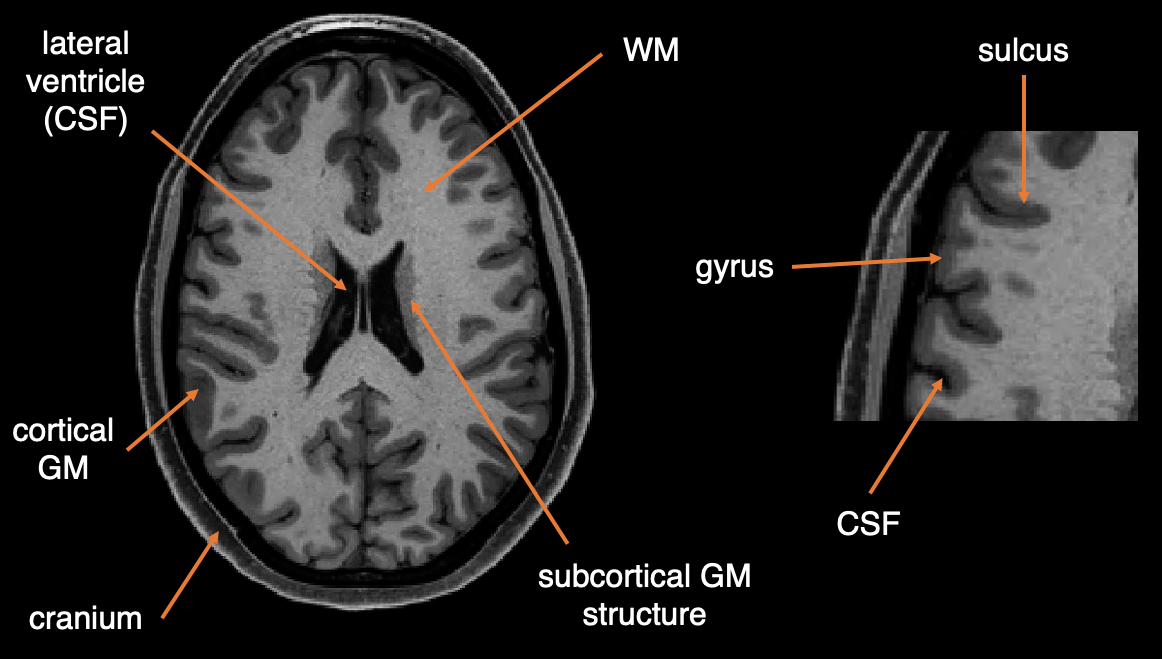
\includegraphics[width = \textwidth]{anatomy.png}
\caption{Left: High-level anatomy of the brain, showing the location of GM (cortical and subcortical), WM and CSF. Right: detail of the cortex, showing sulci and gyri.}
\label{anatomy}
\end{figure}

In a broad manner of speaking, the cortex performs many important tasks of cognition and accordingly it has been the focus of much research in neuroanatomy and brain function. To this end, researchers have identified numerous small and functionally distinct areas of cortex, for example the visual and auditory cortex, which process and respond to visual and aural stimuli respectively. Such a segmentation by function is commonly referred to as a \textit{parcellation} and an example is the Human Connectome Project's (HCP) multi-modal parcellation \cite{Glasser2016}, illustrated in figure \ref{fig_hcp_mmp}. In consequence of its many functions, the cortex is very physiologically active and has a high metabolic demand for oxygen and glucose, delivered via blood. Each of these metabolic demands can be used as a basis for physiological imaging, namely: 

\begin{itemize}

\item blood-oxygenation level dependent magnetic resonance imaging (BOLD MRI) is sensitive to the changes in blood oxygenation that accompany neuronal activation \cite{Jenkinson2017a}; 

\item fluorodeoxyglucose positron-emission tomography (FDG PET) is sensitive to changes in glucose metabolism \cite{Bohnen2013}; 

\item and arterial spin labelling MRI (ASL MRI) is sensitive to changes in blood delivery, a process called \textit{perfusion} \cite{Alsop2015}.  

\end{itemize}

\begin{figure}
\centering
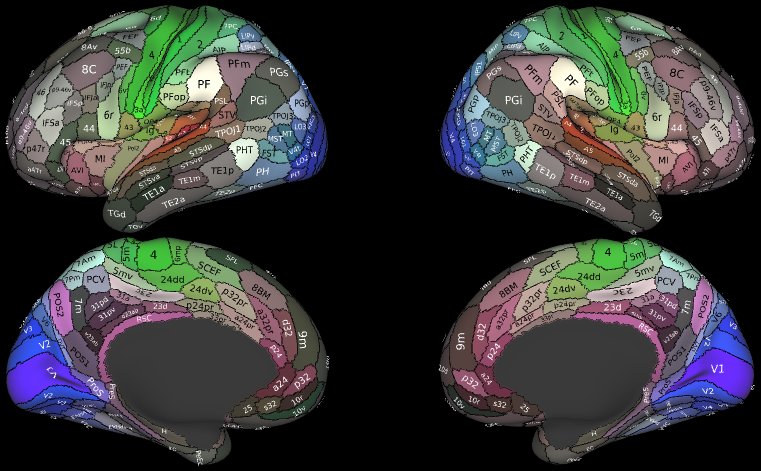
\includegraphics[width = 0.9\textwidth]{hcp_mmp.png}
\caption{The HCP-MMP parcellation of the left and right cortical hemispheres, coloured according to high-level function. For example, blue regions are associated with visual tasks. Reproduced with permission from \cite{hcp_mmp}.}
\label{fig_hcp_mmp}
\end{figure}

The function of WM in the subcortex may simplistically be described as providing connections between different parts of the cortex, and in consequence it is often discussed in context of the \textit{connectome}, a general term that describes the architecture of connections that form the basis of network-based models of cognition \cite{Sporns2005}. Though it is less physiologically active (being perfused at a lower rate than the cortex), it is by no means a passive tissue and is the focus of increasing amounts of research, particularly concerning neurodegenerative disease. For example, degradation of the myelin sheaths that surround axons plays a key role in multiple sclerosis \cite{Shafee2015}. As a result of its reduced levels of activity compared to the cortex, it can be challenging to perform physiological imaging in WM (the signal to noise ratio is inherently lower for some modalities). 

\section{Physiological imaging via arterial spin labelling}

Arterial spin labelling is a physiological imaging modality that uses magnetic resonance to produce signal. In common with other physiological imaging modalities (notably, PET), signal is acquired in a volumetric manner. The imaging region is divided into a regular grid of discrete subunits (voxels) within which signal is aggregated. The resultant data is stored as a three-dimensional matrix (with time acting as a fourth dimension where necessary) that matches the discretisation of the imaging region.

\subsection{The magnetic resonance signal}

Magnetic resonance imaging (MRI) is a non-invasive volumetric imaging technique that uses the magnetic properties of hydrogen nuclei\DIFaddbegin \footnote{\DIFadd{Any nuclei with non-zero spin may be used as a basis for MRI; due to the abundance of hydrogen within the body medical applications commonly focus on this element.}} \DIFaddend to generate signal \cite{bushberg2011}. In the presence of an external magnetic field, a population of hydrogen nuclei, referred to as \textit{spins}, will align their spin axis with that of the field and precess in steady-state with a well-defined frequency. The principle of MRI is to disturb this steady-state with radio-frequency (RF) excitation pulses that match the resonant frequency of spins and measure the dynamics of how steady-state is restored. The strength of the resonance signal is determined by the density of spins present in the imaging region and two physical decay constants. Different forms of MRI are distinguished by the sequence of RF pulses that they use to excite spins and subsequently acquire signal. 

%\subsection{Image acquisition} 

%Starting from a condition of steady-state, spins are aligned with the external magnetic field along the longitudinal axis (corresponding to the scanner bore and the inferior-superior axis of the patient). An RF excitation pulse instantaneously `tips' them into a transverse plane, from which they will re-align themselves over time with the longitudinal axis. Whilst the spins are returning to steady state, they emit an RF signal in the transverse plane that can be recorded by a set of readout coils and ultimately be converted into an image. The time between successive RF excitations is known as repetition time (TR). Signal acquisition is performed a short time after an RF excitation pulse; the period is known as the echo time (TE). In order to improve image quality, many repetitions of the excite/acquire process are performed. TE tends to be on the order of tens of milliseconds, whereas TR is usually a few seconds.   

%A spatial encoding strategy is used to localise the MR signal with respect to the position of the imaging region from which it originated. As a necessary step in this process, the imaging region is discretised into a regular grid of volume element, referred to as voxels. The resultant image will contain the summation of all signal contributions within the region of space corresponding to each voxel. For structural MRI, voxel sizes are usually around 1mm isotropic. 

%Signal acquisition is performed in the frequency-phase domain and a spatial encoding strategy is thus required to map positions within the imaging region to positions within the frequency-phase domain. Though there are many strategies for doing so, a common and simple approach is to use a series of 2D `slice' acquisitions which are then stacked into a single 3D volume. Under this approach, the slices are conventionally acquired along the increasing z-axis, from inferior to superior as referenced to the patient. Within an individual slice, frequency gradients and phase offsets are used to encode positions on the x-y plane. A Fourier transform is then applied to the frequency-phase data to reconstruct individual image slices. MR images are volumetric in nature and are comprised of many individual `voxels' (volume pixels). Voxels are a property of the spatial encoding strategy that was used to acquire the image and represent the discretisation of real space over which the MR signal was sampled. For typical anatomical MR scans, the voxel size is on the order of 1mm isotropic. 

\subsection{Control of contrast}

MRI allows image contrast to be controlled according to the magnetic properties of tissue. The resonance signal is subject to two forms of exponential decay, named T1 and T2 after the time constants that govern them. T1, or longitudinal, decay is the process by which a population of spins return to their equilibrium state following an excitation RF pulse. T1 is usually on the order of 1 - 2s for human tissue \cite{Alsop2015}. T2, or transverse, decay is the process by which a population of resonating nuclei de-phase relative to each other whilst out of alignment with the external field, thereby reducing the strength of their overall signal. T2 is on the order of 100ms for human tissue \cite{Buxton2009}. Strictly speaking, transverse decay is governed by a more complex constant called T2*, however commonly-used refocussing strategies remove the effect of this constant and it is therefore left out of this overview \cite{bushberg2011}. 

Two parameters of an MRI acquisition, referred to as the echo time (TE) and repetition time (TR), can be varied to maximise contrast as a function of tissue T2 or T1 respectively. For example, if TR is set to be many periods of T1, e.g. 7s, then all tissues are said to `fully relax' in the period between successive excitations and there will be little contrast arising from T1 differences. Conversely, for a short TR of 2s there will be some tissues that relax more than others, leading to greater image contrast. Control over contrast in this manner is referred to as \textit{weighting} the image; examples of T1-weighted and T2-weighted structural MRI scans are given in figure \ref{t1t2_image}. 

%\begin{table}
%\centering
%\def\arraystretch{1.5}
%\begin{tabular}{p{1cm} | p{6cm} | p{6cm}}
%& Short TE & Long TE \\
%\hline
%Short TR & T1-weighted: little de-phasing (T2) but tissues cannot fully relax longitudinally (T1)   & Mixed T1 and T2 image \\
%\hline
%Long TR & Proton density image: little de-phasing (T2) and full relaxation (T1) & T2-weighted: significant dephasing (T2) and full relaxation (T1)
%\end{tabular}
%\caption{TE and TR combinations to vary image contrast in MRI}
%\label {tableImageWeighting}
%\end{table}

\begin{figure}[h]
\centering
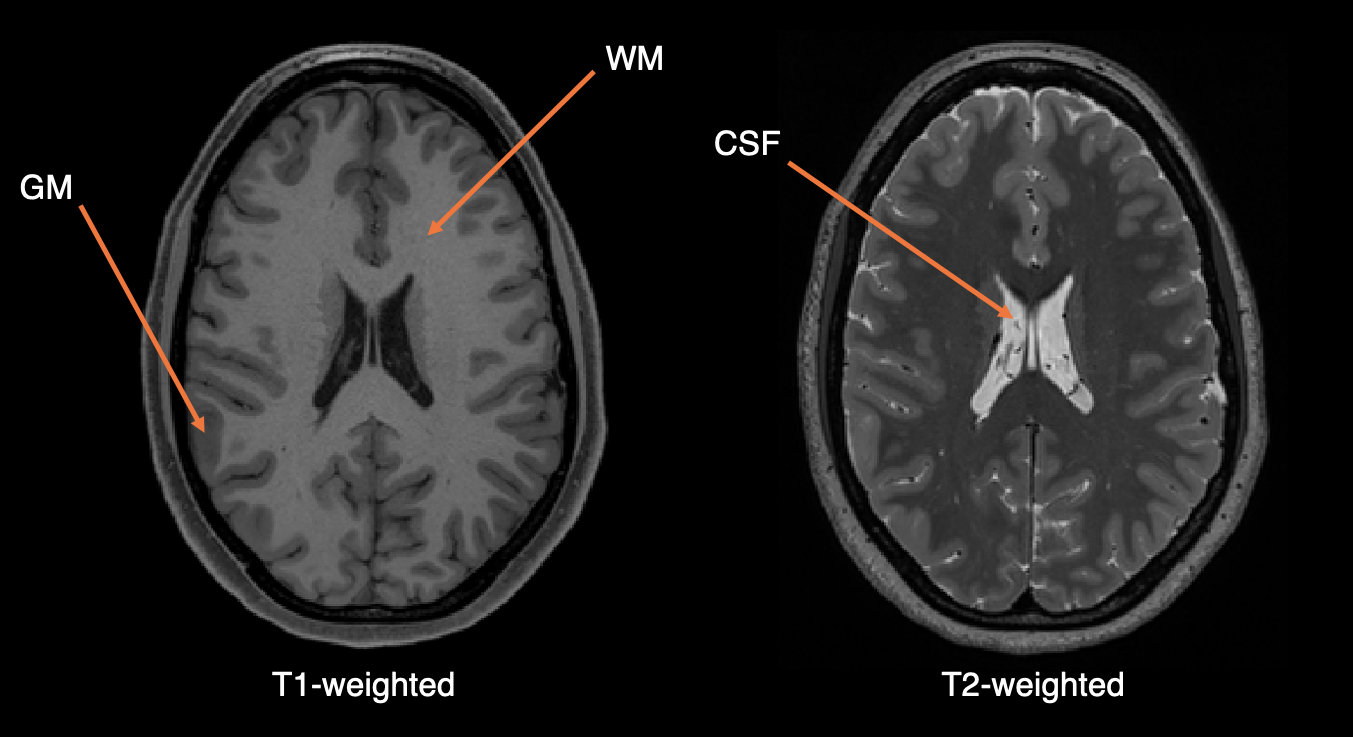
\includegraphics[width = \textwidth]{t1t2.png}
\caption{T1-weighted and T2-weighted structural MR images for subject 103818 of the HCP. Tissue intensities are broadly inverted between the two weightings (for example, CSF is dark on the T1w and light on the T2w), demonstrating how image contrast can be varied according to the T1 and T2 properties of tissue.}
\label{t1t2_image}
\end{figure}


\subsection{The arterial spin labelling signal}

Arterial spin labelling (ASL) is a non-invasive MRI technique that uses arterial blood-water as an endogenous contrast agent to measure the dynamics of perfusion \cite{Alsop2015}. Using magnetic fields, it is possible to magnetically `label' blood, follow its subsequent progression through the vasculature and exchange into tissue (the process of perfusion). Two parameters are of particular interest: cerebral blood flow (CBF) is the rate of blood delivery per unit weight of tissue, and arterial transit time (ATT) is the time taken for blood to traverse the vasculature.  

An ASL acquisition entails gathering many \textit{label} and \textit{control} image pairs \cite{asl_primer}. Using ASL applied to the brain as an example, a labelling region is defined across the neck perpendicular to the carotid arteries that supply blood to the brain. Prior to each label image acquisition, RF energy is applied within the region to invert the magnetic moment of spins that are present. The labelling itself may be instantaneous (referred to as pulsed ASL, pASL, in which case the region is a few centimetres thick) or maintained for a set length of time (referred to as continuous or pseudo-continuous ASL, pcASL, in which case the region is a plane of negligible thickness). The two labelling strategies are illustrated in figure \ref{label_regions}. The total quantity of blood that is inverted is referred to as the \textit{bolus} of label and is typically measured by duration, for example, a bolus of duration 1s. For pASL, the bolus duration is necessarily an approximate quantity as an entire spatial region is inverted instantaneously in time, though there are strategies that can be used to give a better-defined bolus duration (for example, QUIPSS II \cite{asl_primer}). 

\begin{figure}[h]
\centering
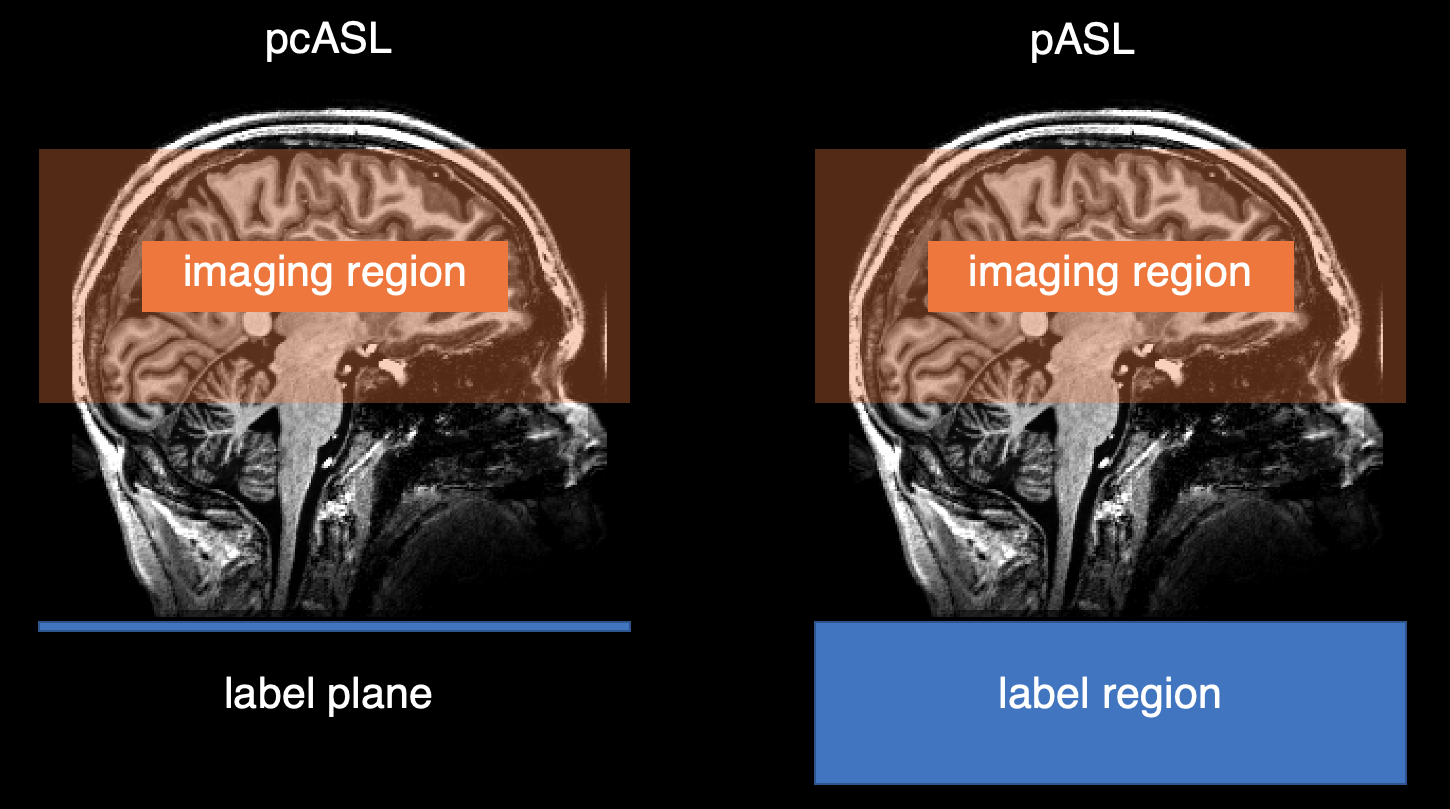
\includegraphics[width = \textwidth]{pcasl_pasl_regions.png}
\caption{Imaging and label regions for pcASL and pASL. For pcASL, the labelling is performed across a plane for a set time, for pASL it is performed instantaneously within a region.}
\label{label_regions}
\end{figure}

After labelling, a further period of time (known as the inversion time, TI, for pASL, or post label delay, PLD, for pcASL) elapses before image readout is performed. The TI/PLD allows the label bolus to traverse the arterial network and be delivered to the capillary bed of cerebral tissue (the length of time this requires is the arterial transit time, ATT). The entire process of label creation to readout leads yields a single label image. A control image is acquired in the same manner, except no RF inversion is applied and no label is created. The two images together comprise a label-control pair, the smallest unit of data required for the measurement of perfusion via ASL. 

Perfusion leads to the delivery of label, i.e. magnetically inverted spins, to the capillary bed, after which it exchanges into cerebral tissue. In the ideal case, when a label and control image are subtracted from each other, any cerebral tissue that was not perfused will have the same magnetisation on both images and produce zero difference signal. By contrast, tissue that has been perfused will have a lower magnetisation on the label image and hence produce a non-zero difference. The result of a label-control subtraction is referred to as a perfusion-weighted image and is the simplest possible indicator of perfusion available from ASL data, though it does not give quantitative estimates of CBF or ATT directly. 

The subtraction of a label-control pair yields a very weak signal. The difference image typically has around 1\% of the signal magnitude of the control image itself, and as such ASL suffers from intrinsically poor signal-to-noise-ratio (SNR) \cite{Li2018}. Based on the assumption that noise within an ASL acquisition follows a zero-mean Gaussian distribution (additive `white' noise) a number of strategies may be used to overcome this. Firstly, multiple label-control pairs can be acquired, across which the effects of noise should average out (taking multiple measurements of a noisy signal should yield the underlying true value, as is illustrated in figure \ref{single_multi_noisy}). Secondly, creating larger label boluses directly increases the magnitude of the difference signal. Finally, increasing the voxel size of the acquisition causes the difference signal to be sampled over a larger volume of space per voxel, which again causes noise to average out. It is for this latter reason that ASL data tends to have much larger voxel sizes than structural MRI (3-4mm vs. 1mm). Each of these strategies imposes a penalty: the first two directly increase the total duration of the acquisition, whereas the latter reduces the ability to resolve spatial details within the image. 


\subsection{The kinetic model for ASL} 
\label{asl_kinetic_section}

With appropriate processing, label-control difference images may be used to give absolute quantification of CBF and ATT \cite{asl_primer}. This is achieved by fitting a kinetic model of perfusion to the data in order to estimate the physiological parameters of interest. This model (hereafter referred to as the general model) is developed by considering the delivery of label to, and removal from, each voxel of the imaging region. The former process is represented by the arterial input function (AIF) and the latter by the residue function. As is the case for other tracer imaging techniques, the general model is formed by the convolution of the AIF with the residue function \cite{Buxton1998}. Conceptually, this is equivalent to splitting the label bolus into infinitely many discrete time intervals that are delivered independently, letting each of them decay after arrival \textit{on their own time scale}, and then summing their individual contributions at all moments in time. 

\subsubsection{Arterial input function}

In the ideal case, the label bolus is perfectly rectangular in time and space: it arrives uniformly, continues to do so for a length of time equal to the bolus duration $\tau$, and then ceases. During the time period between label creation and arrival in the imaging region (the ATT, denoted $t_A$), the label bolus will decay due to T1 effects, with the rate fixed by the T1 value of blood. The AIF is therefore a time-shifted and decayed copy of the original label profile. For pcASL, each part of the bolus takes the same time to travel from the label plane to the imaging region (fixed by the ATT), so each part of the bolus experiences the same decay and the profile is rectangular. For pASL, in which all of the bolus is created \textit{at the same time}, the leading edge reaches the imaging region before the trailing edge and therefore experiences less decay. The profile is therefore a windowed exponential decay curve, with the length of the window equal to the bolus duration. These are both illustrated in figure \ref{aif_profiles} and their mathematical forms are given in equation \ref{aif_functions}. The magnetisation of blood within the labelling region is denoted by $M_{0a}$. It is also possible to account for dispersion effects in the AIF (in reality, flow is non-uniform through the vasculature), though this effect is generally neglected \cite{asl_primer}. 

\begin{equation}
  a(t) =
  \begin{cases}
    0 & \text{for } t < t_{A} \\
    2M_{0a}e^{-(t-t_{A})/T_{1b}} & \text{(pASL) for } t_{A} \leq t < \tau + t_{A} \\
    2M_{0a}e^{-t_{A}/T_{1b}} & \text{(pcASL) } \\
    0 & \text{for } \tau + t_{A} \leq t \\
  \end{cases}
  \label{aif_functions}
\end{equation}


\begin{figure}[H]
\centering
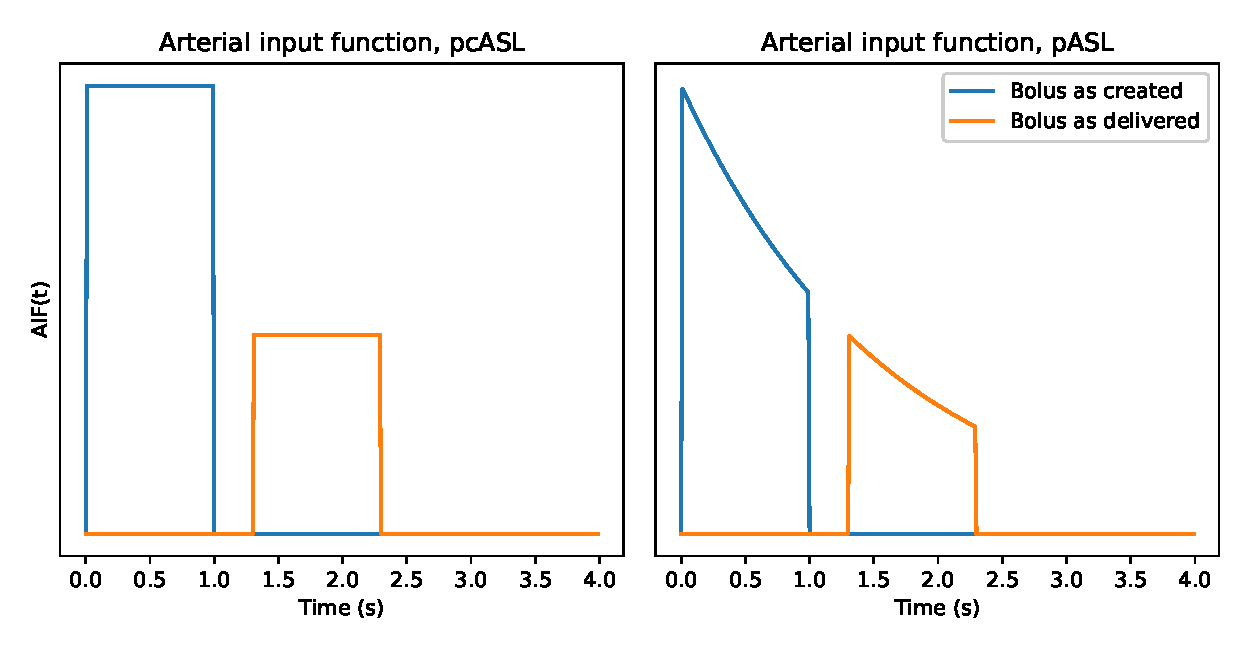
\includegraphics[width = 0.9\textwidth]{aif_profiles.eps}
\caption{AIF profiles for pcASL (left) and pASL (right) with 1s bolus duration and 1.3s ATT. The effect of T1 decay between label creation and delivery is shown; the rate of decay is fixed by the reference T1-blood value of 1.6s.}
\label{aif_profiles}
\end{figure}

\subsubsection{Residue function}

Upon arrival in the imaging region, the label bolus is removed by two processes. Firstly, it may leave by passing through the venous side of the capillary bed, a process that depends on the CBF $f$ of the voxel itself and also the partition coefficient $\lambda$, the relative concentration of water between the vascular space and tissue. Secondly, the label bolus will experience T1 decay, although the rate of this will now be fixed by the T1 value of the \textit{surrounding tissue}, not the T1 value of blood itself. This follows from the assumption that the exchange of label into tissue upon arrival in the voxel is fast; the voxel is said to be `well-mixed' \cite{Buxton1998}. The residue function is illustrated in figure \ref{residue_fig} and the mathematical form given in equation \ref{residue_eqn}. 

\begin{equation}
r(t) = e^{-tf/\lambda} \cdot e^{-t/T_{1}}
\label{residue_eqn}
\end{equation}

\begin{figure}[H]
\centering
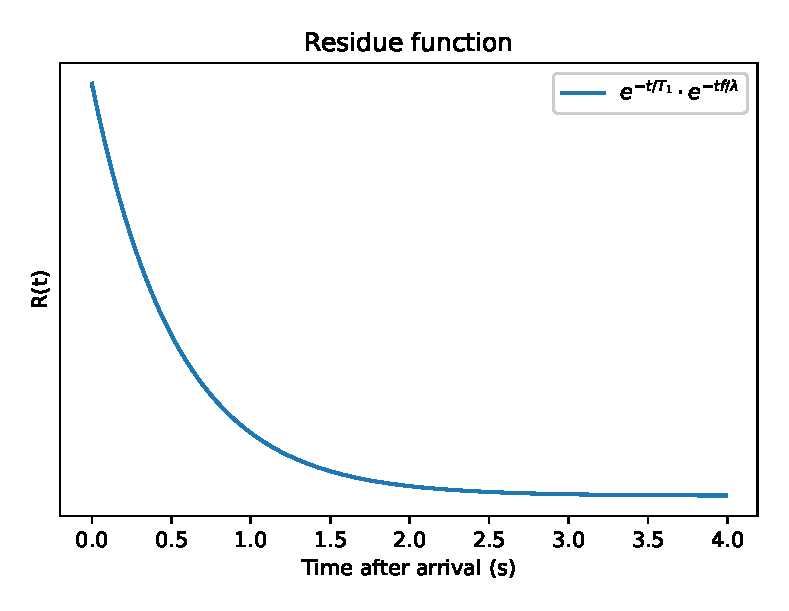
\includegraphics[width = 0.6\textwidth]{residue.eps}
\caption{Residue function for delivered label. The rate of decay is fixed by the T1 value of surrounding tissue; in this case the reference value of 1.3s for GM has been used, along with $f =$ \DIFdelbeginFL \DIFdelFL{1 }\DIFdelendFL \DIFaddbeginFL \DIFaddFL{60\cbf{}, which equates to 0.01s$^{-1}$, }\DIFaddendFL and $\lambda =$ 0.9 \DIFaddbeginFL \DIFaddFL{(dimensionless)}\DIFaddendFL .}
\label{residue_fig}
\end{figure}

Though the rate of exchange of label into tissue is generally fast enough in healthy subjects to justify the well-mixed assumption, some diseases may alter the permeability of the blood-brain barrier, in which case it would be necessary to update the residue function accordingly \cite{asl_primer}. 

\subsubsection{The general kinetic model}

The overall kinetic model is found by convolving the AIF and residue function to yield the equations given in \ref{pcasl_kinetic} (pcASL) and \ref{pasl_kinetic} (pASL). The difference in magnetisation arising from label-control subtraction is denoted $\Delta M$. These are illustrated for typical physiological and ASL parameters in figure \ref{kinetic_curves}. These equations are highly non-linear, which presents a challenge when attempting to fit the model to data in order to obtain parameter estimates. 

\begin{equation}
  \Delta M(t) =
  \begin{cases}
    0 & \text{for } t < t_{A} \\
    2 f M_{0a} T_{1app} e^{-t_{A}/T_{1b}} (1 - e^{-(t-t_A)/T_{1app}}) & \text{for } t_{A} \leq t < \tau + t_{A} \\
    2 f M_{0a} T_{1app} e^{-t_{A}/T_{1b}} e^{-(t - t_A - \tau)/T_{1app}} (1 - e^{-\tau/T_{1app}}) & \text{for } \tau + t_{A} \leq t \\
  \end{cases}
  \label{pcasl_kinetic}
\end{equation}

\begin{equation}
\frac{1}{T_{1app}} = \frac{1}{T_1} + \frac{f}{\lambda}
\end{equation}

\begin{equation}
  \Delta M(t) =
  \begin{cases}
    0 & \text{for } t < t_{A} \\
    2 \frac{f M_{0a}}{k} e^{-t/T_{1b}} e^{kt} (e^{-kt_{A}} - e^{-kt}) & \text{for } t_{A} \leq t < \tau + t_{A} \\
    2 \frac{f M_{0a}}{k} e^{-t/T_{1b}} e^{kt} (e^{-kt_{A}} - e^{-k(t_A + \tau)}) & \text{for } \tau + t_{A} \leq t \\
  \end{cases}
  \label{pasl_kinetic}
\end{equation}

\begin{equation}
k = \frac{1}{T_{1b}} - \frac{1}{T_{1app}}
\end{equation}


\begin{figure}[H]
\centering
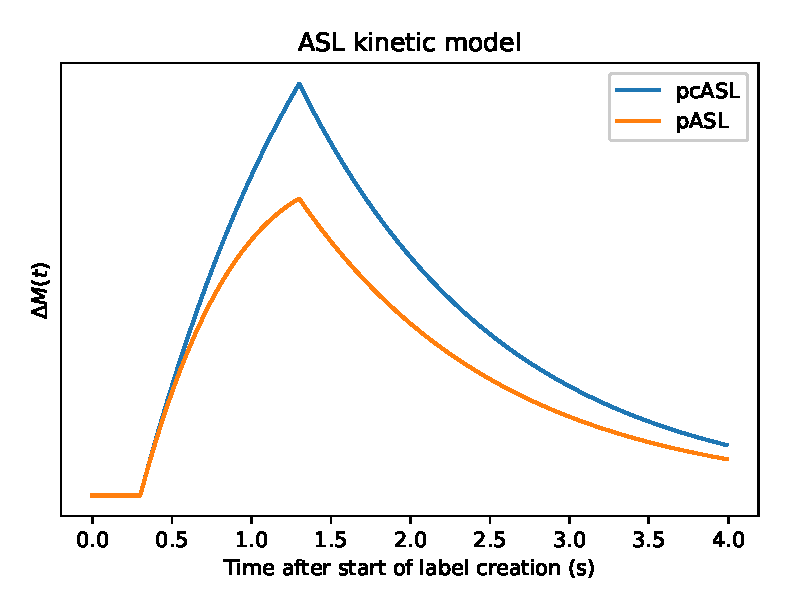
\includegraphics[width = 0.6\textwidth]{kinetic_curves.eps}
\caption{Kinetic models for pcASL and pASL with representative physiological and ASL parameters.}
\label{kinetic_curves}
\end{figure}

\subsubsection{Quantification with single- and multi-time imaging}

In light of the kinetic curves illustrated in figure \ref{kinetic_curves}, estimation of perfusion via ASL may be interpreted as a process of sampling different points on the idealised curves. The samples correspond to the subtraction of individual label-control pairs. Single-time imaging samples the kinetic curves at a single moment in time whereas multi-time imaging samples across multiple points in time (\textit{i.e.}, multiple positions on the $t$-axis). Although the former method is simpler, it naturally limits the number of parameters that can be estimated, whereas multi-time imaging allows estimation of both CBF and ATT. The difference between these two strategies is illustrated, along with the presence of acquisition noise, in figure \ref{single_multi_noisy}. 

\begin{figure}
\centering
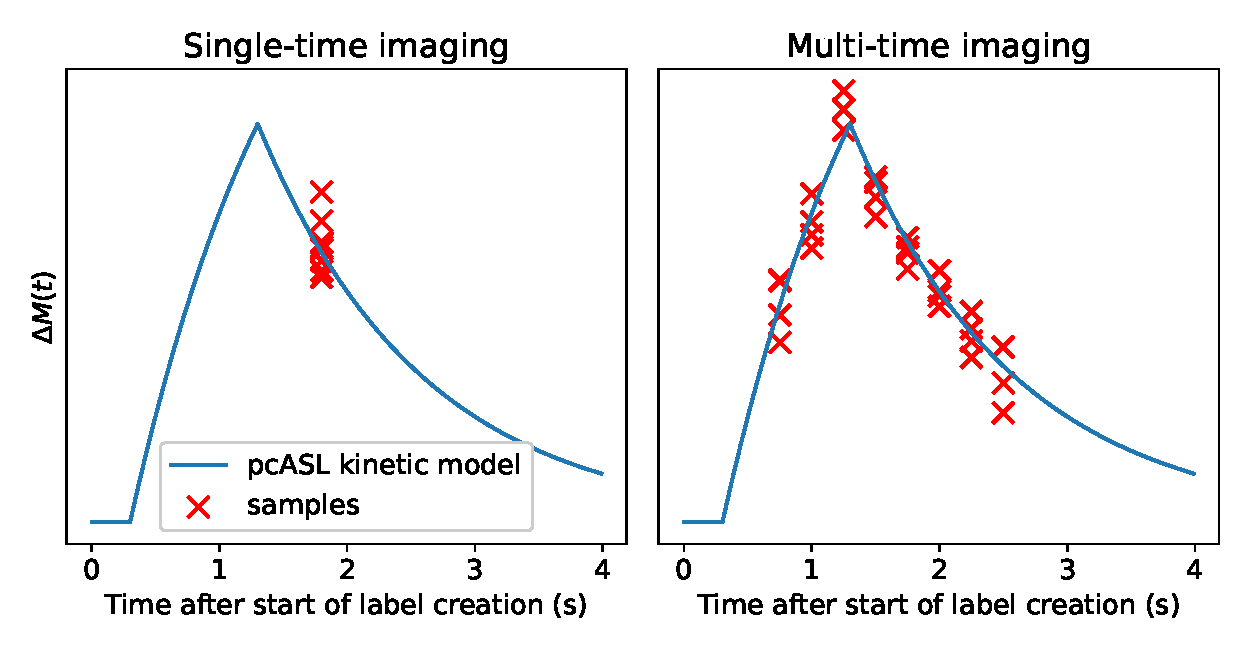
\includegraphics[width = 0.8\textwidth]{single_multi_noisy.eps}
\caption{Single- (left) and multi-time (right) imaging strategies. Multi-time better captures the shape of the kinetic curve and therefore allows for estimation of both CBF and ATT. For each case, the effect of white noise on the individual samples is shown. With sufficient samples, averaging at each sample time should yield the underlying signal value.}
\label{single_multi_noisy}
\end{figure}

\section{Parameter estimation via Bayesian inference}
\label{lit_vb}

In order to obtain parameter estimates (\textit{i.e.}, CBF, ATT, \textit{etc}) from physiological imaging data, it is necessary to \textit{fit} a model to the data. In the case of ASL, for which the kinetic model is non-linear, a widely used strategy is non-linear least squares fitting \cite{Chappell2009}. The drawbacks of such an approach are that it may not be robust in the presence of high noise, and that it does not allow for the incorporation of existing, or \textit{prior}, knowledge about what parameter values are plausible. 

An alternative approach to parameter estimation is based upon probability theory. The objective is to obtain a probability distribution on each parameter of interest. Such an approach acknowledges that, given acquired data, there are multiple values that each parameter could plausibly take, particularly in the presence of high noise. For example, in the case of the kinetic model for ASL, a high CBF and long ATT could be mistaken for low CBF and short ATT if one only had observations from a single moment in time; both are plausible parameter configurations given limited data. The advantage of using probability distributions on each parameter of interest is that it allows a `best' estimate, or most likely value, to be returned, as well as a measure of uncertainty on that estimate. 

There are two strategies for obtaining parameter estimates for a given model and acquired data. One approach deals with likelihood and answers the question \textit{what parameter values are most likely to produce the data that has been obtained?} The other approach deals with the posterior and answers the question \textit{given the data that has been obtained, what parameter values are most likely?} Though the difference is semantically subtle, there is an important mathematical distinction between the two that is readily \DIFdelbegin \DIFdel{be }\DIFdelend demonstrated via Bayes' theorem. Using the notation $y$ to denote the data that has been acquired (samples of the kinetic curve), $\theta$ to denote the parameters of interest (CBF, ATT, and potentially others), and $M$ to denote the generative model (the mathematical construct that maps $\theta$ to $y$, i.e., the kinetic model), an expression for the \textit{posterior} probability of $\theta$ is obtained as follows. 

\begin{equation} 
P(\theta | y, M) = \frac{ P(y | \theta, M) P(\theta | M) }{ P(y | M) }
\end{equation}

The term $P(y|\theta, M)$ is the \textit{likelihood} and is the focus of maximum-likelihood techniques, which make the assumption that the value of $\theta$ that maximises it will be approximately equal to the the value of $\theta$ at which the posterior is also maximal. However, two other terms modify the likelihood to give the posterior: the \textit{prior} $P(\theta | M)$ and \textit{evidence} $P(y | M)$. Because the evidence term simply acts as a linear scaling of the posterior (it is independent of the parameters $\theta$ that are sought), it is often neglected for simplicity. Similarly, because all terms have a dependence on $M$, it is often omitted from the notation for clarity. The posterior then becomes: 

\begin{equation} 
P(\theta | y) \propto P(y | \theta) P(\theta)
\label{eqn_bayes_posterior}
\end{equation}

This equation represents the basis of Bayesian inference methods. Note that when the prior is non-informative (represented by a uniform distribution), the posterior and likelihood terms will be linear mappings of each other (scaled by the evidence term); therefore likelihood and posterior based approaches are equivalent in this circumstance\footnote{For example, in the absence of any prior information, certain forms of Bayesian inference can be shown to be equivalent to non-linear least squares fitting \cite{Chappell2009}.}. 

There are three key advantages to using Bayesian inference over the more widely used maximum-likelihood methods. One is that it allows the incorporation of prior knowledge into $P(\theta)$ to guide the inference. The second is that it allows for an explicit treatment of acquisition noise (specifically, by incorporating it probabilistically into the generative model $M$). Finally, the inference process returns full parameter distributions as opposed to point estimates, which in turn enables the quantification of uncertainty on each parameter. For a technique that suffers from intrinsically poor SNR such as ASL, these features contribute to more robust parameter estimation. 

\subsection{Variational Bayesian inference}
\label{vb_section}

Although the equation underpinning Bayesian inference looks simple, in practice the technique can be difficult to implement analytically. This is because for all but the simplest models involving a low number of parameters and simple distributions, evaluating the posterior will entail performing an intractable computation. For example, if one wishes to ensure that the posterior is correctly scaled (all probability distributions should integrate to unity), then it is necessary to evaluate the evidence term $P(y | M)$ in the denominator of equation \ref{eqn_posterior_marginal}. This will entail the calculation of a marginal probability, as follows. 

\begin{equation} 
P(\theta | y, M) = \frac{ P(y | \theta, M) P(\theta | M) }{ P(y | M) }= \frac{ P(y | \theta, M) P(\theta | M) }{ \int_{\theta} P(y,\theta | M)P(\theta | M) \,d\theta }
\label{eqn_posterior_marginal}
\end{equation}

As the number of model parameters (dimension of $\theta$) increases, performing such integrations over a high dimensional space becomes infeasible. A number of approximative alternative strategies have therefore been developed, one of which is variational Bayesian (VB) inference. 

VB methods seek to approximate the true posterior using an arbitrary distribution $q(\theta)$, which itself is parameterised by a set of hyper-parameters (for example, $q(\theta)$ may be a normal distribution with corresponding mean and standard deviation, these latter quantities being the hyper-parameters). For \textit{each} parameter in $\theta$, there will be a corresponding distribution in $q(\theta)$ with a set of hyper-parameters. 

The quality of the approximation between $q(\theta)$ and the true posterior $P(\theta | y)$ may be quantified using the Kullback-Liebler (KL) divergence \cite{Wani2020}, defined in equation \ref{eqn_kl_div}. However, as calculating this quantity requires integration of the posterior $P(\theta|y)$ that is being sought in the first place, it cannot be directly evaluated. Nevertheless, with a quantitative measure of approximation quality thus defined, the inference process can be re-cast as an optimisation problem: what is the best approximation of the posterior, or, mathematically, \textit{what $q(\theta)$ minimises the KL divergence with the true posterior?}

\begin{equation} 
KL = \int q(\theta) \log{ \left[ \frac{ q(\theta)  }{ P(\theta|y) } \right] } \, d\theta
\label{eqn_kl_div}
\end{equation}

Minimisation of the KL divergence is equivalent to maximisation of a related quantity called the free energy \cite{Chappell2009}, defined in equation \ref{eqn_free_energy}. Crucially, all of the terms in this expression can readily be obtained: it is a function of the approximating posterior $q(\theta)$, the likelihood $P(y|\theta)$ and the prior $P(\theta)$. 

\begin{equation} 
F = \int q(\theta) \log{ \left[ \frac{ P(y|\theta) P(\theta) }{ q(\theta) } \right] } \, d\theta
\label{eqn_free_energy}
\end{equation}

This equation represents the objective of variational Bayesian inference: find the optimal $q(\theta)$ such that the free energy defined in equation \ref{eqn_free_energy} is maximised. Whilst it is not necessary to go into the mathematical details of how the optimisation is performed, a description of the process reveals the key assumptions that make this possible, and the restrictions they impose. 

\subsubsection{Mean field approximation}

In order to further simply the mathematics of VB inference, the mean field approximation is taken for $q(\theta)$. This entails splitting the parameters in $\theta$ into a number of independent subgroups $\theta_i$, which therefore means that $q(\theta)$ can be expressed as a product over the distributions of the individual subgroups. The practical impact of this is it reduces the number of terms that need to be calculated within the overall covariance of $q(\theta)$. A complete factorisation of all the individual parameters is not required \cite{Attias2000}. 

\begin{equation}
q(\theta) = \prod_i q_{\theta_i}(\theta_i)
\end{equation}

\subsubsection{Calculus of variations}

Maximisation of $q_{\theta_i}(\theta_i)$ over $F$ is obtained by applying the calculus of variations to yield a set of iterative update equations for the hyper-parameters of $q_{\theta_i}(\theta_i)$ \cite{Chappell2009}. The analytic form of these update equations follows from the choice of priors and likelihood that has been made. This is a crucial property of the VB framework and implies that if either the likelihood or priors are modified, then it is necessary to re-derive the update equations. 

The update equations for VB are generally not independent: the update for one $q_{\theta_i}(\theta_i)$ may depend on other $\theta_i$. As such VB follows the updating framework used by expectation-maximisation algorithms, in which the updates for all $\theta_i$ are performed using their values from the previous iteration, and so on until convergence.

\subsubsection{Conjugate exponential restriction}

In order to further simplify the derivation of the update equations on $q_{\theta_i}(\theta_i)$, a constraint on the form of the priors may be made such that they are conjugate with the likelihood \cite{Chappell2009}. \DIFdelbegin \DIFdel{This holds if and only if }\DIFdelend \DIFaddbegin \DIFadd{In this context, conjugacy means that }\DIFaddend the prior is of the same parametric form as the posterior (for example, both being normal distributions). For reasons of tractability, distributions are often chosen from the exponential family and hence this aspect of VB is often referred to as the `conjugate-exponential' restriction. 

\subsubsection{Non-linear models; convergence}

VB as presented thus far applies to linear models (i.e., the data is a linear mapping of the parameters with some noise contribution). As demonstrated in section \ref{asl_kinetic_section}, obtaining parameter estimates from physiological imaging data can require fitting a non-linear model; the general kinetic ASL model is just one such example. It is possible to perform inference on non-linear models by approximating them with a Taylor expansion. The approximation may be weakly non-linear (Woolrich and Behrens used a second-order expansion \cite{Woolrich2006}) or may be fully linear (both Friston \textit{et al.} and Chappell \textit{et al.} used first-order expansions \cite{Chappell2009, Friston2007}). 

In general, the iterative updates derived under VB are guaranteed to converge as they are fundamentally a generalisation of expectation maximisation \cite{Attias2000}. The drawback of using approximations to fit non-linear models is that this guarantee is broken: as the inference is on an approximation of the model, not the model itself, convergence cannot be ensured in any region where the model deviates from the approximation. This is not an insurmountable problem and multiple authors have incorporated a `trial' process into their implementations of VB in order to spot convergence issues \cite{Chappell2009, Friston2007}. 

Chappell \textit{et al.}'s implementation of VB will be used multiple times throughout this work. Specifically, this consists of two tools included within FSL: FABBER is the core VB model-fitting algorithm, whereas BASIL is a wrapper around FABBER that facilitates ease-of-use for ASL applications \cite{Chappell2009, Chappell2011}. 

\subsection{The role of priors}
\label{vb_spatial_prior}

Priors play a central role in Bayesian inference. They can be used to convey the existence of prior knowledge about what values a parameter could take (for example, based on anatomy or physiology), or equally they can be used to convey the absence of knowledge (so called non-informative priors will not steer the inference process in any particular direction). Priors can also be defined in a spatial sense, \textit{i.e.}, with reference to the spatial distribution of parameter values. This is especially important in the context of neuroimaging as it allows the application of a near ubiquitous data-processing operation - spatial smoothing - in a principled manner. Smoothing is commonly applied to physiological imaging data in order to mitigate low SNR based on a two-fold assumption: firstly, that noise within the data is not spatially correlated, and therefore will be reduced by smoothing, and secondly, that the length scale of parameter variance will be relatively low compared to that of the smoothing kernel \cite{Jenkinson2017a}. The first assumption may readily be justified by knowledge of the acquisition process, but the second presents a challenge: the amount of smoothing to apply is ultimately at the discretion of the investigator and it will unavoidably obscure at least some spatial detail. 

Within a Bayesian framework, the key aspect regarding smoothing is the \textit{belief} on which the operation is justified: significant parameter variation is not expected between neighbouring voxels. This may be encoded using a Laplacian spatial prior. Conceptually, the Laplacian measures the curvature of a function and therefore returns high values for functions that are varying quickly in space. By interpreting the parameter values within voxels as samples from an underlying parameter field (for example, the `CBF' field), the Laplacian can be used to measure the local curvature for all voxel neighbourhoods. A neighbourhood containing many different parameter values is not smooth and such a configuration is probabilistically unlikely, or, in the terminology of the VB optimisation, will have a high latent cost. It is this cost that drives the optimisation towards more likely (spatially smooth) configurations. The benefit of incorporating this prior into the VB framework (a modification referred to as spatial-VB within FABBER \cite{Chappell2011}) is that that the weight that is given to the prior (the \textit{spatial precision}) is itself a target of the optimisation, which in turn negates the need for the user to specify this ahead of time \cite{Penny2005}. In practical terms, the degree of smoothing will be \textit{data-driven} and determined by how informative the data is. As will be discussed in section \ref{fabber_pvec}, spatial priors also enable partial volume effect correction to be performed. 


\section{Partial volume effects}

\subsection{Origin}

Physiological imaging techniques tend to use larger voxel sizes (around 3-4mm side length) than those used for structural imaging in order to improve SNR. As voxel sizes approach the length scale of structures of interest within the imaging region, individual voxels \DIFdelbegin \DIFdel{more are }\DIFdelend \DIFaddbegin \DIFadd{are more }\DIFaddend likely to intersect multiple structures and therefore contain a mixture of different tissues. The proportions of different tissues inside a given voxel are called partial volumes (PVs). In the context of brain imaging, the cortex is a structure of particular interest but presents a challenge because its mean thickness of 2.5mm in adults is approximately equal to voxel size \cite{Fischl1999a}.  

PVs give rise to a source of confound for the analysis of physiological imaging data because they pose a mixed-source problem: within each voxel, there are multiple sources (tissue types) but one measured signal (a sum weighted by the partial volumes of tissue in that voxel). This mixing is called the partial volume effect (PVE). It is desirable to know the physiological activity in each tissue separately; to do so it is necessary to un-mix the signal via partial volume effect correction (PVEc). \DIFaddbegin \DIFadd{Both ASL and PET suffer from PVE as they record a signal of interest in both GM and WM. The situation with BOLD is somewhat different: though both GM and WM within a voxel may contribute signal, the analysis of such data tends to focus on the contribution made by GM only. Hence, for this modality, PVEc may be better understood as a noise-reduction process (removing the nuisance signal arising from WM) rather than separating out two distinct signals of interest. 
}\DIFaddend 

PVE arise due to the highly specific interaction of a subject's anatomy, their location within an imaging matrix, and the imaging modality. Accordingly, for a given modality and imaging matrix, changes in subject anatomy over time will modify the distribution of PVE within the acquired data. This is especially the case for longitudinal studies of neurodegenerative disease such as Alzheimer's disease, which is characterised by the atrophy (thinning) of cortical GM regions \cite{Thompson2003}. For a given voxel intersecting such a region, the measured signal will decrease over time due to the reduced volume of cortex within that voxel. This introduces a source of negative bias into measurements, even though the tissue that \textit{does} remain in the voxel may be contributing proportionally the same amount of signal as before. Such a bias could obscure patterns that may be of interest when investigating biomarkers of disease \cite{Thomas2011}. 

\subsection{Partial volume estimation}

Any form of PVEc requires a set of PV estimates within the same voxel voxel grid as the physiological data as a point of departure. In essence, this is an explicitly volumetric representation of the problematic anatomy for which PVE have arisen. As this entails classification of the tissues (and their proportions) that are present in each voxel, this is closely related to image segmentation. It should be noted that PV estimates are specific to each acquisition, because they arise due to the acquisition-specific intersection of subject anatomy with the imaging matrix. 

Given the similarity with volumetric segmentation, many PV estimation techniques have used the same theoretical basis as segmentation methods. This includes Gaussian mixture model methods which treat the histogram of structural image voxels as the superposition of three individual Gaussian distributions corresponding to the dominant tissue classes (GM, WM, and CSF). The process of segmentation is then framed as determining to which distribution a given voxel is most likely to belong, based on its intensity. Santago and Gage provide a reference implementation of this approach \cite{Santago1993}. Though this concept can clearly be extended to PV estimation, there is a subtle difference between the two: segmentation aims to assign a \textit{single} label to a voxel, and therefore attempts to match it to a \textit{single} distribution, whereas PV estimation starts with the premise that there can be \textit{multiple} tissues present in a voxel. Furthermore, a 70\% chance of a voxel belonging to given tissue class does not necessarily imply that the voxel is 70\% comprised of that tissue, though some first-order relationship between the two could reasonably be assumed. A more direct treatment is to introduce explicitly mixed tissue distributions (\textit{e.g.}, GM and WM) into the framework, however due to the minimal divergence between multiple such distributions Santago and Gage found that the overall performance of this variant was worse than in the three-tissue case \cite{Santago1993}.

Despite their clear theoretical simplicity, mixture models, and more broadly histogram-based methods in general, face a fundamental challenge due to how PVE manifest themselves in the data. As illustrated in figure \ref{ideal_imperfect_pve_hists} on a simulated T1 anatomical image at high resolution, PVE can be thought of as increasing the within-class variance of samples drawn from an otherwise homogenous (low variance) tissue distribution. Visualised on a histogram, any amount of PVE is expected to lead to a broadening of the peaks that correspond to the pure distributions of each tissue. The challenge is that numerous other real-world effects also lead to the same outcome: for example, the presence of field inhomogeneities, acquisition noise and natural variability within tissue also increase the within-class variance of each tissue distribution (though many methods do attempt to account for these separately). Therein lies the difficulty: the basis in which mixture-model based methods seek to identify a partial volume voxel (the extent to which the voxel does not belong to any of the pure tissue distributions), is the very same basis on which other imperfections manifest themselves, leading to unavoidable ambiguity. In figure \ref{ideal_imperfect_pve_hists}, the idealised histogram corresponding to perfectly homogenous tissue distributions at high resolution is modified in two equivalent ways: firstly, by introducing high within-class variance but maintaining the same spatial resolution; and secondly, by introducing low within-class variance but also downsampling to reduce spatial resolution. Only in the latter case are PVE actually increased, but the outcome is similar in either case. 

\begin{figure}
\centering
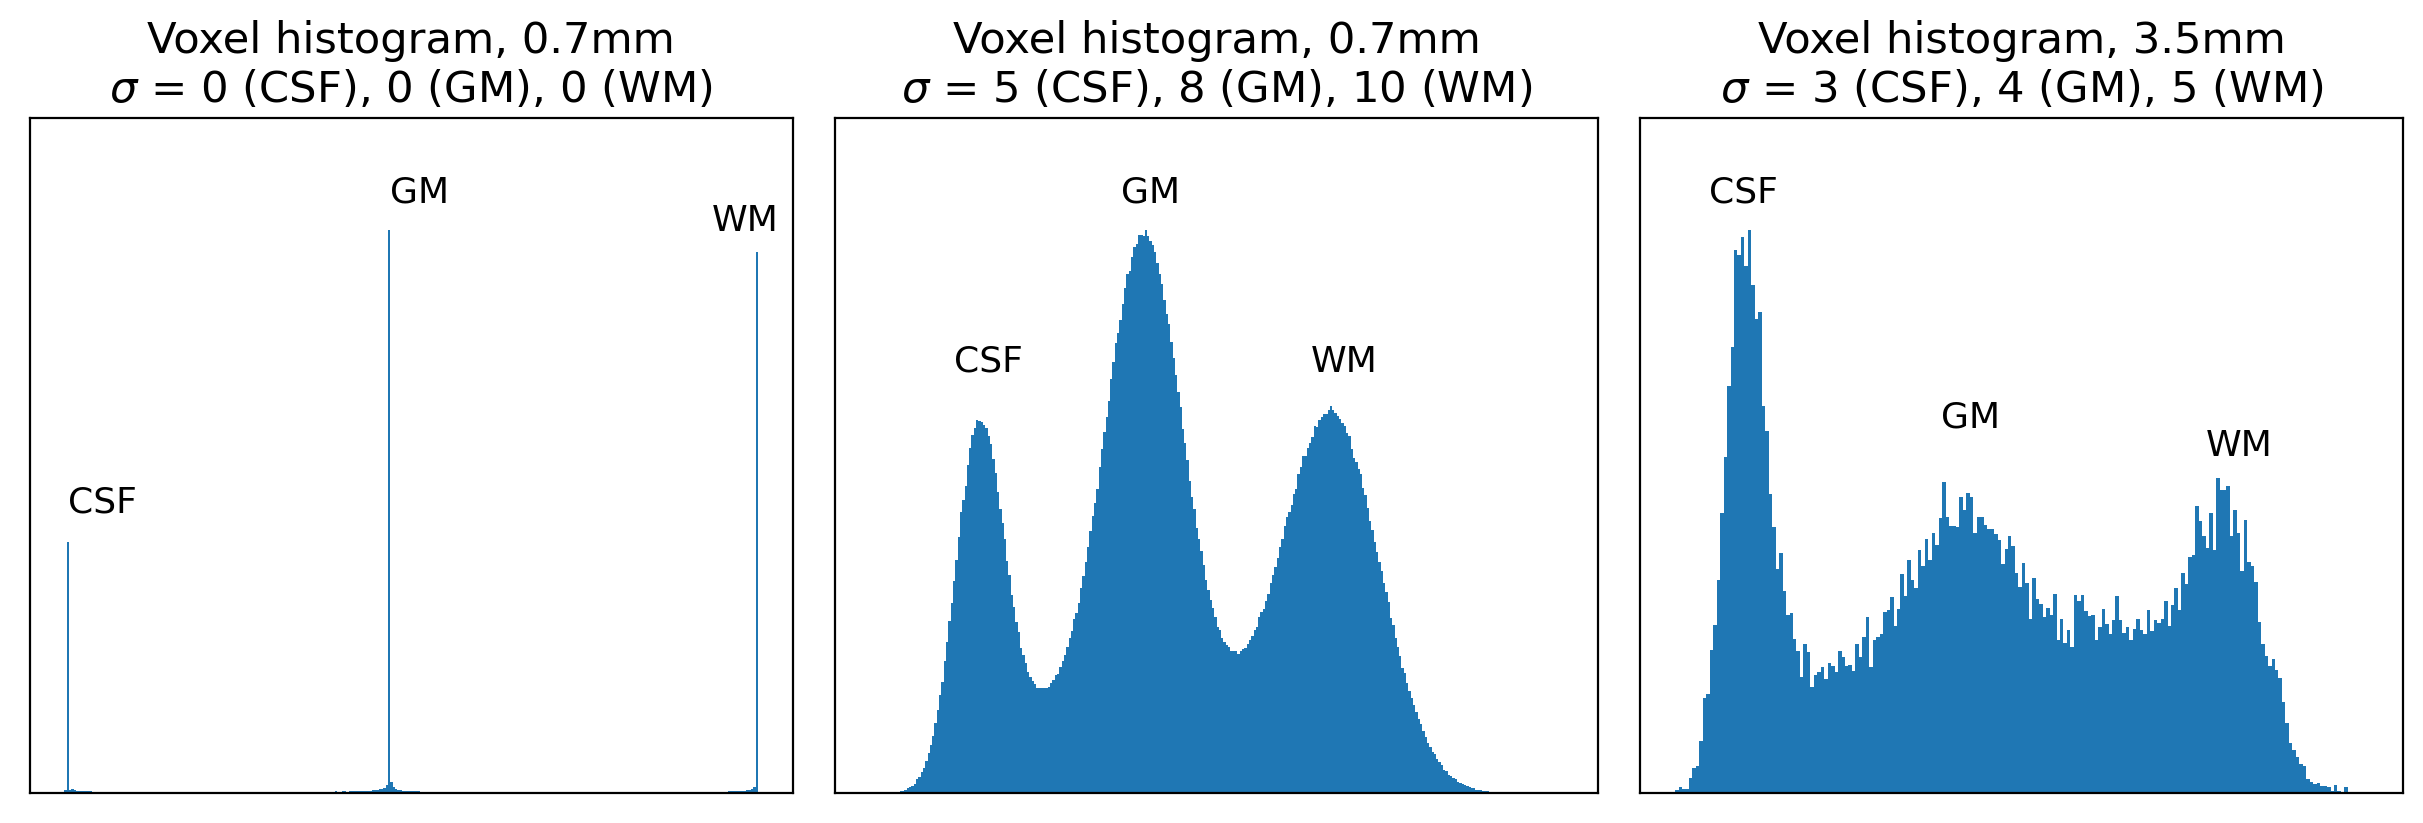
\includegraphics[width = \textwidth]{ideal_imperfect_pve_hists.png}
\caption{Left: voxel intensity histogram for a simulated T1 image at 0.7mm isotropic resolution with no within-class variance. Very few voxels contain PVs and therefore three sharp peaks are observed. Centre: histogram for a simulated T1 image at 0.7mm isotropic resolution, incorporating high within-class variance to represent real-world effects and imperfections. Numerous voxels lie in between the peaks corresponding to each tissue class. Right: voxel histogram for a simulated T1 image at 3.5mm isotropic resolution, with low within-class variance. Due to the much higher presence of PVE at low resolution, this histogram is similar in nature to the central plot; this demonstrates the difficulty of distinguishing PVE from other sources of variability.}
\label{ideal_imperfect_pve_hists}
\end{figure}

Segmentation and PV estimation techniques can also make use of spatial information in order to improve accuracy (so-called spatial mixture models). In keeping with the concepts presented in section \ref{vb_spatial_prior}, a spatial prior can be used to encode the belief that tissue classification should generally be homogenous across neighbourhoods of voxels, particularly if the length scale of voxels is small compared to the structures of interest (as is generally the case for structural MRI). FSL's FAST segmentation tool uses Markov random fields within an expectation maximisation framework to implement such an approach \cite{Zhang2001}. The same approach has also been implemented within a VB framework \cite{Woolrich2006}. The limitation of this strategy is that the belief it is founded upon - neighbourhoods of voxels should generally share similar classifications - is somewhat in contradiction to the very essence of PVE, namely that voxels may actually contain different tissues. A more fundamental point is the fact that the spatial prior is necessarily enforced in an isotropic manner at all locations within the brain. Deep within the large WM tracts of the subcortex, this is eminently appropriate, whereas at the deepest part of a sulcal pit, a sharp transition of tissue-type is expected and the assumption does not hold so well. 

The methods discussed thus far share the common property of being designed to work on structural resolution T1w images (though some also make use of the equivalent T2w images to exploit differing contrast). This is logical given that such images provide  high SNR, good tissue contrast and fine resolution for capturing spatial details. Accordingly, the PV estimates are returned in the same voxel grid as the anatomical image. For the purposes of PVEc, however, what is required are PV estimates in the same voxel grid as that of the data to be corrected, \textit{i.e.}, that of the physiological data. Resampling (a 3D interpolation operation) is therefore required to transform PV estimates from their native voxel grid to that of the physiological data. Due to the fact that the structural image may not be in alignment with the physiological data, a registration transformation may also be applied at the same time, so that the PV estimates are both transformed in space and resampled onto a new voxel grid; in either case, an interpolation is required. 

Due to the inherent resolution mis-match between structural MRI data and physiological imaging data, it is possible to derive PV estimates in the voxel grid of the physiological data using only a hard tissue segmentation (\textit{i.e.}, whole-voxel single-tissue labels). Because physiological imaging voxels tend to be much larger than structural voxels, each physiological voxel will enclose the same region of space as numerous structural voxels. A PV estimate for the larger voxel can therefore be obtained by simply counting the individual tissue labels of the corresponding structural voxels, without \DIFdelbegin \DIFdel{needing to explicitly perform }\DIFdelend \DIFaddbegin \DIFadd{explicitly performing }\DIFaddend PV estimation on the original structural data. Resampling tools such as FSL's \textit{applywarp} perform this summation over voxel neighbourhoods when dealing with mis-matched resolution data in order to better capture PVE \cite{Andersson2010}. The PVEc tools included with PETSurfer also derive their PV estimates in this manner \cite{Greve2016}, namely via FreeSurfer's binary segmentation at structural resolution. 

\DIFaddbegin \DIFadd{It should be noted that this latter approach is approximative and its appropriateness is determined in part by the degree of resolution mis-match (with a larger physiological voxel size, the mean field approximation implies that individual errors at the structural voxel resolution will average out). Furthermore, though single tissue labels are often assigned on the basis of a class-wise probability estimate, these cannot be assumed to map directly onto PV estimates. For example, a 70\% chance that a voxel belongs to the GM class does not mean that the voxel is 70\% GM, particularly if the mixture model framework that was used to derive the probability estimate included mixed tissue classes. 
}

\DIFaddend The method introduced by Ahlgren side-steps the need for resampling entirely by estimating PVs in the native space of an ASL acquisition \cite{Ahlgren2014}. This is achieved via the use of a T1-mapping approach applied to ASL data obtained via a QUASAR sequence. Because both the PV estimates and the ASL data to be corrected are derived from the same acquisition, there is no need to perform a registration or transformation, which therefore removes the possibility of this step introducing error. Unfortunately, this approach is restricted to use only with QUASAR data and the segmentation algorithm used is simplistic. 

\subsection{Correction methods}

Due to the fact that both ASL and PET suffer from PVE (in slightly different forms), numerous correction strategies for both modalities are reported in the literature. Examples of both will be given here. 

As PVE are an example of a mixed-source problem, they naturally lead to an under-determined system of equations within each voxel. Neglecting any signal contribution from CSF (which is assumed to be inactive), the physiological activity $S$ in a voxel may be expressed as a linear sum. 

\begin{equation}
S = P_{GM} F_{GM}+ P_{WM} F_{WM}
\end{equation} 

$P_t$ is the partial volume of tissue $t$ within the voxel and $F_{t}$ the physiological activity associated with that tissue in isolation. There are infinitely many solution pairs of $F_{GM}$ and $F_{WM}$ that satisfy this equation; PVEc methods differ in how they select a single pair.

\subsubsection{Linear regression}

Linear regression (LR) methods assume that perfusion within GM and WM are constant within a 2D or 3D kernel of side length $n$, containing $N$ voxels in total, centred at the voxel in question (the kernel may include only direct neighbours, or first diagonals, \textit{etc}). Under that assumption - a spatial prior of local similarity - the equation can be expressed in matrix form as

\begin{equation}
\vec{s} = \mat{P} \vec{f^*}
\end{equation} 

where $\vec{s}$ is a vector of length $N$ containing individual voxel signals, $\mat{P}$ is a matrix of size $N$ x 2 containing PV estimates for the kernel, and $\vec{f^*}$ is a vector of length 2 containing the GM and WM parameter values of interest. This equation may be solved for $\vec{f^*}$ with the pseudo-inverse of $\mat{P}$ which is equivalent to a least-squares linear regression solution. The major drawback of this approach is the smoothing effect imposed by the assumption of constant perfusion within the kernel, the extent of which is determined by the kernel size. Given the poor spatial resolution of physiological imaging data, and the length scale of structures of interest in the brain, this approach poses a risk of smoothing over important detail in structures such as the cortex. Asllani provides a reference implementation of this method for ASL data \cite{Asllani2008}. 

Petr \textit{et al.} investigated an extension of the LR method \cite{Petr2010}. They approached the problem as one of noise reduction via smoothing (the inevitable consequence of performing linear regression over kernels). Their key contribution was to constrain the smoothing operation to minimise signal variation within tissue classes whilst avoiding mixing signal \textit{between} classes and respecting regional variations in perfusion. The authors argued that this would make it more appropriate than standard LR for cases of pathology where local anomalies in perfusion need to be detected. 

A further extension of LR was developed by Liang \textit{et al.} \cite{Liang2013}. Again addressing the problem of smoothing imposed by the assumption of constant CBF over spatial kernels, the modified trimmed least squares (mTLS) approach essentially seeks to perform outlier rejection when constructing kernels within each voxel neighbourhood. The smoothing imposed by LR is most severe when the voxels within a neighbourhood have very different values. Accordingly, mTLS iteratively constructs kernels that include only the most similar voxels to the one currently undergoing correction. The authors reported reduced smoothing and better preservation of details, especially around the edges of structures. The method does require one user-set parameter, though the optimal value for this has been determined empirically on both simulations and \textit{in-vivo} data. 

\subsubsection{Spatial-VB}
\label{fabber_pvec}

Spatial-VB sits within FABBER's implementation of VB for ASL, presented in section \ref{vb_section}. Rather than fitting a kinetic model for a single tissue to the data (with a single CBF, ATT, T1 value \textit{etc}), a model with separate components for GM and WM is fitted in proportion to the PV estimates present in each voxel\footnote{This is a two step process, with an initial fit performed in single-tissue mode that is used as the basis for a second fit in both GM and WM. In each case, the FSL tool BASIL uses FABBER to perform the fit.} \cite{Chappell2011}. In this circumstance, the spatial prior introduced in section \ref{vb_spatial_prior} plays a dual role. Whereas previously it was used to enforce similarity between voxels as a means of performing noise rejection, in this situation it also \textit{conditions} the inference problem. This means that it allows for the inclusion of neighbourhood voxels in order to solve the inherently under-determined system of equations that arise due to PVE. In practical terms, this is equivalent to assuming constant parameter values across the neighbourhood of voxels, as is the case for LR, but crucially the strength of this assumption is relaxed compared to the LR case. This is because the weight given to the prior is a property of the optimisation itself, determined from the data, which generally results in reduced levels of smoothing compared to LR. A somewhat counter-intuitive feature of this approach is that it entails fitting components for GM and WM in all voxels, regardless of which tissues are actually present. For example, in the case of ASL, this means GM CBF and ATT will be estimated even in voxels that do not contain any GM. Though seemingly paradoxical from an anatomical point of view, the situation may be thought of in terms of fields: there exists a GM CBF field across the entire brain, from which samples are drawn at specific locations where the GM PV is non-zero, and in other voxels the spatial-VB approach will interpolate in value derived from informative neighbours. 

\subsubsection{PETSurfer}

PETSurfer is a subset of tools embedded within FreeSurfer (introduced in section \ref{surface_segmentation}) for kinetic modelling and PVEc of PET data \cite{Greve2016}. The nature of PVEc for PET is slightly different than for ASL due to spill-in / spill-out effects. These arise due to the relatively high point-spread function (PSF) of PET data compared to the voxel size used for imaging; the voxel in which signal appears is thus not necessarily the same as that where the signal was created. In fact, the partial volume effect that arises due to the presence of multiple tissues within a voxel is referred to in the PET literature by the alternative name of tissue fraction effect (TFE); Erlandsson discusses these differences in greater detail \cite{Erlandsson2012}. Three PET-specific PVEc methods are implemented within PETSurfer: Meltzer (MZ), Muller-Gartner (MG), and symmetric geometric transfer matrix (SGTM); all of which attempt to deal with PSF issues in different ways. The former two methods can be used for voxel-wise analysis whereas the latter is restricted to region-of-interest analysis only. 

The MZ method addresses only the PSF effect and does not attempt to separate out tissue contributions \cite{Meltzer1990}. For ASL, the PSF is \DIFaddbegin \DIFadd{typically }\DIFaddend of lower importance \DIFdelbegin \DIFdel{and the TFEis the key driver of PVE}\DIFdelend \DIFaddbegin \DIFadd{than the TFE, although some readout sequences such as single-shot 3D GRASE do exhibit relatively high PSF in one spatial dimension}\DIFaddend . As part of the correction, the user is required to set a manual PV threshold on voxels at the edge of the brain (usually in the region of 10 - 50\% tissue). 

The MG method addresses the PSF effect and attempts to remove the contributions of WM and CSF to leave a pure GM signal \cite{Muller-Gartner1992a}. This is achieved by deriving a single global value for WM and CSF contributions (using appropriately drawn ROIs), subtracting this value from mixed voxels, and finally scaling the remaining signal to account for lost tissue volume. The assumption of a single global value for WM and CSF is clearly of high importance; the same could not necessarily be made of other modalities. Once again the user is required to set a manual threshold on voxels to exclude from the correction. 

The SGTM method \cite{Labbe1998} is conceptually similar to the LR method for ASL: a linear matrix system that relates signal in a set of ROIs to voxel values is formed. 

\begin{equation}
\vec{y} = \mat{X}\vec{\beta}
\end{equation}

$\mat{X}$ is the key construct that maps individual voxels to their respective ROIs in a manner that accounts for both PSF and TFE; $\vec{y}$ and $\vec{\beta}$ are voxel-wise data and the desired ROI signal values respectively. Because $\mat{X}$ is dependent on the PSF it may be badly conditioned (leading to noise amplification) or non-invertible \cite{Greve2016}. 

Though in principle these methods could be made to operate with other modalities, they would require some degree of manual tuning for optimal performance. Although SGTM has performed favourably in comparison studies \cite{Greve2016}, the fact that it does not permit voxel-wise analysis would be a significant hinderance for a modality such as ASL, where volumetric analysis is increasingly widespread\footnote{Often, ASL studies simply report overall CBF values within regions of interest as opposed to voxelwise maps. Nevertheless, the underlying parameter estimation required to obtain such summary statistics is volumetric in nature, \textit{i.e.}, mathematical operations on voxels of data.}.

\subsubsection{Impacts of PVEc}

Numerous authors have investigated the consequences and benefits of performing PVEc. Evidence from both the PET and ASL literature suggests that there are important analysis benefits that can be realised with PVEc, but careful decisions must be made about the methods used (and the assumptions they encode), especially for methods that require user-set parameters. Nevertheless, in spite of these risks, a soft consensus is emerging that the difficulties of performing PVEc are not sufficient to disqualify the operation entirely. 

Erlandsson's review of PVEc methods for PET concluded that it is an ``important aspect'' of quantitative analysis, though also lamented the lack of existing ``turn-key'' solutions. This lack was attributed to the various methodological challenges and implications that are posed by PVEc: a high reliance on accurate segmentation and registration (particularly between MRI and PET data), potentially high sensitivity to noise, and the difficulty of justifying the assumptions that are required \cite{Erlandsson2012}.  

More recently, Greve \textit{et al.} investigated correction of a PET ageing dataset and found that, in the absence of PVEc, the data was ``highly contaminated'' by anatomical changes; a bias that was successfully removed with PVEc \cite{Greve2016}. SGTM was reported favourably as it required the fewest assumptions and was the most robust, though at the cost of permitting ROI-based analysis only. They also reported a diversity of results across different PVEc methods, which they conclude ``mirrors the confusion found in the literature about ageing and metabolism'' \cite{Greve2016}. 

Thomas \textit{et al.} found PVEc to improve the quantitative accuracy of amyloid PET regional analysis \cite{Thomas2011}. Some of the assumptions made by PET-specific strategies were found to introduce biases that lead to erroneous inferences, though this was not the case for the more recent methods. As applied to a multi-subject dataset, PVEc increased inter-subject variability, though the authors believed the increase to be genuine, leading them to conclude that PVEc should be mandatory in clinical studies in consequence of the improved accuracy it offers. Taken together, the findings of both Thomas \textit{et al.} and Greve \textit{et al.} highlight the fact that successful PVEc requires careful consideration of the context-specific biological and technical factors that give rise to PVE \cite{Thomas2011, Greve2016}. 

For ASL, Petr \textit{et al.} \cite{Petr2018} investigated the accuracy of PV estimates derived from T1w images for the application of different forms of PVEc (including quasi-methods, such as simple thresholding over ROIs). Whilst they did find geometric distortion and differences in effective resolution between ASL and structural data introduce some error into CBF quantification, this was not a sufficient basis to abandon PVEc altogether: ``PVEc remains the most accurate way to calculate GM CBF''. Furthermore, they found the differences arising due to the ASL-T1w mismatch to be of similar magnitude to the effect sizes in many CBF studies, thereby emphasising the importance of PVEc as a means of increasing statistical power. 

A separate investigation by Petr \textit{et al.} on their extension of the LR PVEc method reported increases in SNR for acquisitions with less than 20 label-control repeats, though SNR decreased above this number (because the extra signal imparted by more repeats outweighs the loss of signal caused by excessive smoothing) \cite{Petr2010}. 

An evaluation of the LR and spatial-VB PVEc methods for ASL showed that spatial-VB better preserves spatial details than LR at the cost of higher sensitivity to noise \cite{Zhao2017a}. Both methods were shown to reduce inter-session variability (this is especially important for longitudinal studies). PVEc of either form was also shown to be sensitive to errors in the PV estimates themselves. 

Despite the evidence that PVE present a significant challenge for quantitative analysis of ASL, PVEc remains rare within clinical studies that make use of this modality (a methodological review performed in 2017 found that 5\% of clinical studies explicitly reported performing this step\footnote{A sample group of 39 studies was assembled in the following manner. Firstly, a search on Scopus for \textit{( ( asl OR “arterial spin labelling” ) AND ( “functional” OR “fMRI” ) AND “clinical” AND ( “brain” OR “cerebral blood flow” OR “CBF” ) ) year $\geq$ 2010} yielded 236 papers that were sorted by number of citations and the top 28 that contained experimental work with a clinical endpoint. To these were added 11 papers from the monthly ASL Network newsletter, drawn from the section \textit{cerebral blood flow studies; studies on special disease} and also having a clinical endpoint.}). Indeed, the recommended implementation for ASL in clinical use merely highlights PVE as a source of confound without addressing how PVEc should be performed \cite{Alsop2015}. 


\section{The surface paradigm}

Volumetric imaging techniques necessarily divide the imaging region into discrete subunits called voxels. Signals are aggregated within these voxels with no regard to the underlying anatomy (or anatomies) that have produced them. Finally, the data arising from such an acquisition is represented using a three or four dimensional matrix structure that matches the discretisation of space. Surface representations of data stand in contrast to this. Instead of discretising the imaging region into regular volume units, surface methods assume that signal originates from discrete areas lying on some topological plane (which may nor may not be closed). A basic assumption that underpins the surface approach holds that locations on a surface will correlate better according to geodesic distance (along the surface) than geometric (straight-line). For example, on the cortical surface, areas on opposite sides of a sulcus are close in a geometric sense but distant in a geodesic sense. Electroencephalography (EEG) provides a useful discussion point to illustrate the key concepts. 

EEG is concerned with electrical activity within the cortex. Electrodes are distributed across the scalp in a known configuration. Conceptually, the signal generation and acquisition system may be thought of as two concentric spheres with differing radii: the cortex lies inside the sphere defined by the electrodes, and the small distance between them is taken up by the cranium and CSF (which have some transfer function that maps cortical activation to observed signal at the electrodes). 

Given how the signal is generated and acquired, it would be illogical to try and represent the signals recorded by the electrodes in a volumetric manner, whereas a surface representation lends itself readily. This is not without challenges (for example, source reconstruction, the localisation of individual activations on the basis of their appearance at multiple electrodes simultaneously, is complex), but the representation of the data naturally fits the anatomy of the structure of interest. 

Although volumetric imaging techniques such as PET and MRI cannot readily be made to operate in a surface-based manner, it is possible to process, transform and analyse the data they produce in such a way. In order to do so, a number of building blocks are required: a means of generating the surfaces of interest (surface segmentation), a means of moving data from a volumetric to a surface representation (surface projection), and finally a means of analysing data on the surface (surface-based analysis). 

\subsection{Surface segmentation}
\label{surface_segmentation}

Segmentation in a volumetric sense involves assigning class labels to individual voxels, themselves the discretisation basis of the imaging region, so the process is inextricably linked to the voxel grid of the image itself. Surface-based segmentation is independent of the voxel grid of the data on which it is performed. The segmentation aims to identify the boundaries between different regions of tissue within the image, which are modelled as contiguous triangular meshes, the vertices of which are calculated with sub-voxel (i.e., continuous) precision. This is in contrast to volumetric segmentation in which boundaries are necessarily identified with whole-voxel (discrete) precision. 

Surface segmentation also allows for the incorporation of spatial and geometric constraints informed by anatomy. For example, FreeSurfer - a tool that enjoys especially widespread support within the literature - segments the cortex according to the principle that it lies in between two contiguous (topologically spherical) surfaces, one defining the WM/GM boundary and the other the GM/CSF boundary \cite{Fischl2012}. Example FreeSurfer surfaces are shown in figure \ref{fs_demo}. FSL FIRST uses shape-based models as priors to segment subcortical structures \cite{Patenaude2011}. Tissue continuity is enforced anisotropically in either case: the premise of surface segmentation is that tissue is homogeneous \textit{along} a surface but heterogeneous \textit{across} it. This contrasts with the spatial prior used by FSL FAST, for example, which is necessarily enforced isotropically, \textit{i.e.}, with no regard for the underlying anatomy. 

\begin{figure}
\centering
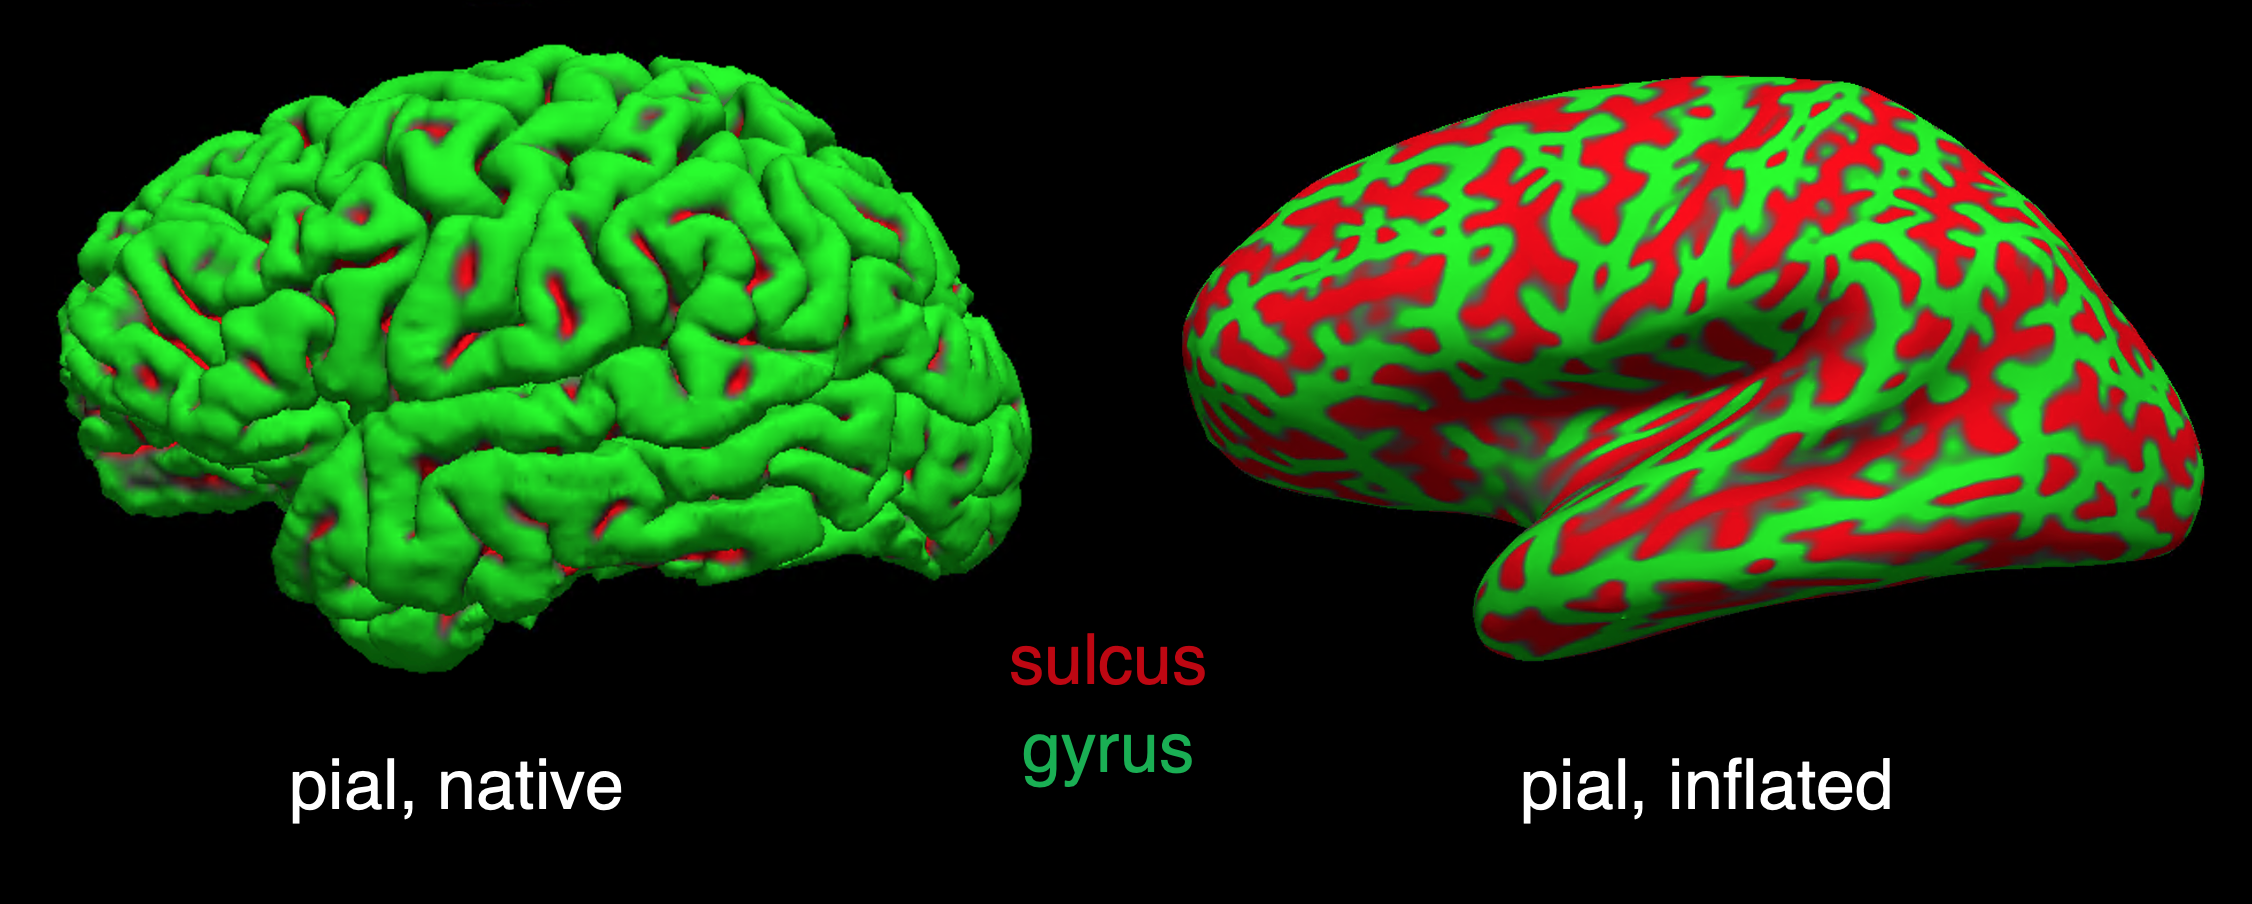
\includegraphics[width=\textwidth]{fs_demo.png}
\caption{Example FreeSurfer segmentations of the pial (outer) surface of the cortex. Both the native and inflated surface are shown; as there is vertex correspondence between the two, the inflated surface can be used to visualise data that would otherwise be obscured at the bottom of sulcal pits (highlighted in red).}
\label{fs_demo}
\end{figure}

Whilst the objective of surface segmentation is conceptually clear, there is a degree of subjectivity to it from an anatomical point of view: the notion of a hard border between WM and GM in the cortex is artificial and reality is better described by a gradient transition, albeit over a short length scale \cite{Dale1999}. Though it is difficult to determine with certainty whether surface or volumetric segmentation methods are more accurate for the cortex – defining an unambiguous ground truth for brain segmentation is challenging \cite{Shattuck2009} – the aforementioned characteristics of the surface-based approach suggest it is theoretically better suited to segmenting the cortex and it is well-established within the literature for this purpose. 

 
\subsection{Surface projection}
\label{lit_projection_methods}

Data that has been acquired in a volumetric manner must be transformed `onto the surface' before it can be analysed in that space. This is a complex transformation for which there is no single analytic solution (consider, for example, the change in dimensionality from 3D to 2D that is necessarily entailed). 

Prior work for the projection of MRI data has largely addressed BOLD fMRI and is constrained to the cortex. Grova \textit{et al.} \cite{Grova2006} approached the problem as one of interpolation: projecting data onto the surface may be thought of as equivalent to interpolating signal from a regular grid of voxels onto surface vertices. Their contribution was to incorporate anatomical constraints into the interpolation kernels, achieved by defining the kernels around each vertex in terms of Voronoi regions grown within the cortical ribbon instead of the more-commonly used spherical kernels. This has the advantages of ensuring that all cortical voxels contribute signal to the interpolation operation (which would not be the case for spherical interpolation) and minimising the number of voxels shared between neighbouring interpolation kernels. This approach was also found to be insensitive to the specific locations of surface vertices within the cortical ribbon and to be robust to registration error. This method does not explicitly define a reverse projection. 

The ISA method developed by Lonjaret \textit{et al.} \cite{Lonjaret2017} approaches the problem from the inverse direction. A model is constructed that maps cortical activations to volumetric data, incorporating knowledge of the BOLD signal mechanism and partial volume effects. The model may be expressed as a single matrix multiplication of the form 

\begin{equation}
\mat{V = M \Gamma}
\end{equation}

where $\mat{\Gamma}$ represents timeseries data on the cortical surface, $\mat{M}$ the surface-to-volume projection matrix and $\mat{V}$ the timeseries of voxel data. The volume-to-surface projection is then performed by approximating the solution to the inverse problem, \textit{i.e}., solving for $\mat{\Gamma}$. At typical fMRI resolution, there will be multiple surface vertices in each voxel, leading to a highly under-determined and ill-conditioned system (within each voxel, multiple different vertex values can be combined to give the same overall value). As such, their solution makes use of prior knowledge of the BOLD signal and empirically-determined regularisation terms to guide the solution. This means that it is not readily applicable to other modalities in its native form and would first require specific tuning. 

The ribbon-constrained (RC) method developed by Glasser \textit{et al.} \cite{Glasser2013} as part of the HCP also incorporates anatomical constraints by operating entirely within the bounds of the cortical ribbon, as defined by the inner (white) and outer (pial) surfaces of the cortex. Vertex correspondence between the two surfaces is exploited to construct polyhedra lying within the cortical ribbon. Voxels in the surrounding neighbourhood are tested to determine their volume of intersection with each polyhedron, the values of which are recorded. The projection is then performed as a weighted-averaging operation, with the individual weightings of each voxel to each polyhedra calculated from the volumes of intersection. The reverse projection is also well-defined for this method and may be constructed from the same principles.

None of the aforementioned projection methods discriminate between signal that is cortical or non-cortical in origin. This raises the possibility that signal originating in the subcortex may in fact be projected onto the cortical surface, introducing error or bias into subsequent analysis. By and large, this situation is treated as a problem to be addressed separately (for example, by attempting to regress out subcortical signal once in the surface space). In fact, developing a projection framework that could discriminate between cortical and subcortical signal would be a substantial challenge: in essence, this would imply the simultaneous application of PVEc which is a non-trivial operation. 

\subsection{Surface analysis}

Of all of the constituent parts of a surface-based approach, the choice of analysis method is the most open-ended as it is highly specific to the data and modality in question. Numerous methods have been developed for both structural and physiological imaging data. 

For structural data, the geometry of surface segmentations provides a wealth of useful data. Measurements of cortical volume and thickness can readily be obtained from a set of cortical surfaces \cite{Fischl1999a}; these have been shown to be indicative of a variety of pathologies including neurodegeneration \cite{Harvey1993, Rimol2012, Knopman2016, Lin2017}. The extent and depth of cortical folds (sulci and gyri) is a marker of neurodevelopment \cite{Tamnes2017, Garcia2018} and their locations are useful predictors of functional arrangement \cite{Fischl2008}. Folds have also been used as a basis for performing inter-subject registration between surfaces \cite{Lyttelton2007}, although in isolation they do not necessarily provide optimal alignment of functional sub-regions \cite{Robinson2013}. 

For physiological data, surface-based analysis of has been shown to reduce bias and variance in the kinetic modelling of PET data \cite{Greve2014}. In that work, the reduction in inter-subject variance observed was sufficient to reduce the number of subjects required to achieve a given level of statistical power by a factor of four. This result was obtained by applying a combination of PVEc and smoothing constrained to apply only along the surface; both operations seek to minimise mixing of signal between heterogenous tissues, leading to substantial increases in the detectability of effects. Verclytte \textit{et al.} \cite{Verclytte2015} analysed an ASL dataset of early-onset Alzheimer's disease patients via projection onto the cortical surface. This was an early example of surface-based analysis for ASL data, although only the final CBF maps were projected (all quantification, including PVEc, was performed volumetrically). 

Surface-constrained smoothing contrasts with conventional volumetric smoothing, in which signal is mixed with no regard to underlying structure (\textit{i.e.}, both on and off the surface). Some have taken the principle further by integrating surface parcellations into the process; the result is smoothing that is constrained within functionally similar areas of cortex, further reducing the mixing of dissimilar signals. The HCP is a notable proponent of this approach \cite{Glasser2013, Coalson2017}. Mathematically, surface constrained smoothing requires the calculation of geodesic (along the surface) as opposed to geometric (straight-line) distances when evaluating the weights of the smoothing kernel. 

Surface analysis provides further advantages for multi-subject and multi-modal studies. Conventionally, a non-linear volumetric registration is used to establish spatial correspondence between multiple subjects, after which physiology and functional correspondence are investigated. As non-linear registration is a highly complex operation with no unique solution, it can be an important source of error, or loss of statistical power, in the subsequent analysis. This is particularly true at the very fine length scale of the cortex, for which significant natural variability of anatomy across a population is expected. This variability can be seen on the MNI152 1mm standard brain, illustrated in figure \ref{mni152}. This standard is constructed by non-linearly registering and averaging a T1w structural image across multiple subjects; accordingly the subcortex appears very homogenous (all subjects have WM in approximately the same place), whereas the cortex is blurred because the precise location of sulci and gyri amongst subjects is less certain. 

\begin{figure}[h]
\centering
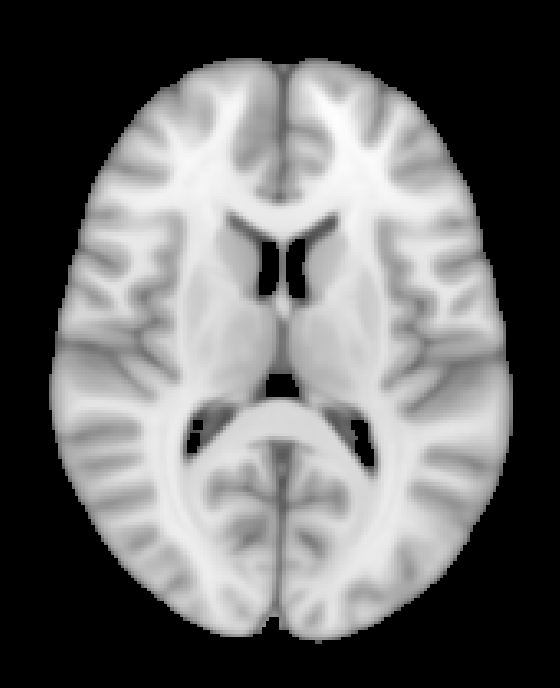
\includegraphics[width = 0.4\textwidth]{mni152.png}
\caption{The MNI-152 standard brain at 1mm resolution. Due to the nature of its construction (which involves averaging across many subjects), structures which are consistently located across subjects (\textit{i.e.}, WM tracts) appear homogenous, whereas regions such as the cortex that are highly variable between subjects are blurred significantly.}
\label{mni152}
\end{figure}

Even when regions of functional correspondence can be established under a conventional volumetric approach, Coalson \textit{et al.} argue that they are ``little more than statistically significant blobs” whose precise relationship to anatomy is uncertain \cite{Coalson2017}. In essence, this situation arises because volumetric registration is performed on the basis of anatomy, but this does not guarantee that areas of function (the ultimate objective) will also align, because the function-anatomy relationship for individual subjects is uncertain. 

Surface-based methods provide an alternative approach. As adopted by the HCP, inter-subject registration can be performed by aligning cortical areas using both folds and `areal' features such as cortical myelin content and resting state networks. Importantly, these features are more closely related within the boundaries of said areas than structural image intensities in volume space \cite{Glasser2016a} or cortical folding patterns \cite{Robinson2014, Robinson2018}. This approach is named multi-modal surface matching (MSMAll) and is able to fuse information from multiple modalities \cite{Robinson2013}. The literature shows there is a clear improvement in the accuracy of inter-subject correspondence of functional areas over volumetric registration under this approach. For example, standard volumetric methods achieved just 35\% of the spatial localisation accuracy of the MSMAll method as used on HCP data \cite{Coalson2017}. A comparison of inter-subject registration based on folding alone versus MSMAll is shown in figure \ref{msmall_demo}.

\begin{figure}[H]
\centering
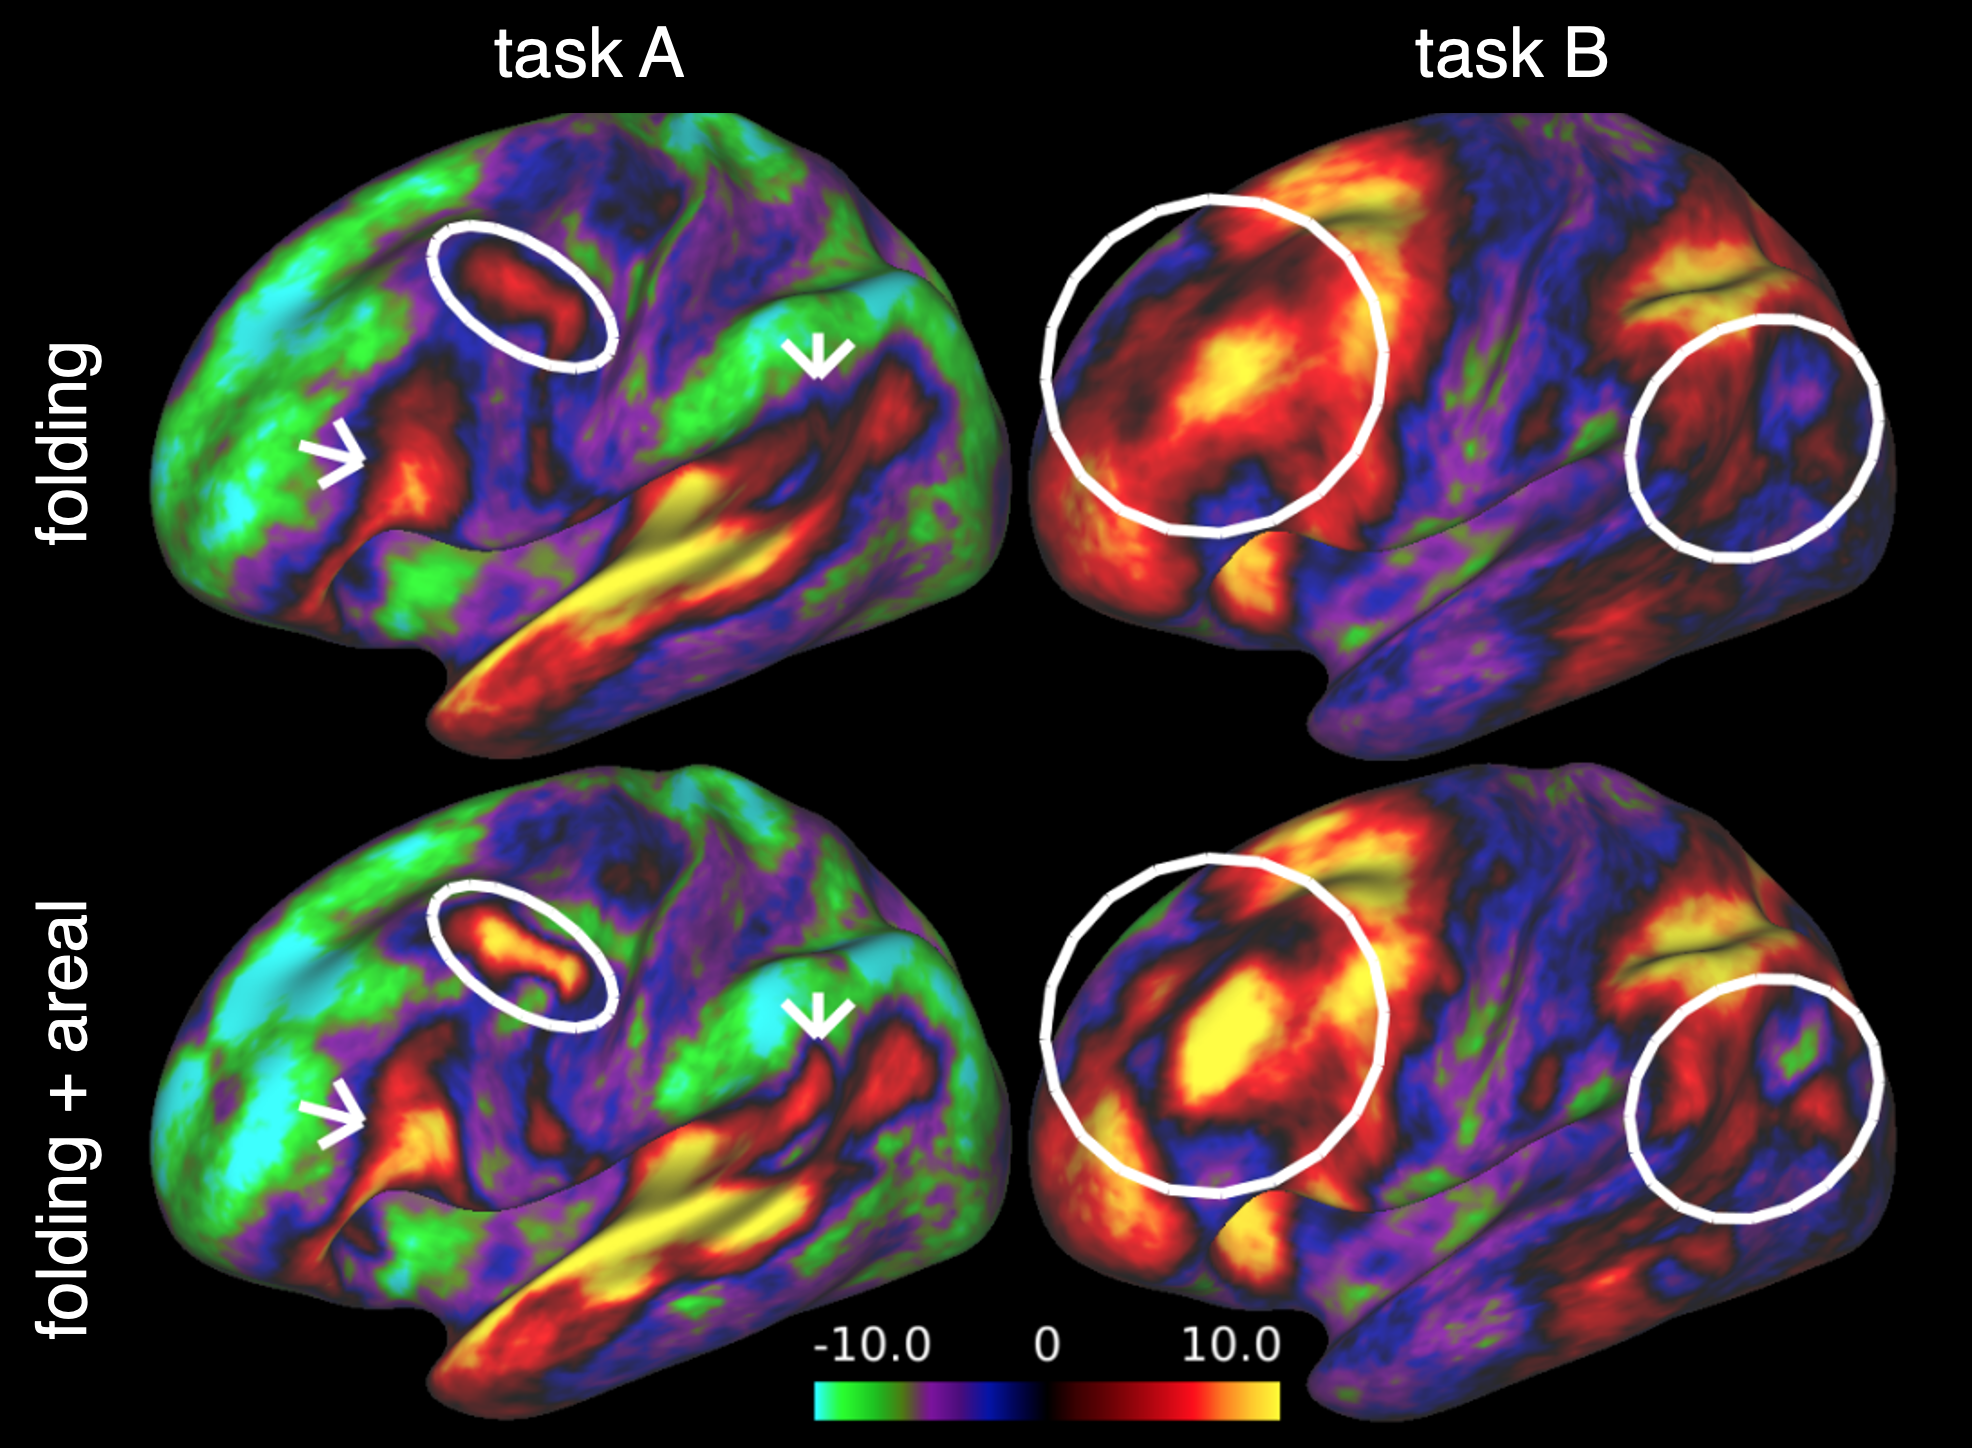
\includegraphics[width = \textwidth]{msmall_demo.png}
\caption{Comparison of surface registration across 120 subjects from the HCP. The top row shows registration based on cortical folding only, whereas the bottom row shows registration based on both folds and areal features (MSMAll). The columns show two different fMRI tasks and the data plotted on the surfaces are the group average $Z$-statistics. MSMAll registration results in increased contrast which is indicative of improved functional correspondence across subjects. Circles and arrows highlight areas of particular difference. Reproduced with permission from \cite{Glasser2016a}.}
\label{msmall_demo}
\end{figure}


\section{Summary}

The aim of this review has been to introduce two broad themes. The first of these, PVE, are an unavoidable consequence of imaging complex anatomies with techniques that have limited spatial resolution. They present an important and widely acknowledged source of confound across multiple modalities and remain a problem for which there is no consensus solution. The importance of this issue is increased when it is desired to study structure and function simultaneously and longitudinally, for example when investigating the structural and physiological changes that accompany brain disease. 

The second theme is the emergence of a surface-based analysis paradigm for the study of the cortex, which has bought about substantial benefits. This is particularly true for large multi-subject studies, for which surface methods offer improved inter-subject registration and localisation of function. Thus far, the focus of such work has been on BOLD and has tended to neglect any signal contribution from the subcortex. Such an approach would not be appropriate for ASL because both the cortex and subcortex produce a signal of interest in their own right. 

Within the context of perfusion measurement in the brain via ASL, a new approach to parameter estimation guided by anatomy could unify these two themes. Firstly, by approaching the problem in an explicitly surface-based manner (as opposed to simply projecting the results of some conventional analysis onto the surface), it may be possible to realise some of the advantages of the surface paradigm for ASL. Crucially, certain aspects of the surface approach would need to be modified for use with ASL, notably, treating signal of interest in the subcortex in an appropriate manner. Logically, this leads towards a requirement for a hybrid surface and volumetric approach that is able to treat the anatomy of both the cortex and subcortex separately. Secondly, as a result of basing the inference on anatomy, PVE are incorporated into the heart of the approach and hence PVEc becomes an intrinsic feature. 

 \newpage 
 \newpage % Activate the following line by filling in the right side. If for example the name of the root file is Main.tex, write
% "...root = Main.tex" if the chapter file is in the same directory, and "...root = ../Main.tex" if the chapter is in a subdirectory.

% !TEX root = ../thesis.tex 

\chapter{The origin and correction of partial volume effects}
\label{pvec_chapter}

\section{Introduction}
\subsection{Interpretations of the partial volume effect}

PVE are a consequence of the limited spatial resolution of physiological imaging data in relation to the length scale of structures of interest. Low spatial resolution arises either due to modality-specific mechanisms (a high PSF in the case of PET), or as a means of mitigating low SNR (in the case of ASL). 

There are multiple possible interpretations of how PVE affect the \DIFdelbegin \DIFdel{acquisition }\DIFdelend \DIFaddbegin \DIFadd{analysis }\DIFaddend of physiological imaging data. One interpretation is that they introduce a dependence between the discretisation basis of the data and the distribution of acquired signal. This is because the signal in a voxel is linearly proportional to the tissue PV within that voxel, and the tissue PVs themselves depend on the voxel grid (according to the intersection made with the structure in question). This is illustrated in figure \ref{CBF_with_PVE_demo}, in which a representative GM CBF map with PVE is simulated by drawing CBF values from a normal distribution and multiplying by a set of ground truth PV estimates. The accompanying scatter plot shows a linear relationship between the PV fraction of a given voxel and its CBF value, a relationship that arises purely due to the discretisation basis of the data. The consequence of this is that any change to the subject anatomy \DIFdelbegin \DIFdel{/ }\DIFdelend \DIFaddbegin \DIFadd{and }\DIFaddend voxel grid intersection (for example, movement during an acquisition) will lead to a change in the PVs associated with said grid, thereby changing the distribution of PVE within the data. To continue the example given in figure \ref{CBF_with_PVE_demo}, this is equivalent to drawing a new set of samples, modulated by the new PVs, from the same underlying parameter distribution.

\begin{figure}
\centering
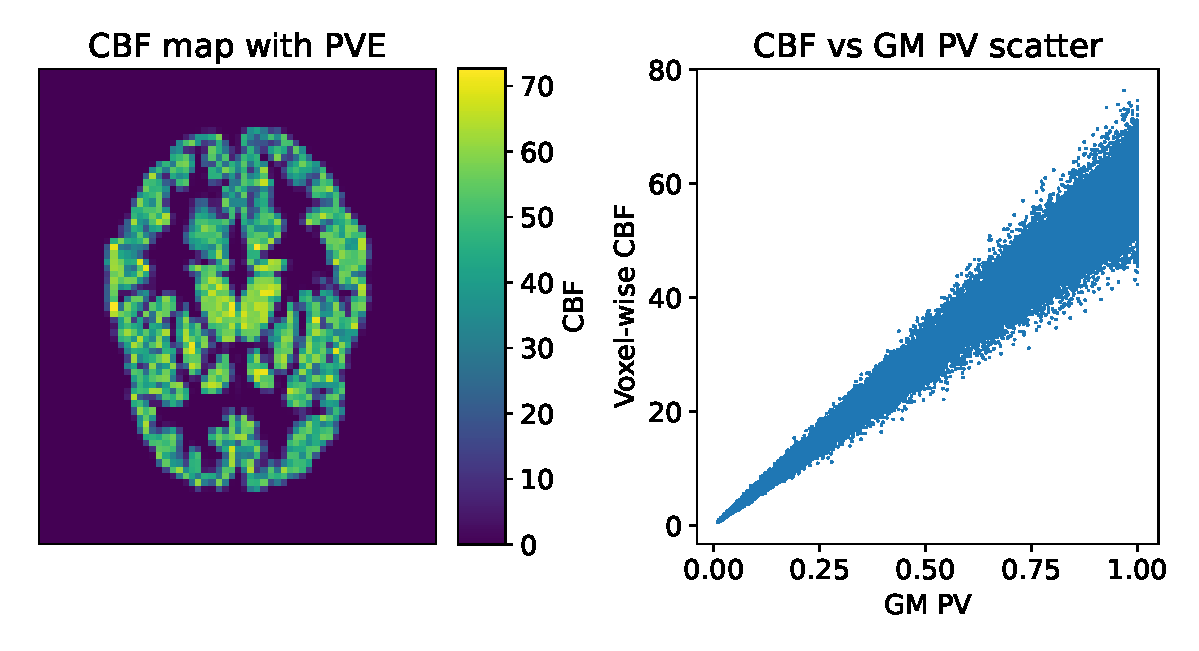
\includegraphics[width = 0.75\textwidth]{CBF_with_PVE.eps}
\caption{Left: \DIFdelbeginFL \DIFdelFL{GM }\DIFdelendFL CBF map \DIFdelbeginFL \DIFdelFL{with }\DIFdelendFL \DIFaddbeginFL \DIFaddFL{for GM }\textit{\DIFaddFL{only}}\DIFaddFL{, incorporating }\DIFaddendFL PVE, simulated by drawing CBF samples from a normal distribution with mean 60 and standard deviation 5. These samples are multiplied with a set of ground truth GM PV estimates to give a representative CBF map \DIFdelbeginFL \DIFdelFL{, as would be obtained from ASL data }\DIFdelendFL for \DIFdelbeginFL \DIFdelFL{example}\DIFdelendFL \DIFaddbeginFL \DIFaddFL{this tissue}\DIFaddendFL . \DIFaddbeginFL \DIFaddFL{An acquired CBF map would include WM CBF as well.  }\DIFaddendFL Right: a scatter plot of voxel PV against CBF value. Even allowing for the variance within the CBF samples drawn from the distribution, a strong relationship between voxel PV and voxel CBF is observed.}
\label{CBF_with_PVE_demo}
\end{figure}

An alternative interpretation of PVE is that they increase the within-class variance of measurements obtained from a given tissue, as illustrated in figure \ref{CBF_PVE_hist_simple}. Once again the same ground truth distribution of GM CBF is assumed, from which CBF maps are simulated using ground truth PV maps at various resolutions (0.7mm, 2.1mm and 3.5mm isotropic). As voxel size increases, it can be seen that the histogram of voxel-wise CBF alters: there are fewer `pure' GM voxels, and hence fewer voxels with high CBF, which leads to greater within-class variance. In quantitative terms, the modal value of the distribution is reduced and variance increased. 

\begin{figure}
\centering
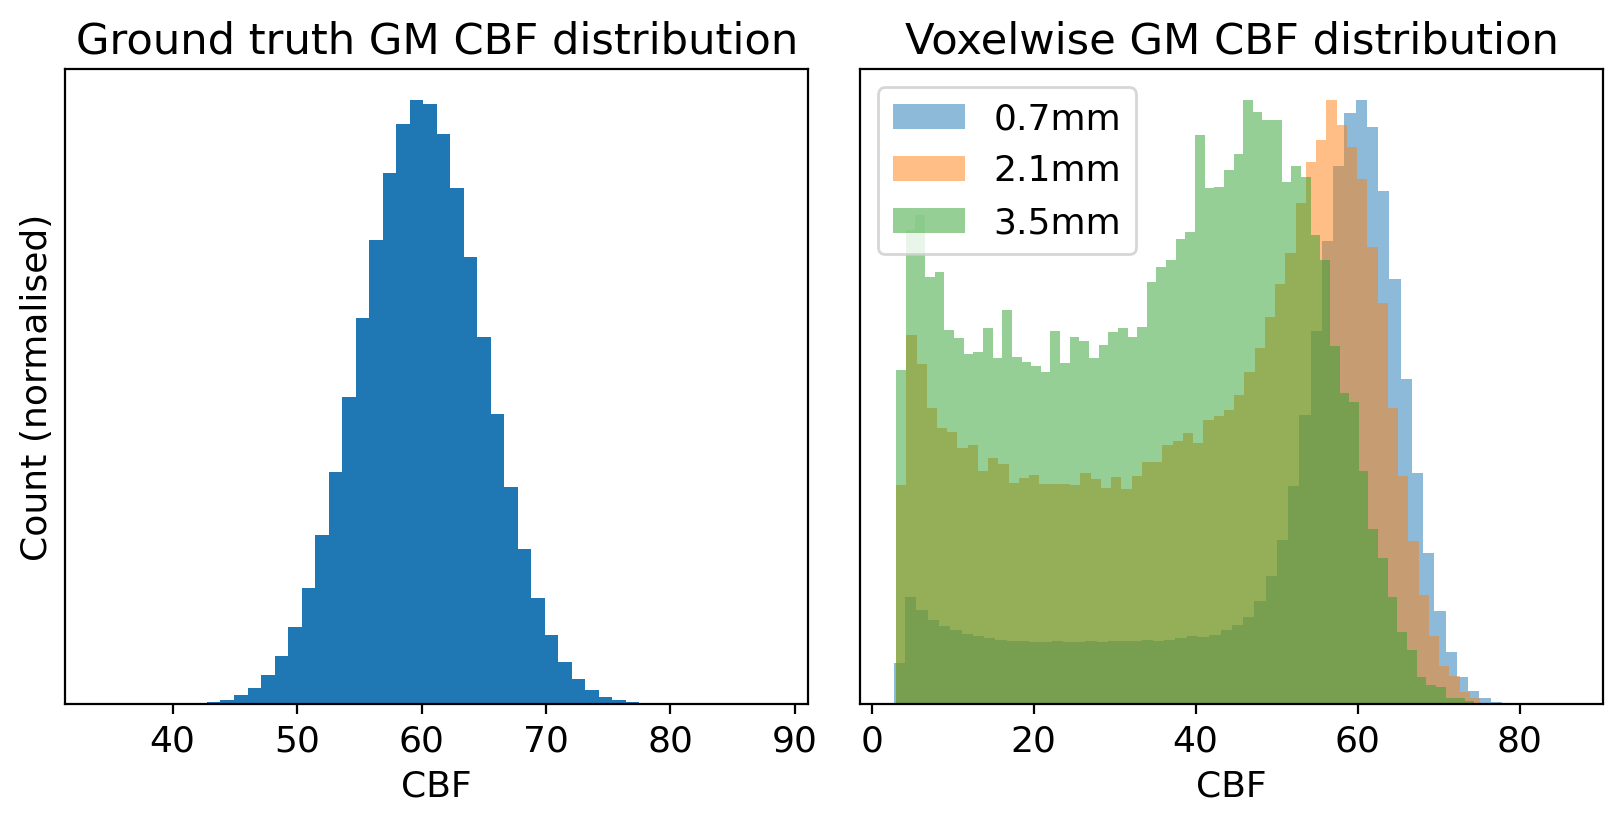
\includegraphics[width = 0.75\textwidth]{CBF_PVE_hists.png}
\caption{Left: a ground truth distribution of GM CBF, normal with mean 60 and standard deviation 5. Samples from this distribution are multiplied with a set of ground truth GM PV estimates at various resolutions to give a representative CBF map, as would be obtained via ASL imaging for example. Right: histograms of voxel-wise CBF at each resolution. As voxel size increases, the histograms become more spread out (within-class variance is increased) and the modal value decreases. The vertical axis has been normalised for clarity.}
\label{CBF_PVE_hist_simple}
\end{figure}

\subsection{The consequences of resampling}

Typical processing pipelines for physiological data make use of motion correction and registration. The former operation is required to combine data from multiple modalities or resolutions (for example, applying a structural ROI from an MRI image to PET data). The latter is desirable to reduce the effects of patient motion during lengthy acquisitions (themselves a means of improving SNR). Both of these operations require resampling, a mathematical operation that is used to transform data between voxel grids.  

Resampling is achieved via the use of high-dimensional interpolation between the coordinates of the voxel grids; in all of the following discussion linear interpolation in three dimensions is assumed (though it is possible to use other basis functions for interpolation, for example splines or sinc functions). Any transformation of a volumetric image may be interpreted as a transformation of the voxel grid upon which the data is currently represented. For example, to translate an image of the brain by 1mm along any axis within a voxel grid, one can hold the brain fixed and shift the voxel grid by 1mm in the reverse direction. Within the image transformation literature, this is often referred to as a \textit{pull} transformation: the forward transformation represented by $T$ may be achieved by applying $T^{-1}$ to the underlying voxel grid. After having determined the new coordinates of the transformed voxel grid, resampling is then used determine the new voxel values. 

The negative consequences of resampling on data quality are well documented. In particular, resampling has the effect of reducing the effective spatial resolution of data, leading to blurring or smoothing artefacts. This follows from the assumption of uniform signal distribution that is necessary for interpolation. Figure \ref{resamp_demo} provides an illustrative example: a structure boundary is shown in purple, \DIFaddbegin \DIFadd{and }\DIFaddend a voxel grid before and after transformation is shown in red and blue respectively. The dashed side of the boundary denotes the interior of the structure. 

\begin{figure}
\centering
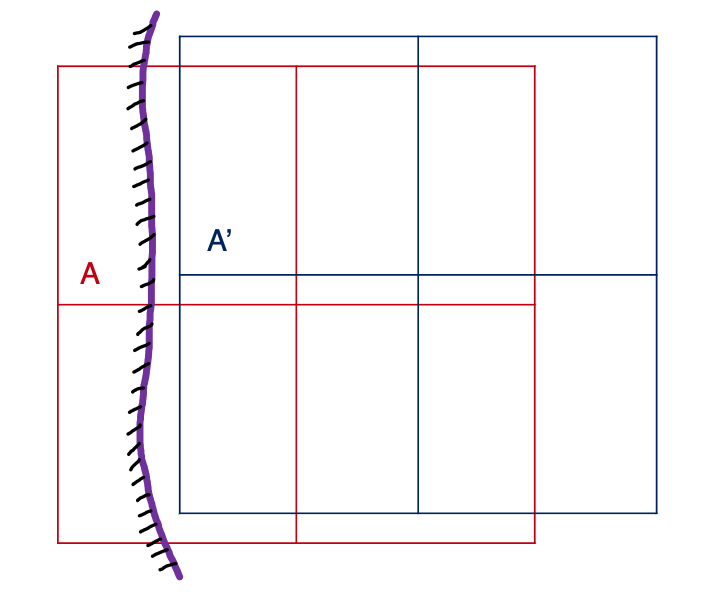
\includegraphics[width = 0.6\textwidth]{resamp_demo.png}
\caption{Illustration of subvoxel effects, caused by the ambiguous position of a structure boundary within a voxel before and after resampling. Due to the application of some transformation, the voxel grid shifts from red to blue; voxel $A$ becomes voxel $A'$. A structure boundary is shown in purple, with the dashed side as the interior, so voxel $A$ is approximately 30\% interior and 70\% exterior. After resampling, $A'$ overlaps significantly with $A$, so will be assigned a similar value to it, even though it does \textit{not} intersect the structure at all. This arises due to the assumption of uniform signal distribution within voxels, which is anatomically incorrect.}
\label{resamp_demo}
\end{figure}

The voxel labelled $A$ is transformed to $A'$. Prior to transformation, voxel $A$ contains PVs caused by the partitioning of the voxel by the structure boundary (approximately 30\% interior and 70\% exterior). The signal in voxel $A$ will therefore be a mixture of interior / exterior signals in proportion to the PVs. After application of the transformation, it is necessary to evaluate the new signal for voxel $A'$. Because of the significant overlap between voxel $A$ and $A'$, the resampled value for $A'$ will be strongly weighted towards $A$ (the exact weighting is determined by the interpolation function used; but in any case $A$ will contribute substantially). As a result, the resampled value for $A'$ will contain a non-zero proportion of signal from the interior of the structure. This is despite the fact that voxel $A'$ does not actually intersect the structure at all, so the correct solution for $A'$ would not contain any signal from the structure. 

The above situation arises due to the assumption of uniform signal distribution that is made during interpolation. The interpolated value for a voxel is evaluated as a weighted average across neighbouring voxels, where the weights are determined by the relative distances of these neighbours. Importantly, the operation is blind to the distribution of signal \textit{within} those neighbours, and specifically the fact that they may contain PVs, because there is no finer discretisation of the data available. As there is no basis for determining which signal contributions within the neighbours should or should not be included in the output, the assumption of uniform distribution is instead made, leading to an artificial increase in PVE in the output. This mechanism - the lack of information about spatial distribution of signal within a voxel - is hereafter referred to as the \textit{subvoxel effect}. A practical example of the impact of the subvoxel effect on a structural T1w image is shown in figure \ref{translate_data}. 

\begin{figure}
\centering
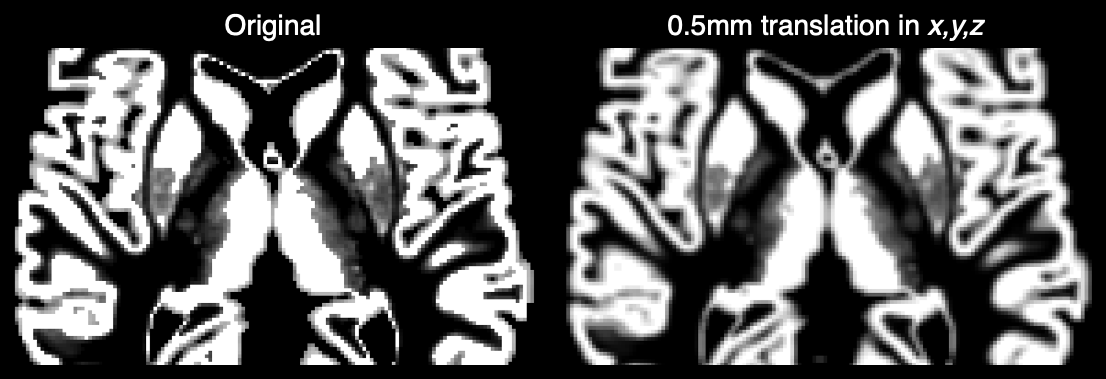
\includegraphics[width = \textwidth]{translate_data.png}
\caption{Effect of resampling on a GM PV map at 1mm resolution. The original map is shown on the left, the application of a 0.5mm translation in each axes is shown on the right. Due to the ratio of translation distance (0.5mm) to voxel size (1mm), subvoxel effects are maximised; a significant loss in edge definition is observed after resampling.}
\label{translate_data}
\end{figure}

It is difficult to quantitatively measure the impact of resampling on PVE. To do so would require the ability to express some volumetric ground truth data in an arbitrary voxel grid without making use of resampling, otherwise a trap of circular reasoning results. Such an analysis can however be performed using simulations. In particular, by using simulated surfaces to represent structure boundaries, it is possible to calculate PVs in any arbitrary grid to a high precision via a numerical method. The impact of resampling may then be quantified by performing a comparison between i) direct evaluation of PVs in an arbitrary voxel grid using the numerical method, and ii) evaluation of PVs in a high resolution voxel grid using the numerical method followed by resampling into the same arbitrary grid. For example, PVs can be obtained in a 3mm voxel grid either by direct evaluation of the numerical method in that grid, or by evaluating PVs in a 1mm grid and then resampling them to the lower resolution. Figure \ref{resamp_ratio} shows the results of such an analysis, applied to the simulated surfaces representing cortical anatomy that will be detailed later in section \ref{tob_sim_surfaces}. 

\begin{figure}
\centering
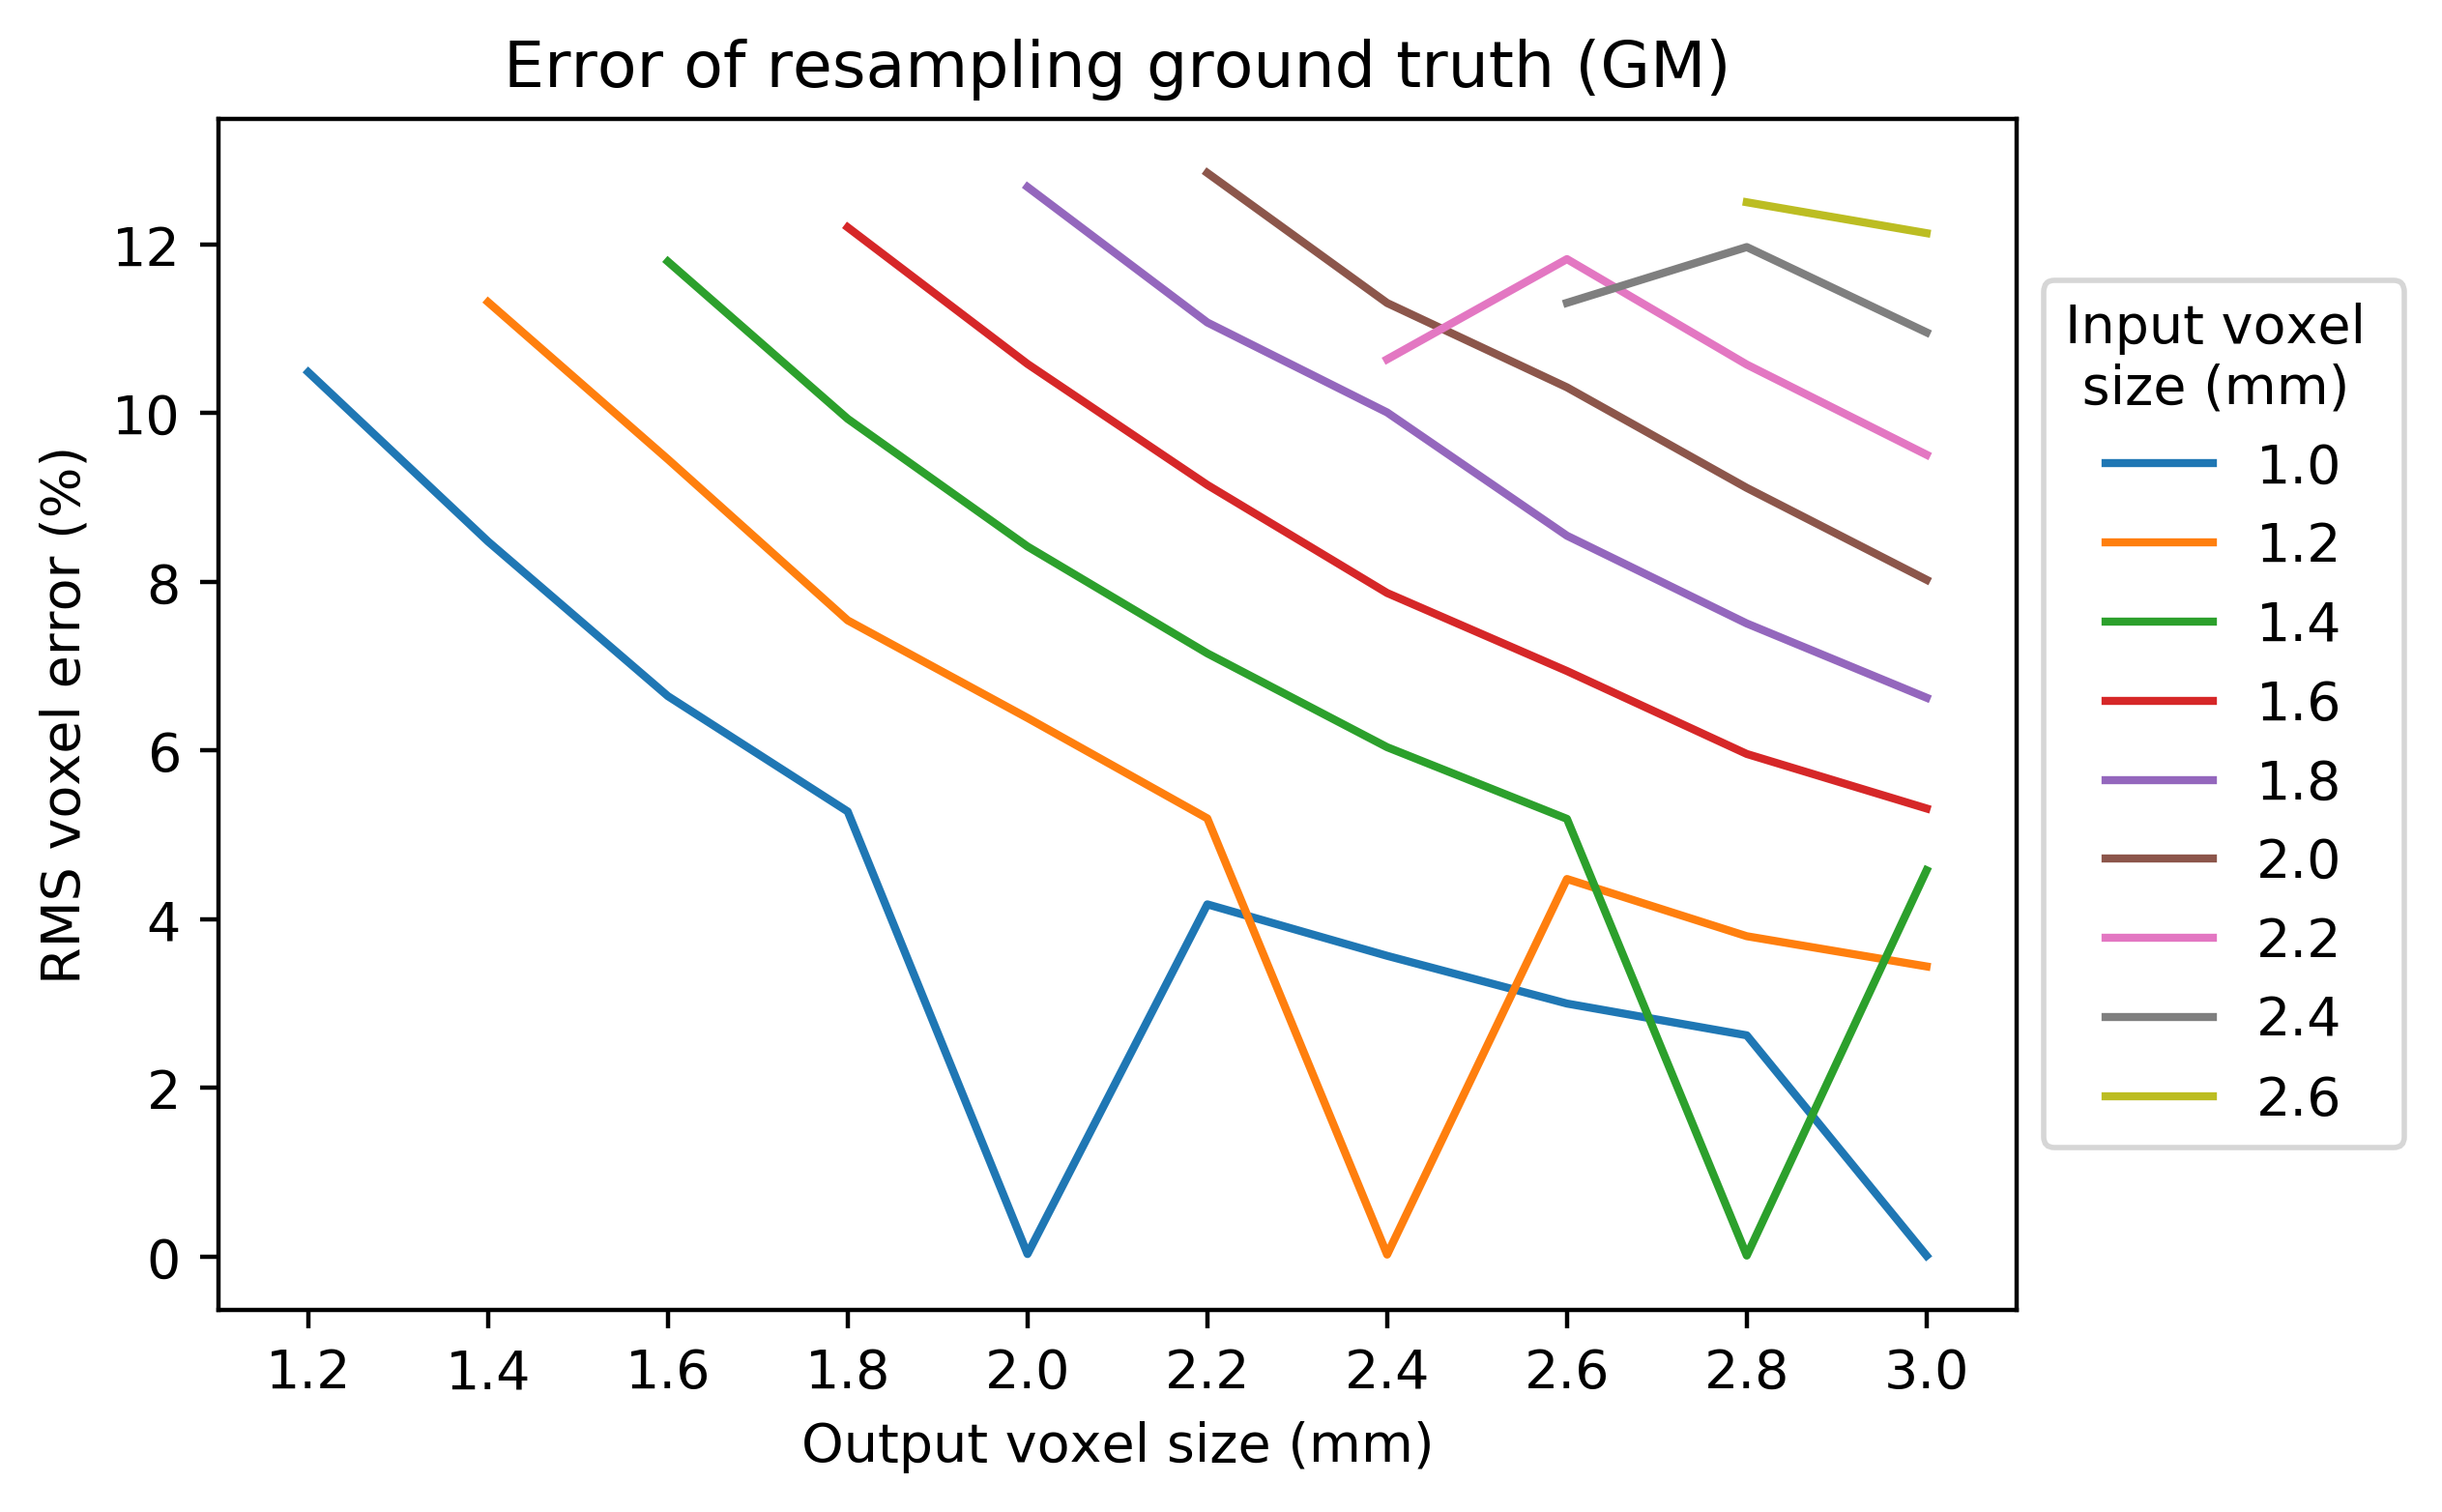
\includegraphics[width = 0.7\textwidth]{resamp_ratio.png}
\caption{Error associated with resampling a PV map as a function of input and output voxel size, masked to consider only voxels containing PVs. At each resolution, PVs were calculated either by i) direct evaluation of a numerical method, or ii) resampling the results of the numerical method \textit{from a smaller voxel size}. In general, the error due to resampling decreases as the ratio of output to input voxel size increases. When this ratio takes an integer value, the error can disappear completely, but this is due to the perfect alignment of voxel grids within this simulation.}
\label{resamp_ratio}
\end{figure}

Each trace on the plot represents a different input voxel resolution at which ground truth PVs were evaluated. These ground truth maps were then resampled to all resolutions above the input (for example, the 1.4mm truth was resampled to 1.6, 1.8, ... \textit{etc}), and the root mean square (RMS) voxel error with respect to ground truth evaluated (masked to consider only voxels that contain PVs on the ground truth). Multiple trends were seen: firstly, as the input voxel size increased, error at all output voxel sizes increased. Secondly, as the ratio of output to input voxel size increased, the error decreased. Finally, the error fell to zero when this ratio took an integer value. This was due to the use of perfectly aligned voxel grids for these simulations, which in turn meant that each large voxel corresponded perfectly to a grid of $N$ smaller voxels on the input data (where $N$ is the ratio of voxel sizes). The significance of an integer ratio of voxel size is that subvoxel effects are eliminated: the input voxel is entirely contained within a single output voxel, so the assumption of uniform signal distribution is of no consequence. Hence, this analysis demonstrates that resampling has the effect of further mixing, or increasing, whatever PVE may already be embedded within data. 


\subsection{Implications for PVEc} 

Given that resampling further increases the PVE embedded within data, it is logical to question whether this will have implications for the successful application of PVEc. This is especially pertinent for analysis strategies that do not operate in native acquisition space. For example, the analysis paradigm adopted by some SPM (a neuroimaging software package) and HCP pipelines places an emphasis on the immediate transformation of raw data into MNI space, though it is important to note that PVE are less of a challenge for the modality these pipelines are designed for (BOLD) \cite{Glasser2013, Friston2003a}. 

This question also applies to the analysis of repeated acquisitions of the same subject. A frequently cited theoretical justification for PVEc is that it can improve the repeatability of parameter measurements by removing the dependence of voxelwise measurements on tissue PV. This is necessary because PVs are acquisition-specific, arising due to the particular interaction of subject anatomy with an imaging matrix at the exact moment of acquisition. Due to subject motion, for example, the embedding of PVE across repeats cannot therefore be assumed to be constant. 

This poses a challenge for any analysis that requires spatial correspondence across repeats. Consider, for example, co-registration of repeat ASL data into alignment with a structural image at original voxel resolution. Assuming perfect registration and constant perfusion across the repeats, signal from any given location within the brain should in theory end up in the same voxel in common analysis space, and therefore that voxel should have the same value across all repeats. In practice, the PVE that were embedded within the repeat data were different, and therefore this voxel in common space will have different values across the repeats. The justification for performing PVEc is immediately clear; removing the differing embeddings of PVE within the repeat data should reduce variability of measurements between repeats. The challenge is in determining \textit{what} PV estimates should be used for the correction. 

The obvious approach would be to use PV estimates obtained from a segmentation of the structural image. This is made simpler by the fact that the common analysis space is already in alignment with the structural image, so all that is required is a downsampling with identity transformation of the PV estimates in the structural grid to the ASL grid. The schematic for such a strategy is illustrated in figure \ref{rpt_paradox} and is hereafter referred to as the \textit{naive} approach. Nevertheless, this approach is somewhat paradoxical: \textit{one} single set of PV estimates are used to correct \textit{all} of the repeat data, despite the fact that the PVE within each are expected to be different. It therefore follows that this strategy for PVEc will lead to sub-optimal outcomes. 

\begin{figure}
\centering
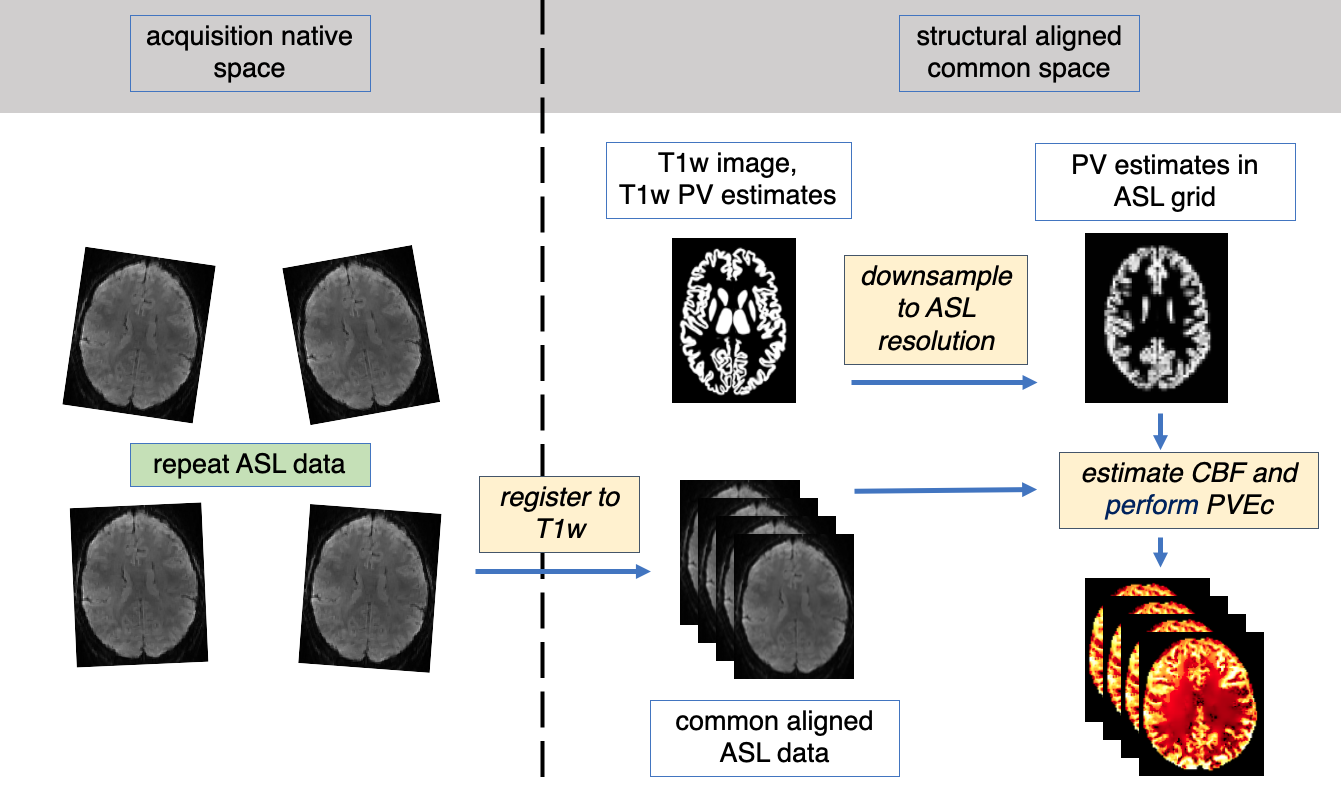
\includegraphics[width = \textwidth]{rpt_paradox.png}
\caption{The paradox of PVEc in a common analysis space for repeat data. The point of origin is highlighted in green. The ASL repeats are co-registered into a common analysis space, and then PVEc is performed using a single set of PV estimates downsampled from structural resolution for all repeats. This is despite the fact that theoretical understanding of PVE suggests each individual repeat will contain \textit{different} PVE.}
\label{rpt_paradox}
\end{figure}

What is instead required are a set of PV estimates for each repeat that convey information about the PVE that held true \textit{at the time the data was acquired}. These can readily be obtained by reversing the transformation between the native ASL data and the structural image, so that the T1w PV estimates are transformed and downsampled into the native voxel grid of the ASL data. Thereafter, the same set of transformation operations that are required to move the repeat data into common space are simultaneously applied to the native space PV estimates. This means that whatever extra PVE are introduced into the data by resampling are also introduced into the PV estimates themselves. In effect, the PVs that held true at the time of acquisition are updated to incorporate the extra PVE that are introduced by resampling. Because this strategy involves the use of two resampling operations for the PV estimates (firstly, from structural space to ASL native space, and then from ASL space to the common analysis space), this strategy is referred to as the \textit{double-resampling} approach, the schematic of which is illustrated in figure \ref{dbl_paradox}. The amount of PVE introduced by the two resampling operations will be very different. The resampling from structural to native ASL space introduces little PVE (subvoxel effects are minimal because the ratio of output to input voxel size is greater than unity), whereas the resampling from native ASL space to the common analysis space introduces high PVE (the ratio of output to input voxel size is unity). 

\begin{figure}
\centering
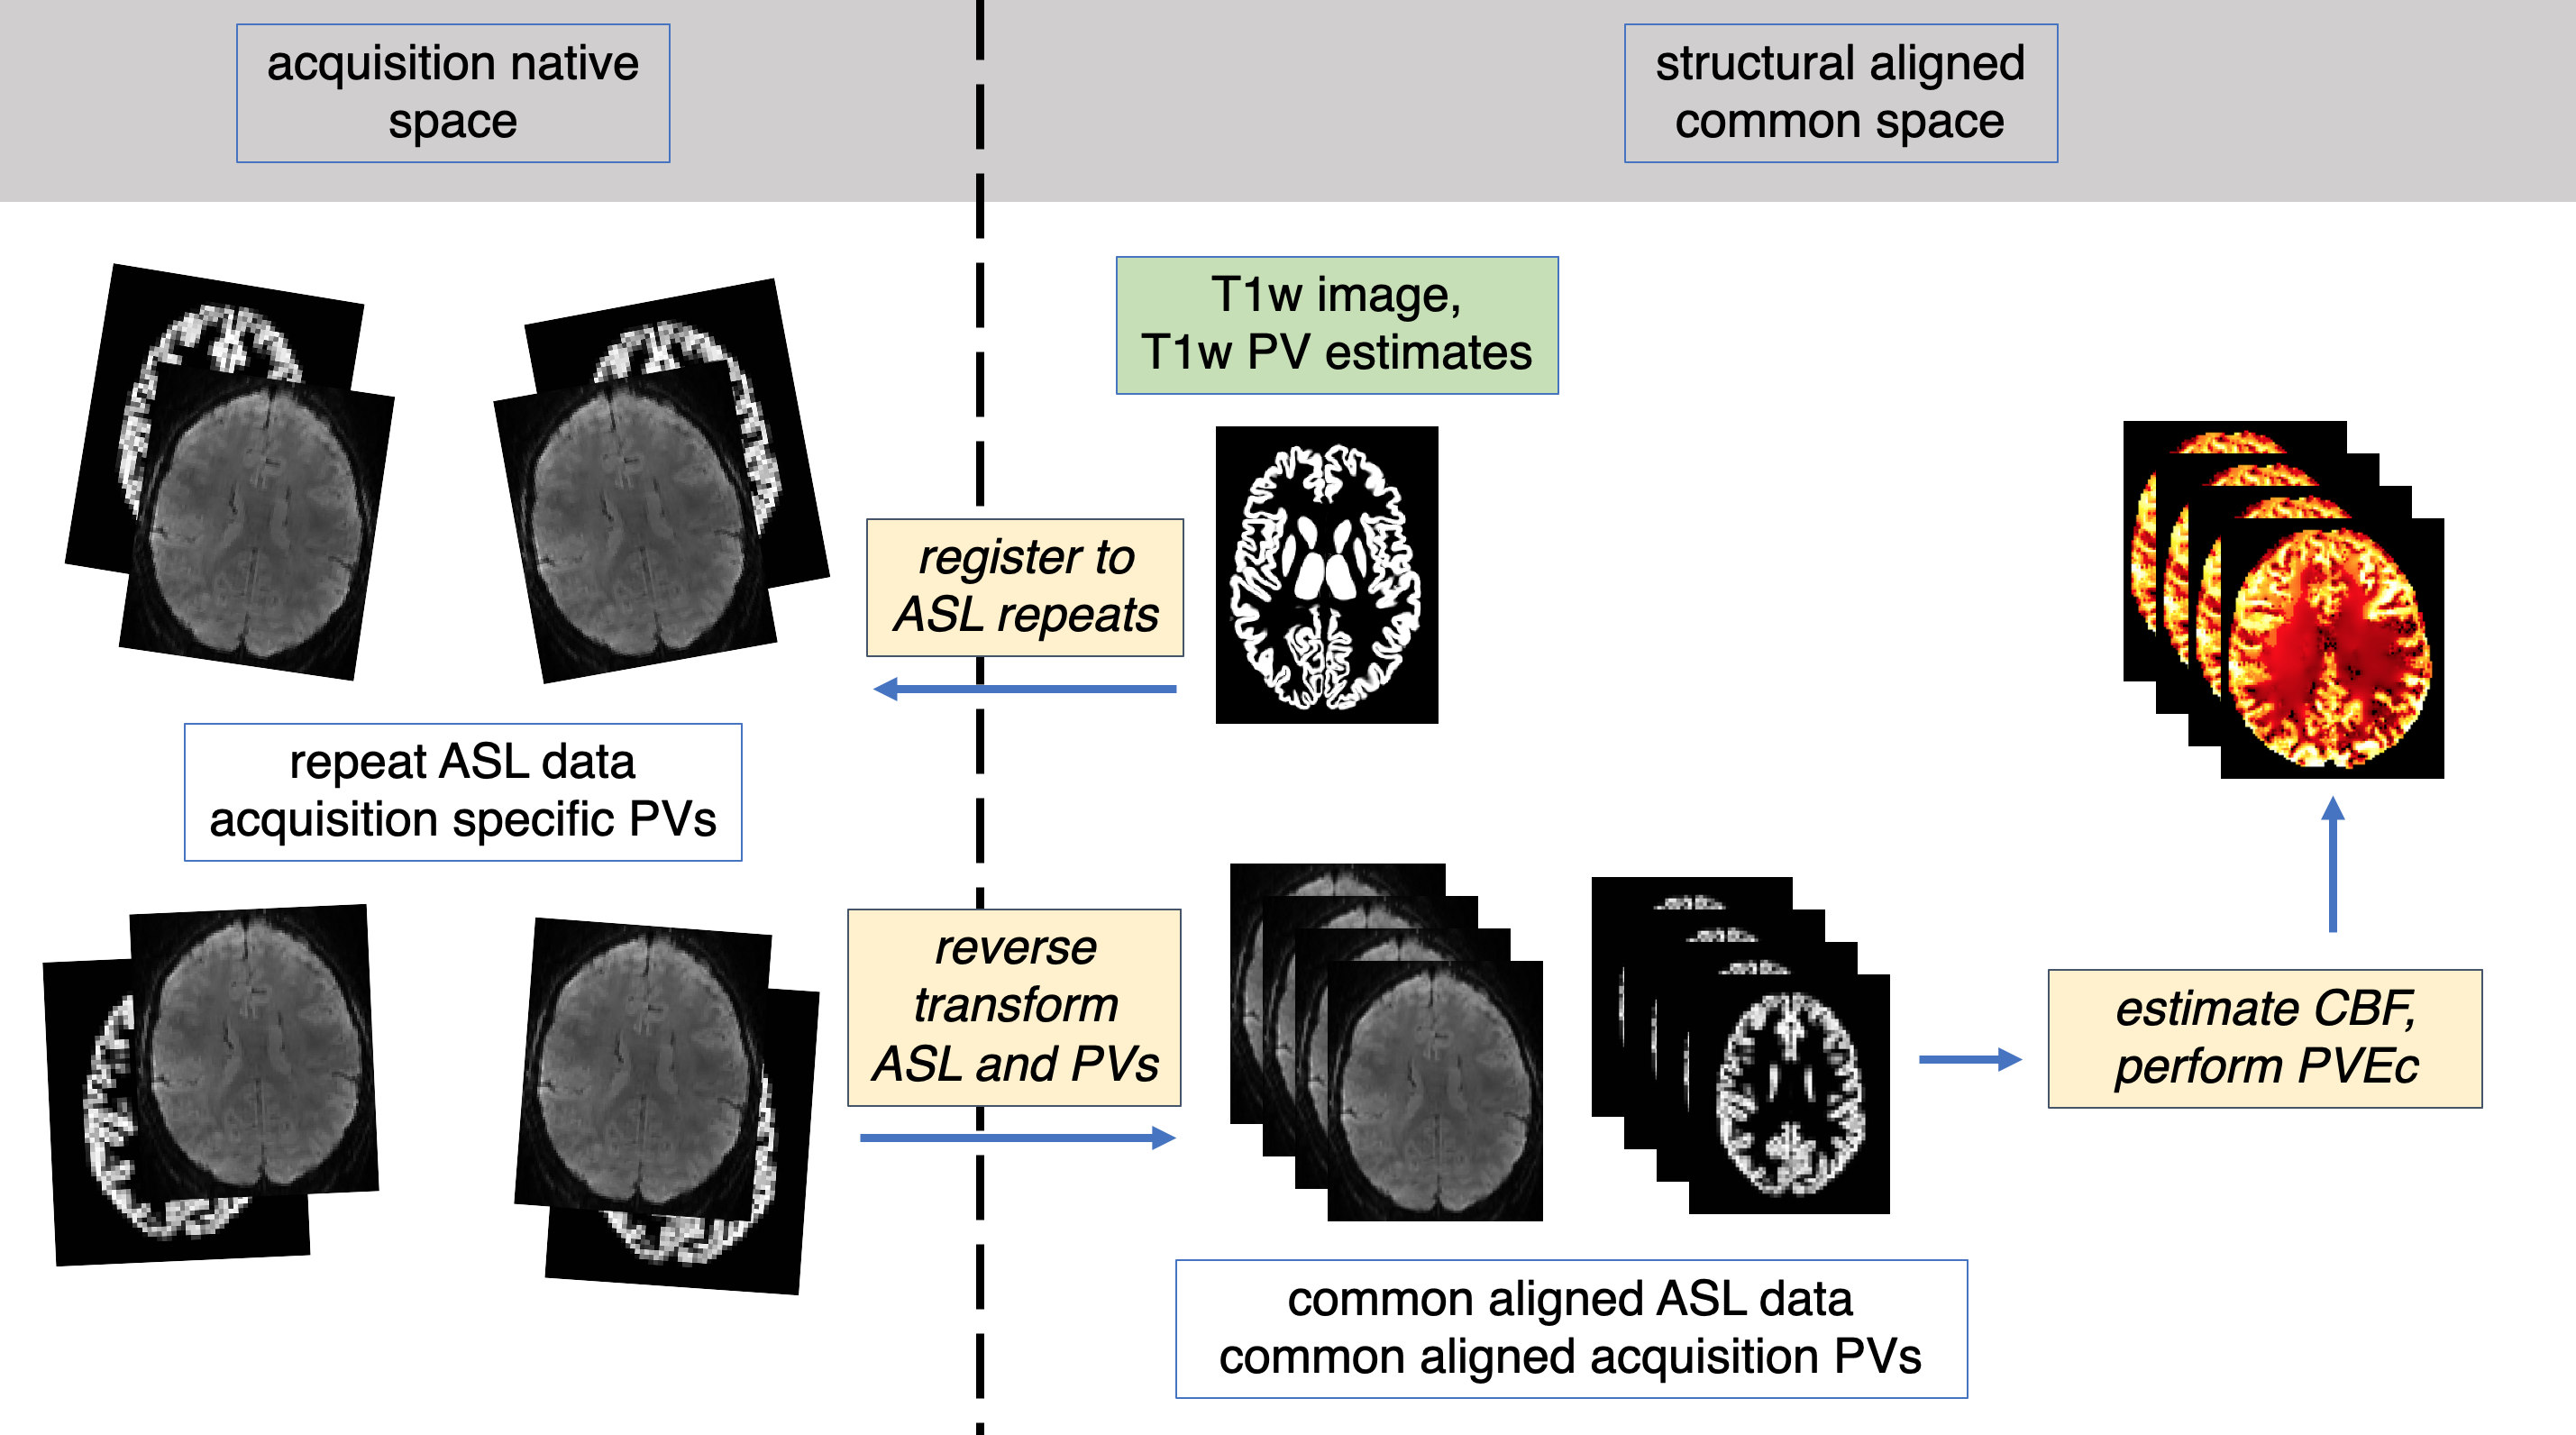
\includegraphics[width = \textwidth]{dbl_paradox.png}
\caption{The double-resampling strategy for PVEc of repeat data in a common analysis space. The point of departure is highlighted in green. PVs are first estimated in the native space of each repeat acquisition, and then undergo the same set of transformations into common space. This results in a unique PV map used for the correction of each repeat in common space, which better matches theoretical understanding of the origin of PVE.}
\label{dbl_paradox}
\end{figure} 


\subsection{Experimental hypothesis}
The hypothesis investigated in this chapter is that the consequences of resampling are substantial enough to negatively impact the application of PVEc. The corollary of this is that, if PVE are to be minimised, analysis in the native space of the data should always be preferred (though there may of course be other reasons to perform analysis in a non-native space). Finally, it is hypothesised that if estimation in a non-native space is required, then the double-resampling strategy for obtaining PV estimates outperforms the naive strategy. These hypotheses have been investigated using simulated and \textit{in-vivo} ASL data. 

\section{Datasets}

\subsection{Terminology}

The following terminology is hereafter used. \textit{Original, acquisition} or \textit{native} space data refers to ASL data in the same voxel grid and alignment as that in which it was simulated or acquired; \textit{i.e.}, data that has not been processed in any way. \textit{Resampled} data refers to data that has been through a resampling process, potentially involving a transformation into different alignment, and \textit{common space} data refers to data has been transformed and resampled into alignment with some external reference for the purpose of establishing spatial correspondence between repeat acquisitions. For all the analyses presented herein, \textit{common space} was defined in alignment with the subject's anatomical image at the same voxel size as the native ASL data. 

PVEc was always performed with partial volume estimates that were in alignment with the ASL data. The only variable in the process was the amount of resampling that had been applied to the PV estimates: \textit{naive} refers to PV estimates obtained via the shortest possible path (\textit{e.g.}, direct downsampling from structural resolution), whereas \textit{resampled} refers to naive estimates that have been through the same set of resampling operations as the ASL data itself. Finally, in the context of repeat data in a common analysis space only, \textit{double-resampled} means naive PVs that have been transformed into the acquisition space of the \DIFdelbegin \DIFdel{ASL data}\DIFdelend \DIFaddbegin \DIFadd{individual ASL repeats}\DIFaddend , and then reverse-transformed back into the common analysis space alongside the \DIFdelbegin \DIFdel{ASL data itself}\DIFdelend \DIFaddbegin \DIFadd{repeats themselves}\DIFaddend . This is a round-trip transformation resulting in no change in the alignment of the PV estimates\DIFdelbegin \DIFdel{themselves}\DIFdelend , but extra PVE will be \DIFdelbegin \DIFdel{introduced }\DIFdelend \DIFaddbegin \DIFadd{present in the data }\DIFaddend due to the \DIFaddbegin \DIFadd{two }\DIFaddend resampling operations.

\subsection{Simulated data}
\label{pvec_chapter_sim_data}

Simulated ASL data was produced using structural pre-processed data for subject 103818 from the HCP \cite{Glasser2013}. Surface segmentations of the cortex and subcortex for this subject were processed to yield a reference set of PV estimates using the surface-based method detailed in chapter \ref{tob_pv_chapter}. The ASL signal was calculated using the \textit{aslrest} model included with FSL FABBER \cite{Chappell2009} for pure GM and WM respectively and then combined in linear proportion using the PV estimates. As FABBER was also used for perfusion estimation, this implies that in the idealised case it should be possible to perfectly recover ground truth parameter values from the simulated data. The simplifying assumption of constant CBF and ATT in both GM and WM was made. Typical values of 60, 20 ml/100g$\cdot$min and 1.3, 1.6s were used for GM and WM respectively. The assumption of constant CBF and ATT is helpful because it means that any within-tissue variance in the data must be explained by PVE, which in turn means the efficacy of PVEc can be assessed by observing reductions in within-tissue variance of the output parameter distributions. Other simulation parameters were as follows: pcASL of 1.8s label duration with 5 PLDs (0.75, 1.0, 1.25, 1.5, 1.75, and 2.0s) and 8 repeats at each PLD (a total of 48 label-control pairs). 

One timeseries was simulated with high SNR in order to provide an insight into the PVE/resampling interaction in the absence of `real-world' confounds. SNR was defined via 

\begin{equation}
\label{snr_defn}
\mathrm{SNR} = \frac{s \sqrt(n)}{\sigma}
\end{equation}

where $s$ represents maximum signal in pure GM, $n$ is the number of volumes in the timeseries, and $\sigma$ is the standard deviation of noise. When applying this relation to \textit{in-vivo} data, $s$ may be approximated by taking the maximum timeseries-mean of the data. With the aforementioned sequence parameters, $s$ was 45 arbitrary units (a.u.) at 1.5s PLD. Zero-mean white noise was added to the data to yield an SNR of 27. 

Four repeat timeseries were simulated with low SNR to realistically model the challenges of working with \textit{in-vivo} data. Using the same definition of SNR and maximum signal value (45 a.u. at 1.5s PLD), zero-mean white noise was added to the data to yield an SNR of 9. In order to simulate the effects of patient motion during a scanner session, the low SNR repeats were each produced in their own `acquisition-specific' alignment. This was achieved by applying four random affine transformations to the reference PV estimates to produce acquisition-specific PV maps, from which the ASL data was simulated. Finally, the reverse transforms were applied to the ASL data to bring them back into alignment with the reference PV estimates in common space. The transformations were generated by concatenating rotations around the $z$ and $x$ axis with a translation along each axis; the rotations were drawn from the uniform integer distribution between [0, 5] degrees and the translation components in $xyz$ were drawn from the uniform continuous distribution between [0, 6]mm. This process is illustrated in figure \ref{simrpt_schema}. 

\subsection{\textit{In-vivo} data}

\textit{In-vivo} data was acquired for two subjects at 7T using a single TI pASL sequence. For the first subject, one timeseries of 200 volumes was obtained (referred to as the `high SNR' data); for the second subject, three timeseries of 100 volumes were obtained in the same session (referred to as the `low SNR repeats'). Other sequence parameters were as follows: QUIPSS-II labelling of 700ms bolus duration, 1.8s TI, 1.5mm isotropic voxel size on an imaging matrix of 128 x 128 x 36 and 2D EPI readout with 0.0325s slice acquisition time. \DIFaddbegin \DIFadd{Further details are given in appendix \ref{7T_appendix}. }\DIFaddend The data was then downsampled without interpolation to 3mm isotropic voxel size by summing over 2x2x2 voxel grids to increase PVE and improve SNR. Using the definition of SNR given in equation \ref{snr_defn}, the SNR of the repeats after this processing was estimated to be around 9. \DIFaddbegin \DIFadd{ASL data is conventionally acquired at 3T; 7T data was used in this work as it permitted a higher image resolution which in turn reduced the levels of PVE naturally present in the data, which was assumed to make it easier to observe the impact of resampling on PVE. Data acquisition for this work started in February 2020 and was interrupted by the spread of Covid-19. 
}\DIFaddend 

Structural T1w MP2RAGE images were obtained at 0.7mm isotropic resolution for both subjects and processed using FreeSurfer and FSL FIRST to obtain surface segmentations. The surface-based method detailed in chapter \ref{tob_pv_chapter} was then used on these to obtain PV estimates. All registration between ASL and structural data was performed using FSL FLIRT (including \DIFdelbegin \DIFdel{MCFLRIT }\DIFdelend \DIFaddbegin \DIFadd{MCFLIRT }\DIFaddend for motion correction) with six degrees of freedom \cite{flirt}\DIFaddbegin \DIFadd{, though resampling operations (application of the registrations) was performed using a separate software package (see section \ref{pvec_resamp_perf_methods})}\DIFaddend . 

\section{Methods}

\subsection{Perfusion quantification and PVEc}
\DIFaddbegin \label{pvec_resamp_perf_methods}
\DIFaddend 

Two forms of PVEc were investigated: Asllani's LR method \cite{Asllani2008} and the spatially regularised mode incorporated within BASIL \cite{Chappell2009, Chappell2011}. The LR method can be applied to either ASL data itself, or uncorrected  CBF and ATT maps resulting from a non-PVEc run. The former variant (`LR on data') was used for this work as it better preserves the differing dynamics of perfusion for each tissue with multi-PLD data. This was achieved by performing the regression on each volume of the ASL timeseries to yield two separate timeseries for GM and WM. FSL BASIL was then run on each output timeseries independently in non-PVEc mode (with tissue properties fixed for GM or WM as appropriate). A 3x3x3 kernel including cardinal neighbours only (a total of six neighbours per voxel) was used. It is well-documented that the LR method provides a relatively high and fixed level of smoothing to data, but the extent of smoothing does not depend on the data itself (and is fixed instead by the kernel size) \DIFaddbegin \DIFadd{\mbox{%DIFAUXCMD
\cite{Asllani2008, Zhao2017a}}\hspace{0pt}%DIFAUXCMD
}\DIFaddend . 

The spatially-regularised PVEc built into BASIL is conceptually similar to the LR approach in that it also uses a kernel of neighbouring voxels in order to separate signal into GM and WM contributions. The key difference is that the weight given to the kernel (the spatial precision) is a parameter of the VB inference process that is optimised; it therefore provides adaptive spatial smoothing in a data-driven manner that has been shown to better preserve details than the LR method \cite{Zhao2017a}. A crucially important aspect of spatially-regularised BASIL is that it makes use of a Laplacian spatial prior to condition the under-determined system of equations that arise due to PVE in each voxel neighbourhood. It \textit{also} makes use of the spatial prior as a means of mitigating the low SNR commonly seen in ASL data. This dual use of the spatial prior - as a means of reducing noise, and as a means of implementing PVEc - means it is difficult to quantitatively compare the amount of smoothing that it deems optimal across different datasets, or that it deems optimal for PVEc versus non-PVEc. This is in contrast to the LR method for which the amount of smoothing is a fixed property of the regression kernel.

For both variants of PVEc on simulated data, both CBF and ATT were estimated. All tissue and model properties were left at their default BASIL values (the same used when simulating the data). 

For the \textit{in-vivo} data, the following BASIL settings were used to estimate CBF only (both variants of PVEc were used). ATT was fixed at the reference value of 1.3s or 1.6s for GM and WM respectively, the T1 value of blood at 7T was set at 2.1s and the pASL labelling efficiency was set at 0.95 \cite{Zhang2013}. Slice time correction of 0.065s was used and the calibration was performed in a voxelwise manner. 

All transformation, resampling and interpolation operations were performed using the \textit{regtricks} software package \cite{regtricks} with trilinear interpolation and intermediate supersampling (the same approach used by FSL \textit{applywarp}). Although \DIFdelbegin \DIFdel{other interpolating basis functions }\DIFdelend \DIFaddbegin \DIFadd{higher order interpolating functions such as splines }\DIFaddend can reduce the loss in spatial resolution associated with resampling, trilinear interpolation remains in \DIFdelbegin \DIFdel{very }\DIFdelend common usage, particularly for low resolution data \DIFdelbegin \DIFdel{. 
}\DIFdelend \DIFaddbegin \DIFadd{where splines may introduce extra artefacts. The use of trilinear interpolation in this work may thus be regarded as a comparison to the worst-case scenario (though one which is by no means uncommon); the use of splines would likely reduce but not eliminate the impact of resampling. 
}\DIFaddend 


\subsection{Simulated data}
\label{pvec_simulation_data_section}

In order to investigate the effect of resampling on PVE in the absence of any other effects, the high SNR data was taken through a round-trip of resampling. A random affine transformation (generated in the same manner as for the simulated repeats) was applied to the data to forward-transform it, followed by a separate application of the reverse transform. This resulted in data that had been through two rounds of resampling but remained in its original alignment. The PV estimates were also taken through the same round-trip, CBF was estimated from both the original and resampled data, and finally PVEc was performed using both the naive (original) and resampled PV estimates. The schematic for this is illustrated in figure \ref{doublesim_schema}. 

\begin{figure}[h]
\centering
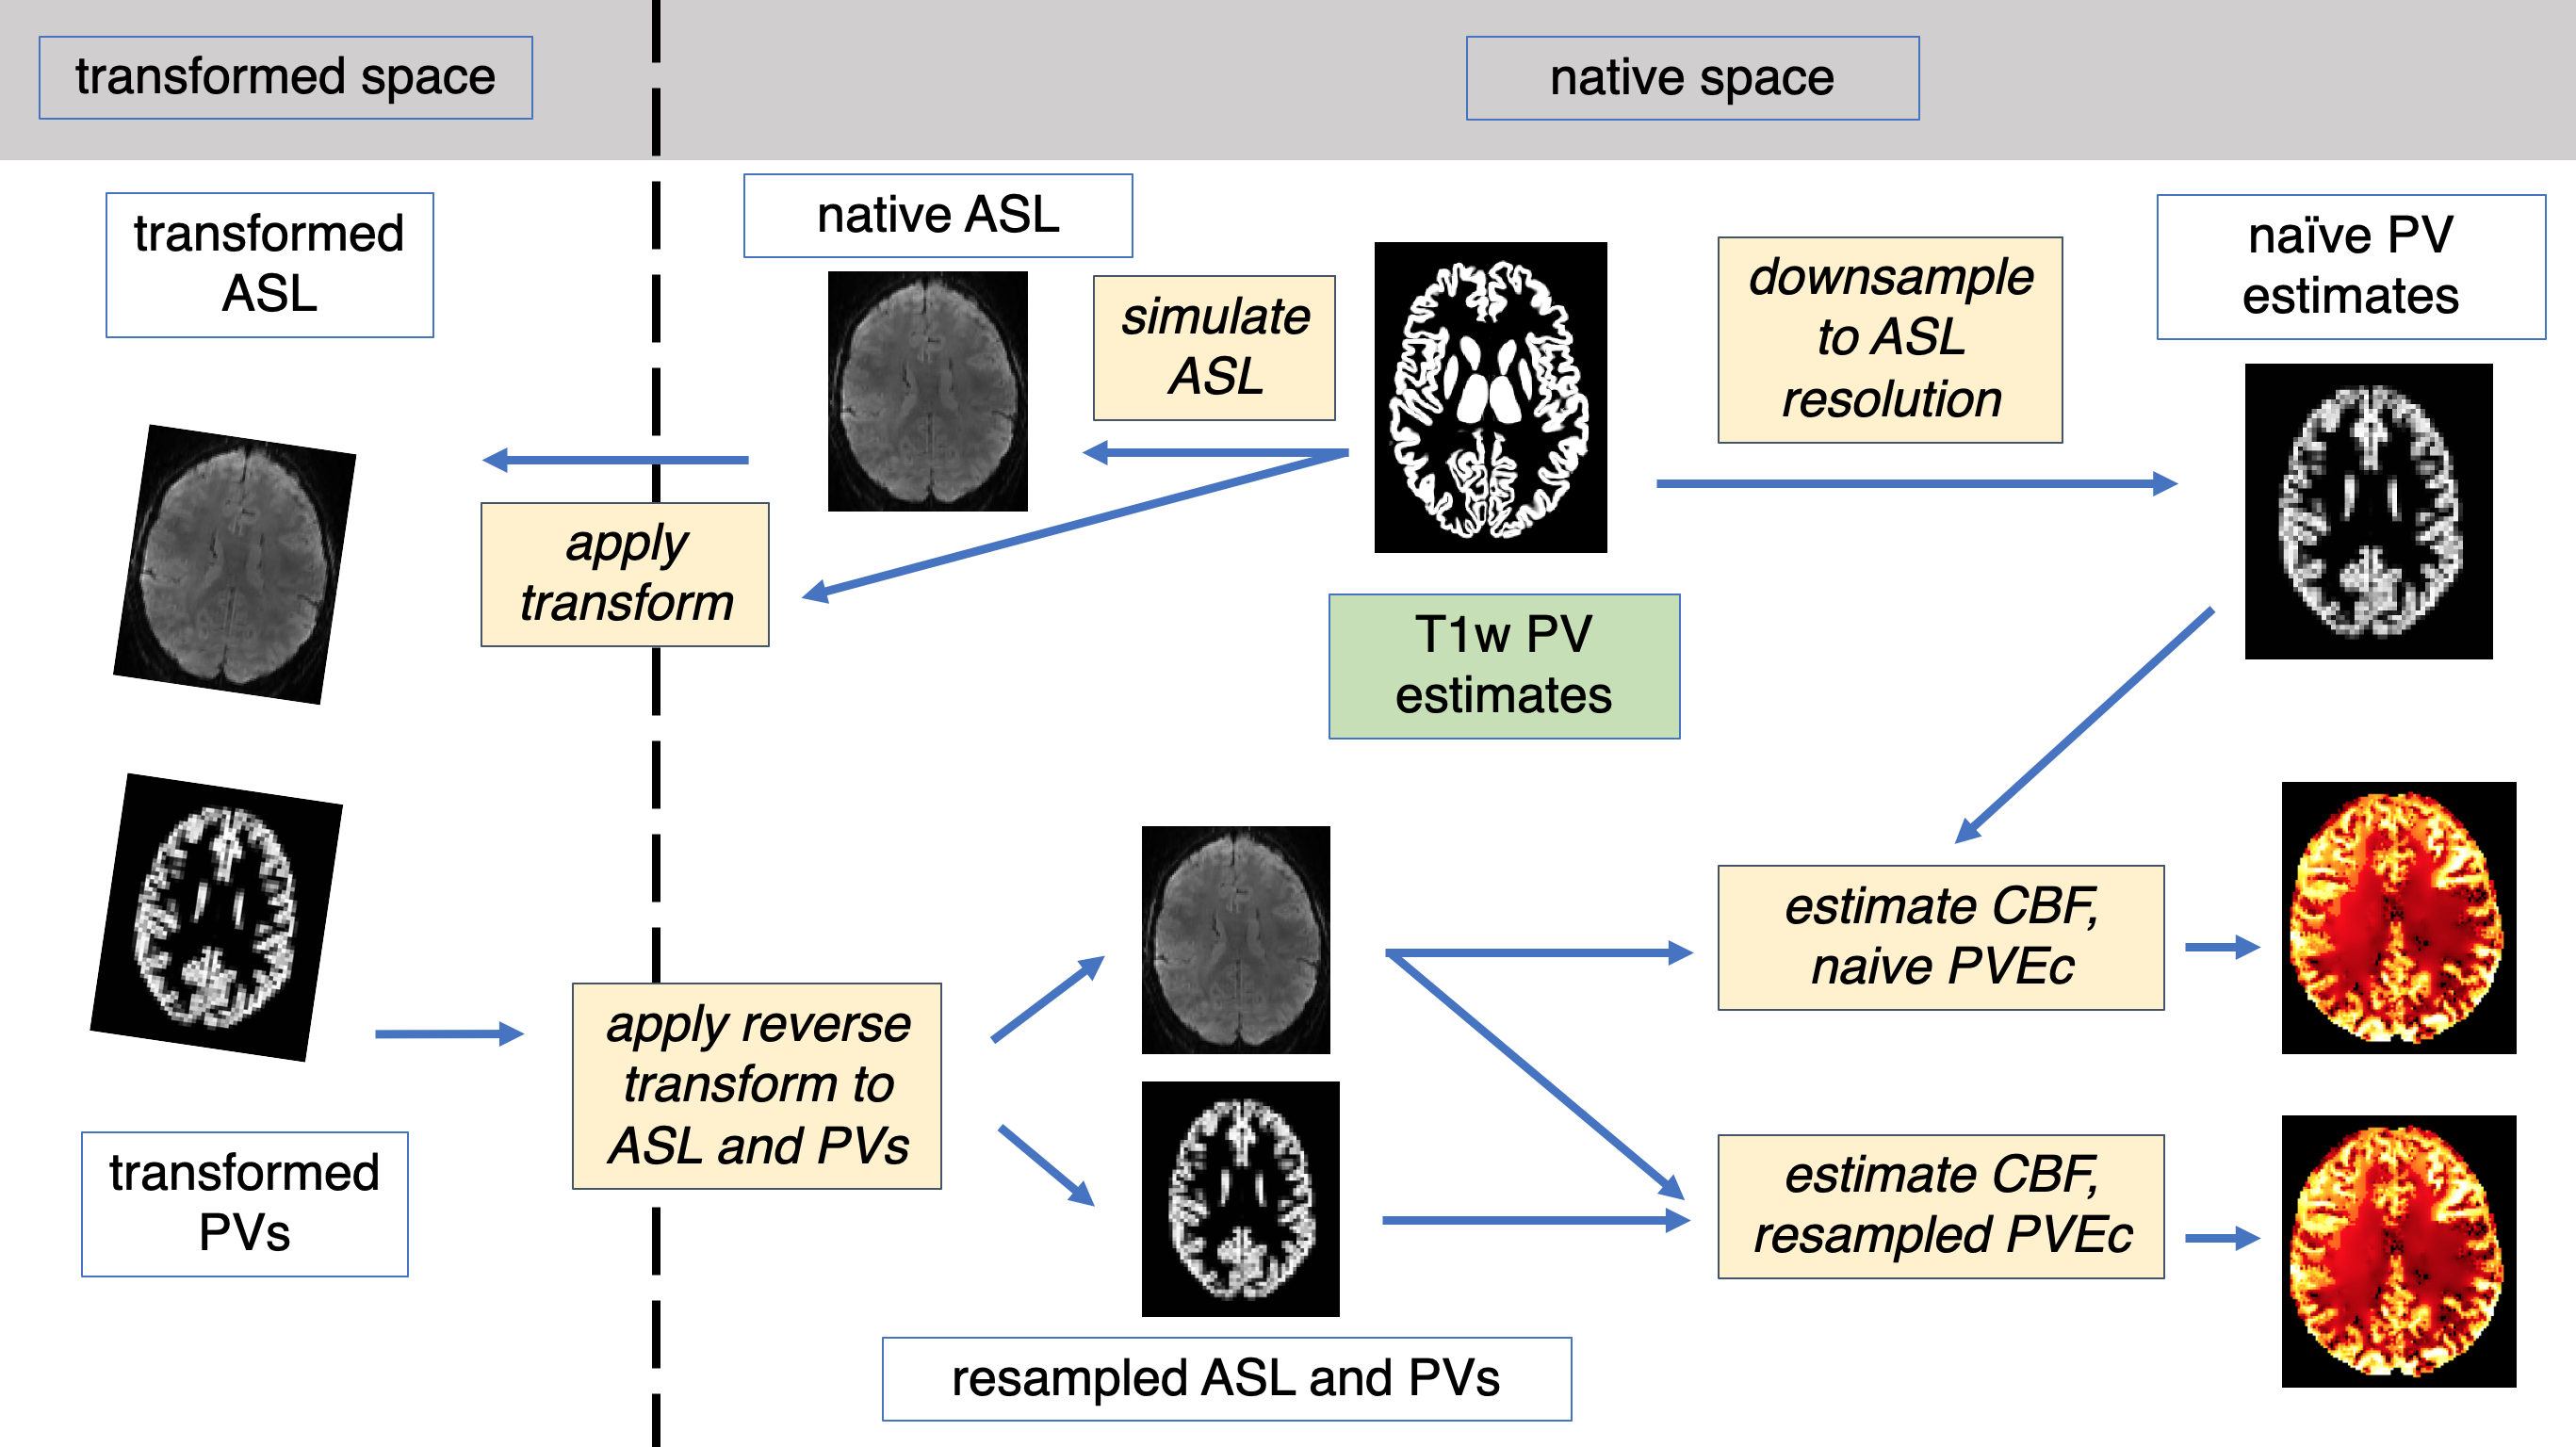
\includegraphics[width = \textwidth]{doublesim_schema.png}
\caption{Schematic of simulation and round-trip transformation for the high SNR simulation data. The point of departure is highlighted in green. ASL data was generated in alignment with the anatomical ground truth PV estimates, and then underwent a round-trip of transformation, alongside the PV estimates. Finally, the transformed ASL data was corrected with both the original PV estimates (naive) and the transformed PV estimates (resampled), and a comparison made with the original data corrected with original PVs (not shown).}
\label{doublesim_schema}
\end{figure}

The extent of PVE within the data was evaluated by drawing histograms of uncorrected voxelwise CBF. The efficacy of PVEc was determined by plotting the distribution of CBF for each tissue after correction; in the ideal case two sharp peaks at 60 and 20 units would be observed for GM and WM respectively. PVEc CBF maps for each tissue were masked to include voxels with at least 5\% of that tissue on the reference (\textit{i.e.}, naive) set of PV estimates. This masking step was necessary because BASIL's PVEc implementation returns tissue CBF estimates for all voxels, including those that do not actually contain the tissue of interest. The strength of the PVE mechanism was evaluated by performing linear regressions of uncorrected CBF against GM PV; theory predicts that CBF should be directly proportional to tissue PV. 

In order to investigate the consequences of transforming repeat data into a common analysis space, simulated ASL repeats were analysed using the schematic given in figure \ref{simrpt_schema}. CBF estimation and PVEc were performed in common space using naive and double-resampled PV estimates. Coefficient of variation (CoV) across the repeats was evaluated in a voxelwise manner by dividing the standard deviation of CBF estimate by the mean. CoV was then averaged within ROIs defined according to GM PV thresholds on the naive set of PV estimates (eight bins of 10\% width, from 20 to 100\% GM PV). This definition of ROI was made purely as a means of establishing spatial correspondence between voxels of the repeated runs, and did \textit{not} genuinely reflect the PVE that are present within each of the runs (which are expected to be different, the very premise of the double-resampled strategy). PVEc CBF maps for each tissue were masked to consider voxels with at least 5\% of the tissue in question. As a final comparator, the individual repeats were also analysed with PVEc in their respective native spaces, and the resultant corrected CBF maps were transformed into the common analysis space. CoV was then calculated in the same manner. This strategy is referred to as `BASIL [or LR] resample after PVEc' and is consistent with the principles of performing all parameter estimation in acquisition-native space and only transforming the outputs.

\begin{figure}[h]
\centering
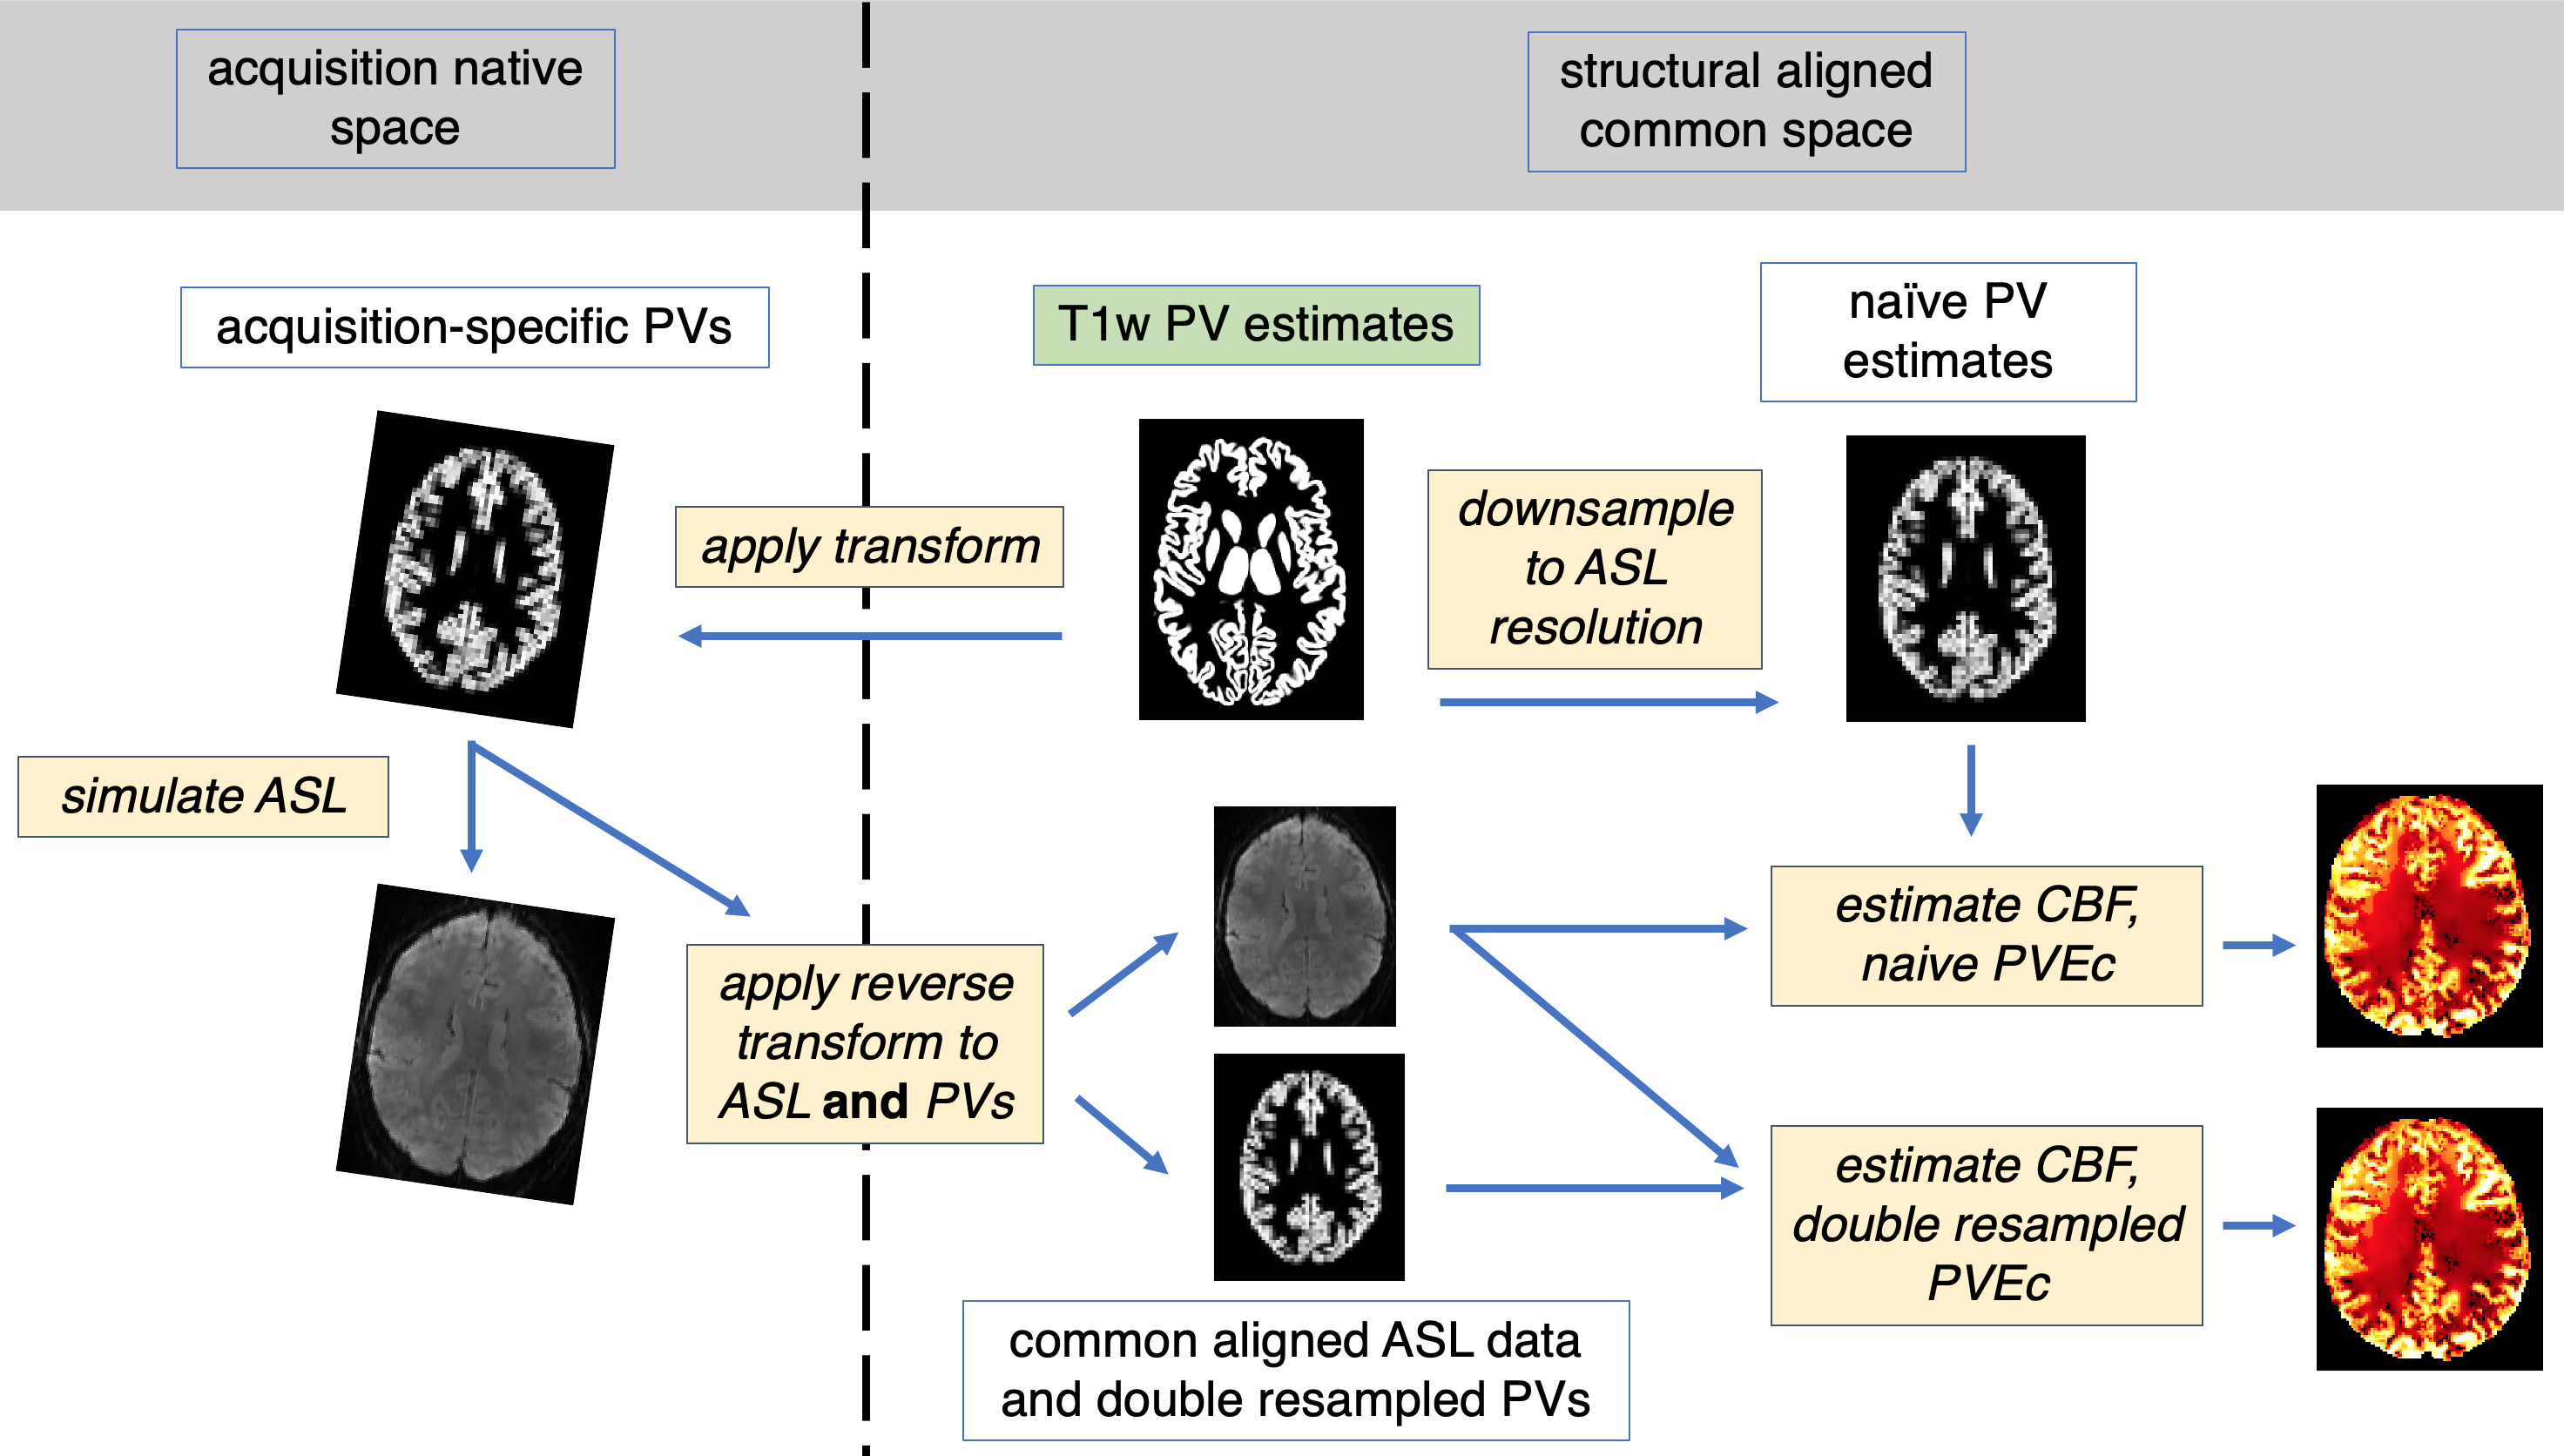
\includegraphics[width = \textwidth]{simrpt_schema.png}
\caption{Schematic of the simulated repeat ASL generation and analysis in common space. The point of departure is highlighted in green. Random transformations were applied to the ground truth PV estimates to yield a unique set of acquisition-specific PVs for each repeat, from which ASL data was then generated. Both the acquisition-specific PVs and ASL data were than transformed back into common space. PVEc of each repeat was performed using both the original PV estimates (naive) and transformed (double-resampled) estimates. As a comparator, PVEc of each repeat was also performed in native space and then the corrected output maps transformed into common space (not shown).}
\label{simrpt_schema}
\end{figure}

\subsection{\textit{In-vivo} data}

The objective of analysis on the \textit{in-vivo} data was to confirm the findings of the simulation experiments. Accordingly, the high SNR ASL data was taken through a round-trip of two resampling operations (using a transformation generated in the same manner as for the simulated repeats). PV estimates were obtained using in the native space of the ASL data the surface-based approach introduced in chapter \ref{tob_pv_chapter}, which then underwent the same set of resampling operations to yield resampled PV estimates. PVEc of the resampled ASL data was then performed using the original and resampled PV estimates. PVEc CBF maps for each tissue were masked to consider voxels with at least 5\% of the tissue in question (as was also the case for the low SNR repeat data). 

The low SNR repeats were analysed in a common analysis space in alignment with the structural image at ASL resolution. CBF estimation and PVEc were performed using both naive and double-resampled PV estimates. The schematic for these strategies was previously set out in figures \ref{rpt_paradox} and \ref{dbl_paradox} respectively. CoV was evaluated in the same manner as for the simulated repeats and ROIs were defined using the same GM PV thresholds on the naive set of PV estimates. As a final comparator, the repeats were also analysed with PVEc in their respective acquisition-native spaces followed by transformation of the output maps into the common space; this strategy is again referred to as `BASIL [or LR] resample after PVEc'. \DIFaddbegin \DIFadd{EPI distortion correction was not performed, which would be expected to lead to areas of mis-alignment between the ASL data and the PV estimates; however due to the global nature of the analysis, the errors arising from this omission should be somewhat mitigated. Overlays of the structural resolution GM PV estimates and native space M0 image, for both the high SNR data and low SNR repeats, are presented in figures \ref{ss_slices} and \ref{02_slices} so that the reader may inspect registration quality and the extent of distortion-induced misalignment. 
}\DIFaddend 

\DIFaddbegin \begin{figure}[H]
\centering
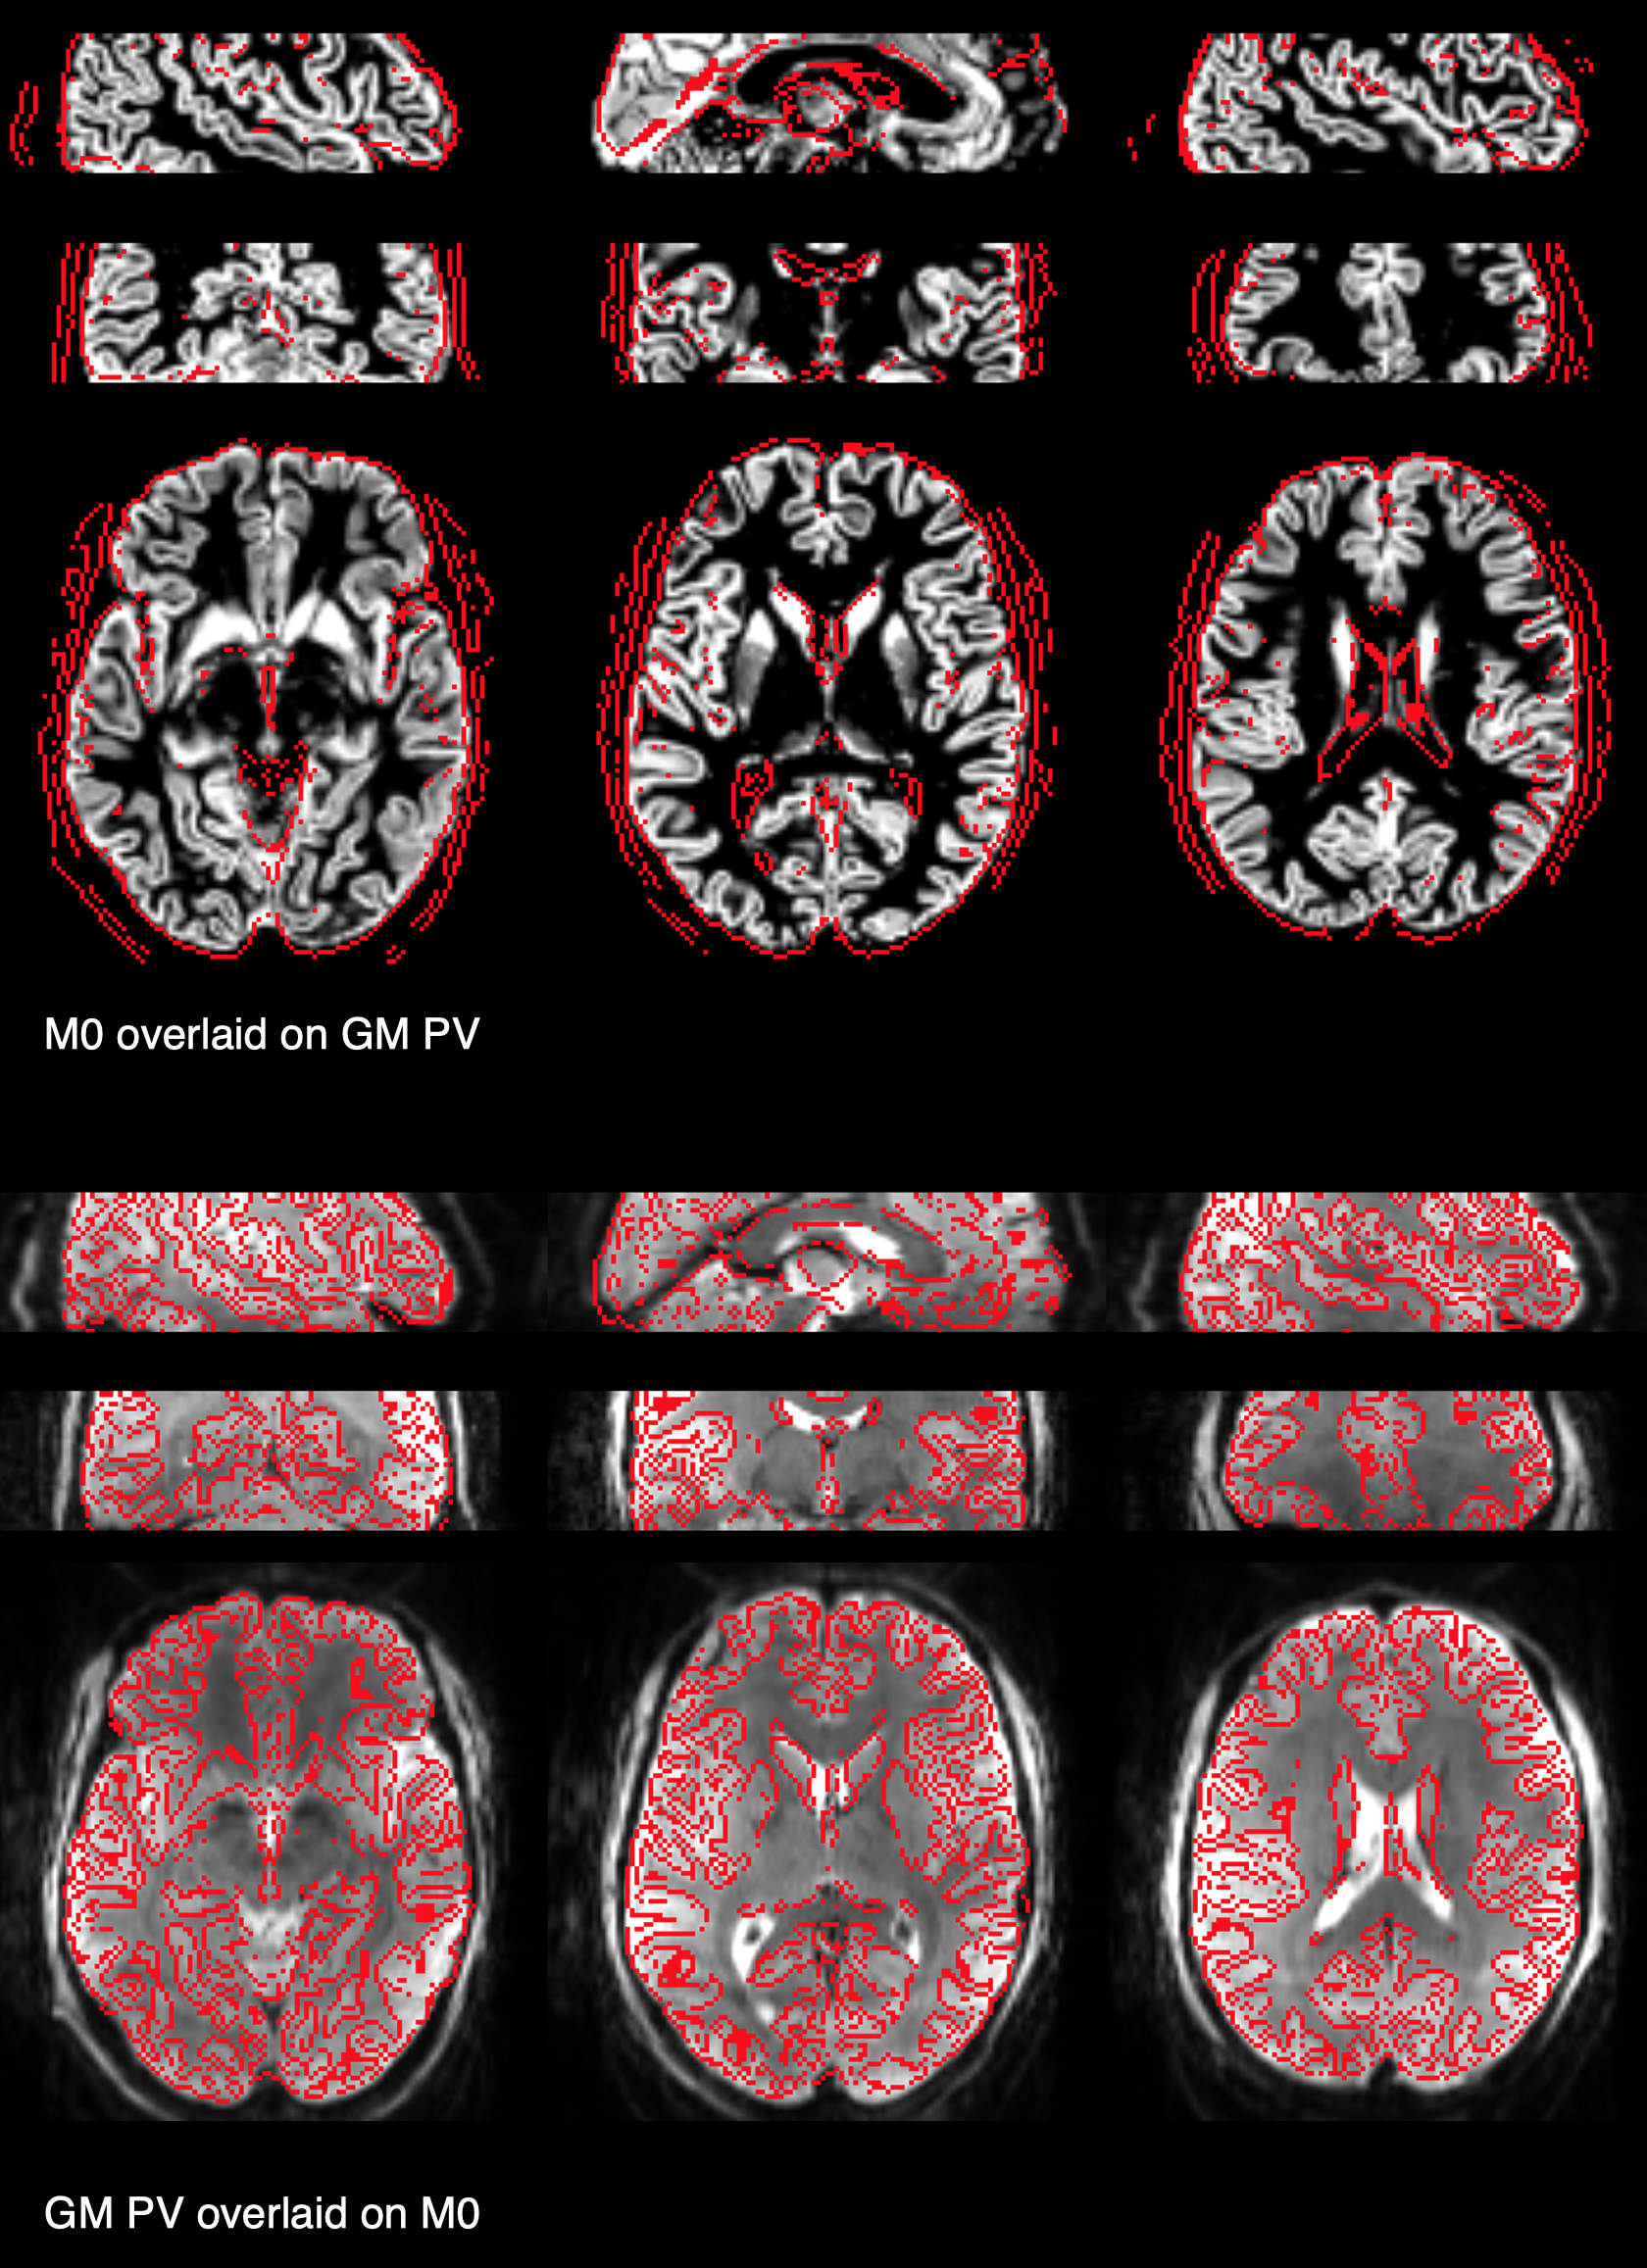
\includegraphics[width = 0.9\textwidth]{slicer/ss_slices.png}
\caption{\DIFaddFL{Alignment between structural (represented by GM PV estimates) and ASL (represented by the M0 image) data, after linear registration but without distortion correction, for the high SNR acquisition. An edge detection filter has been used to better illustrate anatomical boundaries.}}
\label{ss_slices}
\end{figure}

\begin{figure}[H]
\centering
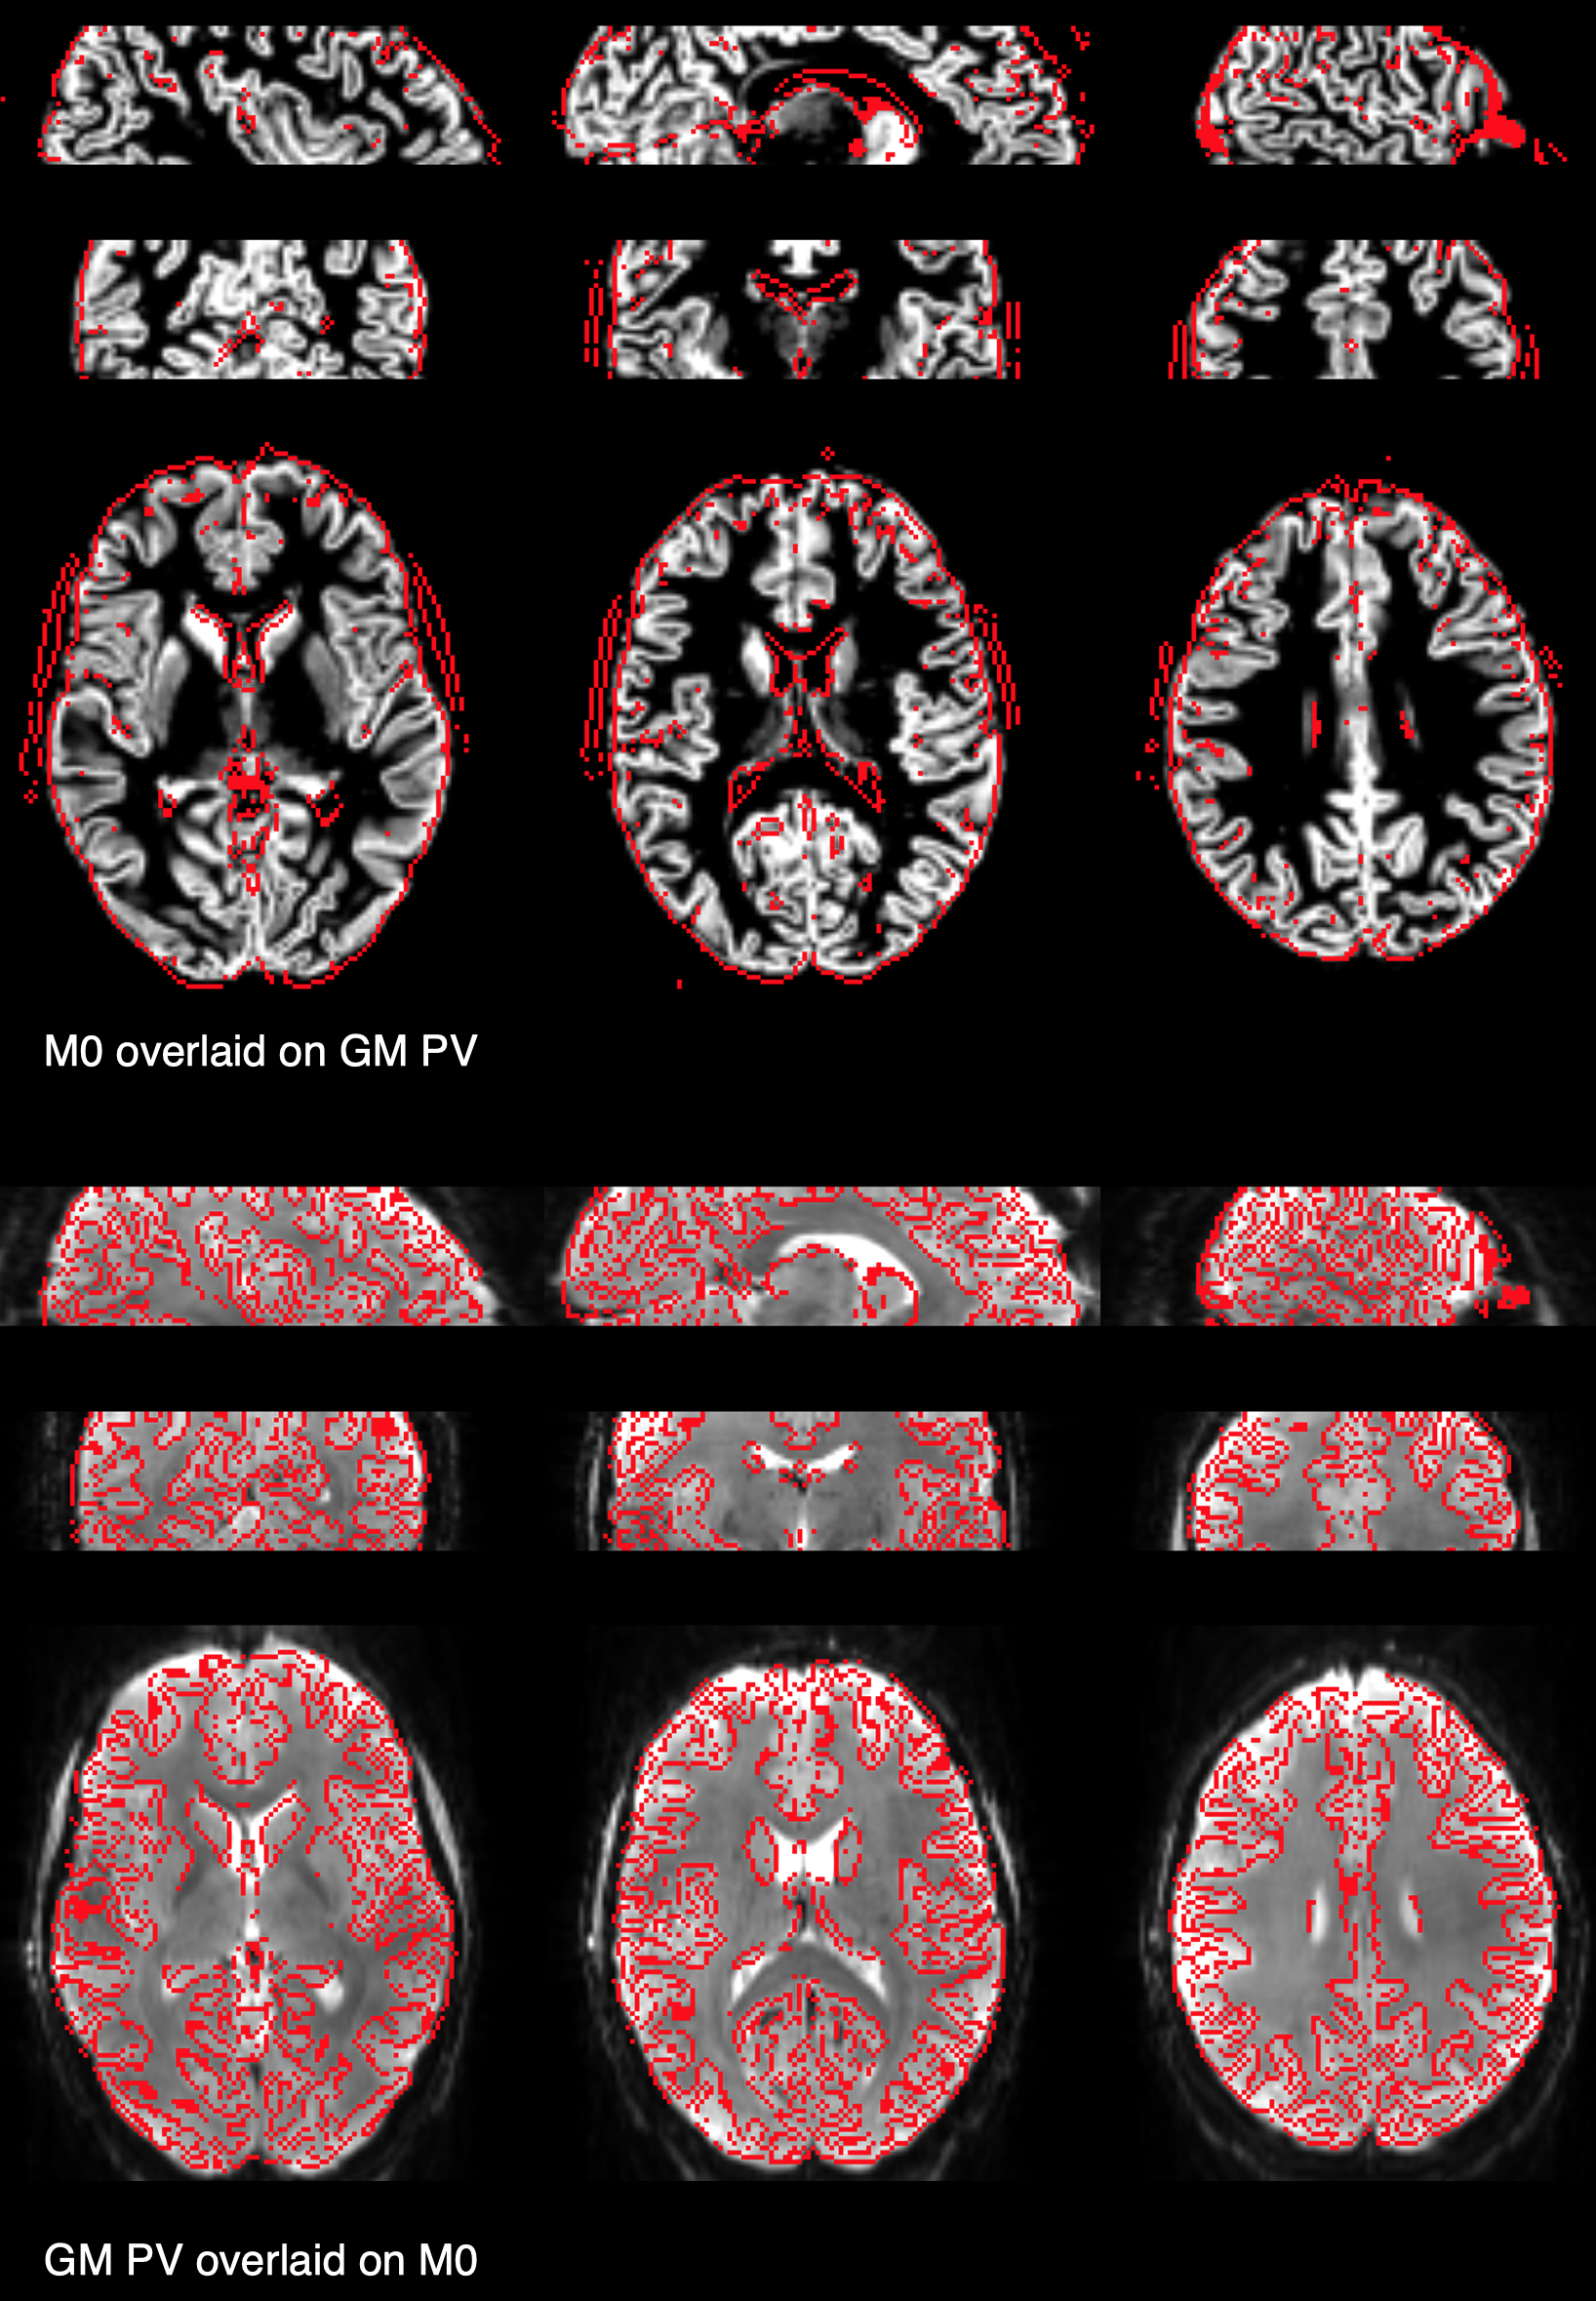
\includegraphics[width = 0.9\textwidth]{slicer/02_slices.png}
\caption{\DIFaddFL{Alignment between structural (represented by GM PV estimates) and ASL (represented by the M0 image) data, after linear registration but without distortion correction, for a single repeat of the low SNR acquisitions. An edge detection filter has been used to better illustrate anatomical boundaries.}}
\label{02_slices}
\end{figure}


\DIFaddend \section{Results}

\subsection{Simulated data}

\subsubsection{High SNR data}

\begin{figure}[H]
\centering
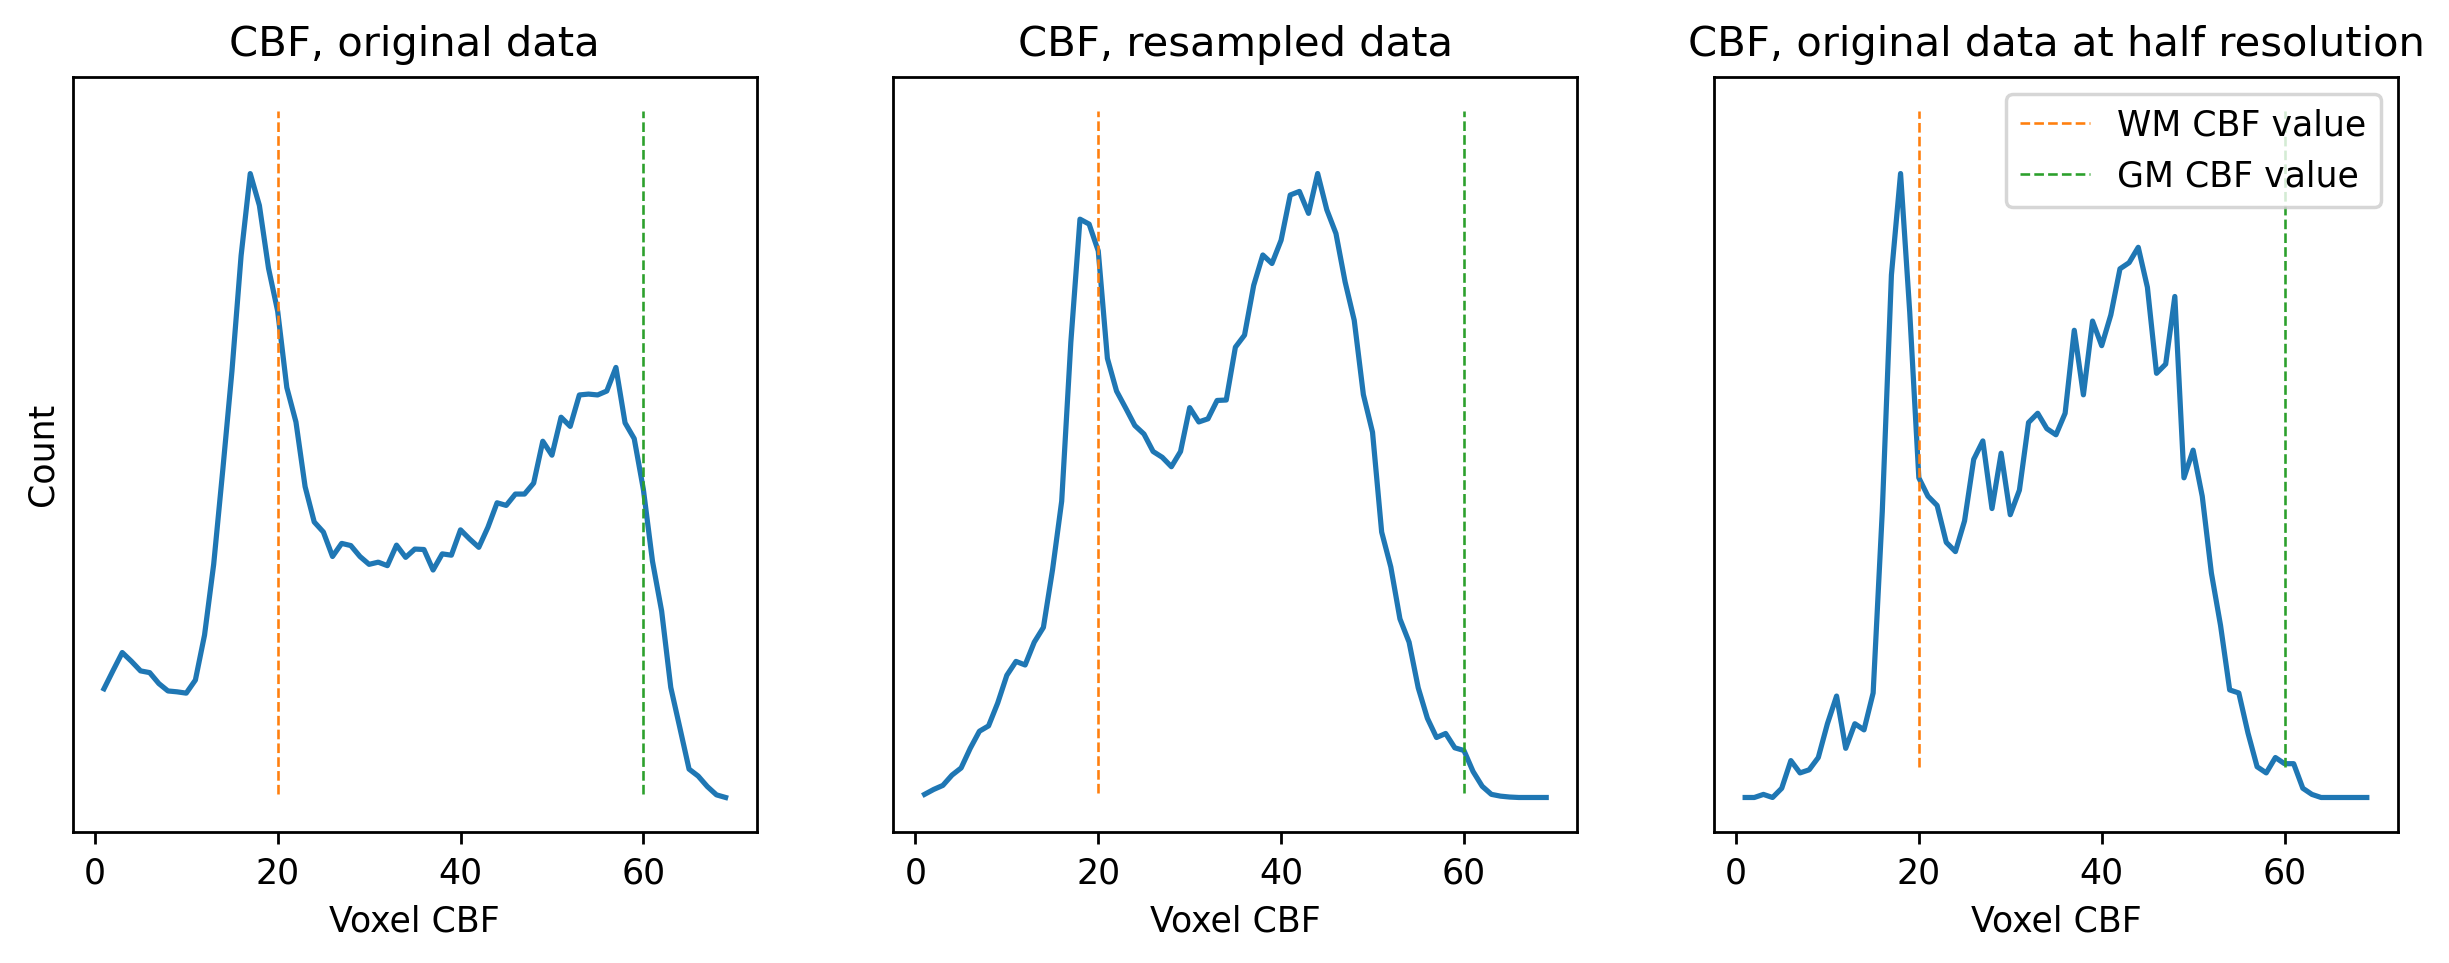
\includegraphics[width = \textwidth]{sim_asl_resamp_hist.png}
\caption{Effect of resampling on PVE within data (all plots show uncorrected CBF). Left: in the base case, CBF from the original data had a bimodal distribution with peaks corresponding to GM and WM CBF values; the extent of PVE is reflected in the large number of voxels that lie in between. Centre: CBF from the resampled data shows convergence of the distribution modes, particularly for the GM peak; this reflects an increase in PVE. Right: CBF from the original data at half the spatial resolution shows many similarities to the resampled case, demonstrating that resampling leads to an increase in PVE that would otherwise be obtained by reducing spatial resolution.}
\label{sim_asl_resamp_hist}
\end{figure}

Figure \ref{sim_asl_resamp_hist} shows histograms of uncorrected CBF estimated from the high SNR simulation data before and after resampling. The distribution of CBF on the original data was bimodal, with peaks corresponding to the ground truth \DIFdelbegin \DIFdel{WM and CBF }\DIFdelend \DIFaddbegin \DIFadd{GM and WM }\DIFaddend values respectively; the presence of PVE was readily observed in the large number of voxels that lie in between these modes. After a round-trip of resampling there was a clear convergence between the modes of the distribution (in particular, the peak corresponding to GM shifted from around 60 to 40 units), indicating an increase in PVE. This change was consistent with what would be obtained if one had estimated CBF from the original data at half the spatial resolution (which is shown in the final plot). 

\begin{figure}[H]
\centering
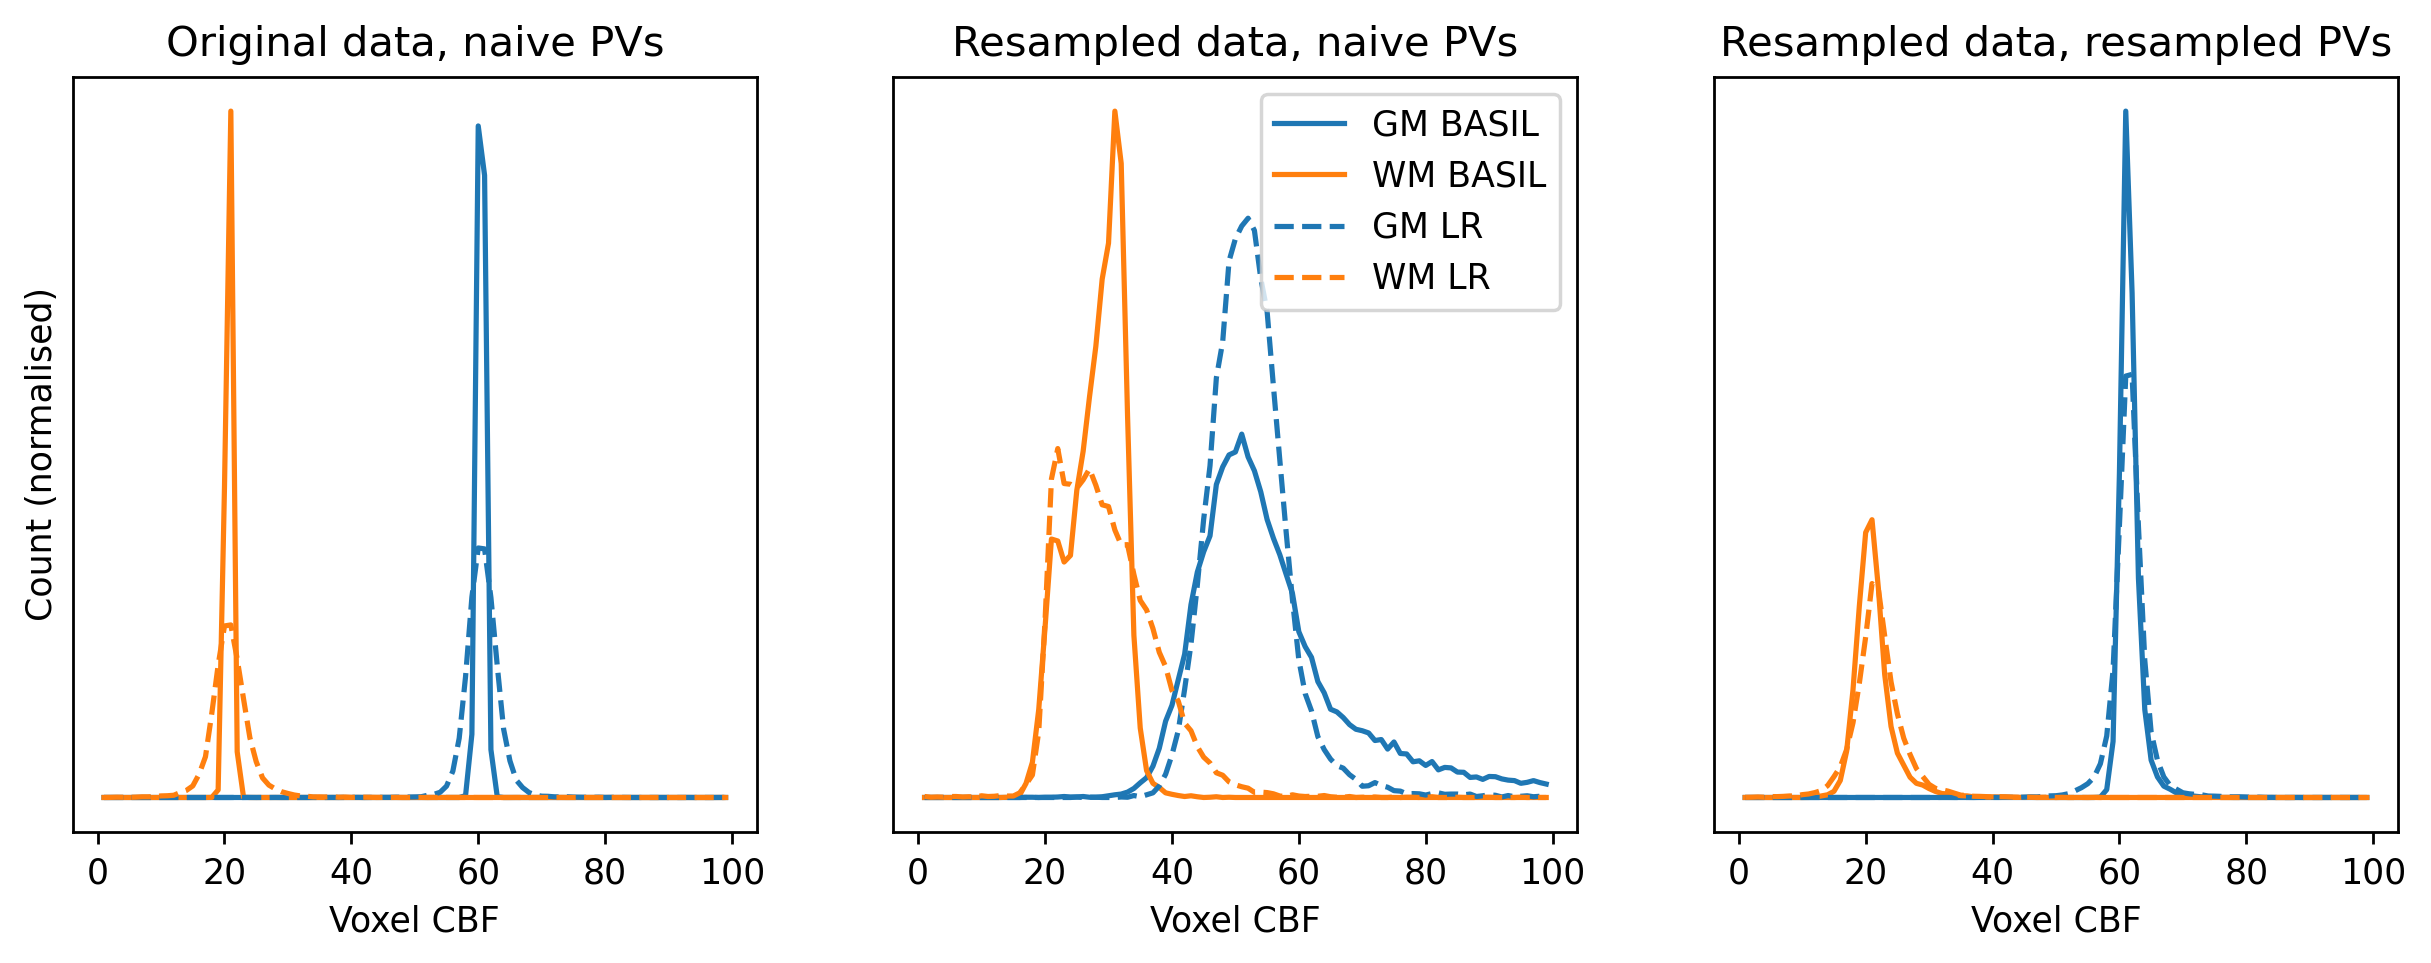
\includegraphics[width = \textwidth]{sim_asl_resamp_pvec.png}
\caption{Outcomes of PVEc on data before and after resampling. Left: for the base case of no resampling, PVEc of either form was able to recover ground truth CBF values for both tissues. Centre: after resampling, PVEc with the naive PV estimates led to poor recovery of ground truth. BASIL particularly struggled for GM whereas the LR method struggled for WM. Right: PVEc of the resampled data with the resampled PV estimates led to excellent recovery of ground truth, a result that was almost identical to the base case without resampling.}
\label{sim_asl_resamp_pvec}
\end{figure}

Figure \ref{sim_asl_resamp_pvec} shows the outcomes of PVEc on the high SNR simulation data before and after resampling. PVEc of either form on the original data was able to recover the ground truth values for GM and WM CBF. Following a round-trip of resampling, PVEc with the naive PV estimates led to poor recovery of ground truth for either method. BASIL displayed positive skew in GM but was more symmetric in WM, whereas the reverse was true for the LR method. Finally, PVEc with the double-resampled PV estimates showed a substantial improvement over the naive approach; the results were essentially identical to the base case established without resampling. 

\begin{figure}[H]
\centering
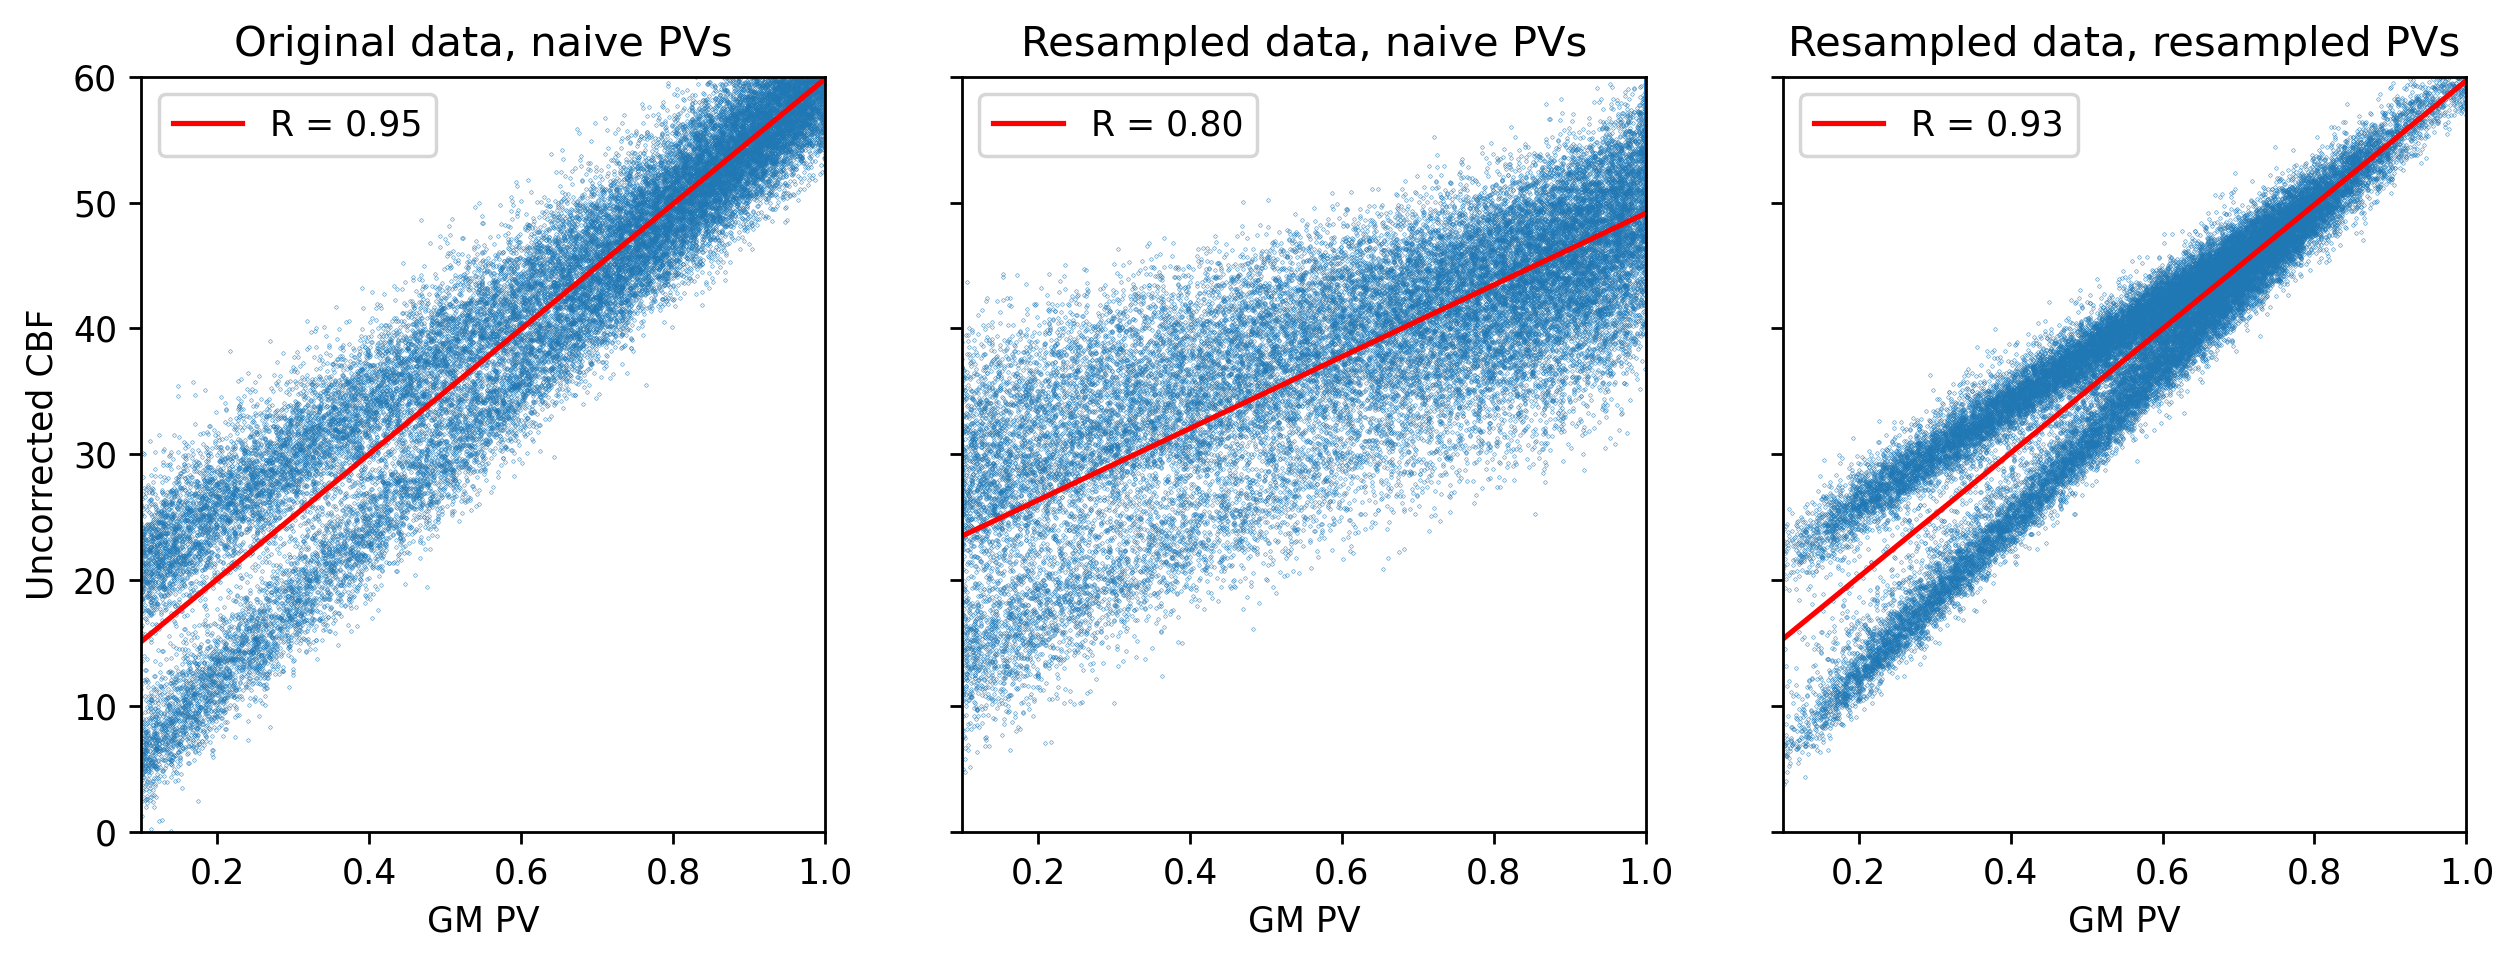
\includegraphics[width = \textwidth]{sim_asl_resamp_scatter.png}
\caption{Scatter plots of uncorrected CBF against GM PV before and after resampling. Left: the base case of no resampling showed a very strong correlation coefficient ($R$ = 0.95). Centre: a scatter of CBF from resampled data against naive GM PV showed a substantial decrease in $R$ to \DIFdelbeginFL \DIFdelFL{0.79}\DIFdelendFL \DIFaddbeginFL \DIFaddFL{0.80}\DIFaddendFL , indicating that the naive PVs did not correlate with the PVE of the data as well. Right: scatter against the resampled GM PV, which showed an increase in $R$ to \DIFdelbeginFL \DIFdelFL{0.89}\DIFdelendFL \DIFaddbeginFL \DIFaddFL{0.93}\DIFaddendFL . This indicated that the resampled PVs better reflect the PVE that were actually embedded in the data after resampling.}
\label{sim_asl_resamp_scatter}
\end{figure}

Figure \ref{sim_asl_resamp_scatter} shows voxelwise scatter plots of GM PV against uncorrected CBF derived from the high SNR simulation data before and after resampling. Linear regressions were performed in each case. Prior to resampling, there was an extremely strong relationship between CBF and GM PV with correlation coefficient ($R$ value) of 0.95. This reflects the nature in which the data was generated, namely in direct proportion to the PVs present in each voxel with no underlying parameter variation. The bimodal distribution of CBF could clearly be observed in the two separate lines that the voxels clustered around. Following resampling of the ASL data, a scatter of CBF against naive GM PV showed a substantial decrease in $R$ to \DIFdelbegin \DIFdel{0.79}\DIFdelend \DIFaddbegin \DIFadd{0.80}\DIFaddend . This decrease indicated that the naive PVs no longer explained the variance observed in the resampled data to the same extent as before. Finally, a scatter against the double-resampled GM PV showed an improvement in $R$ to \DIFdelbegin \DIFdel{0.89}\DIFdelend \DIFaddbegin \DIFadd{0.93}\DIFaddend , 
largely recovering the original value in the base case. The increase in $R$ value indicated that the double-resampled PVs better matched the extra PVE that were embedded within the data following resampling. 

\begin{figure}[H]
\centering
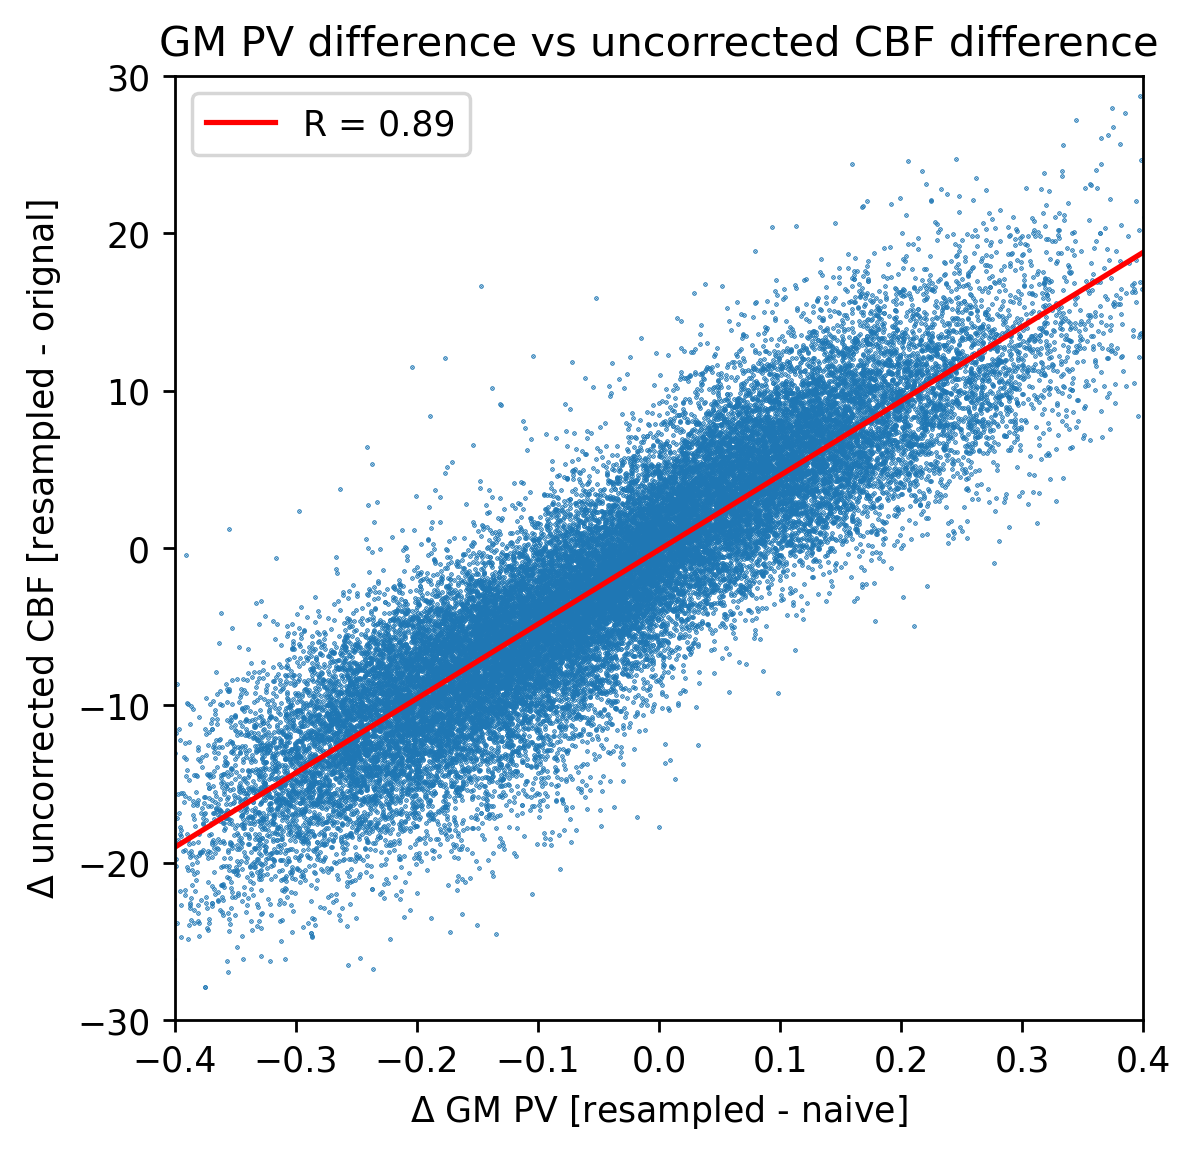
\includegraphics[width = 0.6\textwidth]{sim_asl_deltapv_deltacbf.png}
\caption{Scatter plot of change in GM PV against change in uncorrected CBF. Change in either quantity was defined as the resampled variable minus the original. The high correlation coefficient demonstrated that the change in CBF arising due to resampling of the ASL data could almost entirely be explained by a change in the corresponding voxel PV.}
\label{sim_asl_deltapv_deltacbf}
\end{figure}

Figure \ref{sim_asl_deltapv_deltacbf} shows a scatter plot of change in GM PV against change in uncorrected CBF before and after resampling. For both quantities, the change was defined as the resampled variable minus the original (for example, CBF of resampled data minus CBF of original). A high correlation coefficient was observed ($R$ = \DIFdelbegin \DIFdel{0.89}\DIFdelend \DIFaddbegin \DIFadd{0.95}\DIFaddend ), which implied that the change in uncorrected CBF was largely explained by a corresponding change in GM PV. This shows that applying the same resampling to the PV estimates does convey meaningful information about the extra PVE that are introduced into the ASL data. For voxels that lost GM as a result of resampling, uncorrected CBF was reduced, which was in agreement with the theoretical foundations of PVE. 

\subsubsection{Low SNR repeats}

\begin{figure}[H]
\centering
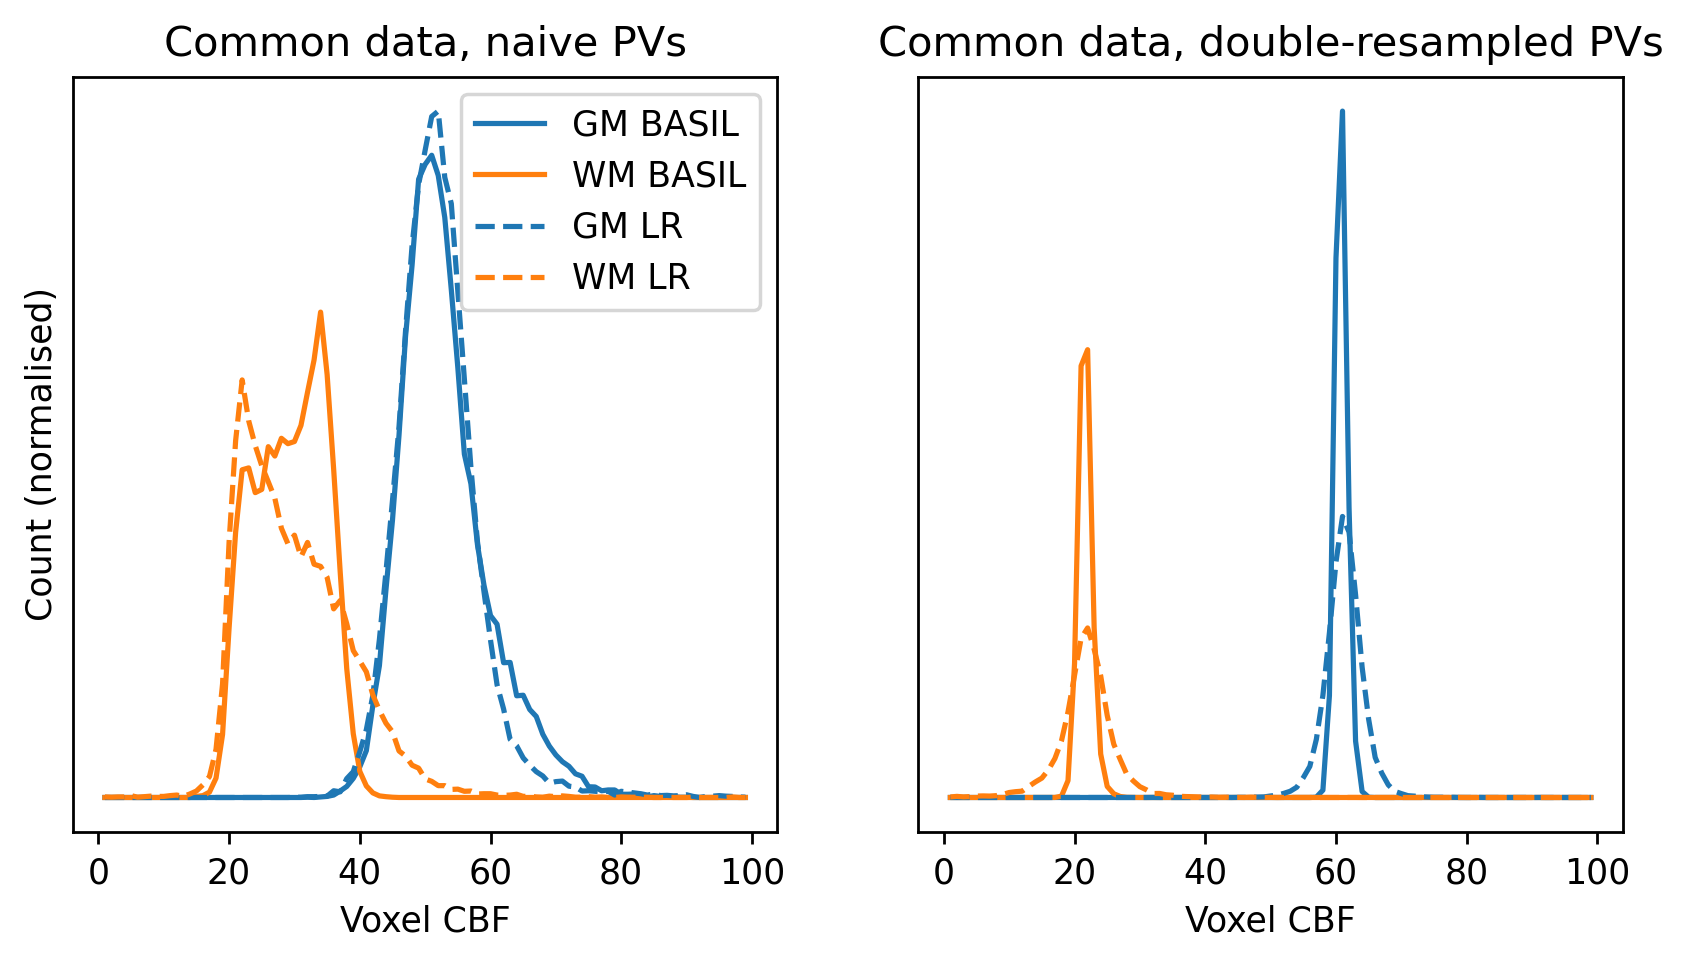
\includegraphics[width = 0.75\textwidth]{sim_rpts_resamp_pvec.png}
\caption{Histograms of PVEc CBF for simulated repeat data in common analysis space. The mean distribution across repeats is shown. Left: PVEc with the naive PV estimates led to a poor recovery of ground truth, whereas (Right:) PVEc with the double-resampled PV estimates performed much better. Both of these findings were in agreement with the results of the high SNR simulation shown in figure \ref{sim_asl_resamp_pvec}.}
\label{sim_rpts_resamp_pvec}
\end{figure}

Figure \ref{sim_rpts_resamp_pvec} shows histograms of PVEc CBF on the simulated repeat data in common analysis space. In both plots the mean distribution across repeats is shown. PVEc of the common-aligned data with naive PVs showed poor recovery of the ground truth, whereas PVEc with double-resampled PVs showed a significant improvement in recovery of the ground truth distributions. Both of these results were in agreement with those observed on the high SNR simulation (figure \ref{sim_asl_resamp_pvec}). This result implied that accurately conveying the different PVE embedded within repeat data is key to successful PVEc in a non-native analysis space.  

\begin{figure}[H]
\centering
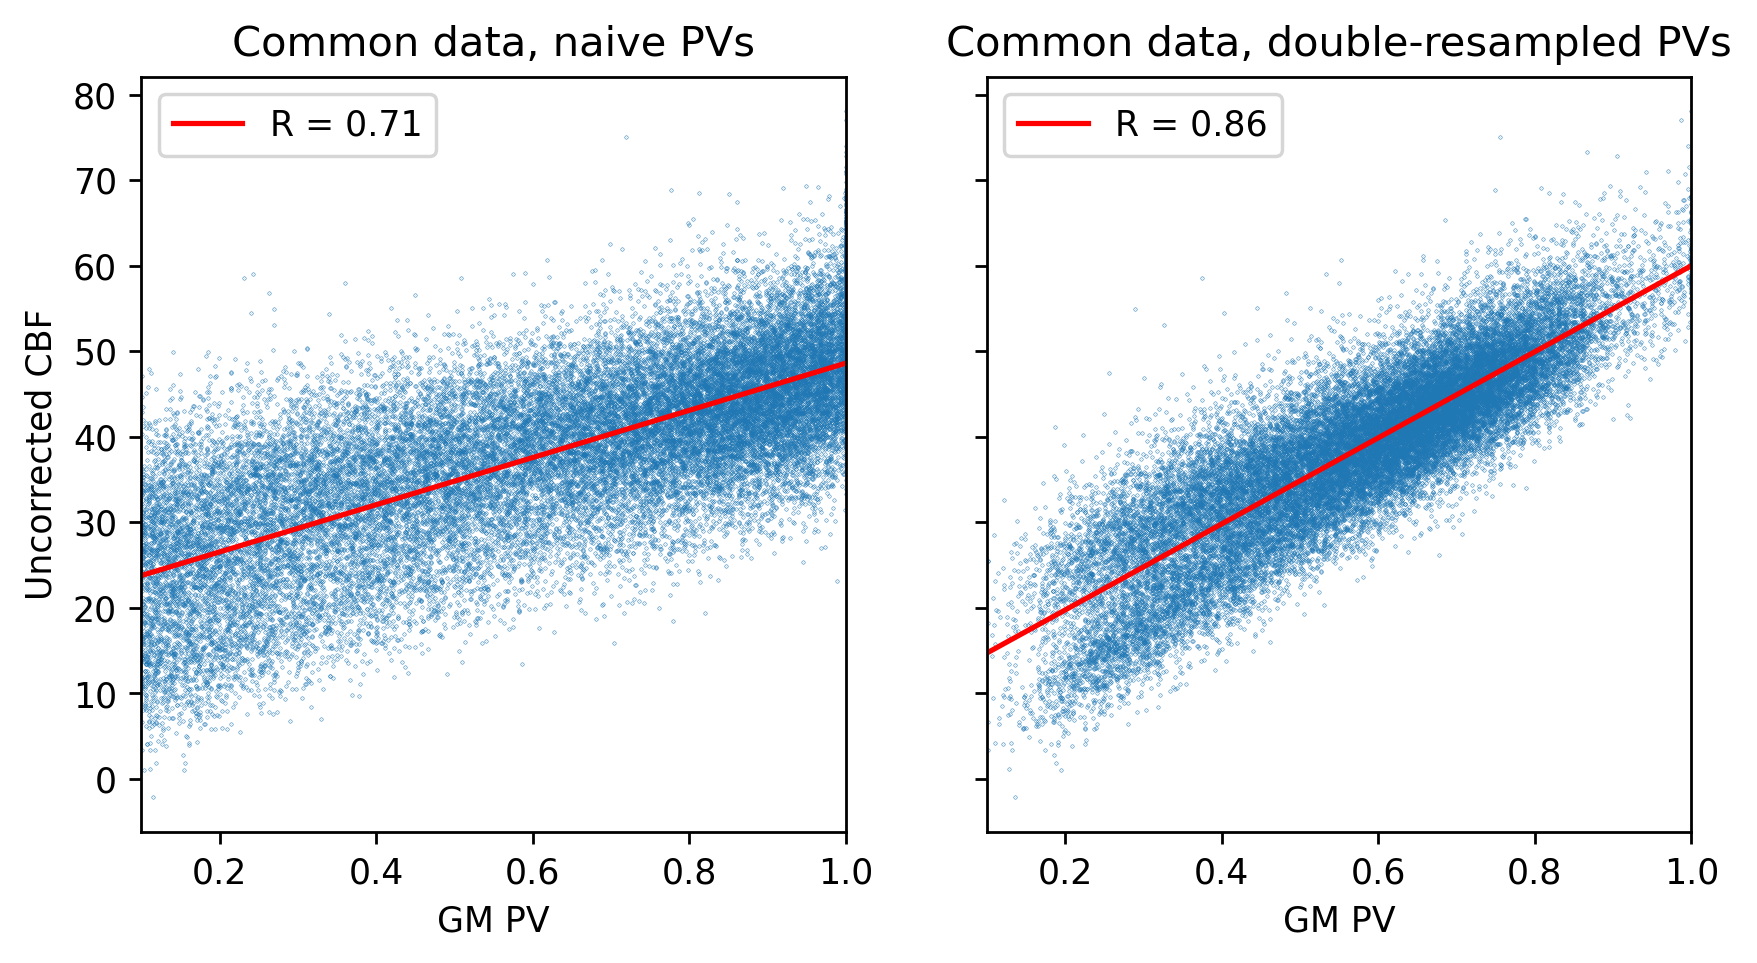
\includegraphics[width = 0.75\textwidth]{sim_rpts_resamp_scatter.png}
\caption{Scatter plots and linear regressions of uncorrected CBF for a single repeat of simulated data in common space. Left: a scatter against naive GM PV; Right: a scatter against double-resampled GM PV. The correlation coefficient for the double-resampled PVs was stronger, indicating that they better explained the variability seen in the data.}
\label{sim_rpts_resamp_scatter}
\end{figure}

Figure \ref{sim_rpts_resamp_scatter} shows scatter plots and linear regressions of uncorrected CBF estimated from the repeat data in common analysis space. The regressions were performed against the naive GM PV estimates and the double-resampled GM PV estimates (a single repeat's worth of data was used). Again mirroring the results from the high SNR simulation case (figure \ref{sim_asl_resamp_scatter}), the correlation coefficient for the double-resampled PVs was greater than for the naive PVs ($R$ = \DIFdelbegin \DIFdel{0.81 }\DIFdelend \DIFaddbegin \DIFadd{0.86 }\DIFaddend vs. 0.71). This showed that the double-resampled PVs better matched the PVE that were embedded within the ASL data after resampling into the common space. Both correlation coefficients were smaller than the high SNR case, which was presumed to be due to the presence of increased noise in the repeat data. 


\begin{figure}[H]
\centering
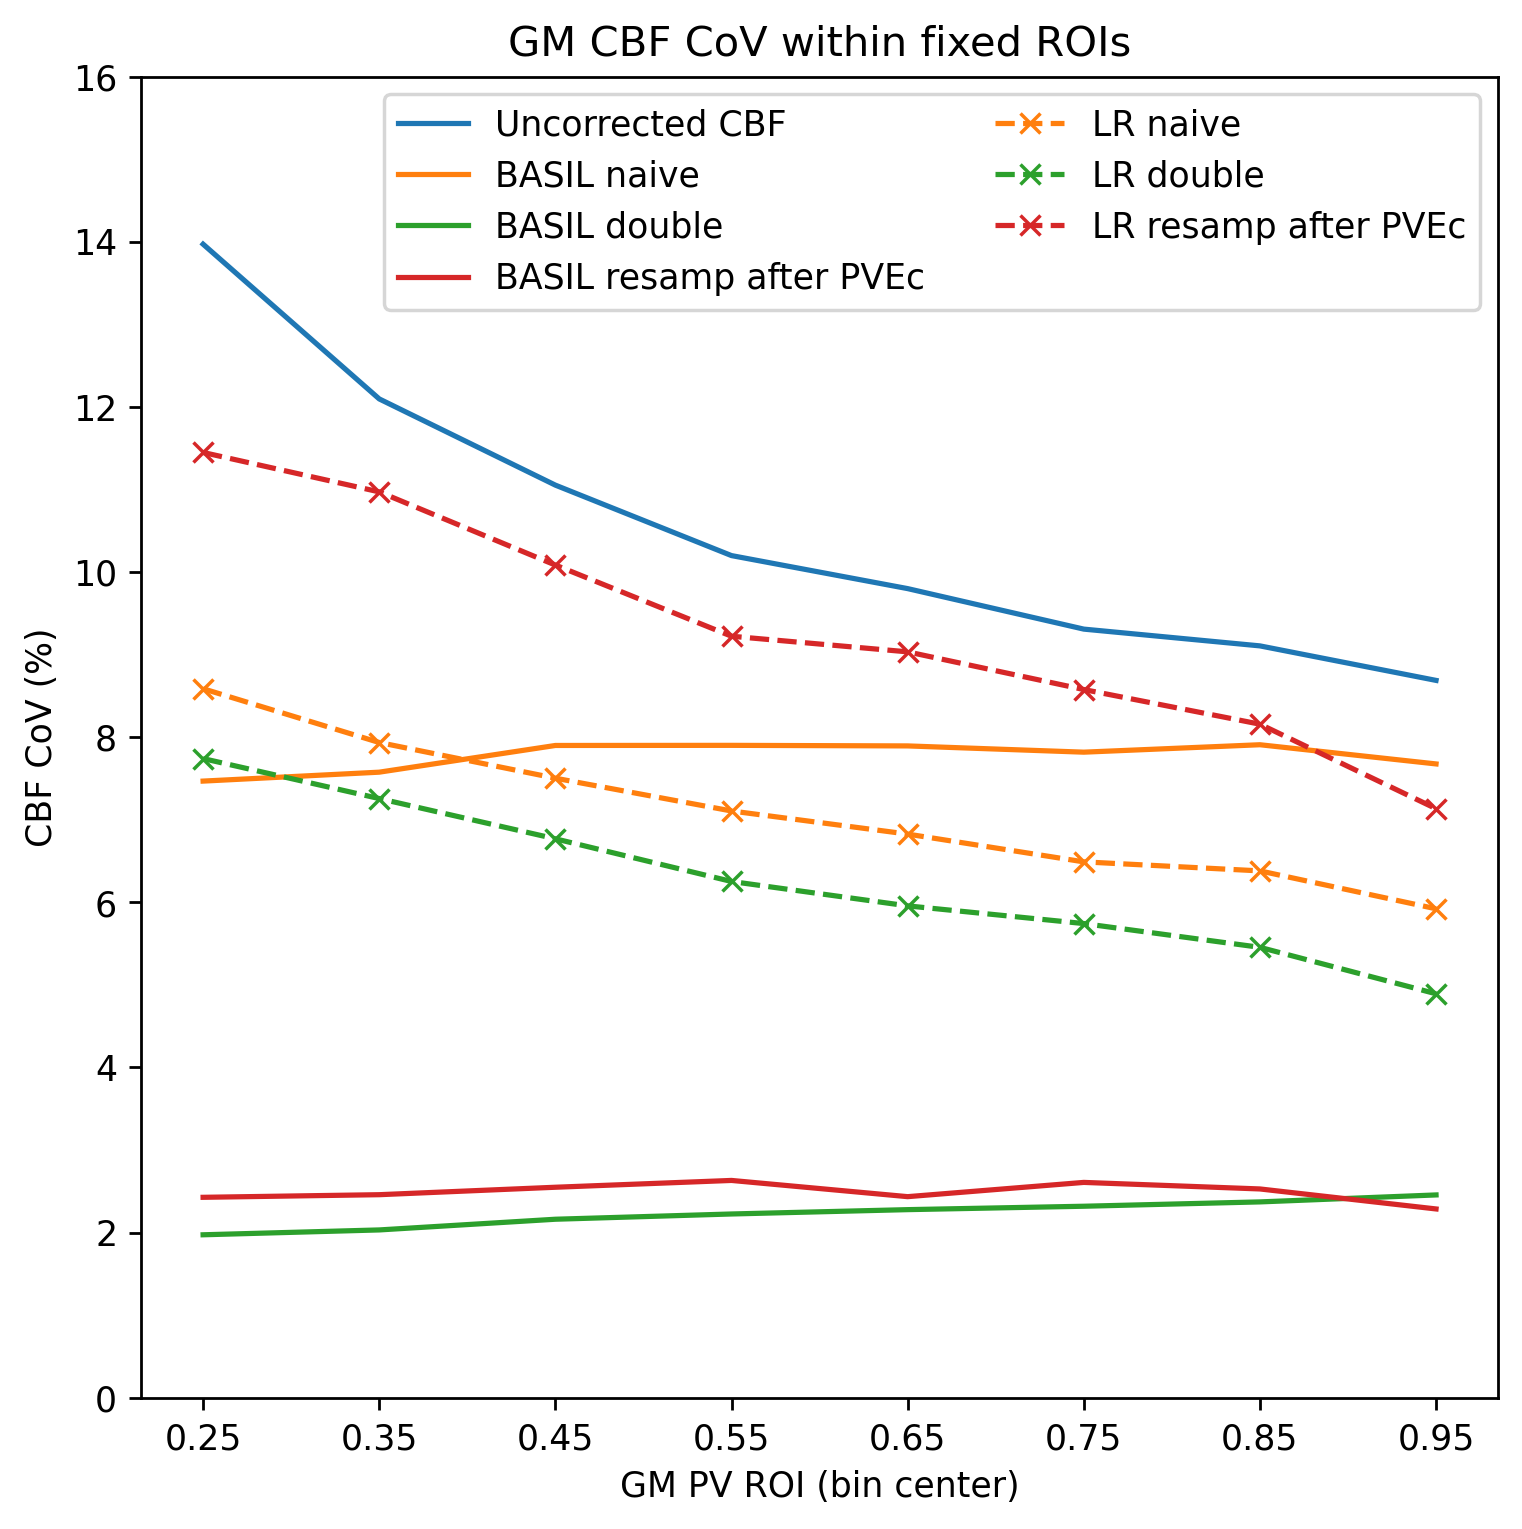
\includegraphics[width = 0.6\textwidth]{sim_lowsnr_cov.png}
\caption{CoV of CBF measurement in common analysis space across simulated repeats. The blue trace represents the baseline case of no PVEc. For both BASIL and the LR method, PVEc with double-resampled PV estimates (green) resulted in smaller CoV than for naive PV estimates (orange).}
\label{sim_lowsnr_cov}
\end{figure}

Figure \ref{sim_lowsnr_cov} shows the coefficient of variation across all simulated repeats for CBF measurement within voxel ROIs. The baseline case of uncorrected CBF was established: this was expected to lead to a higher CoV, due to the differing levels of PVE within the individual repeats feeding through to their resultant CBF estimates. CoV of uncorrected CBF decreased for ROIs defined with a higher proportion of GM PV, which was in agreement with theory (in the limit, voxels that are pure GM should have identical CBF due to the assumption of constant CBF underpinning these simulations). For both BASIL and the LR method, PVEc with double-resampled PV estimates resulted in lower CoV than with the naive PV estimates.
\DIFdelbegin \DIFdel{BASIL's double-resampled PVEc led to the lowest CoV for all ROIs of all methods, whereas BASIL's naive PVEc actually returned higher CoV than the baseline case of uncorrected CBF. 
}\DIFdelend 

\subsection{\textit{In-vivo} data}

\subsubsection{High SNR data}

\begin{figure}[H]
\centering
\DIFaddbeginFL 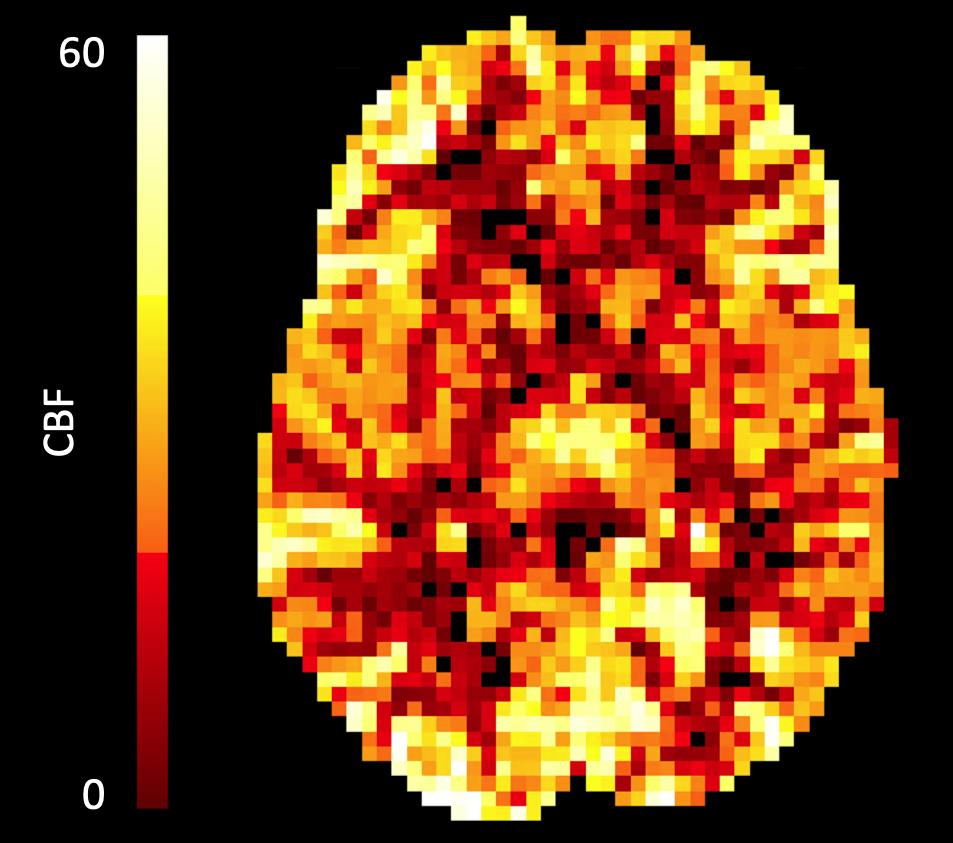
\includegraphics[width = 0.75\textwidth]{ss_asl.png}
\caption{\DIFaddFL{Axial slice of uncorrected CBF estimates derived from the high data in native space (without resampling).}}
\label{ss_asl}
\end{figure}

\DIFadd{Figure \ref{ss_asl} shows an axial slice from the uncorrected CBF estimates derived from the high SNR data in native space (prior to resampling). This provides the basis for the distributions drawn in figure \ref{real_resamp_hist}. 
}

\begin{figure}[H]
\centering
\DIFaddendFL 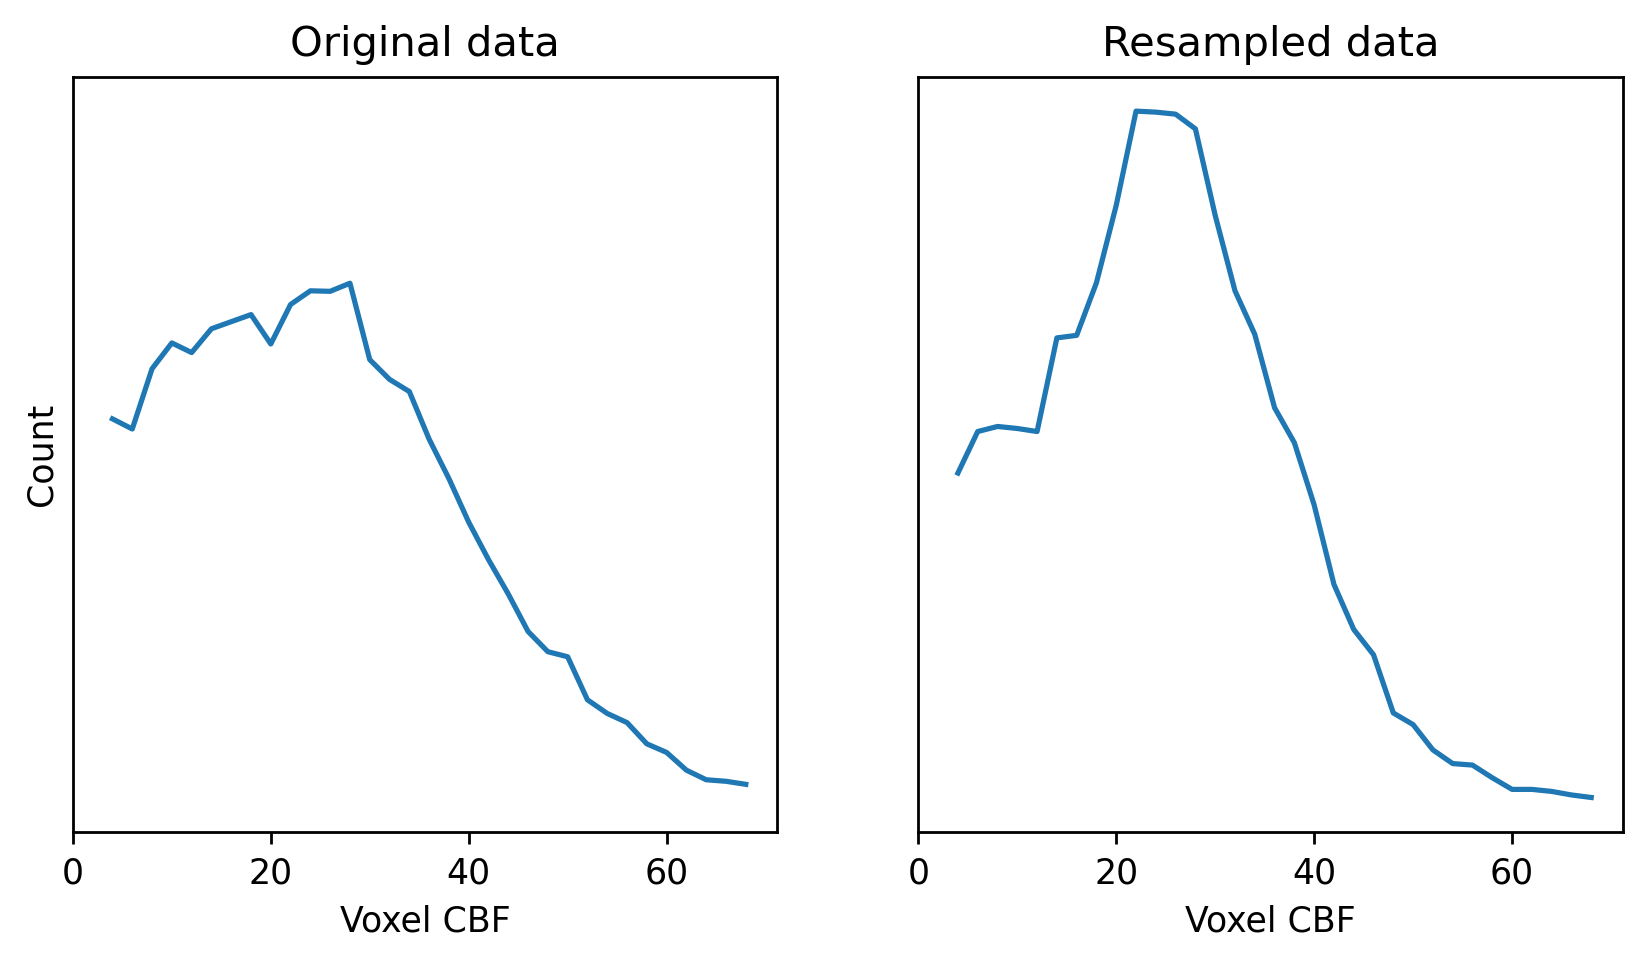
\includegraphics[width = 0.75\textwidth]{real_resamp_hist.png}
\caption{Distributions of uncorrected CBF from the high SNR \textit{in-vivo} data before (left) and after (right) resampling. The effect of resampling was to shift \DIFaddbeginFL \DIFaddFL{more voxels into }\DIFaddendFL the \DIFdelbeginFL \DIFdelFL{peak }\DIFdelendFL \DIFaddbeginFL \DIFaddFL{centre }\DIFaddendFL of the distribution\DIFdelbeginFL \DIFdelFL{from around 0 units to 10}\DIFdelendFL , \DIFdelbeginFL \DIFdelFL{making it more Gaussian and }\DIFdelendFL consistent with \DIFdelbeginFL \DIFdelFL{increasing PVE within }\DIFdelendFL \DIFaddbeginFL \DIFaddFL{increased mixing of CBF between voxels. There was a corresponding reduction in }\DIFaddendFL the \DIFdelbeginFL \DIFdelFL{data}\DIFdelendFL \DIFaddbeginFL \DIFaddFL{number of voxels with CBF $>$ 40\cbf{}}\DIFaddendFL .}
\label{real_resamp_hist}
\end{figure}

Figure \ref{real_resamp_hist} shows \DIFaddbegin \DIFadd{distributions of }\DIFaddend uncorrected CBF estimated from the high SNR \textit{in-vivo} data, before and after a round-trip of resampling. The distribution was not bimodal (as was the case for the high SNR simulation case in figure \ref{sim_asl_resamp_hist})\DIFdelbegin \DIFdel{; instead it was monotonic decreasing for increasing CBF}\DIFdelend \DIFaddbegin \DIFadd{, but nevertheless the effect of resampling could be observed}\DIFaddend . After a round-trip of resampling, the \DIFdelbegin \DIFdel{the peak of the distribution shifted substantially (from around 0 units to 10 units) . Though the exact nature of the distribution was somewhat different to the idealised case established in the simulations, the effect of resampling was nevertheless to substantially alter the distribution and make it look more Gaussian, consistent with increasing PVE}\DIFdelend \DIFaddbegin \DIFadd{distribution became more Gaussian: the number of voxels clustered around the mode (}\mytilde \DIFadd{30\cbf{}) increased, with a corresponding reduction in the number of voxels above 40\cbf{}. This was consistent with increased mixing of CBF between voxels}\DIFaddend . 

\begin{figure}[H]
\centering
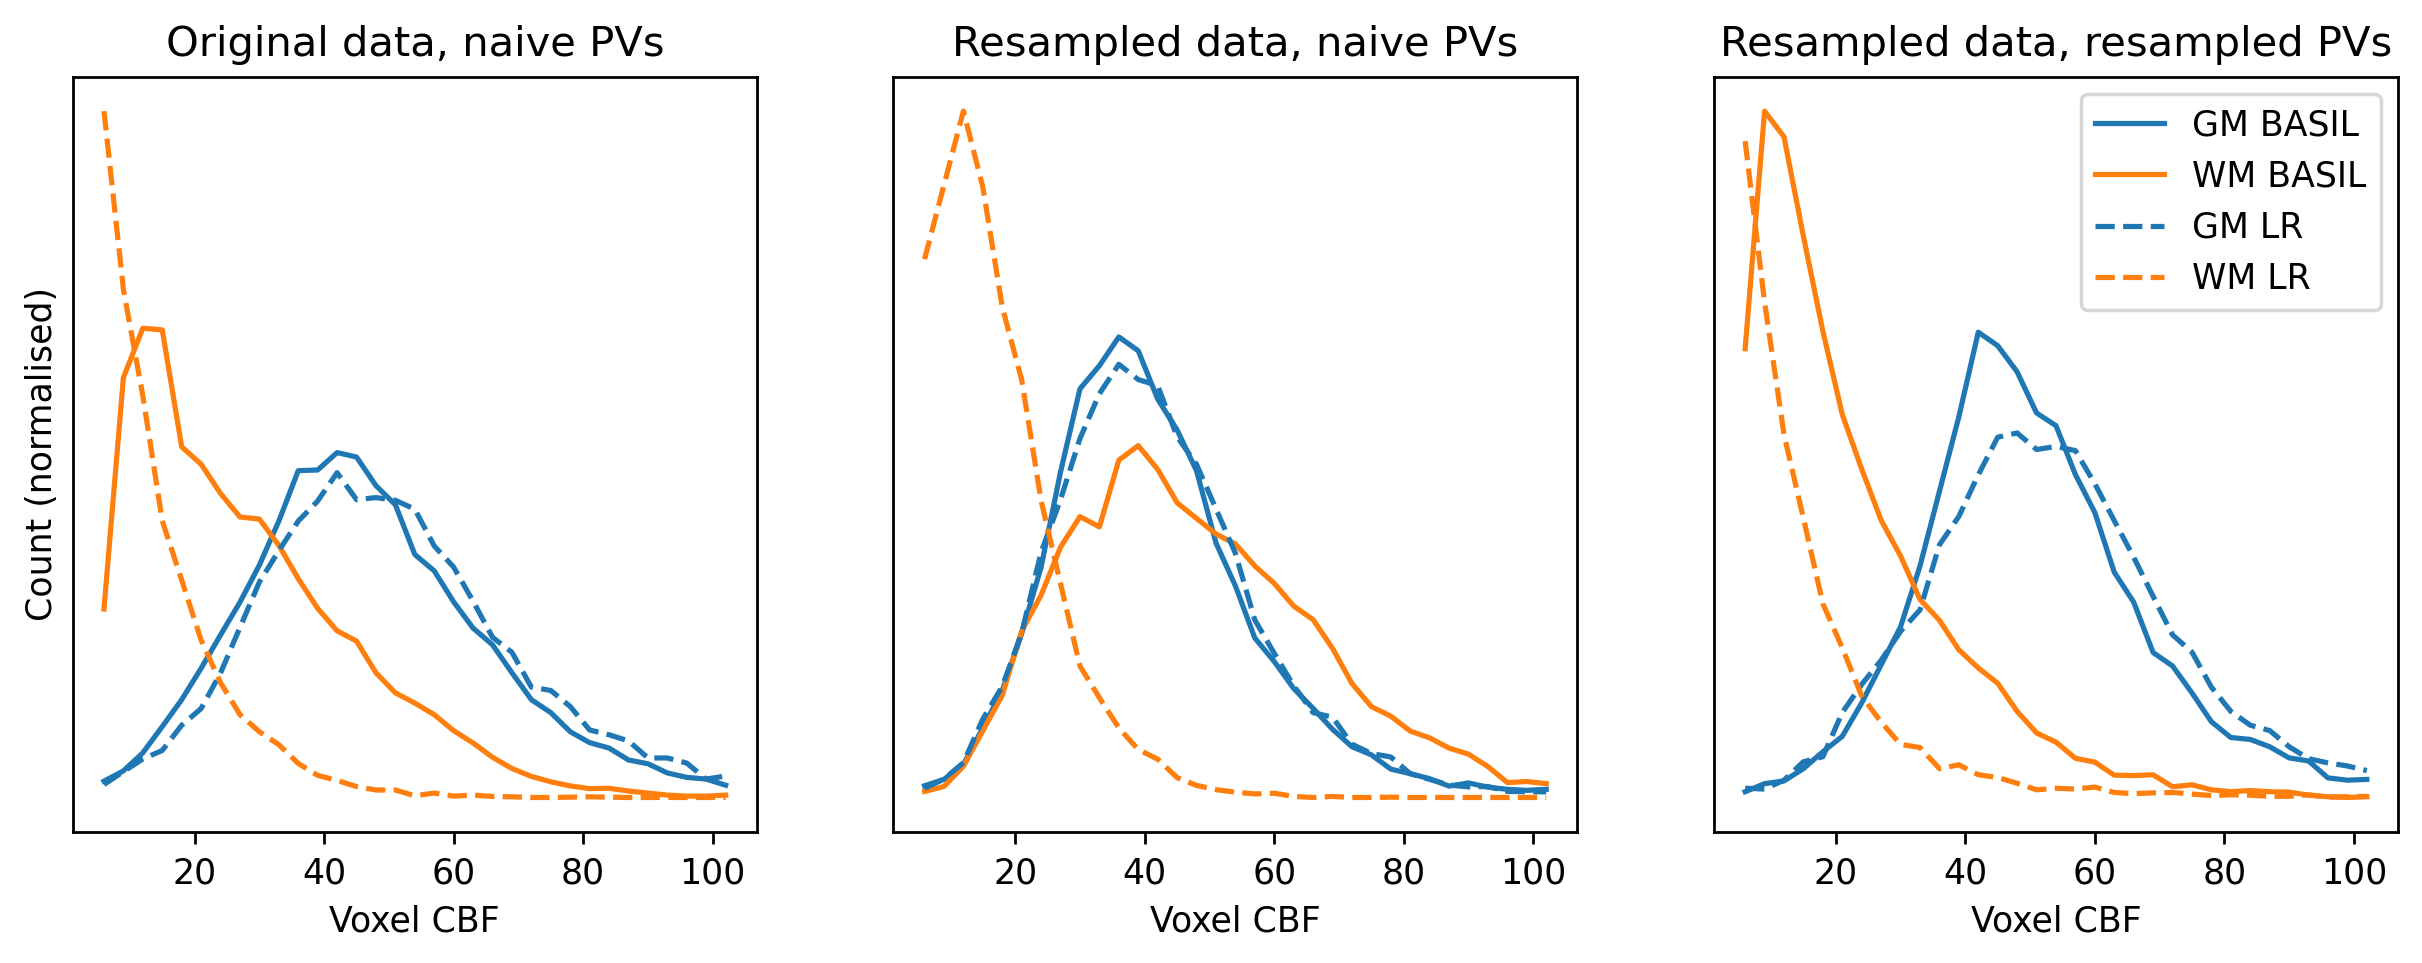
\includegraphics[width = \textwidth]{real_resamp_pvec.png}
\caption{Outcomes of PVEc before and after resampling. Left: original data with naive estimates; Centre: resampled data with naive estimates; Right: resampled data with resampled estimates. The former case (left) was taken to establish the baseline result; PVEc of resampled data with resampled PVs (right) led to a more similar result than with the naive estimates (centre).}
\label{real_resamp_pvec}
\end{figure}

Figure \ref{real_resamp_pvec} shows the outcomes of PVEc on the high SNR \textit{in-vivo} data before and after resampling. PVEc of the original data with the naive PVs established the expected distributions in the baseline case. PVEc of resampled data with naive PVs led to different distributions, particularly for BASIL's WM result which showed a positive skew. Both BASIL and the LR method returned a similar distribution for GM. PVEc of resampled data with resampled PVs resulted in distributions that more closely matched the baseline case (particularly for BASIL's WM result). These two findings (firstly, the choice of naive or resampled PVs affected the outcome of PVEc, and secondly, PVEc of resampled data with resampled PVs better matched the baseline case in native space), both matched the corresponding simulation results shown in figure \ref{sim_asl_resamp_pvec}. 


\begin{figure}[H]
\centering
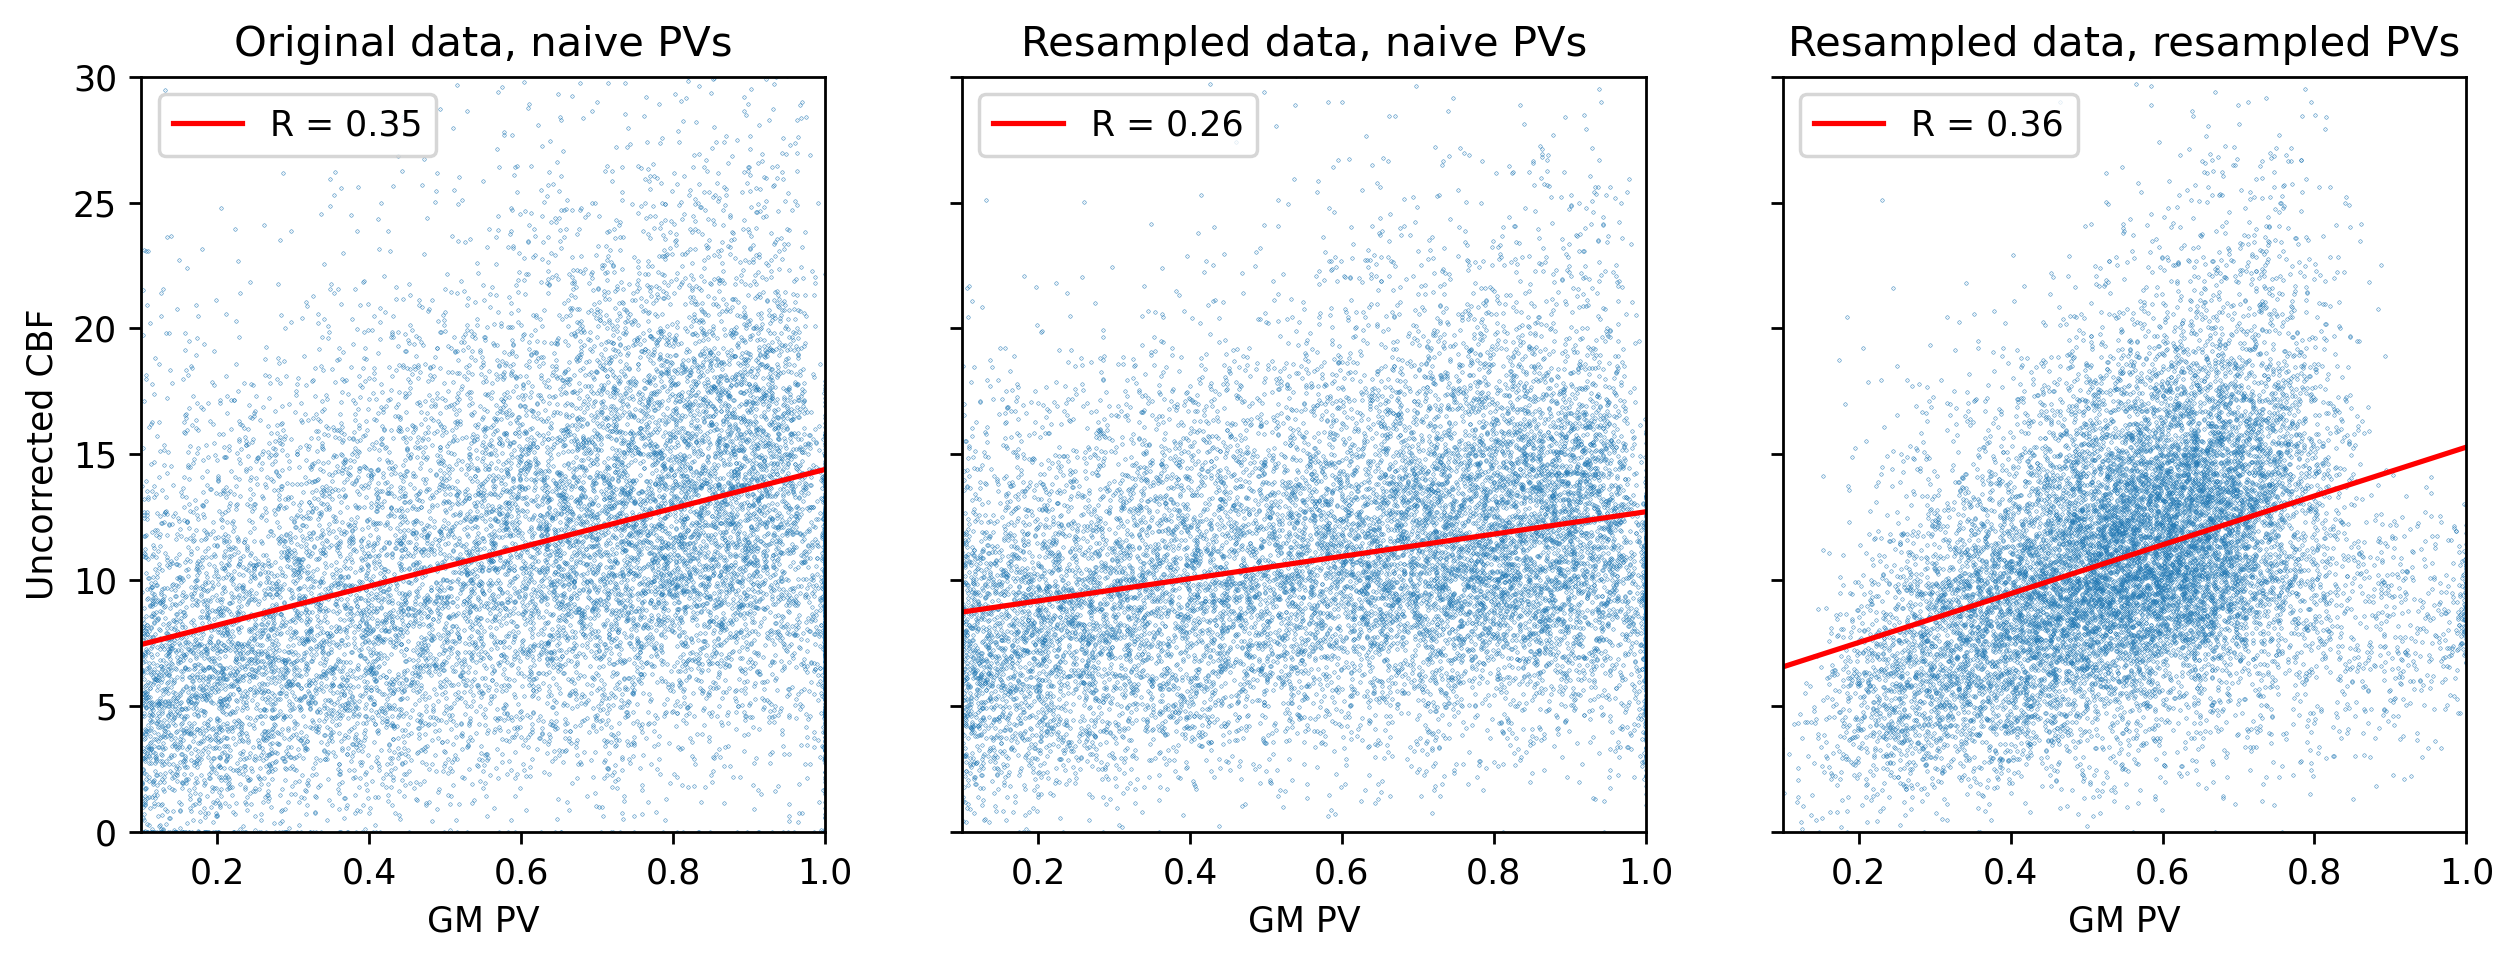
\includegraphics[width = \textwidth]{real_highsnr_scatter.png}
\caption{Scatter plots and linear regressions of uncorrected CBF estimated from data before and after resampling. Left: a scatter of the original data against the naive GM PV estimates established the baseline case, correlation coefficient $R$ = \DIFdelbeginFL \DIFdelFL{0.35}\DIFdelendFL \DIFaddbeginFL \DIFaddFL{0.34}\DIFaddendFL . Centre: a scatter of resampled data against the naive GM PVs resulted in a reduction of $R$ to \DIFdelbeginFL \DIFdelFL{0.26}\DIFdelendFL \DIFaddbeginFL \DIFaddFL{0.25}\DIFaddendFL . Right: a scatter of resampled data against resampled PVs showed an increase in $R$ to \DIFdelbeginFL \DIFdelFL{0.36}\DIFdelendFL \DIFaddbeginFL \DIFaddFL{0.31}\DIFaddendFL , \DIFdelbeginFL \DIFdelFL{matching }\DIFdelendFL \DIFaddbeginFL \DIFaddFL{closer to }\DIFaddendFL the baseline case.}
\label{real_highsnr_scatter}
\end{figure}

Figure \ref{real_highsnr_scatter} shows scatter plots and linear regressions of uncorrected CBF for the high SNR \textit{in-vivo} data before and after resampling. The regression of original data against the naive PVs established the baseline case with a correlation coefficient $R$ of \DIFdelbegin \DIFdel{0.35}\DIFdelend \DIFaddbegin \DIFadd{0.34}\DIFaddend . Regression of the resampled data against the naive PVs resulted in an $R$ value of \DIFdelbegin \DIFdel{0.26}\DIFdelend \DIFaddbegin \DIFadd{0.25}\DIFaddend , whereas regression of the resampled data against the resampled PVs resulted in an $R$ of \DIFdelbegin \DIFdel{0.36}\DIFdelend \DIFaddbegin \DIFadd{0.31}\DIFaddend . This indicated that the double-resampled PVs better matched the PVE that were embedded within the resampled ASL data, a finding in agreement with the simulations shown in figure \ref{sim_asl_resamp_scatter}. 

\begin{figure}[H]
\centering
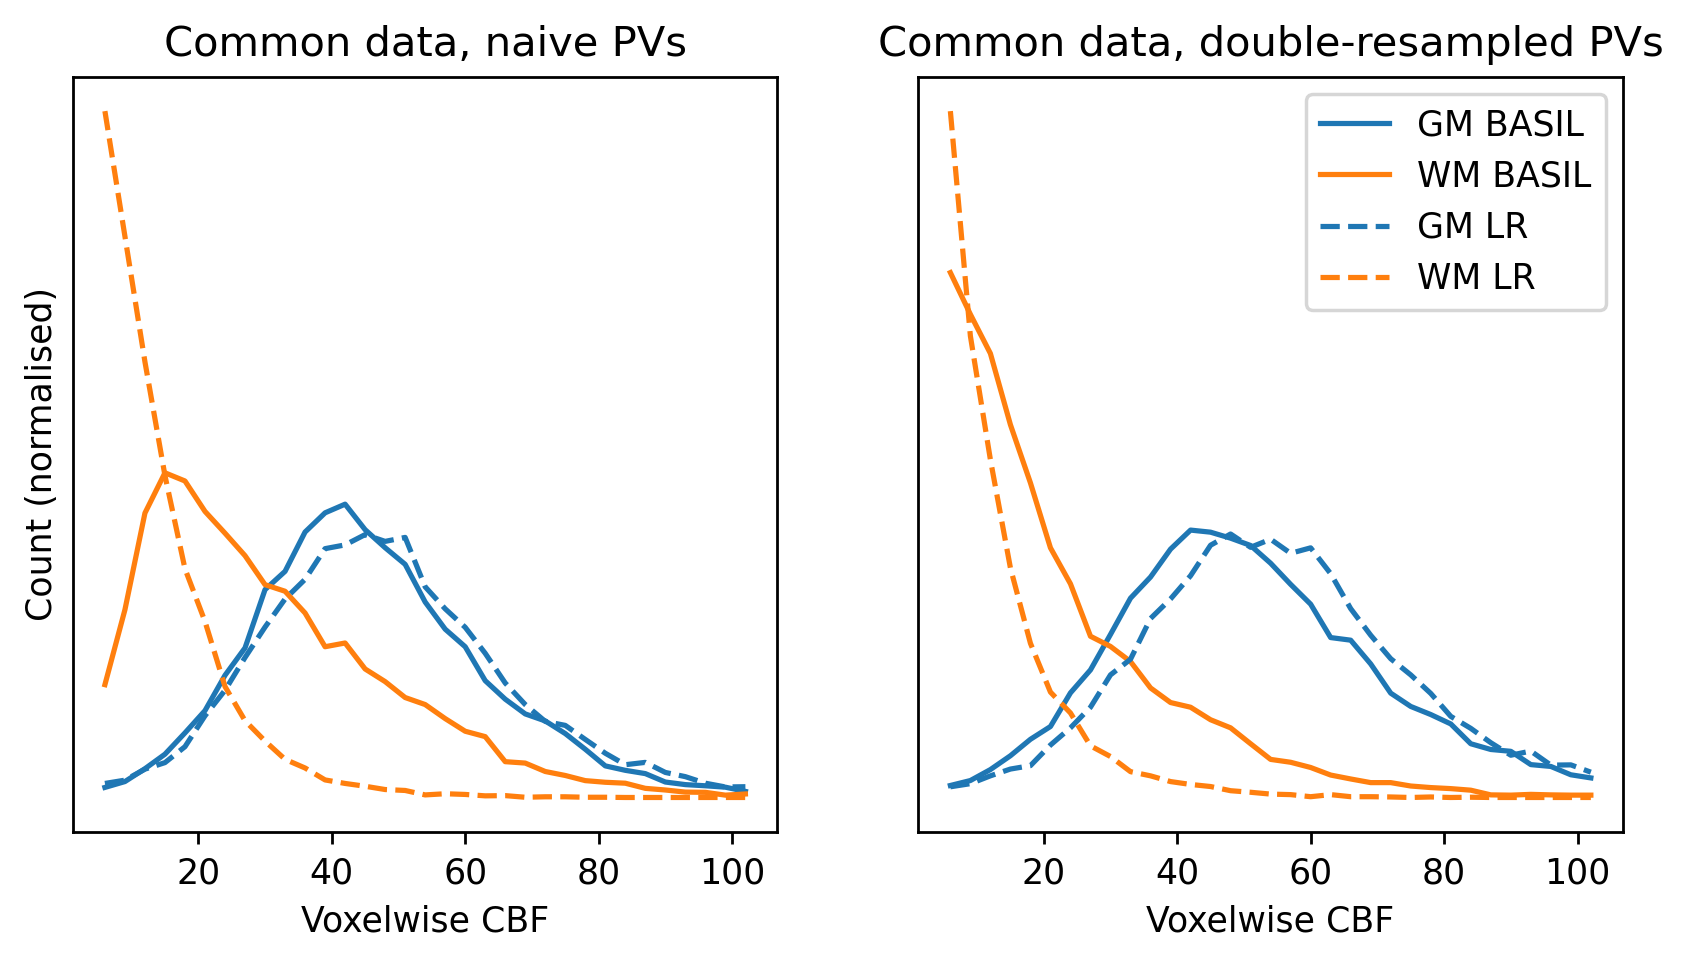
\includegraphics[width = 0.75\textwidth]{real_highsnr_pvec_cmn.png}
\caption{Outcomes of PVEc in common space, high SNR \textit{in-vivo} data. Left: PVEc with naive PV estimates. Right: PVEc with double-resampled PV estimates. Distributions of GM CBF were similar in either case. BASIL's WM distribution did alter noticeably;  double-resampled PVs led to better separation of tissue CBF compared to the naive case.}
\label{real_highsnr_pvec_cmn}
\end{figure}

Figure \ref{real_highsnr_pvec_cmn} shows the outcome of PVEc on the high SNR \textit{in-vivo} data after resampling into a common structural-aligned space. It is difficult to establish a baseline case in this situation because the ASL data has necessarily been resampled into a common space for analysis, thereby increasing the extent of PVE in the data in an unpredictable manner. BASIL's PVEc of the common aligned data with the naive PVs resulted in different distributions of GM and WM CBF than PVEc with the double-resampled PVs. In particular, PVEc with the double-resampled PVs resulted in better separation of the GM and WM CBF distributions for BASIL, a finding that matched the trends seen in acquisition-native space (figure \ref{real_resamp_pvec}).

\begin{figure}[H]
\centering
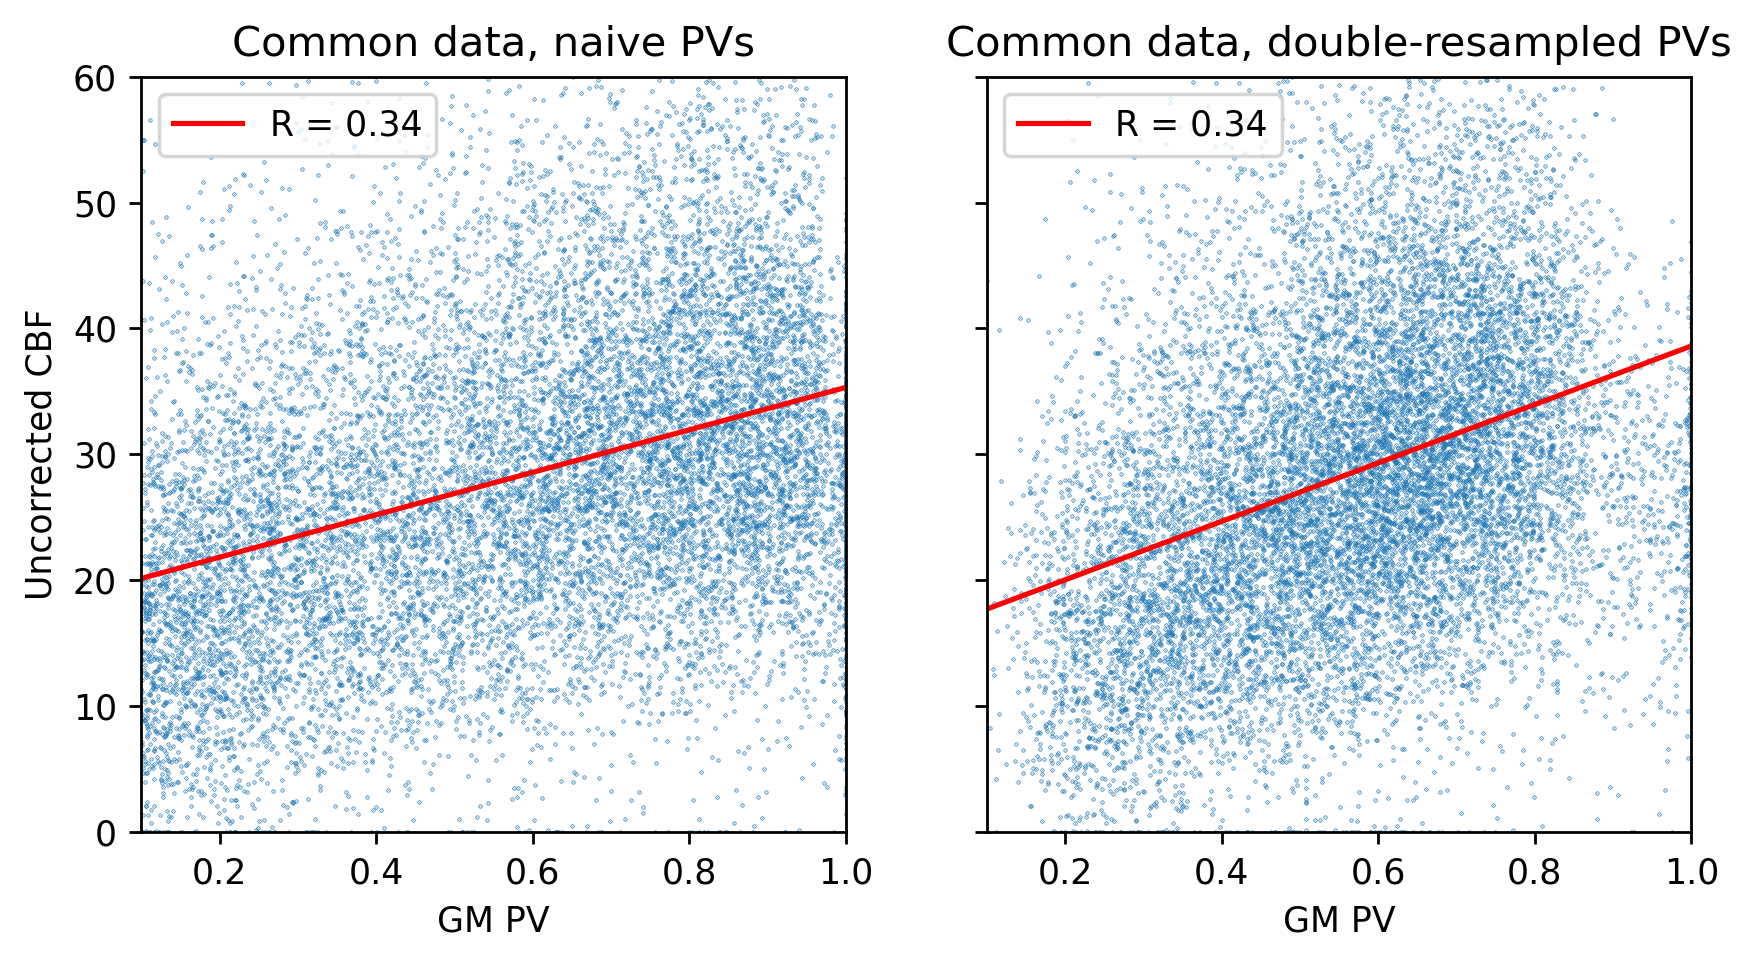
\includegraphics[width = 0.75\textwidth]{real_highsnr_scatter_cmn.png}
\caption{Scatter plots and linear regressions of uncorrected CBF in a common analysis space for the high SNR \textit{in-vivo} data. Left: regression against naive GM PV estimates. Right: regression against double-resampled GM PV estimates, with a slightly higher correlation coefficient (0.37 instead of 0.35).}
\label{real_highsnr_scatter_cmn}
\end{figure}

Figure \ref{real_highsnr_scatter_cmn} shows scatter plots and linear regressions of uncorrected CBF in a common analysis space estimated from the high SNR \textit{in-vivo} data. When regressed against the double-resampled GM PV estimates, there was a \DIFdelbegin \DIFdel{marginally higher }\DIFdelend \DIFaddbegin \DIFadd{no change in }\DIFaddend correlation coefficient ($R$ = \DIFdelbegin \DIFdel{0.37 instead of 0.35 with naive estimates}\DIFdelend \DIFaddbegin \DIFadd{0.34 in both cases}\DIFaddend ). 

%
%\begin{figure}[H]
%\centering
%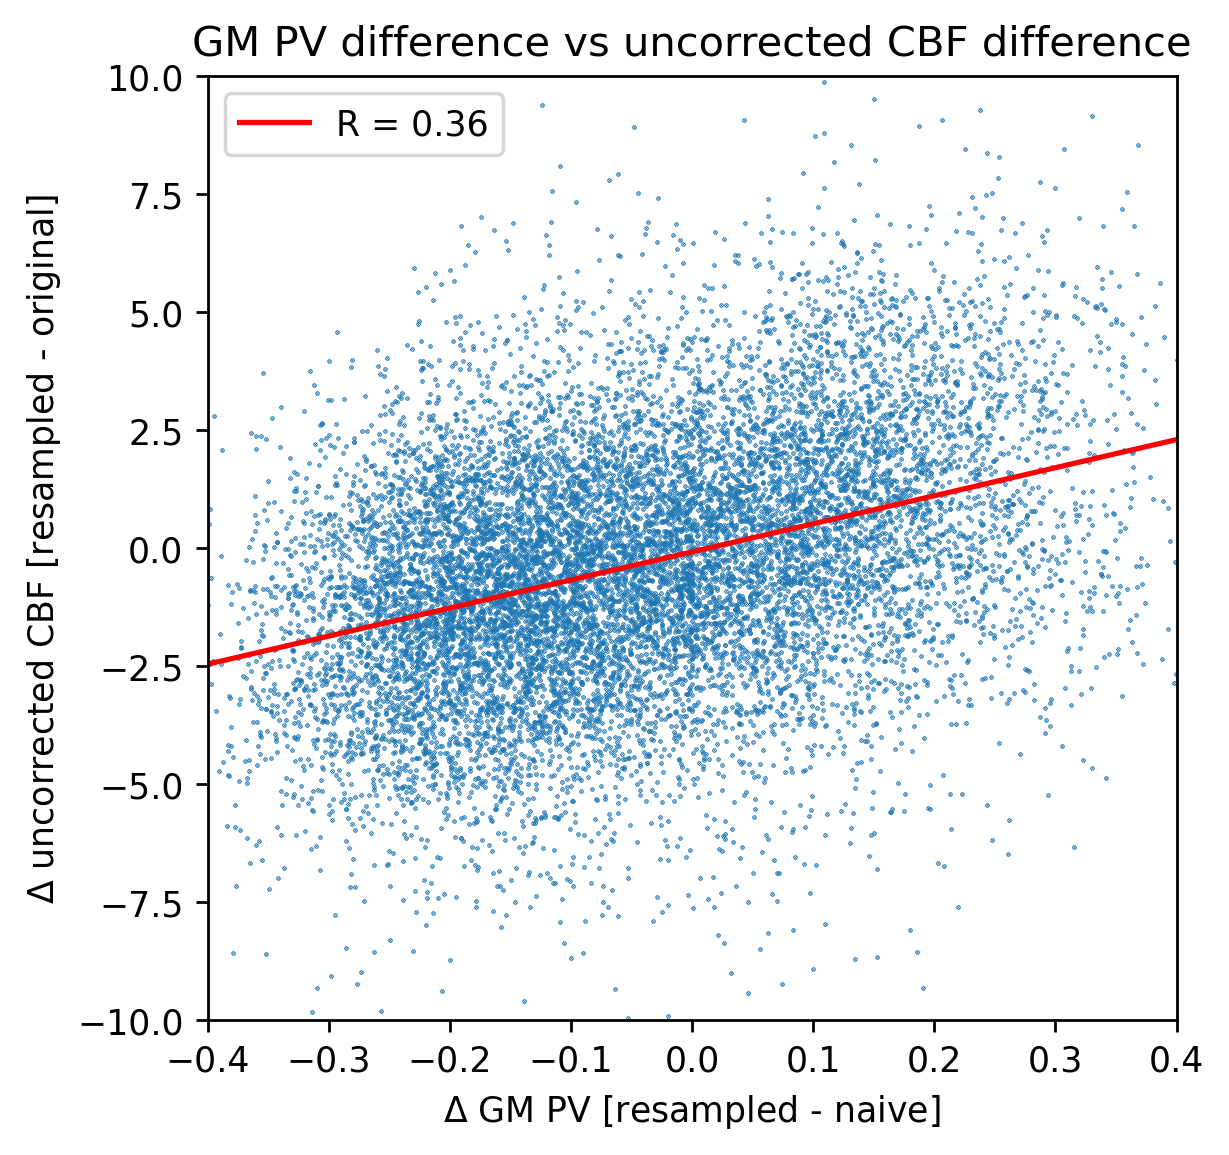
\includegraphics[width = 0.5\textwidth]{real_highsnr_deltagm_deltacbf.png}
%\caption{}
%\label{real_highsnr_deltagm_deltacbf}
%\end{figure}


\subsubsection{Low SNR repeats}


\begin{figure}[H]
\centering
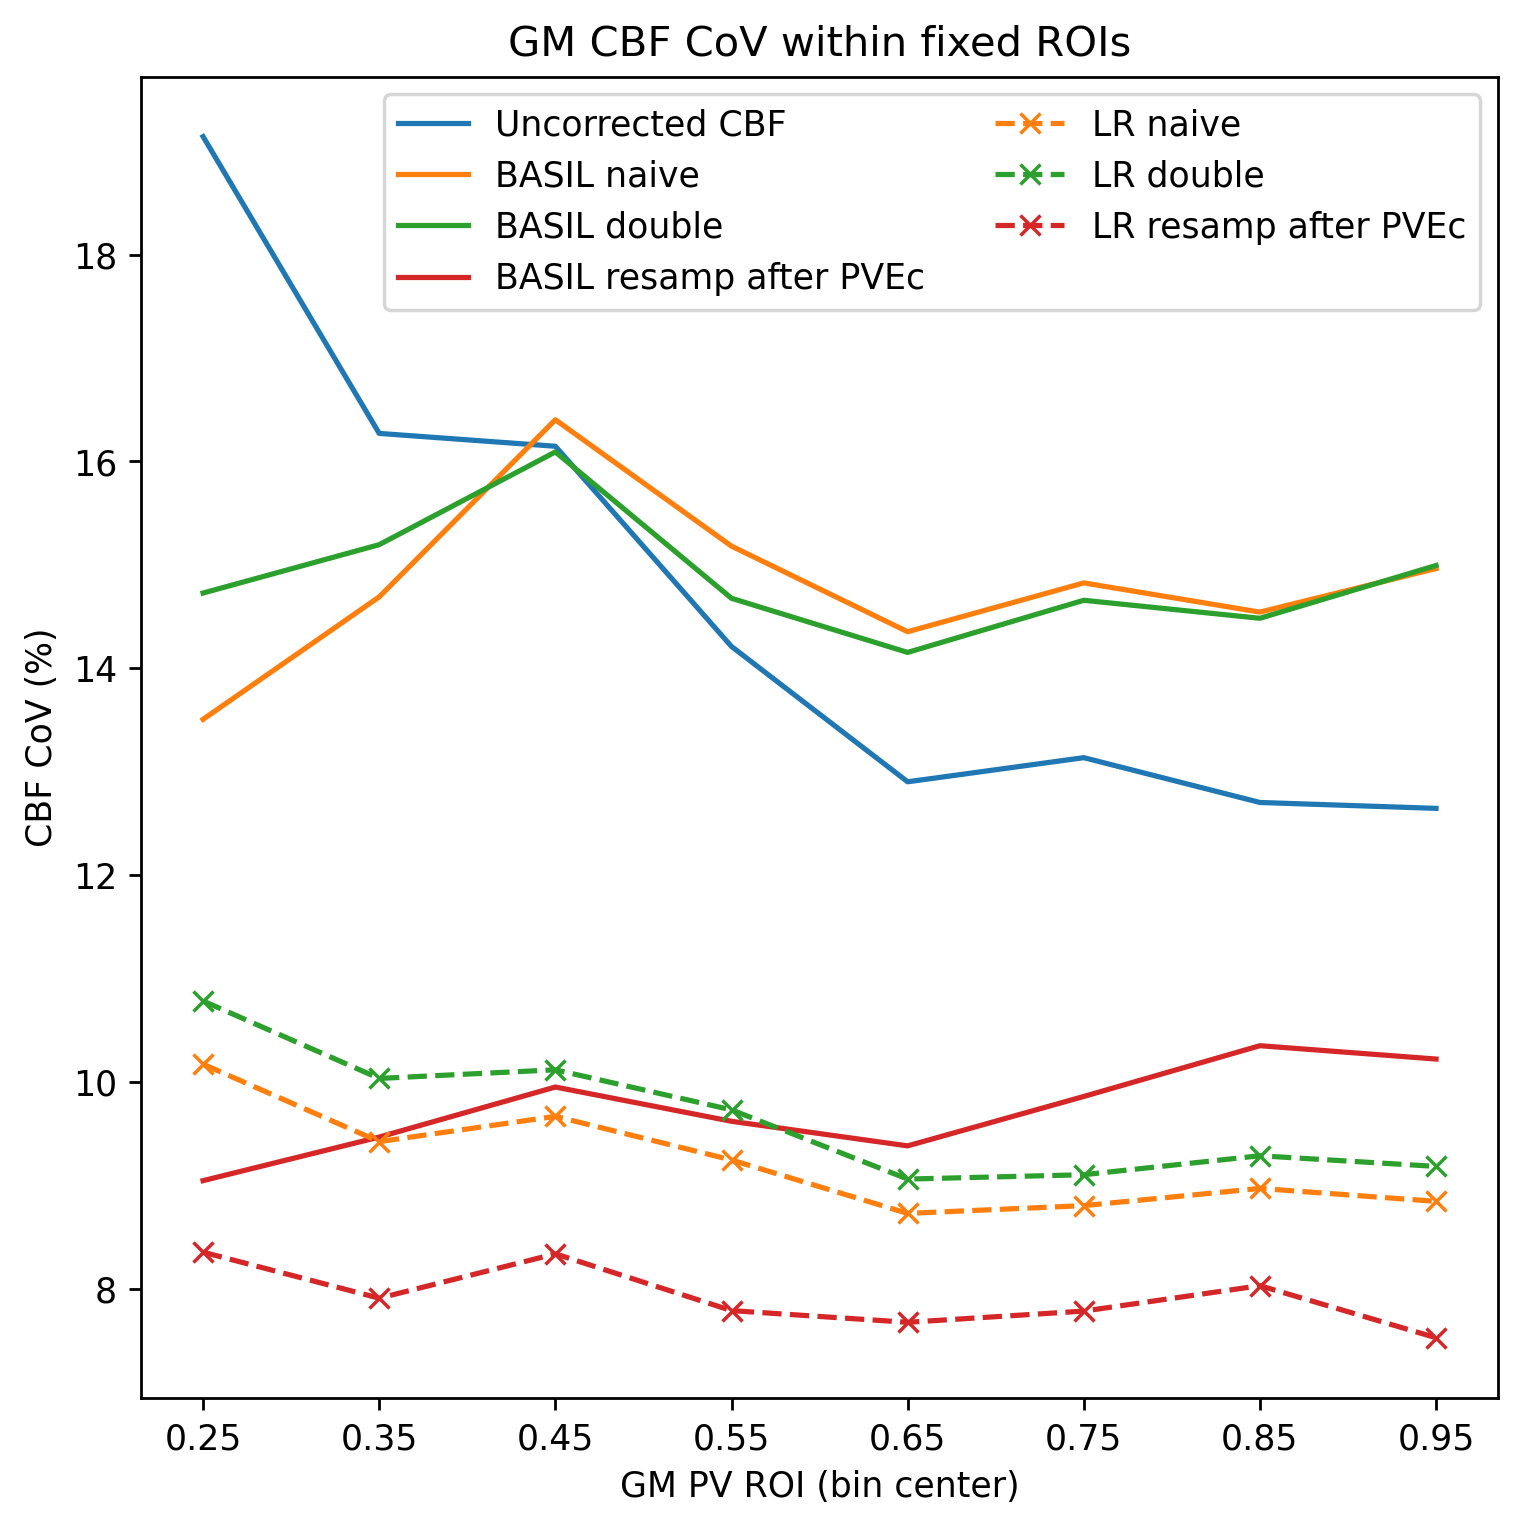
\includegraphics[width = 0.6\textwidth]{real_lowsnr_cov.png}
\caption{CoV in CBF measurement across the \textit{in-vivo} repeat data in common space. The trace of uncorrected CBF established the baseline case; CoV decreased with increasing GM PV. In general, LR methods returned substantially lower CoV than other methods, with the exception of BASIL resample after PVEc. The difference between naive (orange) and double-resampled (green) PVs was marginal for both the LR and BASIL methods. Resampling after PVEc gave the best performance for both PVEc methods.}
\label{real_lowsnr_cov}
\end{figure}

Figure \ref{real_lowsnr_cov} shows the CoV in CBF measurement across the \textit{in-vivo} repeat data in structural-aligned common space. The baseline case of uncorrected CBF was established; CoV decreased with increasing GM PV, in agreement with the simulated repeats (figure \ref{sim_lowsnr_cov}). All variants of the LR method returned substantially lower CoV than \DIFdelbegin \DIFdel{all }\DIFdelend \DIFaddbegin \DIFadd{the corresponding }\DIFaddend variants of BASIL\DIFdelbegin \DIFdel{, with the exception of BASIL resample after PVEc, which returned broadly similar results}\DIFdelend . For both the LR method and BASIL, the difference between correction with naive PV estimates or double-resampled estimates was marginal\DIFdelbegin \DIFdel{. Within each PVEc method, the strategy of resampling after PVEc led to the lowest CoV values}\DIFdelend \DIFaddbegin \DIFadd{, however there was a clear reduction in CoV when using the resample after PVEc strategy}\DIFaddend . 

\section{Discussion}

It is well known that resampling has the effect of smoothing data. This also increases the extent of PVE, which was readily observed in distributions of uncorrected CBF (figures \ref{sim_asl_resamp_hist} and \ref{real_resamp_hist}). The smoothing imposed by resampling also had a small noise-reducing effect which could be observed on the simulation experiments. Referring to the scatter plots in figure \ref{sim_asl_resamp_scatter}, the bimodal distribution of the original data resulted in two distinct linear clusterings, and the amount of noise was reflected in the spread of points around these clusterings. Following resampling, a bimodal distribution was again observed, but the spread of points around the clusterings was reduced, indicative of reduced noise within the data. 

If PVE are known to be present in the data, the results presented here imply native-space parameter estimation is preferable so as to avoid resampling which further increases PVE\DIFaddbegin \footnote{\DIFadd{It is acknowledged that motion correction, which is highly desirable for timeseries data, will entail an unavoidable interpolation step. Nevertheless, with careful workflow design the impact of this can be minimised.}}\DIFaddend . There may of course be other justifications for analysing data in a non-native space that outweigh the importance of PVE. In such a situation, results from the simulations showed that PVEc with the double-resampling strategy was more successful than using naive PV estimates (figure \ref{sim_rpts_resamp_pvec}), but this result relied on the wholly unrealistic assumption of constant CBF in each tissue. For \textit{in-vivo} data, the difference between the naive and double-resampled strategies was more marginal, but the latter strategy nevertheless led to better separation of GM and WM CBF distributions (figure \ref{real_highsnr_pvec_cmn}) and a higher correlation coefficient of GM PV with uncorrected CBF (figure \ref{real_highsnr_scatter_cmn}). As such, it is concluded that obtaining PV estimates via double-resampling represents the best strategy for PVEc in non-native data space, but is nevertheless a compromise compared to native space parameter estimation. 

The reasoning behind the success of the double-resampled strategy is that it redistributes PVs between voxels in the same manner as signal is redistributed within the data that is being resampled. In this regard, one can draw a parallel with the emphasis placed on PSF-related effects in the PET PVE literature: resampling increases the effective PSF of data such that mixing of signal between voxels becomes problematic. Ironically, the importance of this result may actually increase as voxel size decreases, up to a point. Considering the example of a simple translation, for a fixed displacement of 1mm the amount of smoothing introduced when applied to a 2mm voxel grid would be greater than for a 4mm voxel grid (due to subvoxel effects, as illustrated in figure \ref{resamp_demo}). Hence, the resampling necessitated by a given transformation is more detrimental when applied to high resolution data than for low resolution. An alternative formulation is that data with low PVE stands to lose more information than data that contains high PVE; if one goes through the effort of obtaining data with low PVE, then one should strive to preserve that as much as possible during processing. 

In general, the results drawn from the \textit{in-vivo} data are harder to interpret because it is not known ahead of time what the `correct' result would look like. For example, the simulations used an assumption of constant CBF in both tissues so as to ensure any variance in CBF measurement could be explained by PVE. This clearly does not hold true for \textit{in-vivo} data. This likely explains, along with greater noise, why correlation coefficients of GM PV against uncorrected CBF (figure \ref{real_highsnr_scatter}) were lower across the board than for the simulation experiments. As for the repeatability of CBF measurement in repeat data, a minimal coefficient of variation cannot necessarily be assumed to be the correct result: there may have been genuine physiological change in CBF between the repeat measurements, hence implying the true CoV would be non-zero. Both simulations and theory suggested that because the double-resampled PVs conveyed more meaningful information about the PVE of resampled data, and therefore enabled better PVEc, they should have resulted in reduced CoV for common-space CBF measurements. In fact, the difference versus the naive PV estimates on the \textit{in-vivo} repeat data was marginal at best (figure \ref{real_lowsnr_cov}). More intriguingly, BASIL's PVEc with either the naive or double-resampled strategy resulted in a higher CoV than doing no PVEc at all \DIFaddbegin \DIFadd{in many ROIs}\DIFaddend ; only BASIL's `resample after PVEc' was able to \DIFaddbegin \DIFadd{consistently }\DIFaddend reduce CoV below that of no correction. This suggests that the emphasis placed on PVEc within the ASL literature as a means of improving the repeatability of CBF measurement needs careful qualification: PVEc \textit{can} reduce CoV of repeat measurements, but the specifics of implementation are all-important. Here, \DIFdelbegin \DIFdel{a naive approach }\DIFdelend \DIFaddbegin \DIFadd{two variants of PVEc with BASIL }\DIFaddend in fact increased CoV for \textit{in-vivo} data (figure \ref{real_lowsnr_cov}). 

Dissecting the results of CoV in CBF measurement from the \textit{in-vivo} repeat data in more detail (figure \ref{real_lowsnr_cov}), all variants of the LR method returned relatively similar CoV values in all ROIs. This suggests that the level of smoothing imposed by the LR method is both relatively high and also insensitive to the PV estimates themselves (hence the marginal difference between double-resampled and naive PV estimates). On the \DIFdelbegin \DIFdel{simulated }\DIFdelend \DIFaddbegin \textit{\DIFadd{simulated}} \DIFaddend repeat data (figure \ref{sim_lowsnr_cov}), BASIL returned very different results for the double-resampled and naive strategies, so it can be sensitive to PV estimates in the general case, but this did not hold true with this specific \textit{in-vivo} data. The contradiction is likely explained by the nature in which BASIL determines the optimal level of smoothing to apply to data (and by extension condition the system of equations that must be solved as part of PVEc). Unlike the LR method, the level of smoothing is not a property that is fixed ahead of time by the kernel size and is instead determined from the data itself. A trend that was frequently observed during the development of this work was that BASIL applied higher levels of smoothing to data that was fundamentally smooth in the first place, because there was no penalty to doing so (in the Bayesian terminology, the data supported a high level of smoothing). The reverse was true on data that was not smooth, or data that was very noisy. It is suspected that this behaviour explains the relatively high and similar CoV returned by BASIL for the naive and double-resampled strategies in figure \ref{real_lowsnr_cov}: although the double-resampled PVs may be more informative than the naive PVs, the low data quality does not support a high enough level of smoothing on the data to achieve successful PVEc, hence both PV estimates lead to a similar outcome (that is in fact generally worse than doing no PVEc). 

The low CoV values returned by both variants of the `resample after PVEc' strategy on the \textit{in-vivo} repeat data (figure \ref{real_lowsnr_cov}) point back to the overriding conclusion that can be drawn from this work: parameter estimation in native space is preferable, because any prior resampling step introduces extra PVE that cannot be fully accounted for in subsequent PVEc \DIFaddbegin \DIFadd{(even with the double resampling strategy)}\DIFaddend . Therefore, if common space analysis is required, the repeat data should be processed with PVEc in its native space and then the outputs (CBF maps) transformed into common space. Although this still involves a resampling operation, the key difference is that resampling the PVEc output maps does not introduce extra PVE into the data, because such maps only contain a single tissue signal in the first place (\textit{e.g.}, GM CBF), not mixed tissue signals. This is not true of the actual ASL data \textit{prior} to CBF estimation and PVEc. 
\DIFdelbegin \DIFdel{In light of this, the low CoV returned by this strategy on the }\DIFdelend \DIFaddbegin 

\DIFadd{Though the }\DIFaddend \textit{in-vivo} \DIFdelbegin \DIFdel{data is in accordance with expectations (figure \ref{real_lowsnr_cov}), though the relatively high CoV returned by this strategy on the simulated repeat data is a more puzzling (figure \ref{sim_lowsnr_cov}). It is strongly suspected that the latter result was }\DIFdelend \DIFaddbegin \DIFadd{results presented here are drawn off a small dataset acquired with non-typical parameters (7T pASL), it is reasonable to assume they would hold with other acquisition schemes and field strengths. This is because the mechanism that has been investigated here (the interaction between PVE and resampling) is independent of acquisition specifics and arises }\DIFaddend due to the \DIFdelbegin \DIFdel{combination of noise reduction imparted by resampling the ASL data into common space and the assumption of constant CBF in each tissue leading to an exceptionally favourable scenario for PVEc. As both PVEc methods investigated here make the same underlying assumption of constant CBF within local voxel neighbourhoods}\DIFdelend \DIFaddbegin \DIFadd{data processing operations that are common to all ASL analyses. Nevertheless, it is possible to question the }\textit{\DIFadd{relative}} \DIFadd{importance of these results in the general case: there are many competing challenges when analysing ASL data, and it may be that PVE are of minor importance for a given study objective. Overall}\DIFaddend , it is \DIFdelbegin \DIFdel{expected that the combination of low noise with genuinely constant underlying CBF in the data leads to an extremely low CoV, whereas the estimation in native space had to contend with higher noise. The }\textit{\DIFdel{in-vivo}} %DIFAUXCMD
\DIFdel{data almost certainly does not lead to the same serendipitous circumstances (CBF is not constant), hence PVEc after resampling is not so favourable}\DIFdelend \DIFaddbegin \DIFadd{hoped that the findings of this work are sufficiently easy to implement (in essence, a simple re-arrangement of the order in which data processing is performed, and requiring no new tools) that they can be adopted without impacting other analysis objectives}\DIFaddend . 

\section{Conclusion}

This work has investigated the origin and impacts of PVE on physiological imaging data. Particular emphasis has been placed onto how PVE interact with common data processing operations (registration, transformation, resampling and interpolation) in the course of an analysis pipeline. It has been shown that PVE are not fixed once and for all at the time of data acquisition but are in fact modified by subsequent data processing (there is an analogy with entropy, in that these operations strictly increase PVE). A number of simple but easy-to-implement conclusions can be drawn from this. 

Firstly, for data that is known to contain PVE, parameter estimation in native data space is preferable as this offers the best chance of performing PVEc. If spatial correspondence in a common analysis space (whether within or between subjects) is required, then transformation of \DIFdelbegin \DIFdel{PVEc }\DIFdelend \DIFaddbegin \DIFadd{PVE corrected }\DIFaddend output parameter maps is preferred over transformation of the underlying data itself. This is because transforming the output maps does not lead to mixing of tissue signal between voxels. If it is not possible to abide by the previous two recommendations, then performing PVEc of transformed data using the double-resampling strategy (estimating PVs first in native data space, and then applying the same set of transformations into analysis space as for the data itself) offers the best chance of performing successful PVEc. Finally, regarding the potential benefits of PVEc for improving the repeatability of analysis in a common space, it has been shown that such an outcome is highly sensitive to the specifics of implementation. For BASIL in particular, PVEc of any variant on resampled \textit{in-vivo} data often led to increased CoV in CBF measurement compared to no correction; only PVEc on the native space data \textit{before} transformation of the results into common space was able to reduce CoV compared to no correction. Though the differences between these various strategies as exhibited on \textit{in-vivo} data tended to be small, the strategies are nevertheless simple to implement (requiring no new tools or methods) and offer a pragmatic means of maximising the utility of data in the face of numerous other analysis challenges. 

 \newpage 
 \newpage % Activate the following line by filling in the right side. If for example the name of the root file is Main.tex, write
% "...root = Main.tex" if the chapter file is in the same directory, and "...root = ../Main.tex" if the chapter is in a subdirectory.

% !TEX root = ../thesis.tex 

\chapter[Surface-based PV estimation]{Surface-based partial volume estimation}
\label{tob_pv_chapter}

\section{Introduction}

Although surface-based segmentation is well-established within the literature, the same is not true of surface-based PV estimation\footnote{The majority of the work presented in this chapter has been published as T. Kirk, T. Coalson, M. Craig and M. Chappell, ``Toblerone: surface-based partial volume estimation'', IEEE Transaction on Medical Imaging, vol. 39 no. 5, pp 1501 - 1510, 2020.}. A surface-based approach could bring two key advantages. Firstly, if it is true that surface segmentations of particular structures are more accurate than their volumetric counterparts, then the same could also be true of PV estimates derived from these (although the accuracy of any such estimates will be constrained by that of the surfaces from which they are derived). This would in turn have implications \DIFdelbegin \DIFdel{of }\DIFdelend \DIFaddbegin \DIFadd{for }\DIFaddend the efficacy of PVEc within these structures. Secondly, a surface-based approach allows PVs to be obtained in any voxel grid without recourse to resampling. This is beneficial for minimising the mixing of signal that is introduced by resampling, an artefact that cannot be fully accounted for by subsequent correction (as was demonstrated in chapter \ref{pvec_chapter}). 

Conceptually, surface-based PV estimation approaches the problem in a purely geometric manner: \textit{given a patch of surface that intersects a voxel, what is the volume on either side of the surface that is bounded by the voxel?} It is this formulation that makes the approach immune to the problems of resampling. For a given surface intersecting a voxel grid, any transformation can be performed by manipulating the voxel grid (for example, a translation, rotation or scaling) independent of the surface itself. This means that the boundaries of the anatomical structure represented by the surface are conserved. This same is not true of a volumetric approach: in that case, the boundaries of the structure have been reduced to a voxel-wise representation (the result of volumetric segmentation), and therefore any transformation operation must be applied to the voxel representation of the structure, which will in turn entail interpolation across structure boundaries at the cost of edge definition. The consequences of this are illustrated in greater detail in figure \ref{resampling_demo}. 

\begin{figure}
\centering
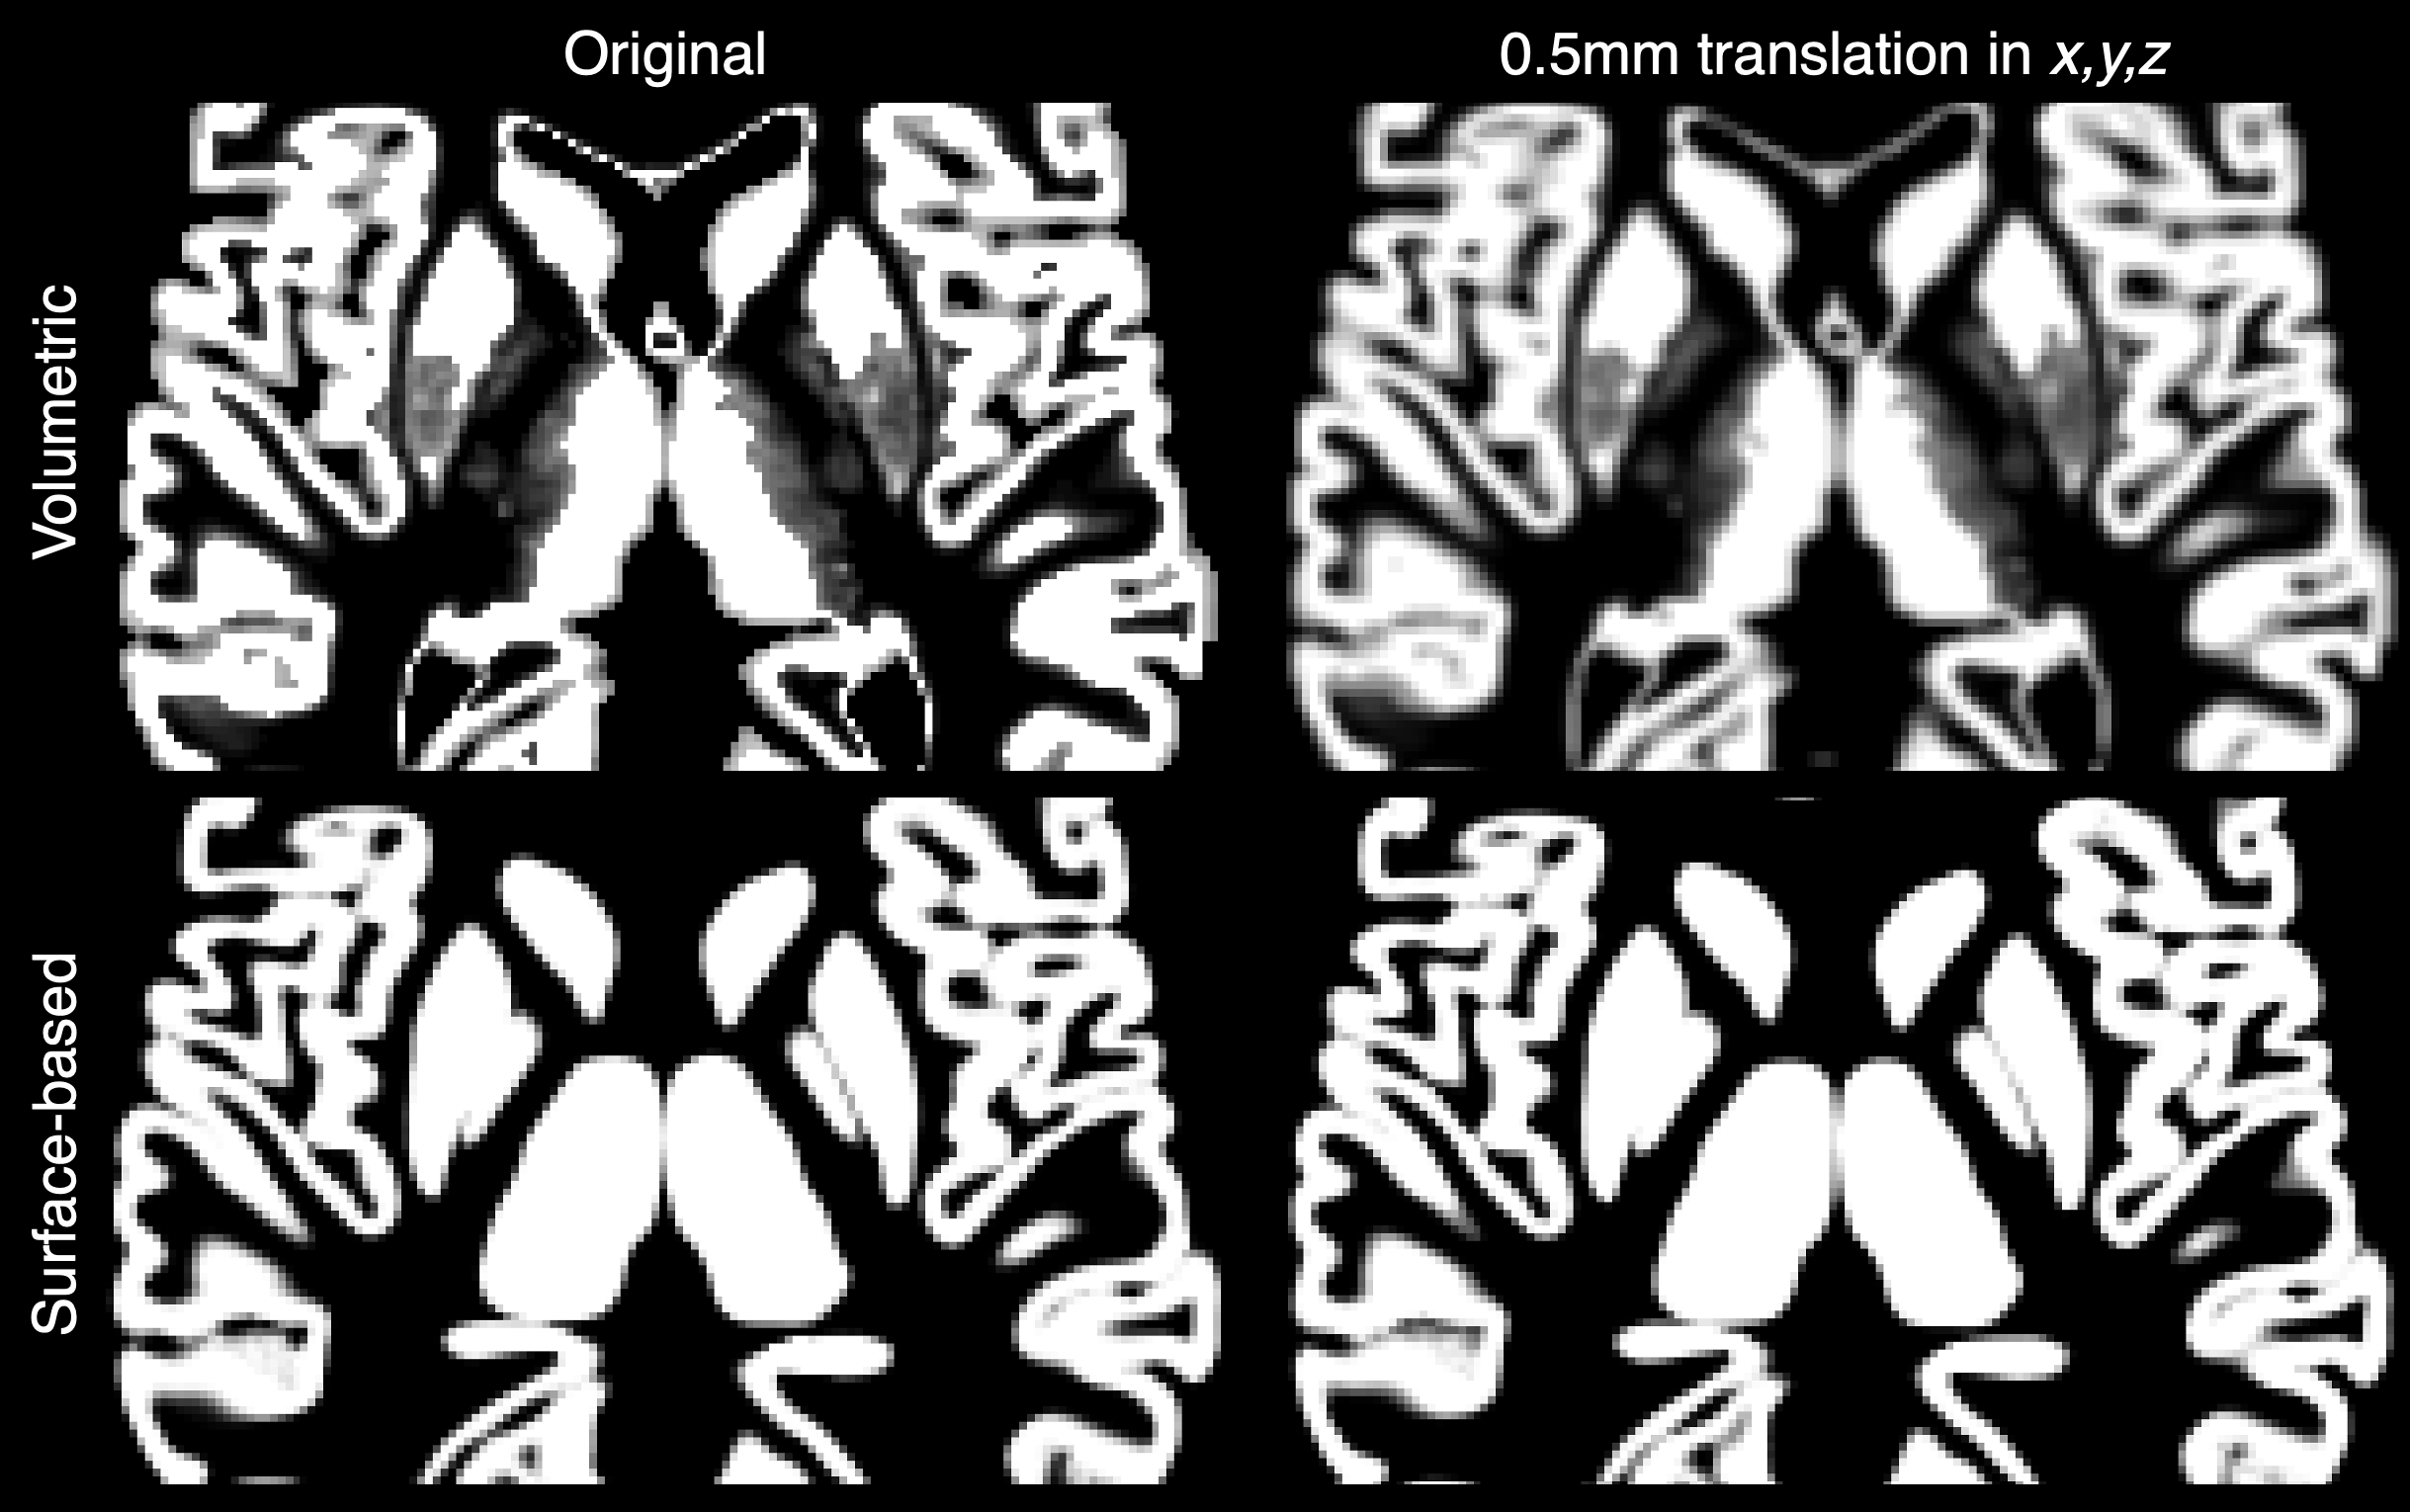
\includegraphics[width = \textwidth]{resampling.png}
\caption{Illustration of resampling-induced blurring on a 1mm isotropic GM PV map. The left column shows the original estimates produced by a volumetric method (FSL FAST) and a surface-based method (Toblerone, the subject of this chapter); the right shows the result of a 0.5mm translation along each axis. For a volumetric method, any transformation will require a resampling operation that blurs the boundaries of underlying structure. For a surface-based method, the same transformation can be achieved by manipulating the voxel grid independently of the surface itself, hence avoiding resampling and the accompanying blurring.}
\label{resampling_demo}
\end{figure}

Although some surface-based PV estimation tools exist in the literature, past efforts have usually been designed with a specific modality in mind. Two notable examples for neuroimaging are the ribbon-constrained (RC) method used within the HCP's \textit{fMRISurface} pipeline \cite{Glasser2013} and PETSurfer \cite{Greve2016, Greve2014}, a variant of FreeSurfer. The former is designed for use with BOLD and so distinguishes only between cortex and otherwise, not the GM, WM and non-brain required by other modalities; whereas the latter is both PET-specific and tightly integrated into FreeSurfer such that it is hard to use independently of that workflow. One of the few examples of a generally applicable method that is not tied to any particular modality is NeuropolyPVE, though that is also constrained to use with the cortex only \cite{NeuropolyPVE}. \DIFaddbegin \DIFadd{It should also be noted that FreeSurfer itself, which is widely used to generate the surfaces on which these methods operate, does offer some tools to perform surface-based PV estimation for the cortex only (and not the subcortex). It is however somewhat difficult to use the outputs of these tools independently of the wider FreeSurfer workflow, which means they are awkward to integrate into a general purpose analysis pipeline with PVEc. 
}\DIFaddend 

The objective of this work was to develop an algorithm, named Toblerone, to estimate partial volumes for both cortical and subcortical structures (where such surfaces are available, for example via FSL FIRST \cite{Patenaude2011}) for neuroimaging applications. The end result is highly general and could be used with data from multiple modalities and/or in other parts of the body. 

\section{Theoretical foundation}

Voxelisation is the process of quantifying the volume contained within a surface and many algorithmic implementations are given in the computer graphics literature. The key step within this operation is determining if a point lies interior or exterior to a given surface; by repeating this test entire volumes can be built up. The ray intersection test outlined by Nooruddin and Turk is widely used for this and requires only that the surfaces be contiguous (water-tight) \cite{Nooruddin2003}. The test is performed by projecting an infinite ray in any direction from the point under test and counting the number of intersections made with the surface. A ray from an interior point will make an odd number of intersections as it exits the surface (including folds within the surface, there will be one more point of exit than entry); conversely an exterior point will make an even number of intersections (balanced entries and exits), if at all. This test scales badly with increasing spatial resolution: for a linear resolution of $n$ samples per unit distance, $n^3$ tests per unit volume are required. Furthermore, as each ray must be tested against each surface element, the test also becomes more complex for increasing surface resolution (linearly for a naïve implementation). For a typical functional image of 10\textsuperscript{5} voxels and 2.5x10\textsuperscript{5} surface elements in a FreeSurfer cortical surface, this is prohibitively computationally intensive.

The method adopted in this work is to only use the portion of surface that actually intersects a given voxel (termed the \textit{local patch}) for ray intersection testing. The local patch is defined as all triangles that intersect the voxel or, equivalently, the minimal set of triangles that unambiguously divides the voxel into two regions. This patch is by definition non-contiguous, so it is necessary to modify the ray intersection test accordingly; the modified form is referred to as the ‘reduced’ test in contrast to the ‘classical’ test. Within each voxel, a \textit{root point} that is known to lie within the surface is identified via the classical ray test. Any other point within the voxel may then be tested by projecting the finite line segment 

\begin{equation}
\vec{r} = \vec{p_t} + \lambda(\vec{p_r} - \vec{p_t})
\end{equation} 

where $\vec{p_t}$ is the point under test, $\vec{p_r}$ is the root point and $0 \leq \lambda \leq 1$ is a distance multiplier along the line. A parity test is then applied to the number of intersections identified between the root and test points. The fact that the line terminates at a point interior to the surface means that exterior points will lead to one more point of entry than exit; conversely interior points will lead to either zero or an even number of intersections. It is not necessary to test surface elements outside the voxel as the finite length of the line segment means it can never leave the voxel. Figure \ref{raytest} provides an illustration of the test in practice. 

\begin{figure}
\centering
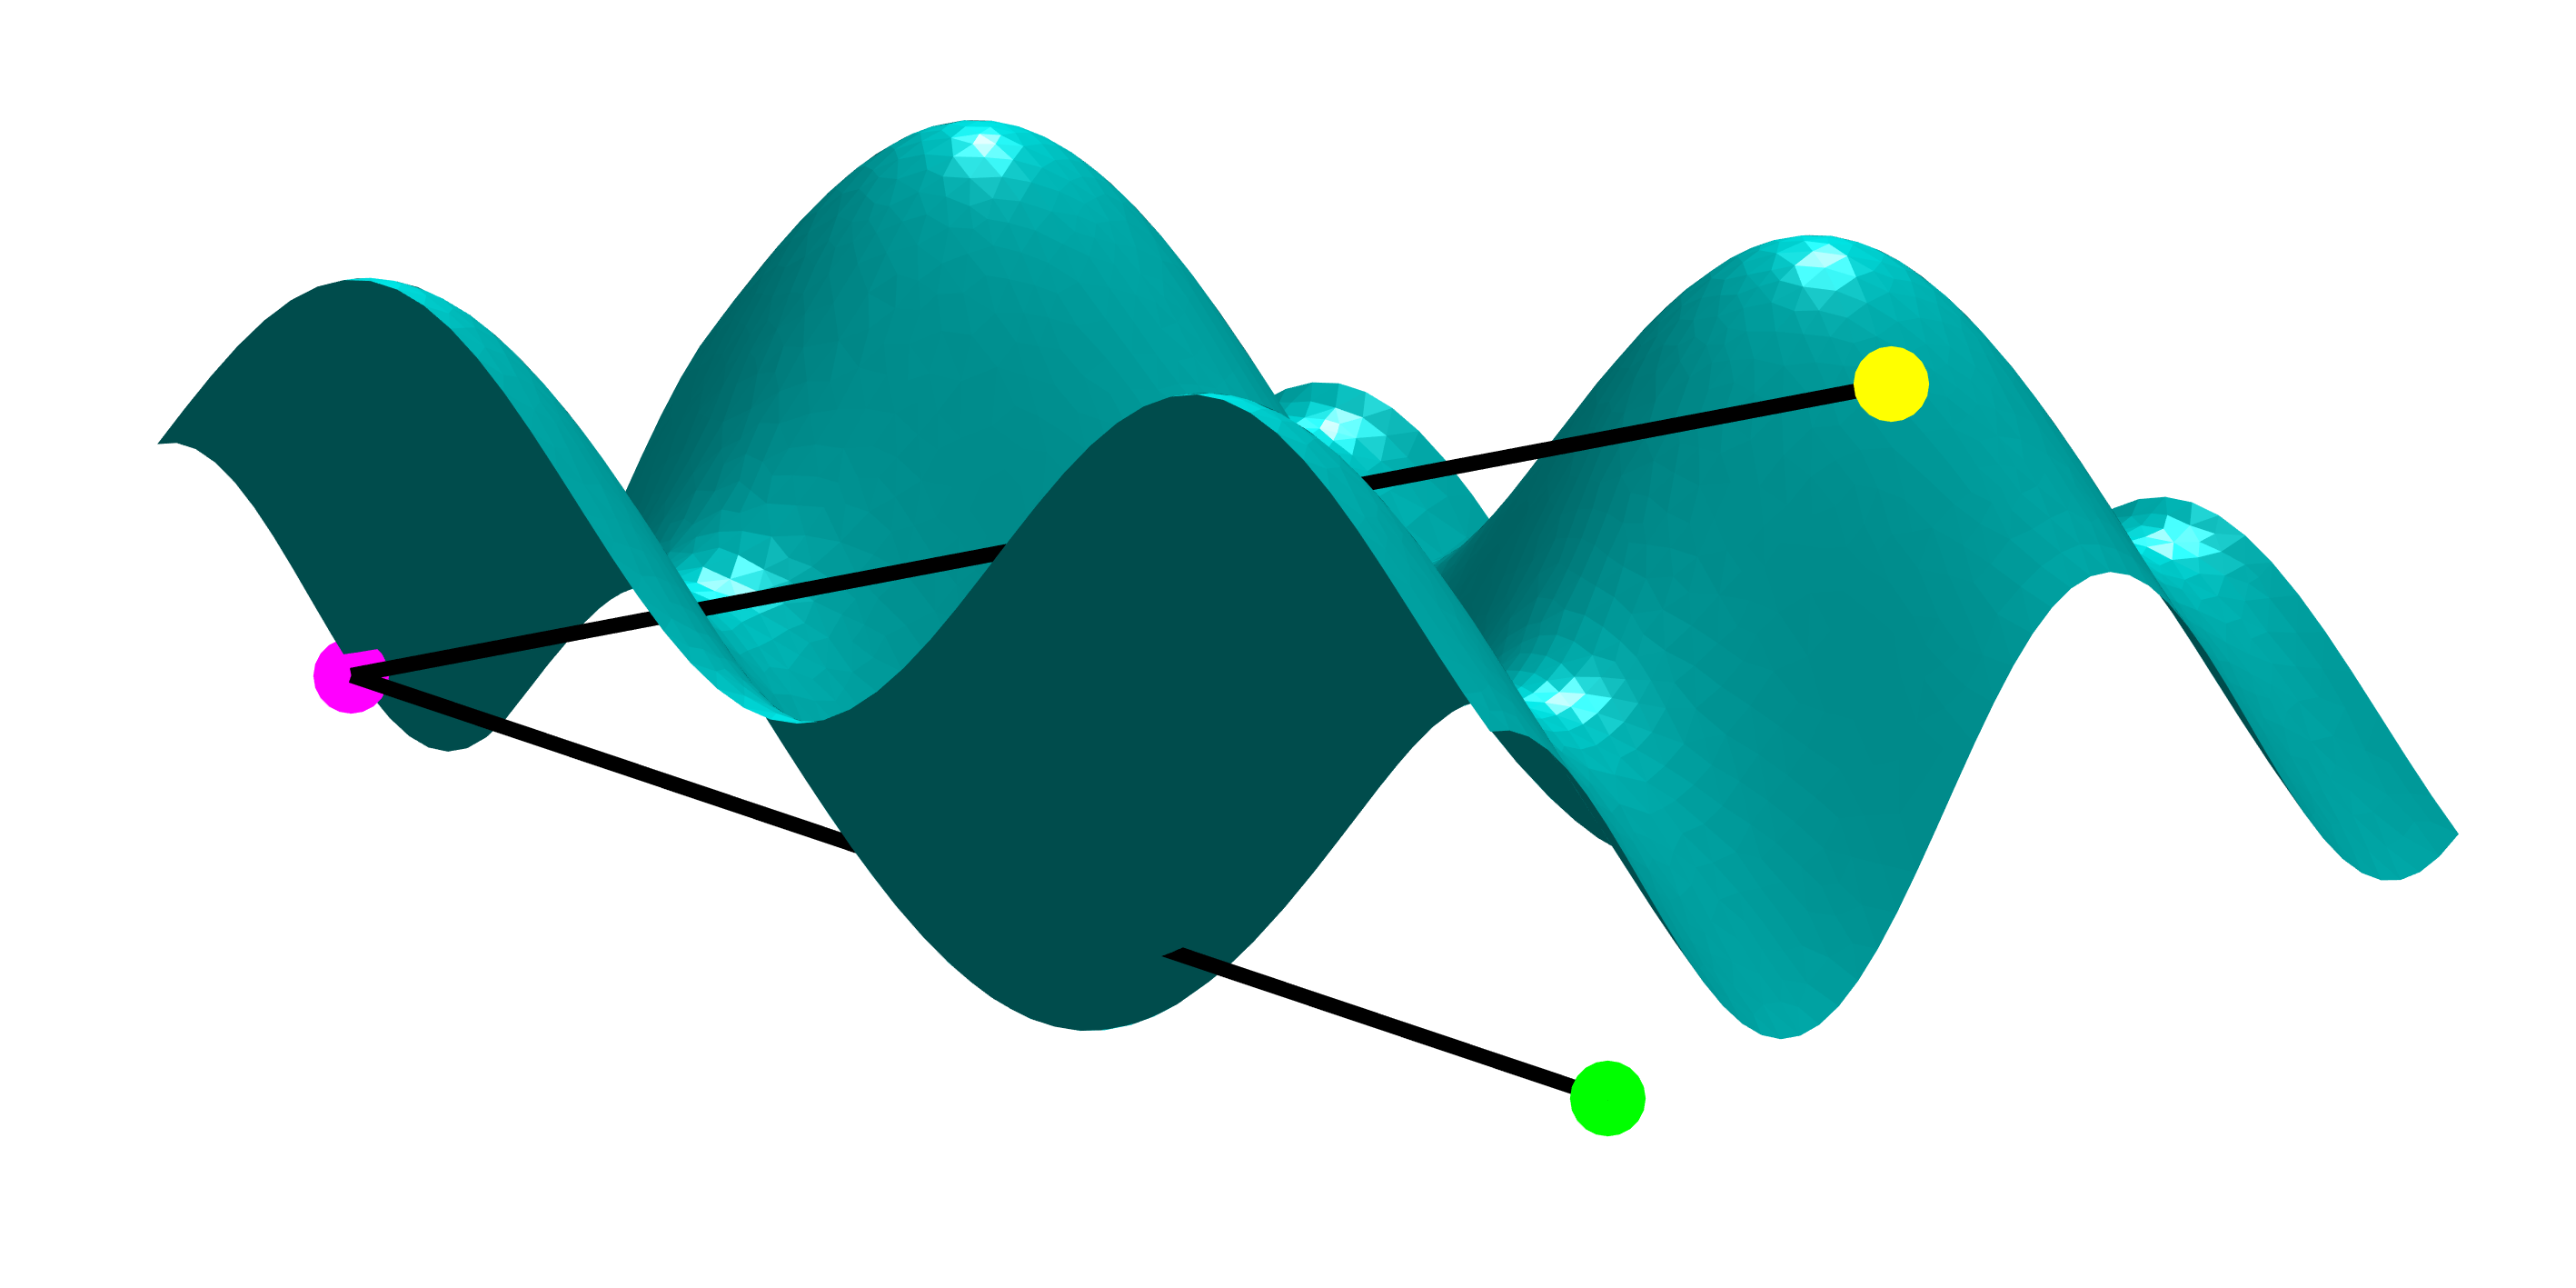
\includegraphics[width = 0.8\textwidth]{raytest.png}
\caption{Reduced ray intersection test for non-contiguous surfaces. The root point (interior) is shown in magenta. A ray from an interior point (green) makes two intersections due to the presence of a fold; from an exterior point (yellow) there is one intersection.}
\label{raytest}
\end{figure}

In order to minimise the number of tests required per voxel, convex hulls (defined as the smallest possible region enclosing a set of points within which any two points can be connected without leaving the region \cite{DeBerg2008}) are used to estimate partial volumes wherever possible. The rationale for this is that if the extrema points of a region can be classified as interior/exterior to a surface then, to an approximation, all points lying within the convex hull of these points will share the same classification. 

\section{Algorithmic implementation}

The following section addresses PV estimation for structures within the brain, for which the tissue classes of interest are GM, WM and non-brain. The same principles would apply to structures in other areas of the body, though the interpretation of tissue classes would differ. 

\subsection{Estimation for a single surface}

The core algorithm within Toblerone estimates the voxel-wise interior/exterior PVs arising from the intersection of a single surface with an arbitrary voxel grid. Toblerone assumes cuboid voxels with a ‘boxcar’ (PSF), which is to say that it does not allow for any mixing of signal between voxels. In reality, different modalities have differing PSFs and such effects may be separately accounted for via a modality-specific convolution operation. 

\begin{figure}
\centering
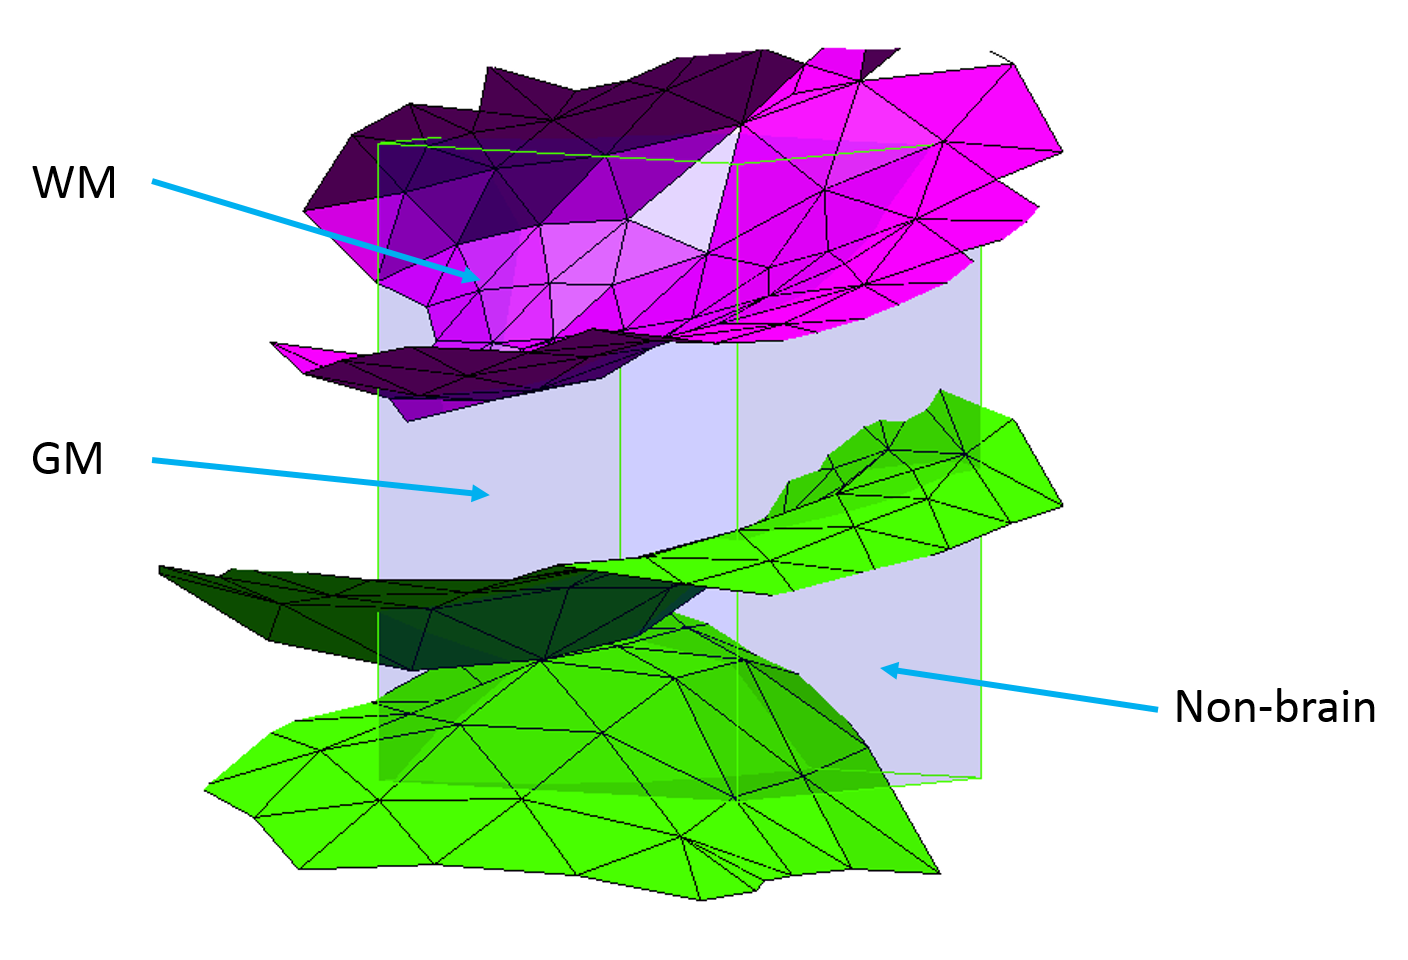
\includegraphics[width = 0.7\textwidth]{example_voxel.png}
\caption{Intersection of inner (magenta) and outer (green) surfaces of the cortex with a voxel. The outer surface intersects twice with distinct patches of surface; this is likely due to the presence of a sulcus. Tissue PVs are labelled.  }
\label{example_voxel}
\end{figure}

The first step is to identify and record the local patches of surface intersecting each voxel of the reference grid via Moller’s triangle-box overlap test \cite{Akenine-Moller2001}. The geometry of a surface within a voxel can frequently be complex: using a sulcus of the cortex as an example, the surface may intersect the voxel multiple times, with the opposite banks of the sulcus appearing as two unconnected patches of surface, illustrated in figure \ref{example_voxel}f. Accounting for the many possible surface/voxel configurations requires numerous specific tests that rapidly become excessively complex, so the approach taken in Toblerone is to divide and conquer each voxel as required. As the length scale of a voxel decreases, the complexity of the local surface configuration within the voxel will also decrease (for example, a sulcus is less likely to intersect the voxel multiple times). Each voxel of the reference image is therefore divided into a number of subvoxels which are processed individually. The subdivision factor has been set empirically as $\mathrm{ceil}(\vec{v} / 0.75)$ where $\vec{v}$ is the vector of voxel dimensions and 0.75 represents the lower limit of feature size found in the brain (in other contexts this parameter could be varied). Note that this subdivision factor transforms anisotropic voxels into approximately isotropic subvoxels,  which are processed according to the following framework. 

\begin{itemize}
\item If the subvoxel does not intersect the surface, it is assigned a single-class volume according to an interior/exterior classification of its centre. This is illustrated in figure \ref{all_subvoxels}a. 

\item If the subvoxel intersects the surface, then it contains interior and exterior PVs. One of these will be estimated using a convex hull (via the Qhull implementation \cite{Barber:1996:QAC:235815.235821}) if the geometry of the surface is favourable, as follows:

\begin{itemize}
\item If the surface intersects entirely through one face of the subvoxel, then it encloses a highly convex volume that may be reliably estimated. The other partial volume is calculated by subtraction from the total subvoxel volume. This is illustrated in figure \ref{all_subvoxels}b. 
\item If the surface is folded within the subvoxel (identified by multiple intersection of the surface along an edge or face diagonal of the subvoxel) then the subvoxel is subdivided a second time. This is because it is difficult to reliably identify which volume is interior or exterior in such a situation. This is illustrated in figure \ref{all_subvoxels}c/d. 
\item In all other cases, convex hulls are again used. In order to minimise the potential error associated with estimation of a non-convex volume via the use of a convex hull, it is important to identify which of the two PVs within the subvoxel is closer to being genuinely convex than the other. The proxy measure used for this is the number of subvoxel vertices lying on either side of the surface: the side with fewer vertices is assumed to enclose a more convex (and at any rate smaller) volume than the other. This is illustrated in figure \ref{all_subvoxels}e.
\end{itemize}

\item If the surface intersects the subvoxel multiple times (identified by the successful separation of surface vertices lying within the subvoxel into unconnected groups) then the voxel is subdivided a second time. This situation occurs for example when the opposite banks of a sulcus pass through a voxel. Although the reduced ray intersection test is accurate in such a situation, forming convex hulls is not, so subdivision is the safer option. This is illustrated in figure \ref{all_subvoxels}f. 
\end{itemize}

\begin{figure}
\centering
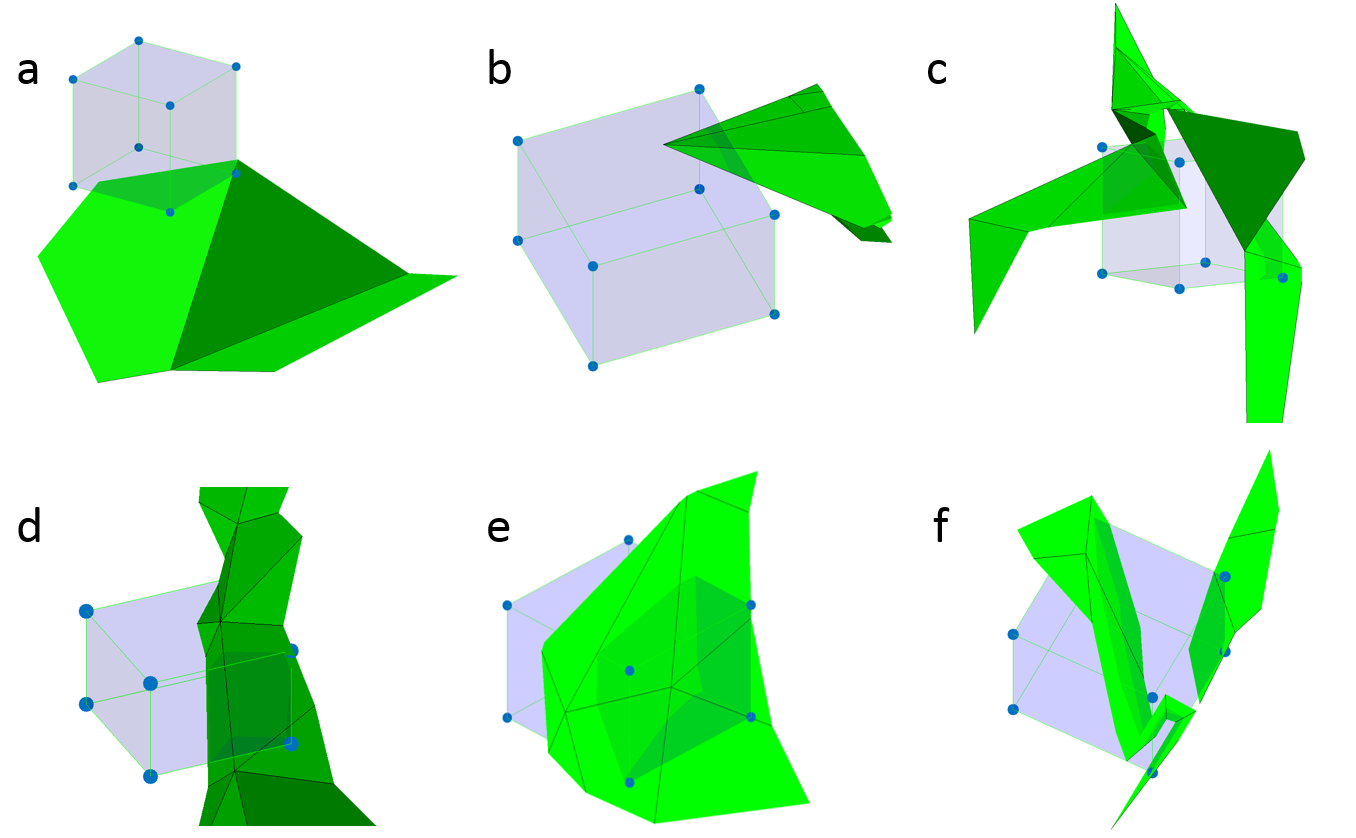
\includegraphics[width = \textwidth]{all_subvoxels.png}
\caption{Various subvoxel/surface configurations. a) no intersection: whole-volume assignment; b) single intersection through one face: a small convex hull will be formed; c/d) two examples of single intersection, folded surface: further subdivision will be used; e) single intersection through multiple faces: a convex hull will be formed; f) multiple surface intersection (unconnected patches of surface, likely a sulcus): further subdivision will be used. }
\label{all_subvoxels}
\end{figure}

If required, the second subdivision is performed at a constant factor of five to yield sub-subvoxels of approximately 0.1 to 0.2mm side length isotropic. These are always assigned a single-class volume based on a classification of their centre points as their small size means that any PVE will be negligible. Finally, voxels that do not intersect the surface (fully interior or exterior) are given single-class volumes according to tests of their centre points. Structures defined by a single surface (e.g. the thalamus) require no further processing: the estimates produced by the aforementioned steps may be used directly for PVEc.

\subsection{Estimation for multiple-surface structures}
Structures that are defined by multiple surfaces require further processing to yield PV estimates for all tissues of interest. Using the cortex as an example, PVs within each hemisphere are obtained with the following relations:

\begin{align}
PV_{WM} &= P_{inner} \\
PV_{GM} &= \mathrm{max}(0, P_{outer} - P_{inner}) \\
PV_{NB} &= 1 - (PV_{WM} + PV_{GM}) 
\end{align}

where $P_{inner}$ and $P_{outer}$ denote the interior/exterior PV fractions associated with the inner and outer surfaces of the cortex respectively and $PV_{WM}, PV_{GM}$ and $PV_{NB}$ denote the PV estimates for WM, GM and non-brain tissue (the latter including cerebrospinal fluid, CSF). These equations are structured to account for a potential surface defect whereby the surfaces of the cortex swap relative position (the inner lying exterior to the outer) around the corpus collosum. The structure of the above relations ($N$ surfaces leading to $N+1$ tissue classes) could easily be generalised to structures defined by more than two surfaces (for example, sublayers of the cortex, as used in laminar fMRI). A similar set of equations is used to merge hemisphere-specific results to cover the whole cortex, accounting for voxels lying on the mid-sagittal plane that intersect both hemispheres.

\subsection{Whole-brain PV estimation}
Toblerone, as outlined above, operates on a structure-by-structure basis in which the output tissue types are dependent on the structure in question. A number of methods utilising this core functionality have been implemented for general use cases: 
\begin{itemize}
	\item \textit{estimate\_structure}: estimate the interior and exterior PVs associated with a structure defined by a single surface
	\item \textit{estimate\_cortex}: estimate the GM, WM and non-brain PVs associated with the four surfaces of the cortex (l/r white/pial in the FreeSurfer terminology) 
	\item \textit{estimate\_all}: a combination of the structure and cortex methods above, this estimates PVs for the cortex and all subcortical structures identified by FIRST and combines them (with the exception of the brain stem) into a single set of GM, WM and non-brain PV estimates. 
\end{itemize}
The run-time for \textit{estimate\_all} running on the output of FreeSurfer and FSL FIRST for a single subject was around 20 minutes on a desktop machine; given the vector-heavy nature of the calculations involved, this could likely be reduced on GPU hardware. 

The combination of FreeSurfer/FIRST and Toblerone's \textit{estimate\_all} provides a complete pipeline for obtaining whole-brain PV estimates in an arbitrary reference voxel grid from a single T1-weighted image that may be used as a replacement for existing volumetric PV estimation tools such as FAST. There is however a key conceptual difference between surface and volumetric methods that concerns their interpretation of subcortical structures. Due to differences in tissue composition around the brain, cortical and subcortical GM typically have different intensities on a normal T1-weighted image (whereby cortical GM is seen as more ‘grey’ than subcortical, as illustrated in figure \ref{subcortical_gm_differences}). Being a histogram-based method, FAST will generally assign subcortical GM a lower GM PV estimate than might be expected as a result. In fact, by default FAST does not use any structural prior information and so is not even aware that these two different types of GM are in the same `class'; it simply determines subcortical GM to be more similar to cortical GM than it is to WM. 

Surface-based methods, by contrast, cannot take a nuanced view of the tissue composition of a subcortical structure. The surface that is used as input is treated as an absolute truth, with the implication that whatever tissue lies inside it is of a single type and is different to that outside. As a result, the tissue type of a structure must be determined using contextual or prior information (a conventional volumetric segmentation may be used to determine which tissue lies outside a structure). Thus, when combining the PVs of individual structures in Toblerone’s \textit{estimate\_all} function, it is necessary to know \textit{in advance} how the tissue type of each structure should be interpreted. In this work, all subcortical structures identified by FIRST (with the exception of the brain stem) were treated as pure GM. The practical implication of this is that Toblerone’s estimates for subcortical GM are higher than those produced by FAST (illustrated in figure \ref{subcortical_gm_differences}). For this reason, the conventional GM/WM/CSF tissue classes used by volumetric tools may be better thought of within Toblerone’s framework as tissue of interest, other tissues and non-brain, though for the purposes of this article the familiar names GM and WM shall be used alongside non-brain. The inherent ambiguity in determining which tissues lie outside subcortical structures, which could be either WM or CSF depending on their location within the brain, was resolved using FAST’s segmentation results.

\begin{figure}[H]
\centering
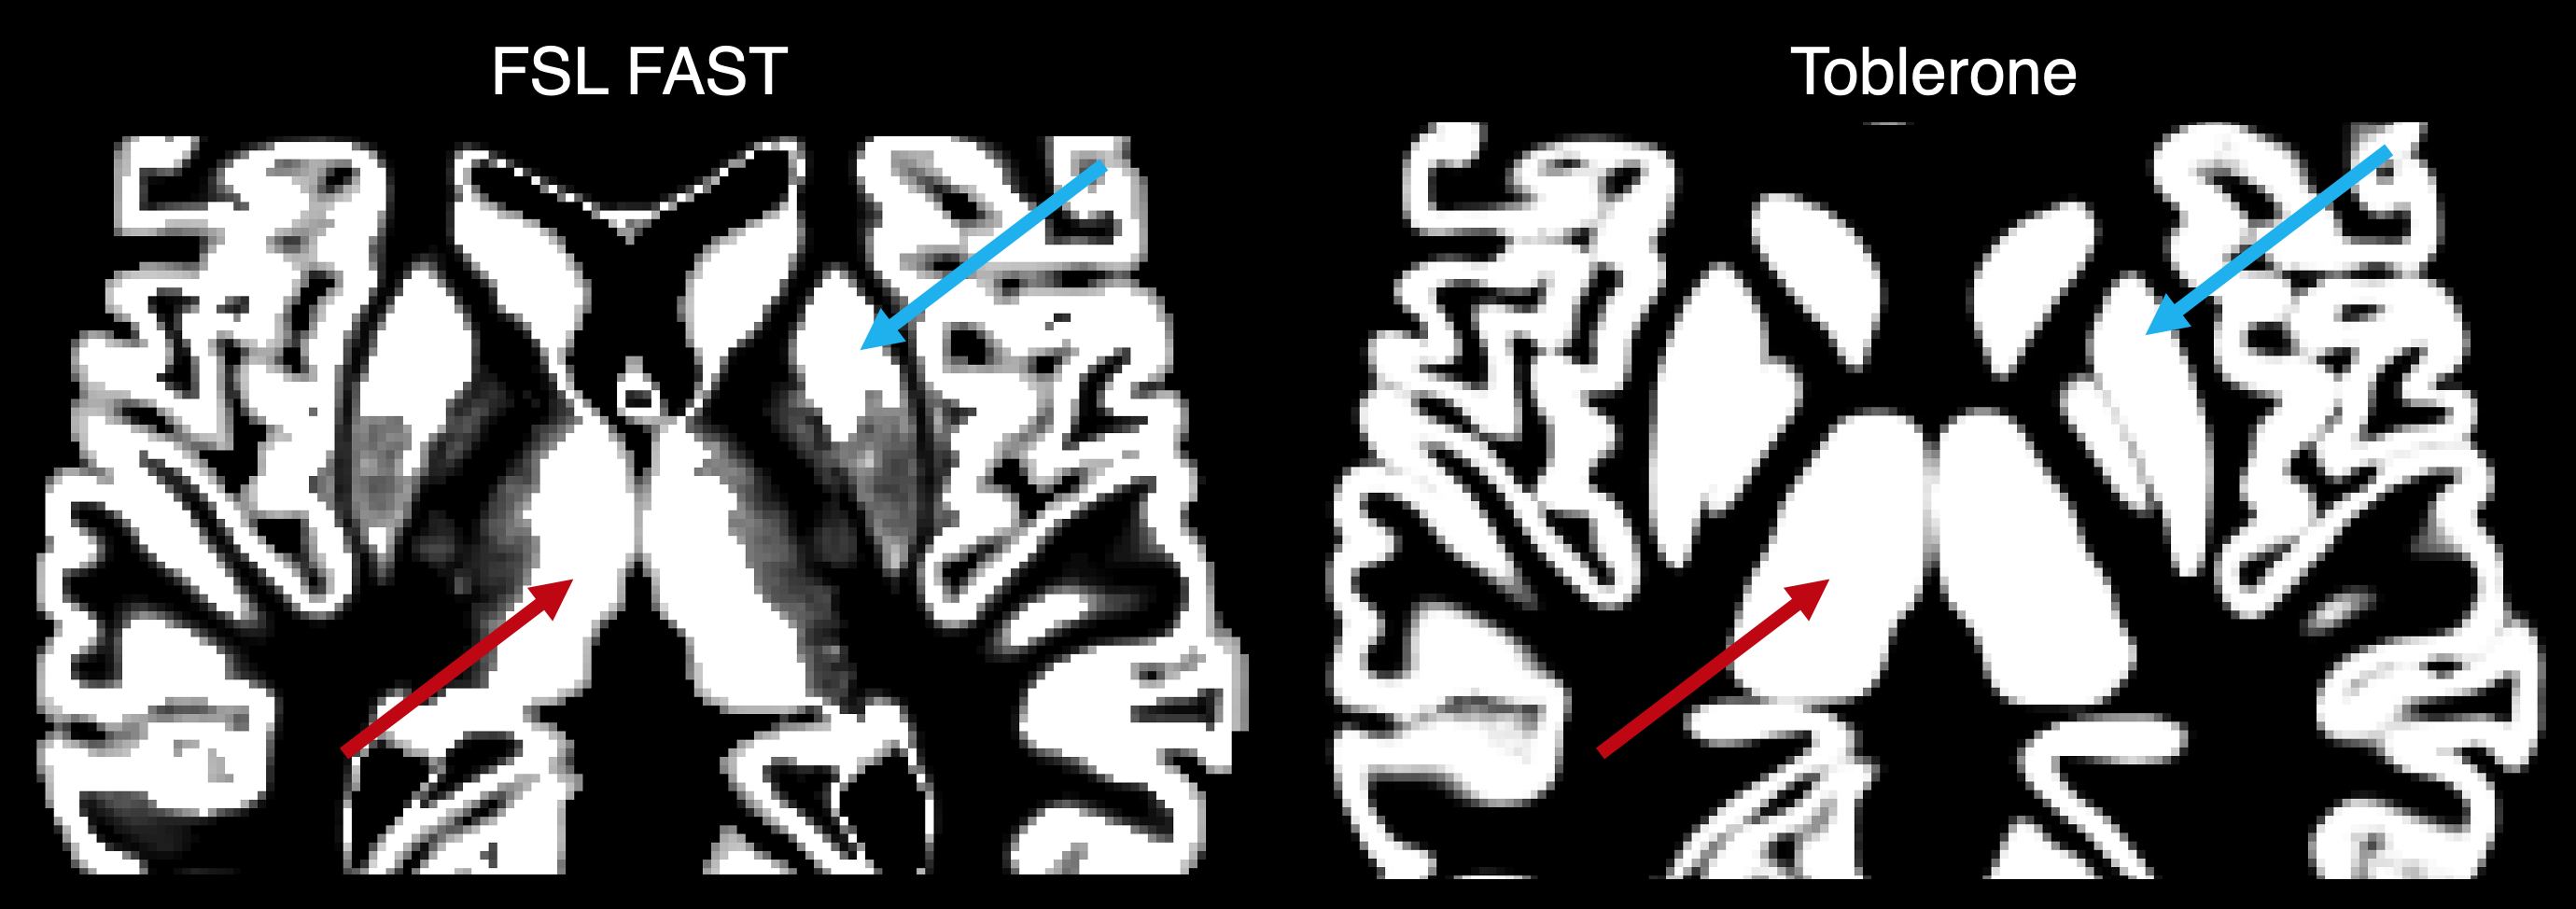
\includegraphics[width = \textwidth]{subcortical_gm_differences.png}
\caption{The left thalamus (red) and right putamen (blue) highlighted on the GM PV estimates of Toblerone and FAST on a typical subject, showing how surface and volumetric methods differ markedly in their interpretation of subcortical structures (FAST does not regard them as pure GM, whereas Toblerone does for the analyses presented in this work).}
\label{subcortical_gm_differences}
\end{figure}

\section{Methods}

\label{tob_pv_evaluation}

Three comparator methods were used to evaluate Toblerone. The two surface-based comparator methods were restricted to use in the cortex only as they cannot operate on subcortical structures defined by a single surface. Toblerone was run on both cortical and subcortical surfaces where possible to produce whole-brain PV estimates. 

The first surface-based comparator method, the ribbon-constrained (RC) algorithm, was developed for use with BOLD data in the HCP’s \textit{fMRISurface} pipeline \cite{Glasser2013} and is restricted to use in the cortex only. The method assumes vertex correspondence between the two surfaces of the cortex and works as follows. For each vertex in turn, the outermost edges of the triangles that surround that vertex are connected between the two surfaces to form a 3D polyhedron representing a small region of cortex. Nearby voxels are subdivided and the subvoxels centres tested to determine if they lie interior to the polyhedron. The subdivision factor used in this work was the higher value of either $\mathrm{ceil}( \mathrm{max} (\vec{v}/0.4) )$ or 4, where v is the vector of voxel dimensions. The fraction of subvoxel centres lying within any cortical polyhedron gives the cortical GM PV, which, as the BOLD signal is predominantly cortical in origin, is the quantity of interest for this modality. In order to obtain WM and non-brain PVs, the following post-processing steps were used. Firstly, the unassigned PV of each voxel was calculated as $1-PV_{GM}$, which was subsequently labelled as either WM or non-brain according to a signed-distance test of the voxel centre in comparison to the cortical mid-surface: for a voxel with centre point outside the mid-surface, the unassigned PV was labelled as non-brain. A weakness of this approach is that it is unable to faithfully capture a voxel in which all \textit{three} tissues are present; only the combinations WM/GM or GM/non-brain are permitted. As voxel size increases, the probability of voxels containing multiple tissues also increases; testing on an image of 3mm isotropic resolution showed that around 30\% of voxels intersecting the cortical ribbon contained three tissues. Resampling can be used to mitigate this effect so two variants of this method were tested: ‘RC’, direct estimation at each resolution, and ‘RC2’, estimation at 1mm followed by resampling to other resolutions via the process in section \ref{applywarp}. The run-time for a typical subject was around 15 minutes. 

\DIFdelbegin \DIFdel{This }\DIFdelend \DIFaddbegin \DIFadd{The }\DIFaddend second surface method, NeuroPVE \cite{NeuropolyPVE}, is based on the voxelisation work of \cite{Nooruddin2003}, applied in a brain-specific context and again restricted to use in the cortex only. Multiple expanded and contracted copies of each cortical surface are created and the ratio of expanded to contracted surfaces intersecting a given voxel is used as a first approximation for partial volumes. This ratio is then mapped, along with surface orientation information, via trigonometric relations on the unit cube into a PV estimate. The estimates produced take discrete values according to the number of surfaces used (in this work the default of five). The intended use of this tool was PV estimation at structural, not functional, resolution, so two variants were tested: ‘Neuro’, direct estimation at arbitrary resolutions, and ‘Neuro2’, estimation at structural resolution followed by resampling to other resolutions via the process in section \ref{applywarp}. On the basis of NeuroPVE’s results on the simulated surfaces, it was excluded from further analysis. As the process of surface inflation is slow, the run-time for a typical subject was around 12 hours. 

Finally, FSL’s FAST \cite{Zhang2001} is an established whole-brain volumetric segmentation tool that was used as a comparator for the surface methods. On both the BrainWeb and HCP test-retest datasets, FAST was run on the brain-extracted images at structural resolution (1mm and 0.7mm isotropic respectively). PVs were then obtained at other resolutions via the resampling method detailed in paragraph \ref{applywarp}. The run-time for a typical subject was around five minutes. 

\subsection*{Resampling via applywarp}
\label{applywarp}
Resampling is an interpolation operation that is used to transform volumetric data between voxel grids (in this context, from structural to functional resolution). FSL’s \textit{applywarp} tool was used with the \textit{-super} flag for all resampling operations. This works by creating an up-sampled copy of the target voxel grid onto which values from the input image are sampled. The average is then taken across the voxel neighbourhoods of the high-resolution grid (sized according to the up-sampling factor) to obtain the result in the target voxel grid. Such an approach is appropriate when moving from fine to coarse as each output voxel corresponds to multiple input voxels, the individual contributions of which should be accounted for to preserve overall tissue proportions. When using \textit{applywarp} a transformation matrix between the input and output voxel grids must be given as the \textit{-premat} argument; to denote identity for the purposes of this work, the output of the HCP \textit{wb\_command –convert-affine –from-world –to-flirt} tool operating on the identity matrix $\mat{I}_4$ was used as the \textit{-premat} to correct for a subvoxel shift that arises due to FSL coordinate system conventions. Note that for perfectly aligned voxel grids with an integer ratio of voxel sizes, such as a 1mm and 2mm isotropic grid, this process is equivalent to averaging across blocks of the smaller grid (sized 2x2x2 in this case).

\section{Datasets}

Four datasets were used to evaluate Toblerone. Three of these pertained to PV estimation specifically, as summarised in table \ref{tob_datasets}, and the final one investigated the link between PV estimates and PVE in physiological data.

\begin{table}[H]
\setlength{\tabcolsep}{0.75em} % for the horizontal padding
{
    \renewcommand{\arraystretch}{1.2}% for the vertical padding
    \begin{tabular}{p{2.5cm}|p{3.5cm}p{3.5cm}p{3.6cm}}
    \textit{name} & Simulated surfaces & BrainWeb & HCP test-retest \\ \cline{1-4}
    \textit{type} & S & V \& S & V \& S \\
    \textit{resolution} & - & 1mm iso. & 0.7mm iso. \\
    \textit{size} & \begin{tabular}[c]{@{}l@{}}one cortical \\hemisphere \end{tabular} & \begin{tabular}[c]{@{}l@{}}one subject, \\18 structural images\end{tabular} & \begin{tabular}[c]{@{}l@{}}45 subjects,\\2 structural images each\end{tabular} \\
    \textit{ground truth} & numerical method & volumetric segmentation* & N/A \\
    \textit{comparator methods} & \begin{tabular}[c]{@{}l@{}}NeuroPVE (S)\\ RC (S)\end{tabular} & \begin{tabular}[c]{@{}l@{}}RC** (S)\\ FAST (V)\end{tabular} & \begin{tabular}[c]{@{}l@{}}RC** (S)\\ FAST (V)\end{tabular}
    \end{tabular}
}
\caption{Overview of methods and datasets used for evaluation of PV estimation. Key: S: surface, V: volumetric, RC: ribbon-constrained. 
* established via automatic segmentation with manual intervention. ** RC can only operate on the cortex, not subcortex, for these datasets.}
\label{tob_datasets}
\end{table}

\subsection{Simulated surfaces}
\label{tob_sim_surfaces}
A pair of concentric surfaces, illustrated figure \ref{simsurfs}, were designed to capture geometric features relevant to the anatomy of a cortical hemisphere. These were produced by modulating the radius of a sphere as a function of azimuth $\theta$ and elevation $\phi$ to produce sulcal and gyral-like features. The radius of the inner surface was defined as

\begin{equation}
r_{in} = 60 (1 - 0.1 \mathrm{max}(\sin^{20}(5u), \sin^{20}(5v) ) )
\end{equation}

where 60 is the unmodulated radius of the sphere, 0.1 fixes the relative depth of sulci, the max function prevents sulci from constructively interfering to produce deep wells at points of intersection, the power of 20 produces broad gyri and narrow sulci, and the substitutions $u= \phi + \theta$, $v= \phi - \theta$ cause the sulci to spiral around the sphere in opposite directions. Modulation was restricted to the range $-2\pi/5 \leq \theta \leq 2\pi/5$ to leave the poles smooth and suppress unrealistic features. The outer radius was set at $r_{out}= 1.05 \cdot r_{in}$, leading to a peak radial distance between surfaces of 3mm. The outermost region was taken to represent non-brain tissue, the innermost WM and the region in between GM. The use of analytic functions to define the surfaces permitted ground truth to be calculated using the following numerical method. Voxels were sampled at 4,096 elements per mm\textsuperscript{3} and the positions of these sample points expressed in spherical polar coordinates. By comparing the actual radius of each point to the calculated radius of the surface boundaries for the same azimuth and elevation, the tissue type of the sample point within the structure could be determined, and from there PVs obtained by aggregating results within voxels. This is referred to as the ‘numerical solution’ in the results section. All surface methods were used on this dataset to obtain PVs at voxel sizes of 1 to 3mm in steps of 0.2mm isotropic. 

\begin{figure}
\centering
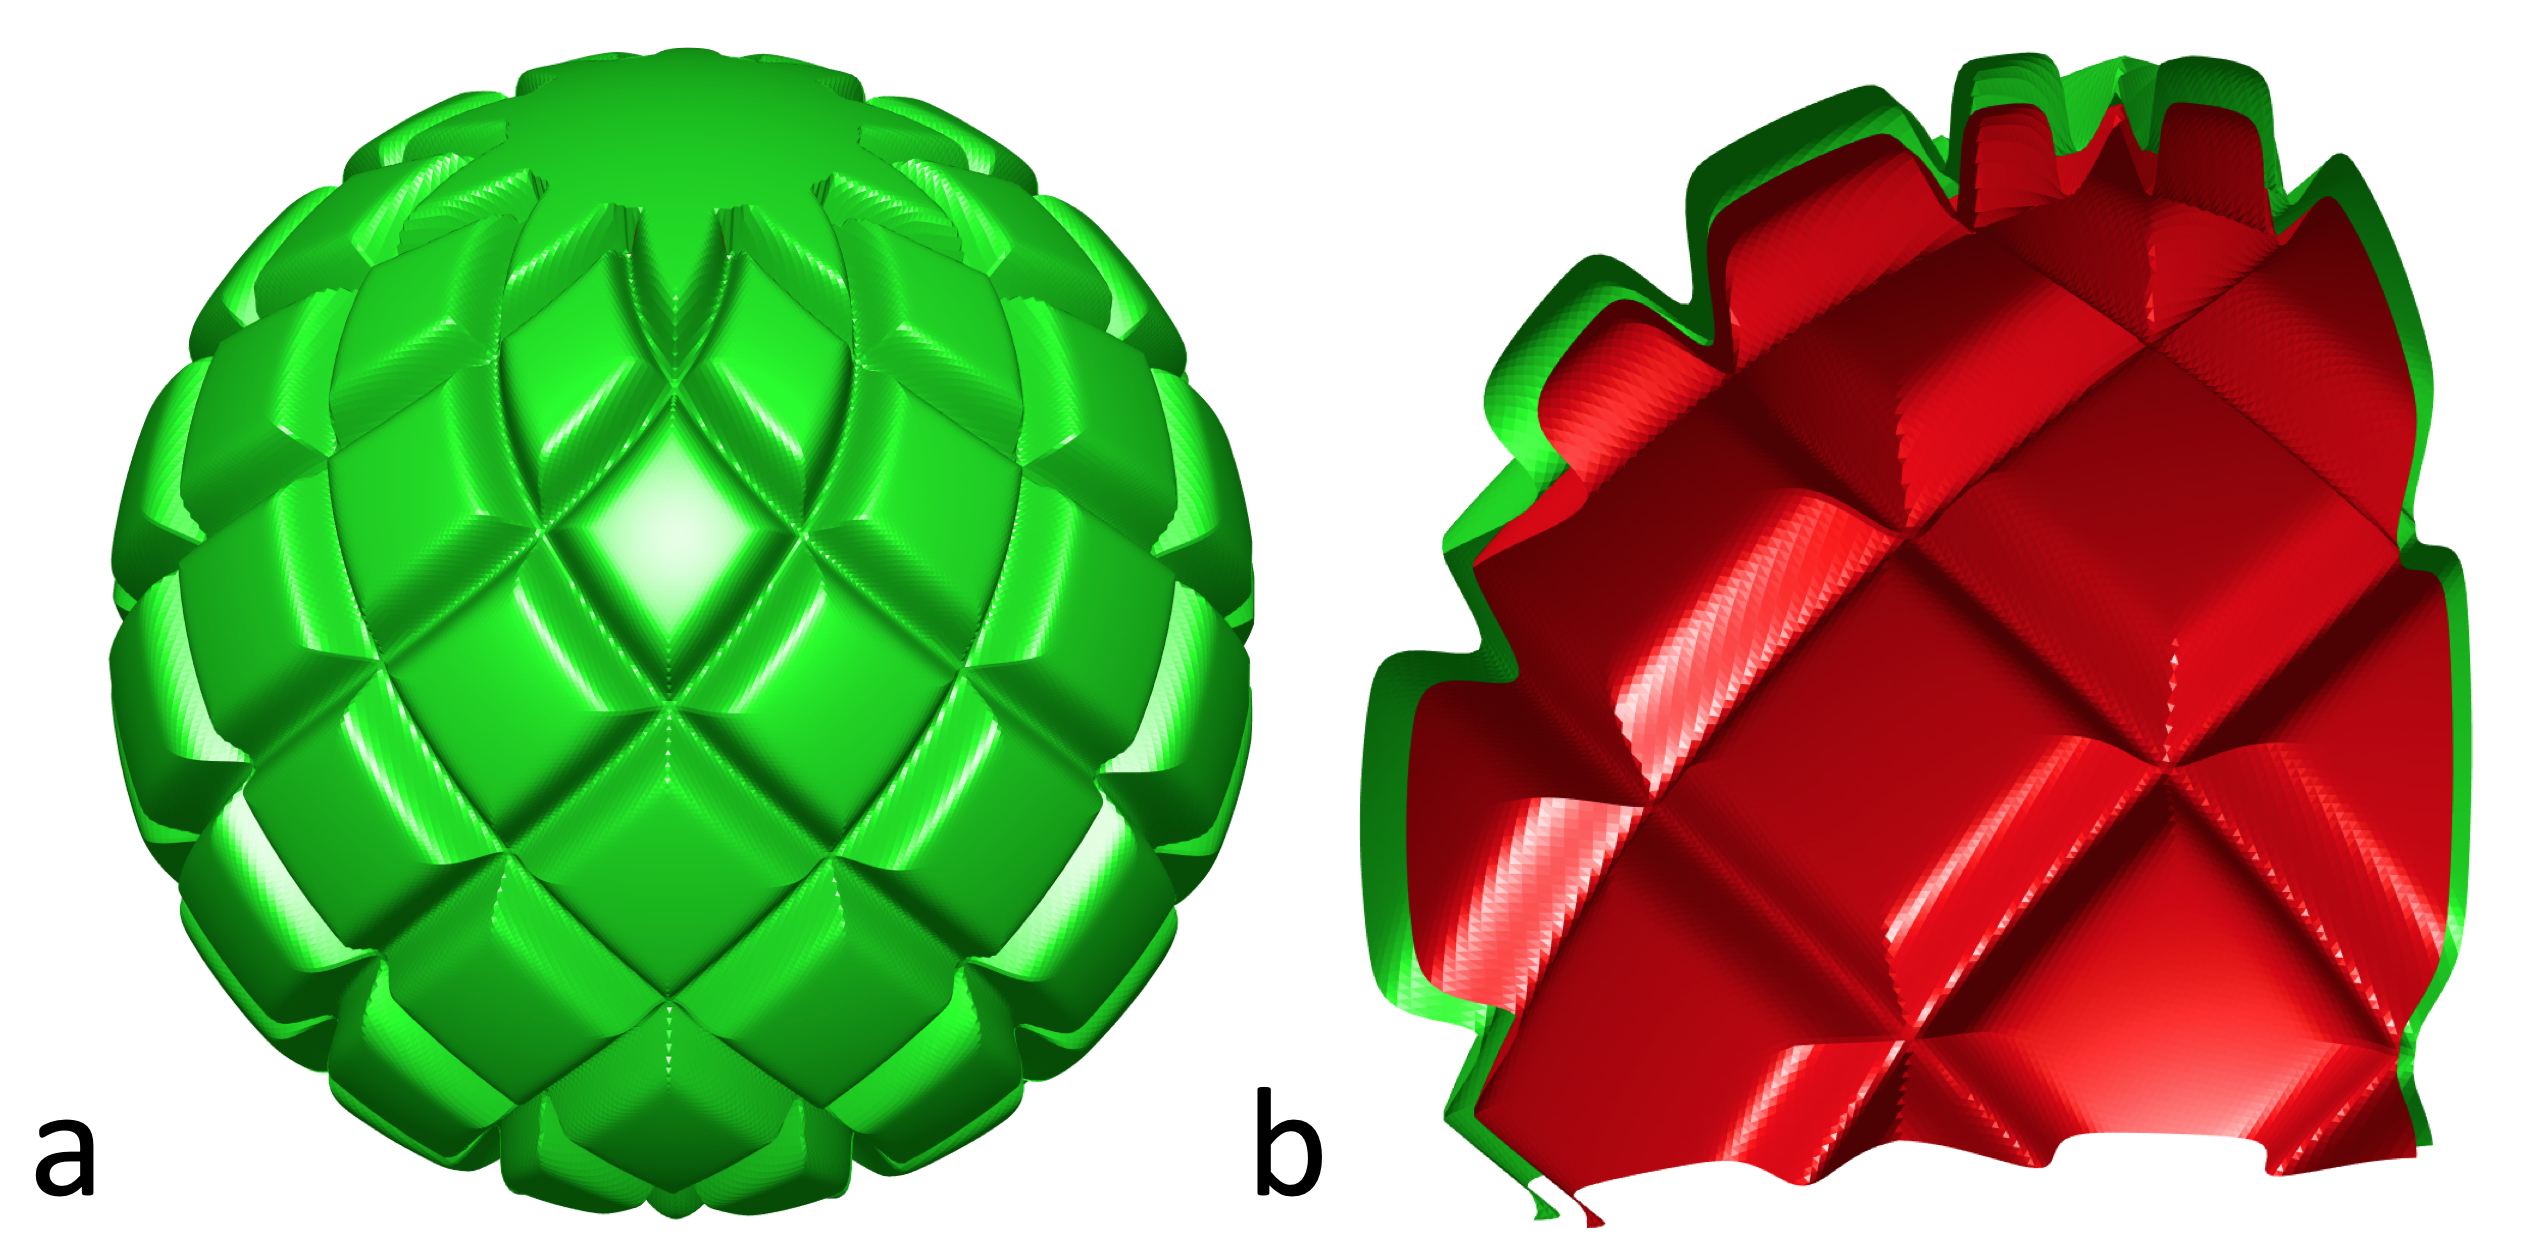
\includegraphics[width = 0.7\textwidth]{simsurfs.png}
\caption{a) Simulated surfaces; b) cutaway showing inner (red) and outer (green) surfaces. Peak radial distance between the two was 3mm.}
\label{simsurfs}
\end{figure}

\subsection{BrainWeb simulated T1 images}
BrainWeb \cite{Collins1998, Cocosco1997} simulates whole-head T1 images at 1mm isotropic resolution with specified levels of random noise and field non-uniformity (NU).  Eighteen images were produced to cover the available parameter space of noise levels 0, 1, 3, 5, 7, 9 and NU levels 0, 20, 40 (both quantities in percent). These were run through FIRST and FreeSurfer, after which Toblerone’s \textit{estimate\_all} and the RC method (cortex only) were used on the output. FAST was also used to enable a comparison between surface and volumetric methods. PVs were obtained at voxel sizes of 1 to 4mm in steps of 1mm isotropic. Although ground truth PV maps exist for this dataset (produced by automatic volumetric segmentation of T1 images with manual correction), both surface and volumetric methods returned significantly different results to these, raising the complicated question of determining which set of results is correct. In order to avoid making this judgement, each method was instead referenced to its own results on the ideal T1 image (0\% noise 0\% NU) in the 1mm isotropic voxel grid of the structural images; the objective of the test was to measure self-consistency across differing levels of noise and NU. The voxel grids associated with each voxel size were aligned such that results at 1mm could be used to calculate a reference at other sizes without resampling. 

\subsection{Human Connectome Project test-retest data} 
This dataset comprises 45 subjects from the main HCP cohort who underwent two separate structural scan sessions (mean age 30.2 years, mean time between sessions 4.8 months). Each session was processed using the pipeline in \cite{Glasser2013} to obtain cortical surfaces via FreeSurfer. Separately, the distortion-corrected T1 images were processed using FIRST to obtain subcortical surfaces. Toblerone’s \textit{estimate\_all} and the RC method (for the cortex only) were used on this dataset, as well as FAST for a comparison between surface and volumetric methods. PVs were obtained at voxel sizes of 1 to 3.8mm in steps of 0.4mm isotropic, as well as the native 0.7mm isotropic voxel grid of the structural images. As a ground truth is not defined for this dataset, each method’s results from the first session were used as a reference for the second session to permit self-consistency to be assessed. 

\subsection{\textit{In-vivo} ASL data} 
This dataset consists of ASL data at 1.5mm isotropic resolution from four subjects. For three subjects, four within-session repeats of 100 volumes were acquired; for the final subject a single repeat of 200 volumes was acquired. Other parameters were as follows: pASL FAIR QUIPSS-II at 7T field strength with a 2D EPI ascending readout, 32ms slice time, 1.8s TI, 700ms bolus duration and 0.95 inversion efficiency. \DIFaddbegin \DIFadd{Further details are given in appendix \ref{7T_appendix}. }\DIFaddend The data was downsampled without interpolation to 3mm isotropic resolution by summing across 2x2x2 voxel neighbourhoods to improve SNR and increase PVE. A T1w MP2RAGE structural image at 0.7mm isotropic resolution was obtained for each subject; these were processed to yield PV estimates from both the combined FreeSurfer/FIRST/Toblerone pipeline and FAST. CBF quantification was performed without PVEc using the \textit{oxford\_asl} pipeline \cite{Chappell2009, oxford-asl}; a T1 blood value of 2.2s \cite{Zhang2013} and voxel-wise calibration were used. The ASL data was analysed in native acquisition space; MCFLIRT and FLIRT \cite{flirt} were used to motion correct the data and register the T1w image to the ASL for the purpose of generating PV estimates in native space. \DIFaddbegin \DIFadd{EPI distortion correction was not performed, which would be expected to lead to areas of mis-alignment between the ASL data and the PV estimates; however due to the global nature of the analysis, the errors arising from this omission should be somewhat mitigated. The reader may refer back to figures \ref{ss_slices} and \ref{02_slices} to inspect the extent of distortion-induced misalignment. 
}\DIFaddend 

\subsection{Evaluation metrics}

For the PV estimation datasets, errors were measured in both a per-voxel (RMS of individual voxel errors) and aggregate (total tissue volume) sense. The former basis is important as PVEc is locally sensitive to the PV estimates \cite{Zhao2017a}; the latter basis reflects systematic bias at the aggregate level. All errors are expressed in percent and map directly to PV estimates without scaling: for example, a PV estimate of 0.5 against a reference value of 0.55 corresponds to an error of -0.05 or -5\%. Note that for some datasets where ground truth was not available, errors were measured with respect to each method's reference result (outlined earlier for each dataset). 

A further analysis of voxel-wise differences between Toblerone and FAST was performed on the HCP dataset at multiple voxel sizes by sorting voxels into 5\% width bins according to their Toblerone GM PV estimate. The difference (Toblerone – FAST) was calculated for each voxel and the mean taken across each bin. This quantity was then averaged across subjects and sessions (weighted to respect differences in brain volume).

For the \textit{in-vivo} ASL dataset only, linear regressions of non-PVEc CBF against GM PV were performed to assess the strength of the relationship between CBF and PV; theoretical understanding suggests this should be positive and approximately linear. Voxels containing at least 10\% GM PV on both Toblerone's and FAST's outputs were selected; using the intersection of both methods ensured that neither method was penalised in areas where they fundamentally disagreed about what tissues are present (notably, around some subcortical structures identified by FIRST). For the same reason, two separate regressions were performed: one with both cortical and subcortical GM, and the other considering the cortex only. The metric of interest in this analysis was the correlation coefficient ($R$ value); higher values imply that the PV estimates better explain the variation observed in the CBF data (which was known ahead of time to be corrupted by PVE). 

\section{Results}

\subsection{Simulated surfaces}

\begin{figure}[H]
\centering
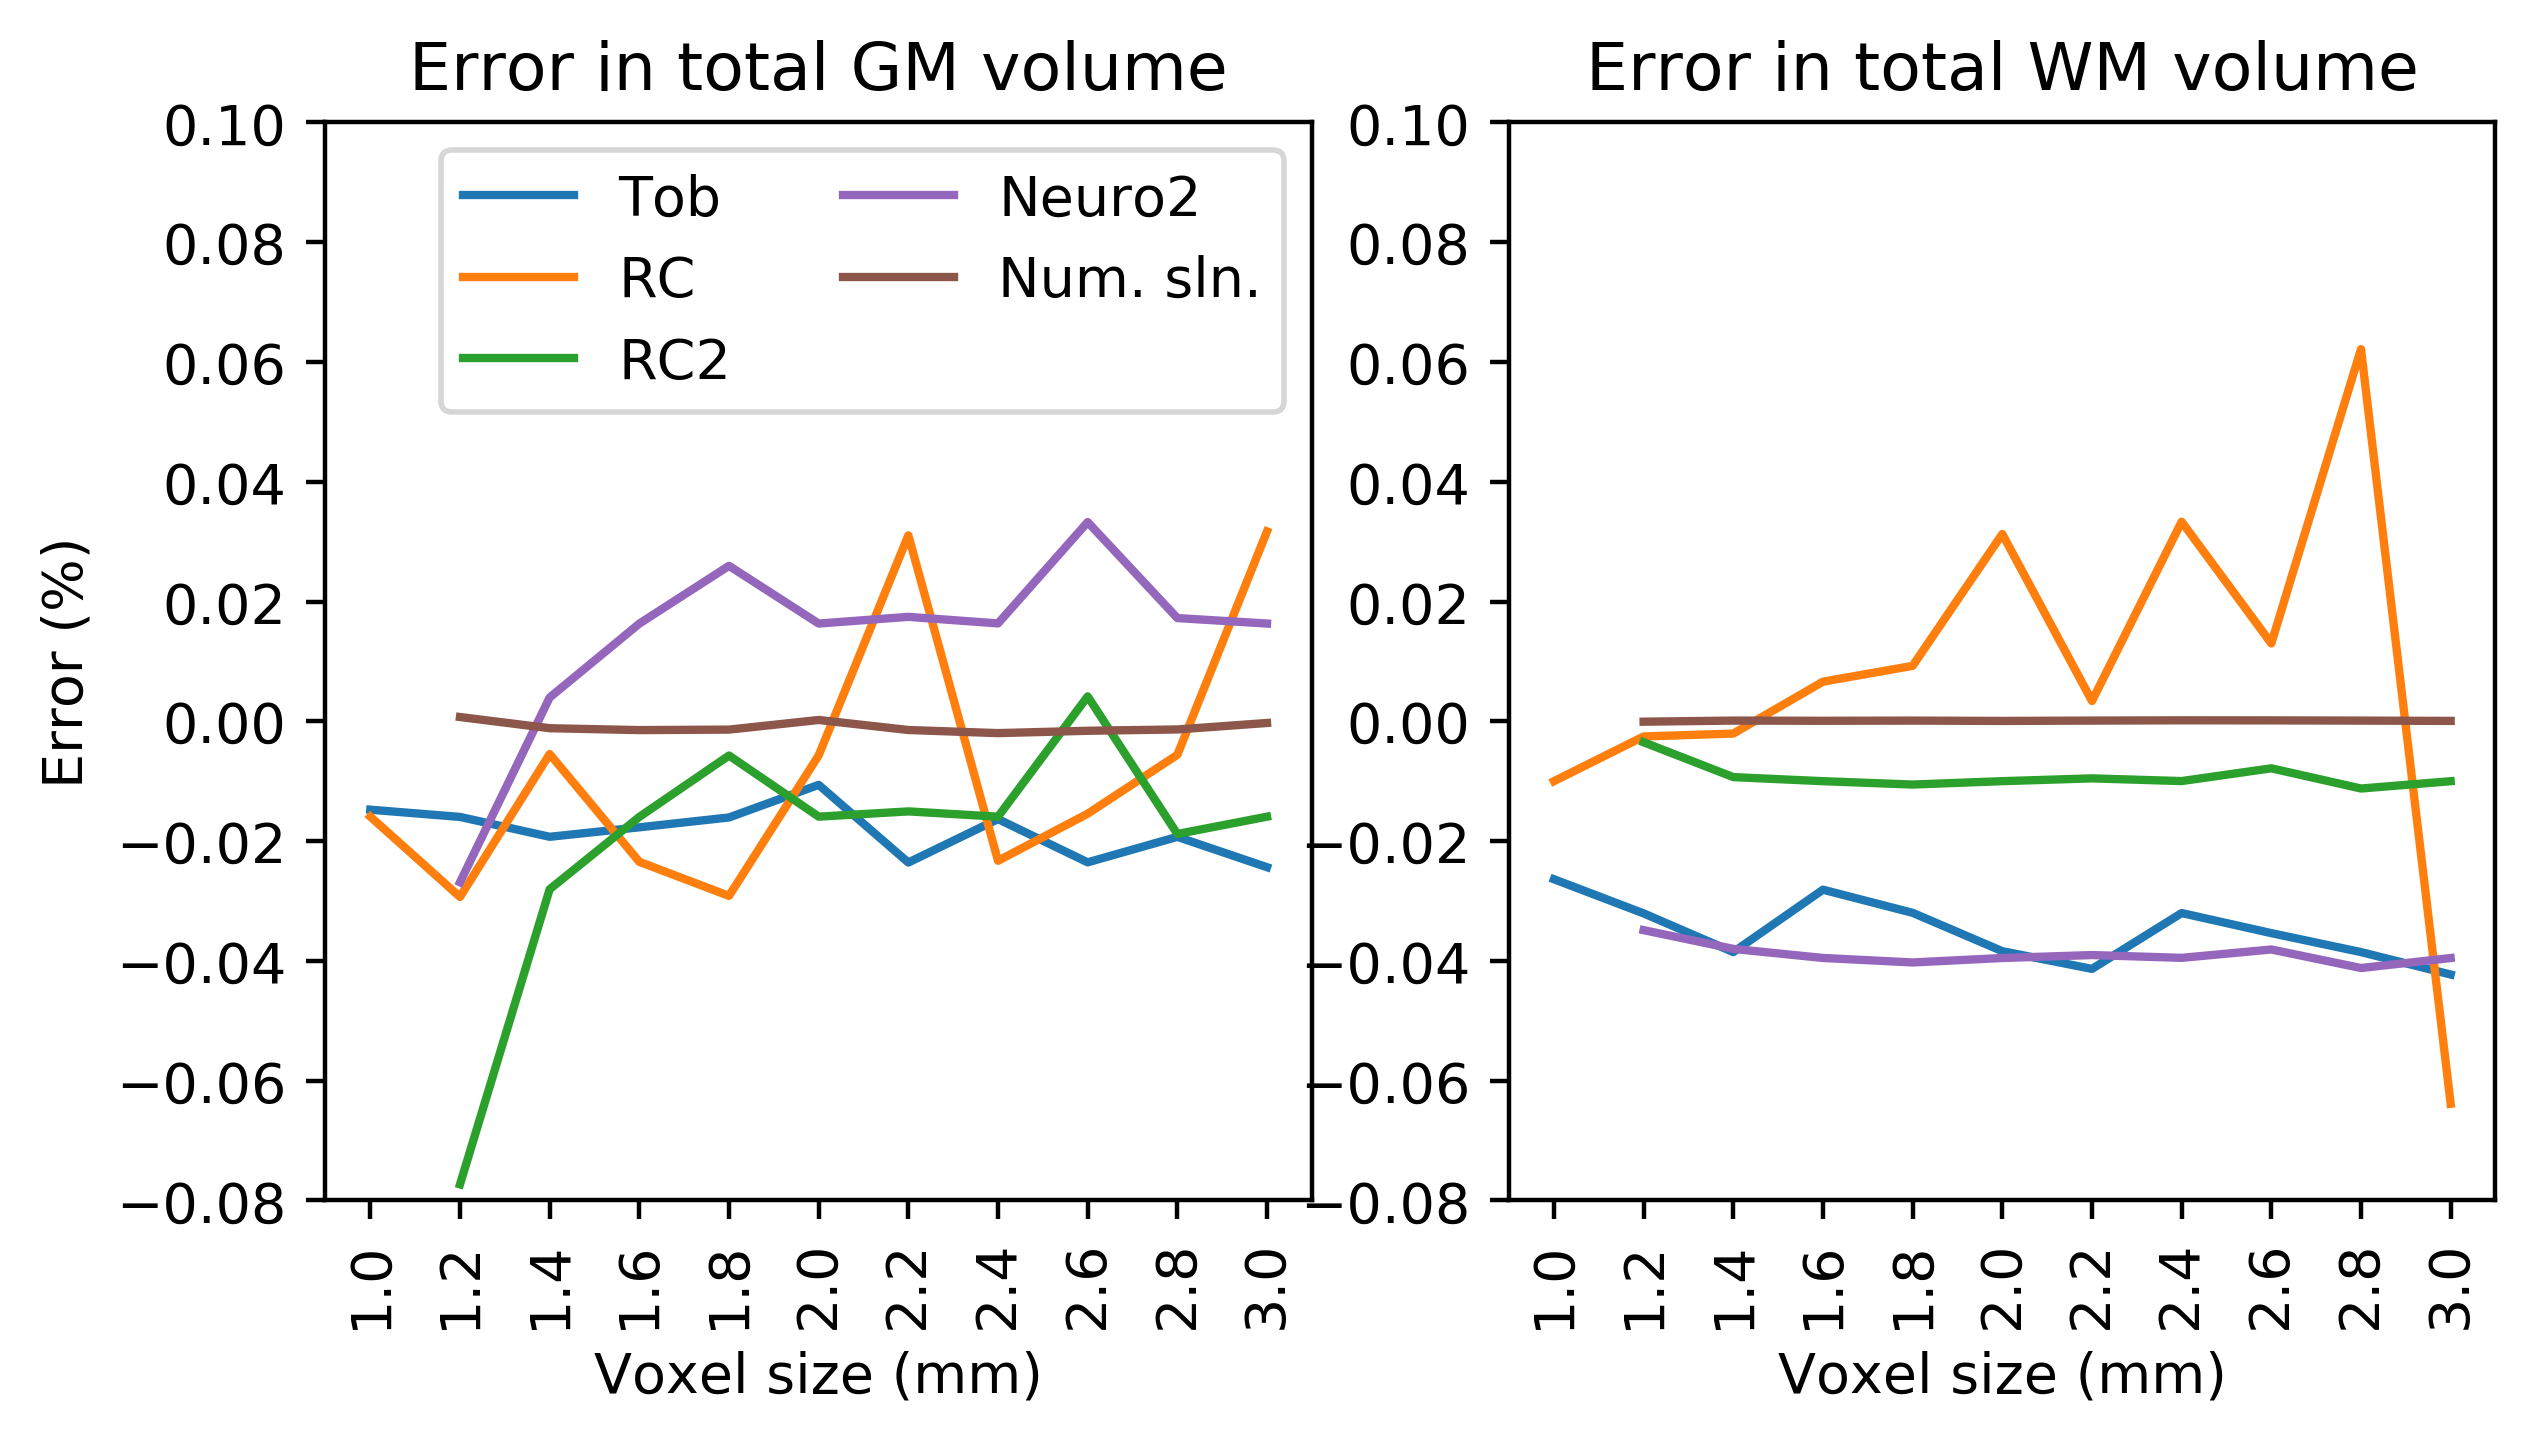
\includegraphics[width = 0.8\textwidth]{tob_sim_total.png}
\caption{Simulated surfaces: error in total tissue volume \DIFaddbeginFL \DIFaddFL{across all voxels, used to investigate bias and consistency across voxel sizes}\DIFaddendFL . Toblerone showed consistency, though with small bias, for both GM and WM. RC1 errors were lower for GM than WM. Resampling-based methods (RC2, Neuro2) showed particular consistency in WM. [Full results are in the appendix, figure \ref{tob_sim_total_supp}]}
\label{tob_sim_total}
\end{figure}

Figure \ref{tob_sim_total} shows the error in total tissue volume \DIFaddbegin \DIFadd{across all voxels }\DIFaddend for the simulated surfaces. The numerical solution at 1mm was used as the reference. Toblerone showed consistency across voxel sizes, though with a small negative bias in both GM and WM. RC estimates showed variation in both. The resampling-based methods RC2 and Neuro2 showed high consistency in WM but less so in GM. The numerical solution was stable across voxel sizes. Neuro’s results are excluded from this and subsequent graphs for clarity; the full results are given in the appendix, figure \ref{tob_sim_total_supp}). 

\begin{figure}[H]
\centering
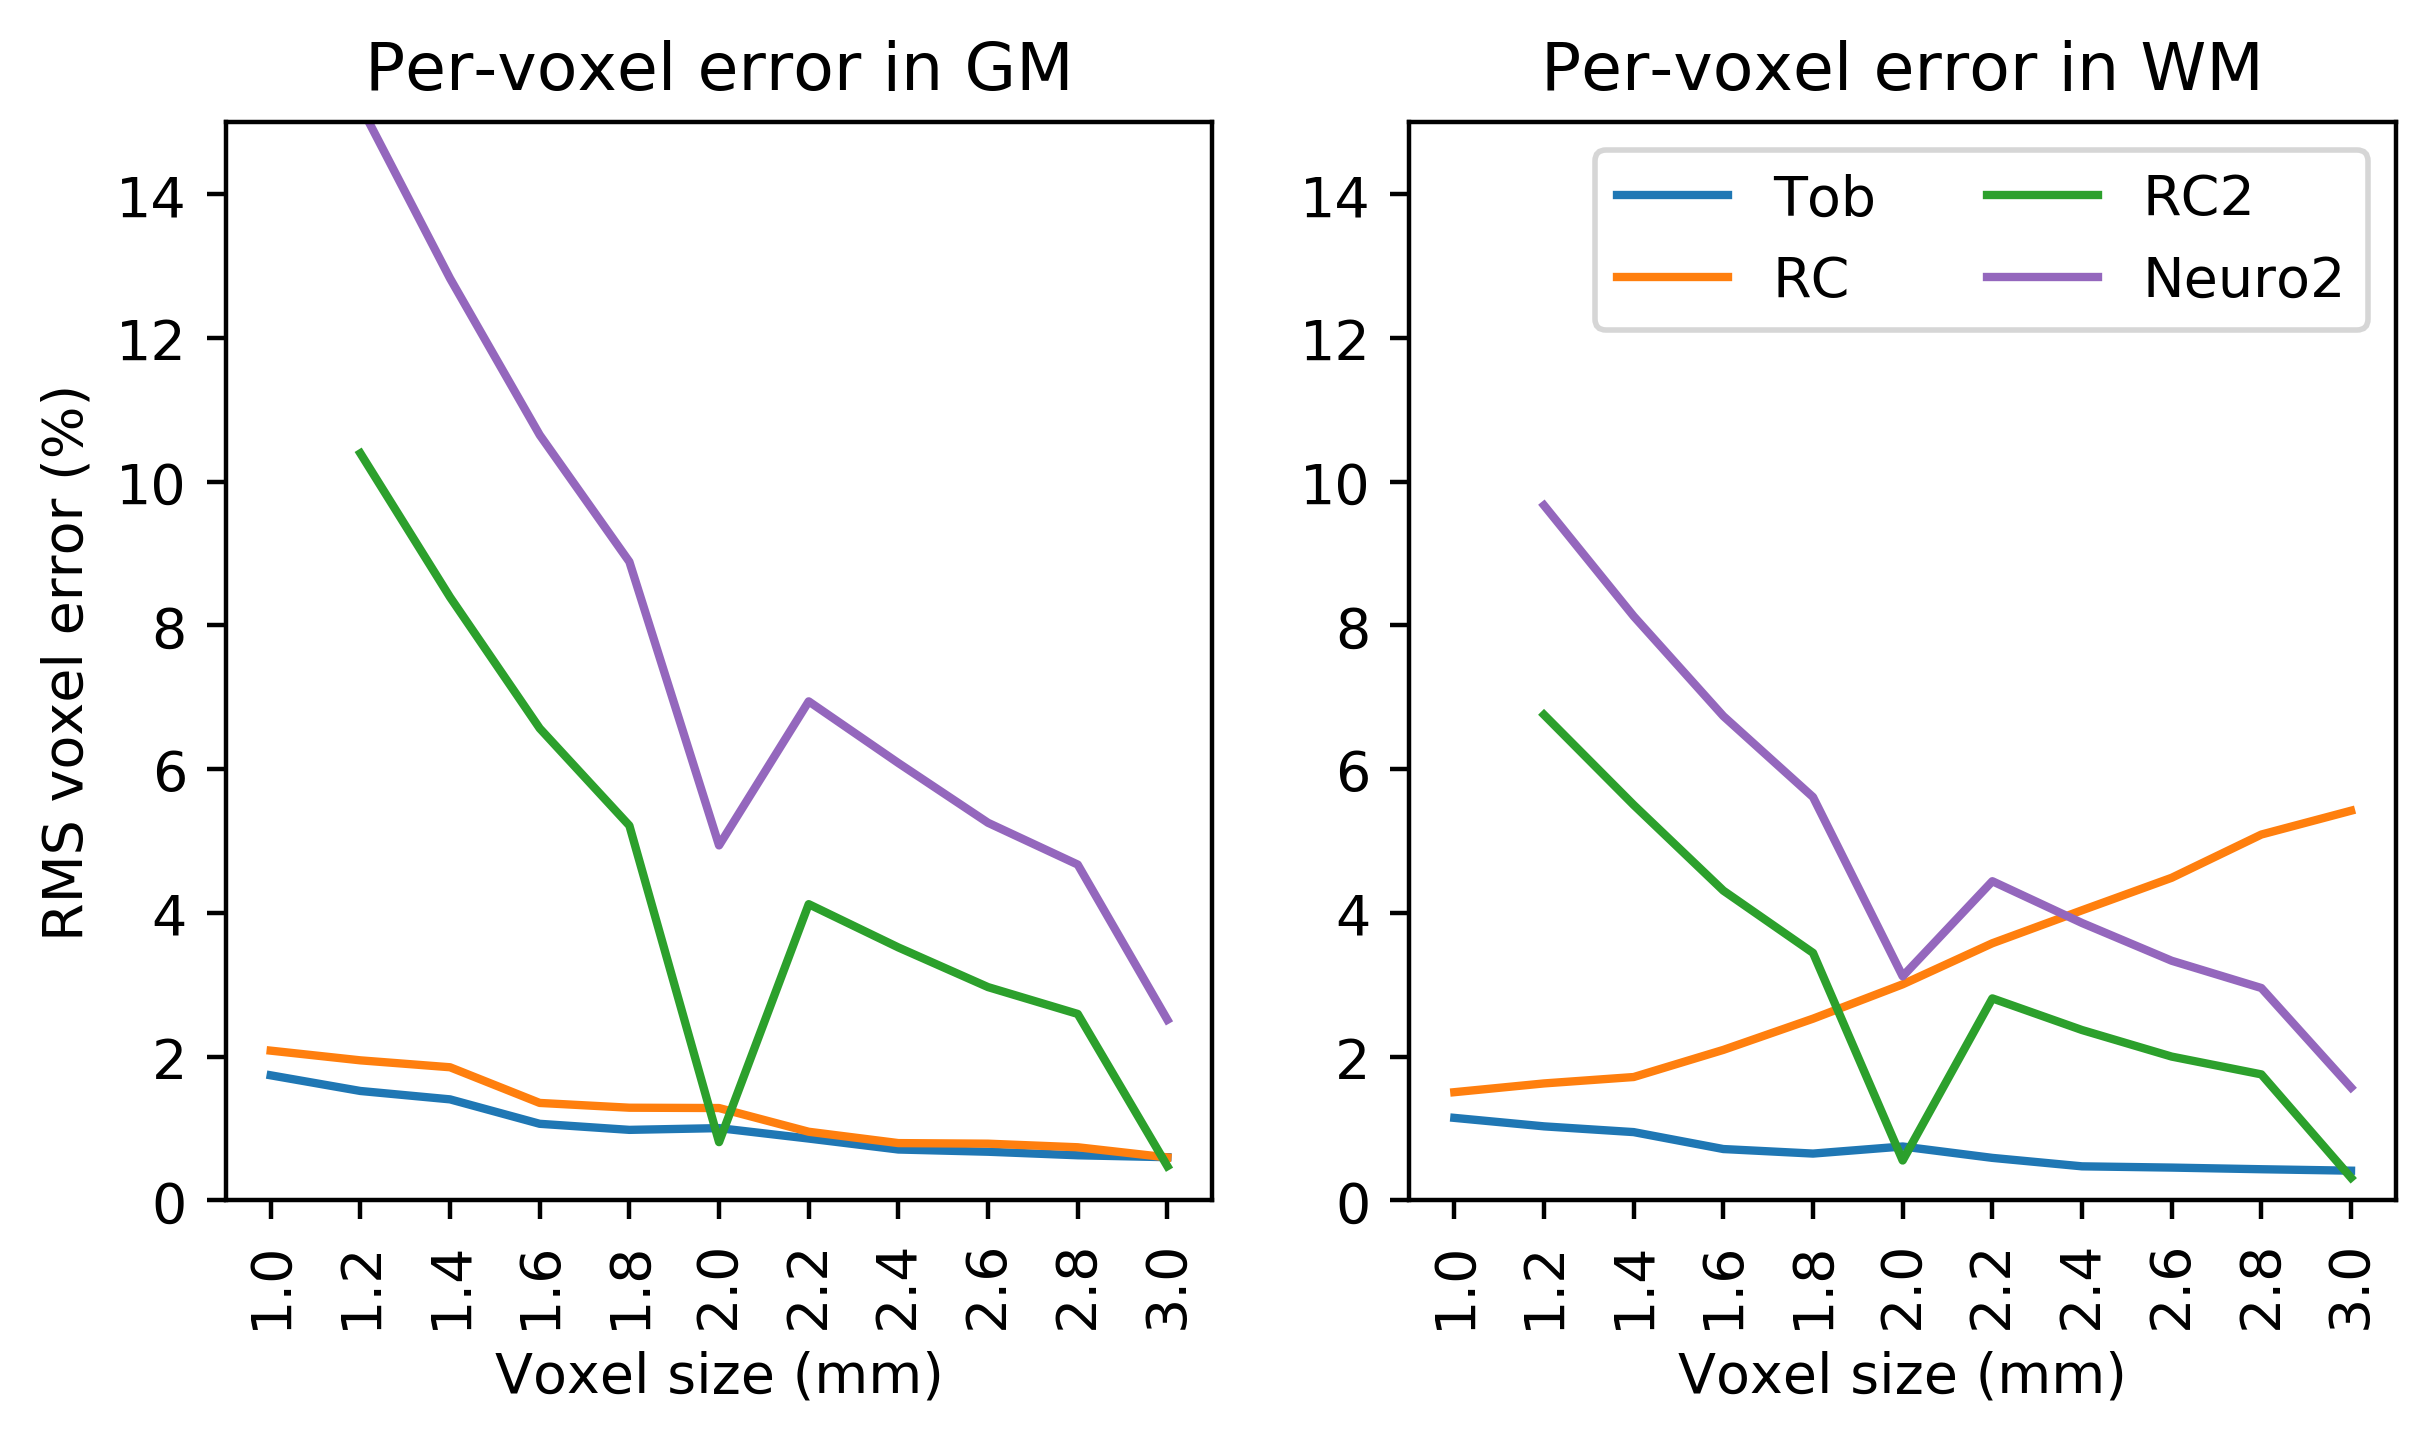
\includegraphics[width = 0.8\textwidth]{tob_sim_voxel.png}
\caption{Simulated surfaces: per-voxel error. Toblerone and RC produced the lowest errors in GM; in WM there was a clear difference to Toblerone. RC2 and Neuro2’s errors both decreased with increasing voxel size, with a characteristic notch observed at 2mm. [Full results are in the appendix, figure \ref{tob_sim_voxel_supp}]}
\label{tob_sim_voxel}
\end{figure}

Figure \ref{tob_sim_voxel} shows per-voxel error for the simulated surfaces. Results were masked to consider voxels intersecting either surface of the cortex as only these contain PVs. Toblerone and RC produced the lowest errors at all voxel sizes in GM; in WM only Toblerone retained this behaviour. Resampling-based methods (RC2, Neuro2) produced lower errors as voxel size increased, and a characteristic notch in their results was observed at 2mm. Although RC initially performed better than RC2 in WM, the inverse was true above 2mm voxel size.

\subsection{BrainWeb}

\begin{figure}[H]
\centering
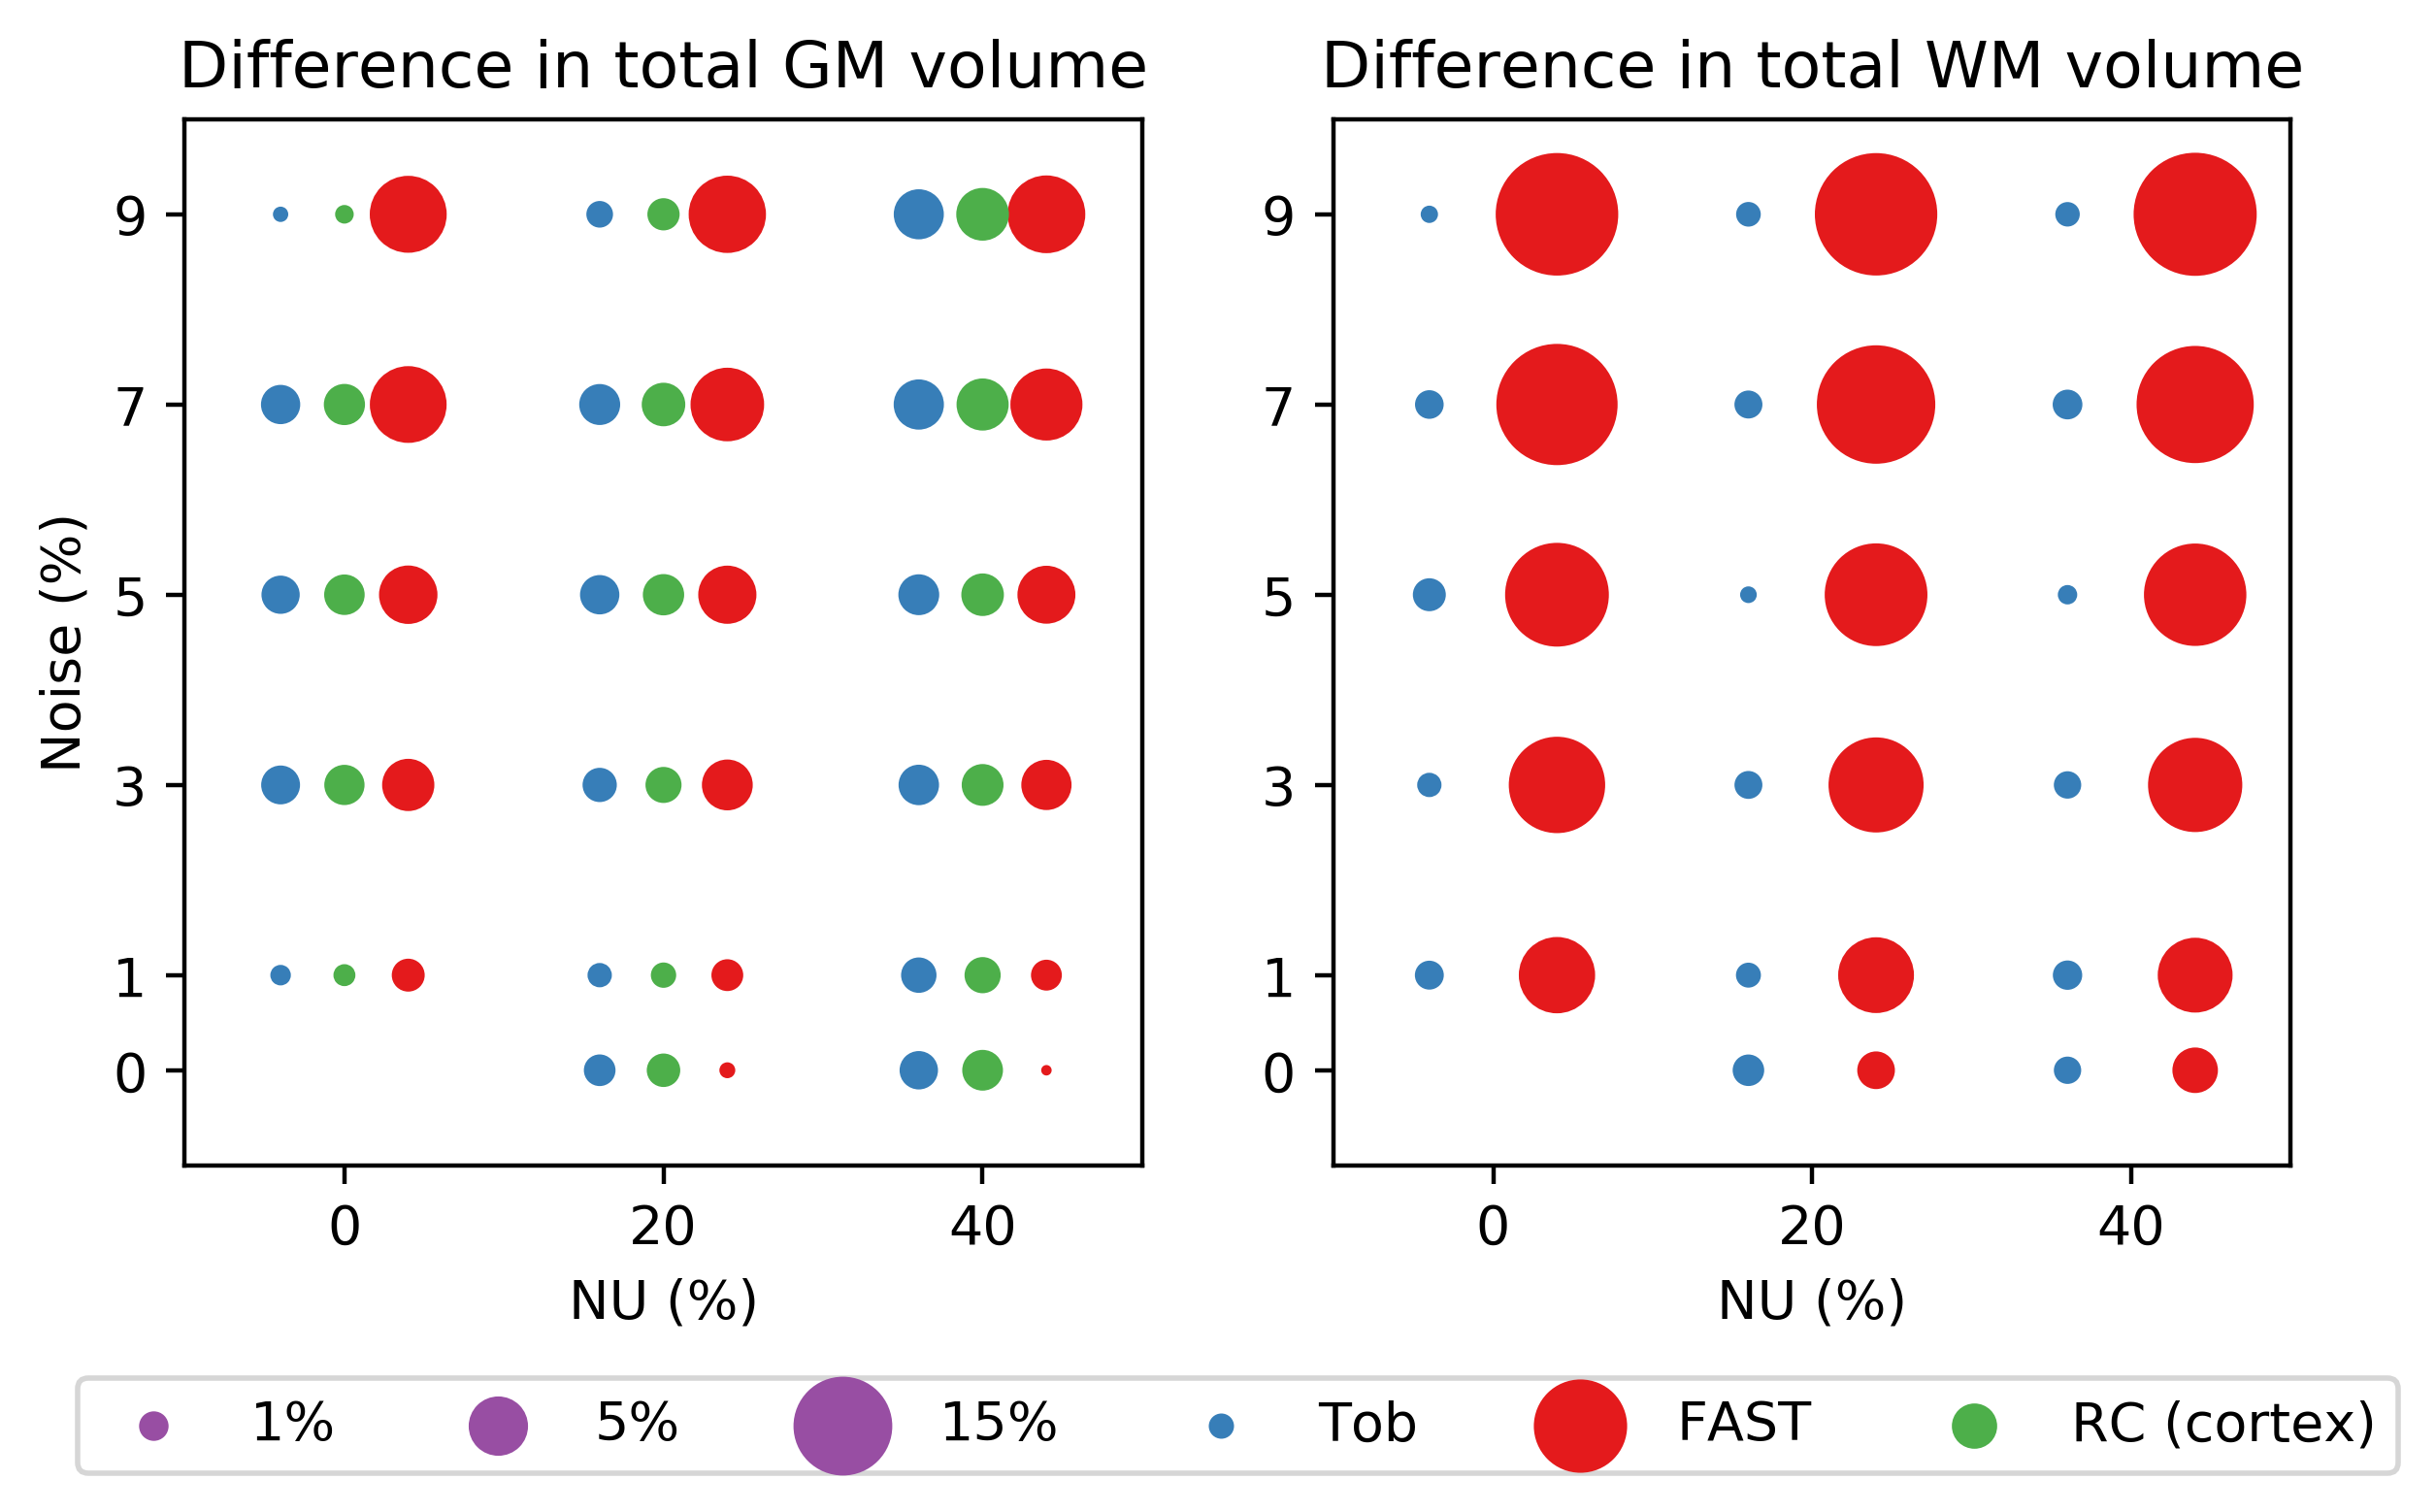
\includegraphics[width = 0.8\textwidth]{brainweb_total.png}
\caption{BrainWeb: difference in total tissue volume referenced to each method’s 0\% noise 0\% NU result. Surface-based methods were more consistent at almost all noise and NU levels; FAST was more consistent in GM than WM.}
\label{brainweb_total}
\end{figure}

Figure \ref{brainweb_total} shows the difference in total tissue volume for the BrainWeb phantom as a function of noise and NU levels, referenced to each method’s results at 0\% noise and 0\% NU. PV estimates at 1mm isotropic voxel size were used for this analysis. RC’s GM result was for the cortex only as it cannot process subcortical structures. In general, the surface-based methods showed more consistency in their estimates across all levels of noise and NU, with the notable exception of GM at 0\% noise. FAST’s consistency was notably better in GM than WM.

\begin{figure}[H]
\centering
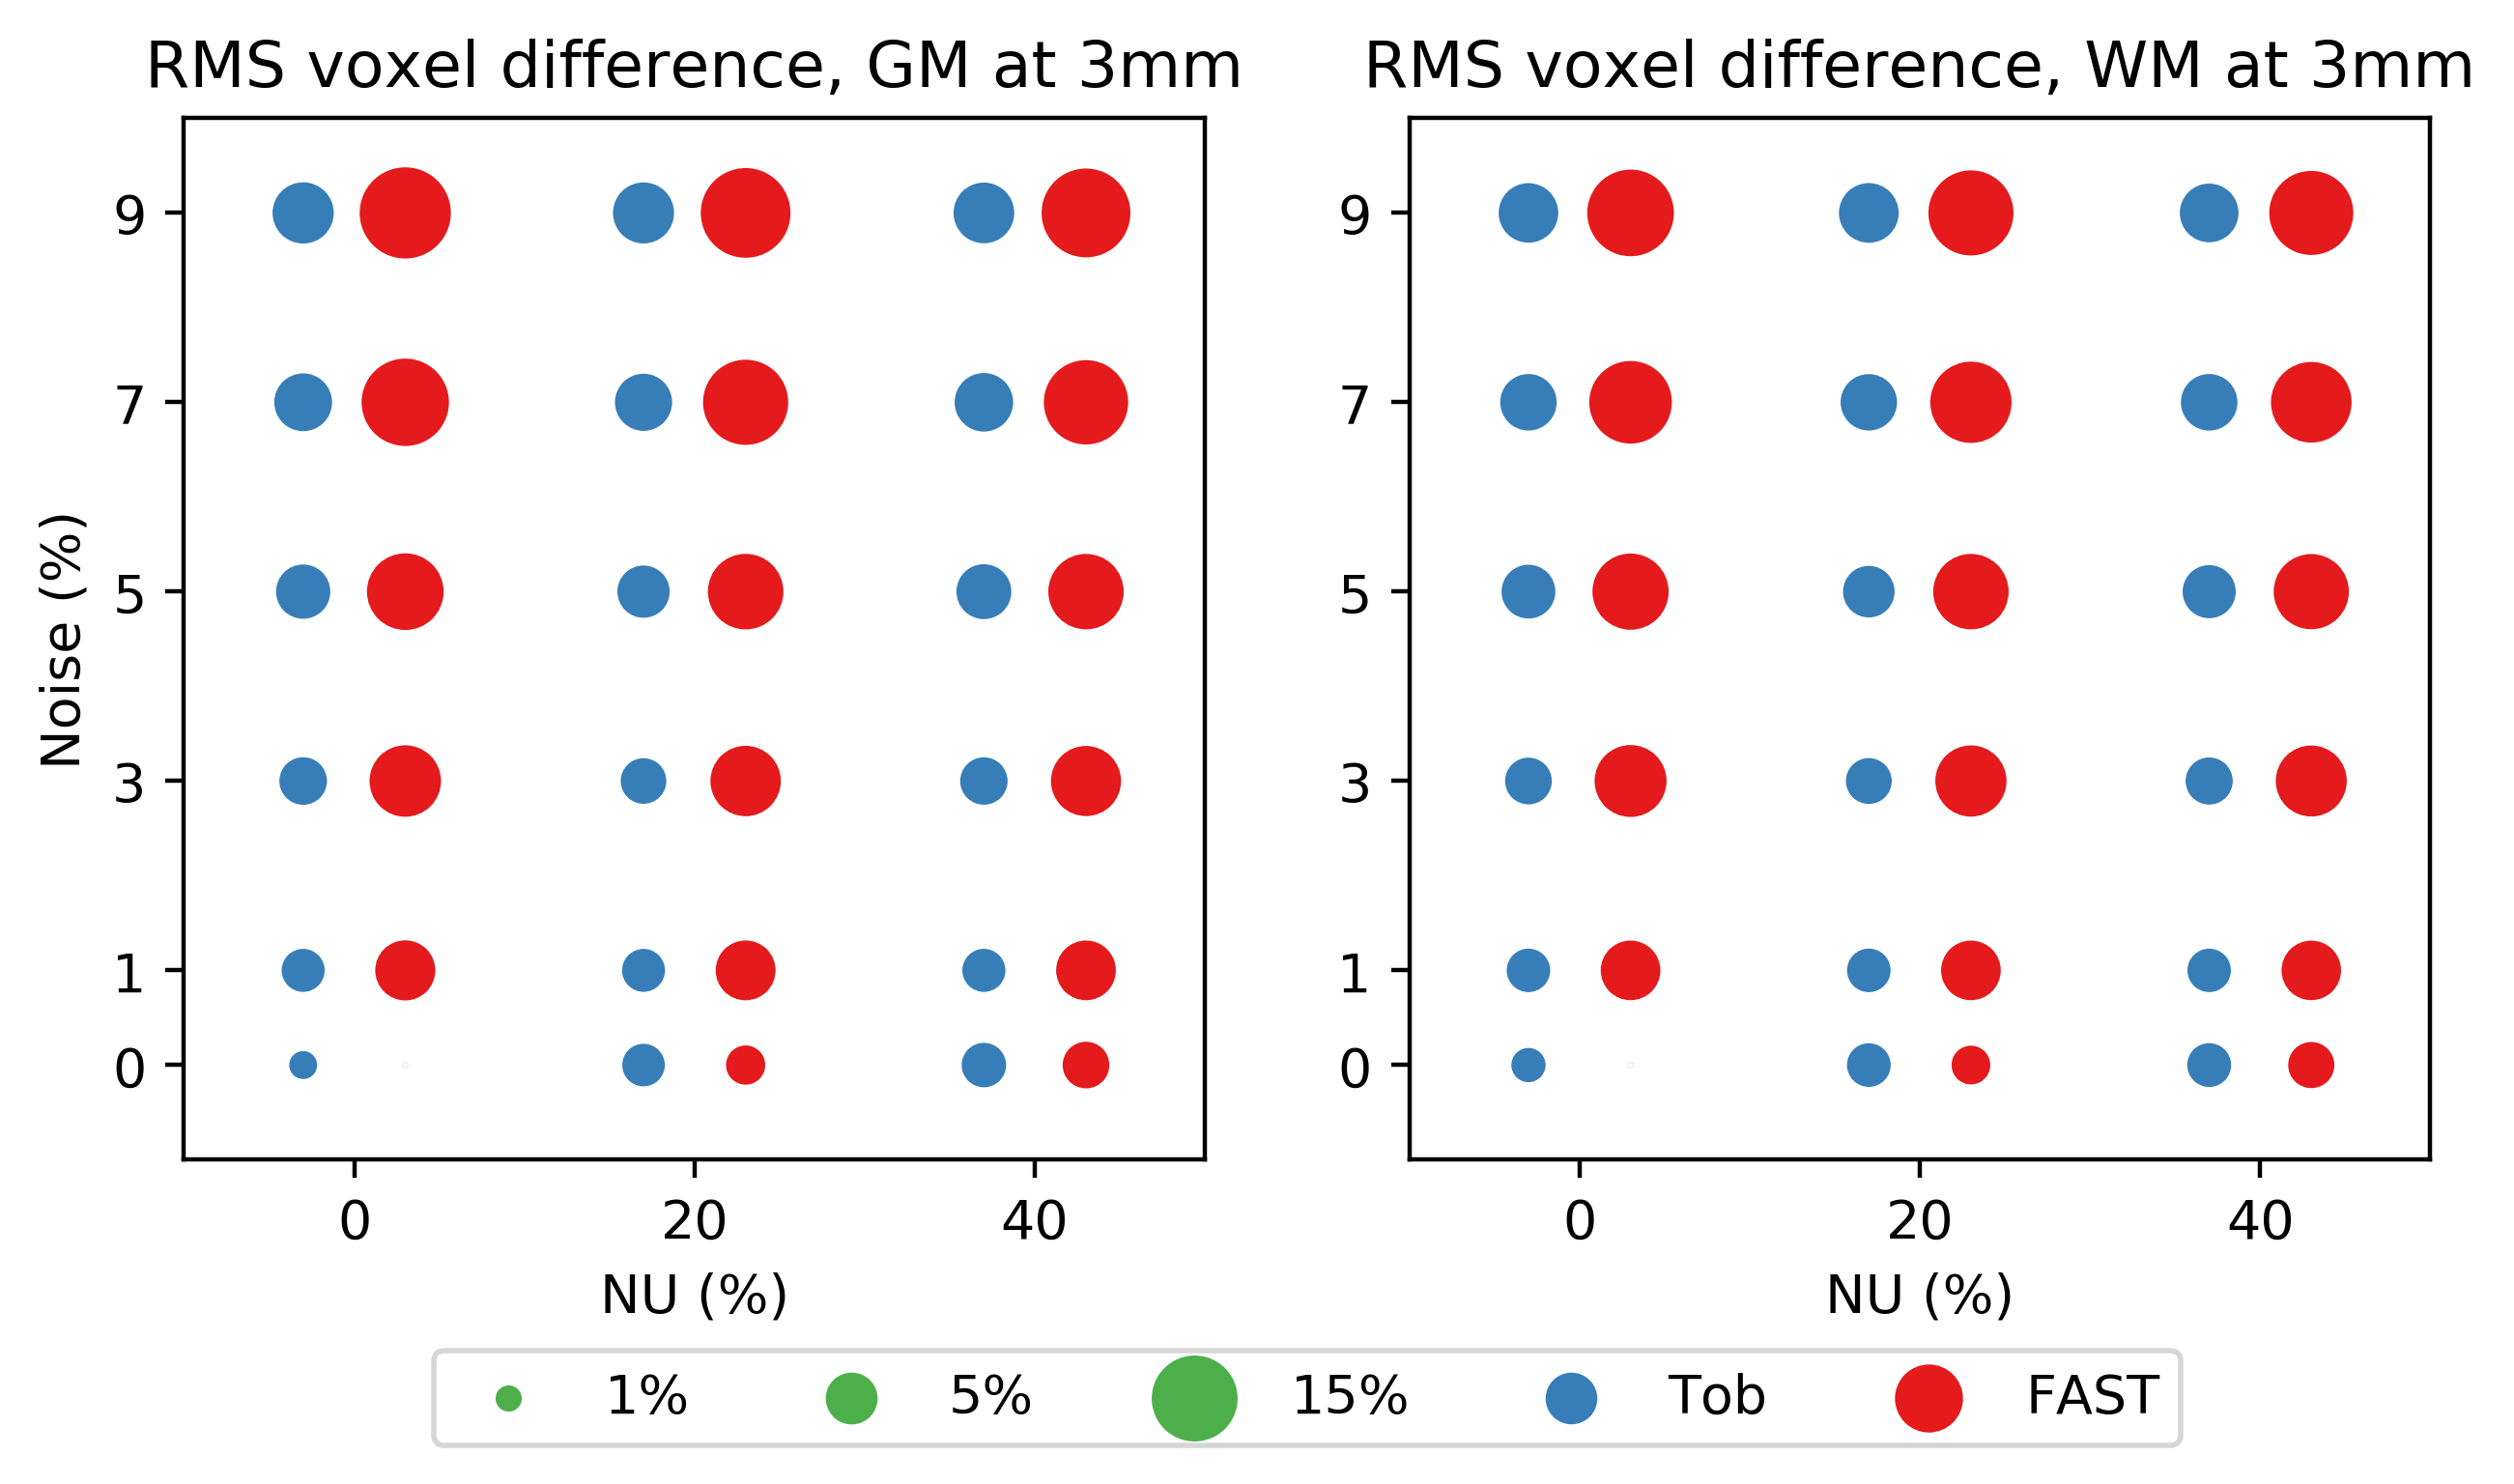
\includegraphics[width = 0.8\textwidth]{brainweb_voxel.png}
\caption{BrainWeb: RMS per-voxel differences at 3mm voxel size, referenced to each method’s 1mm 0\% noise 0\% NU results. Toblerone’s differences were smaller at almost all levels of noise and NU, as was also the case at other voxel sizes. [Results for other voxel sizes are given in the appendix, figure \ref{brainweb_voxel_supp}]}
\label{brainweb_voxel}
\end{figure}

Figure \ref{brainweb_voxel} shows the RMS per-voxel difference in PV estimates at 3mm voxel size as a function of noise and NU. Each method’s 1mm results at 0\% noise 0\% NU were used as the reference. Toblerone returned lower RMS voxel differences in both GM and WM at all levels of NU and noise except 0\% noise 0\% NU, a pattern that was repeated at other voxel sizes (given in the appendix, figure \ref{brainweb_voxel_supp}).

\subsection{HCP test-retest}

\begin{figure}[H]
\centering
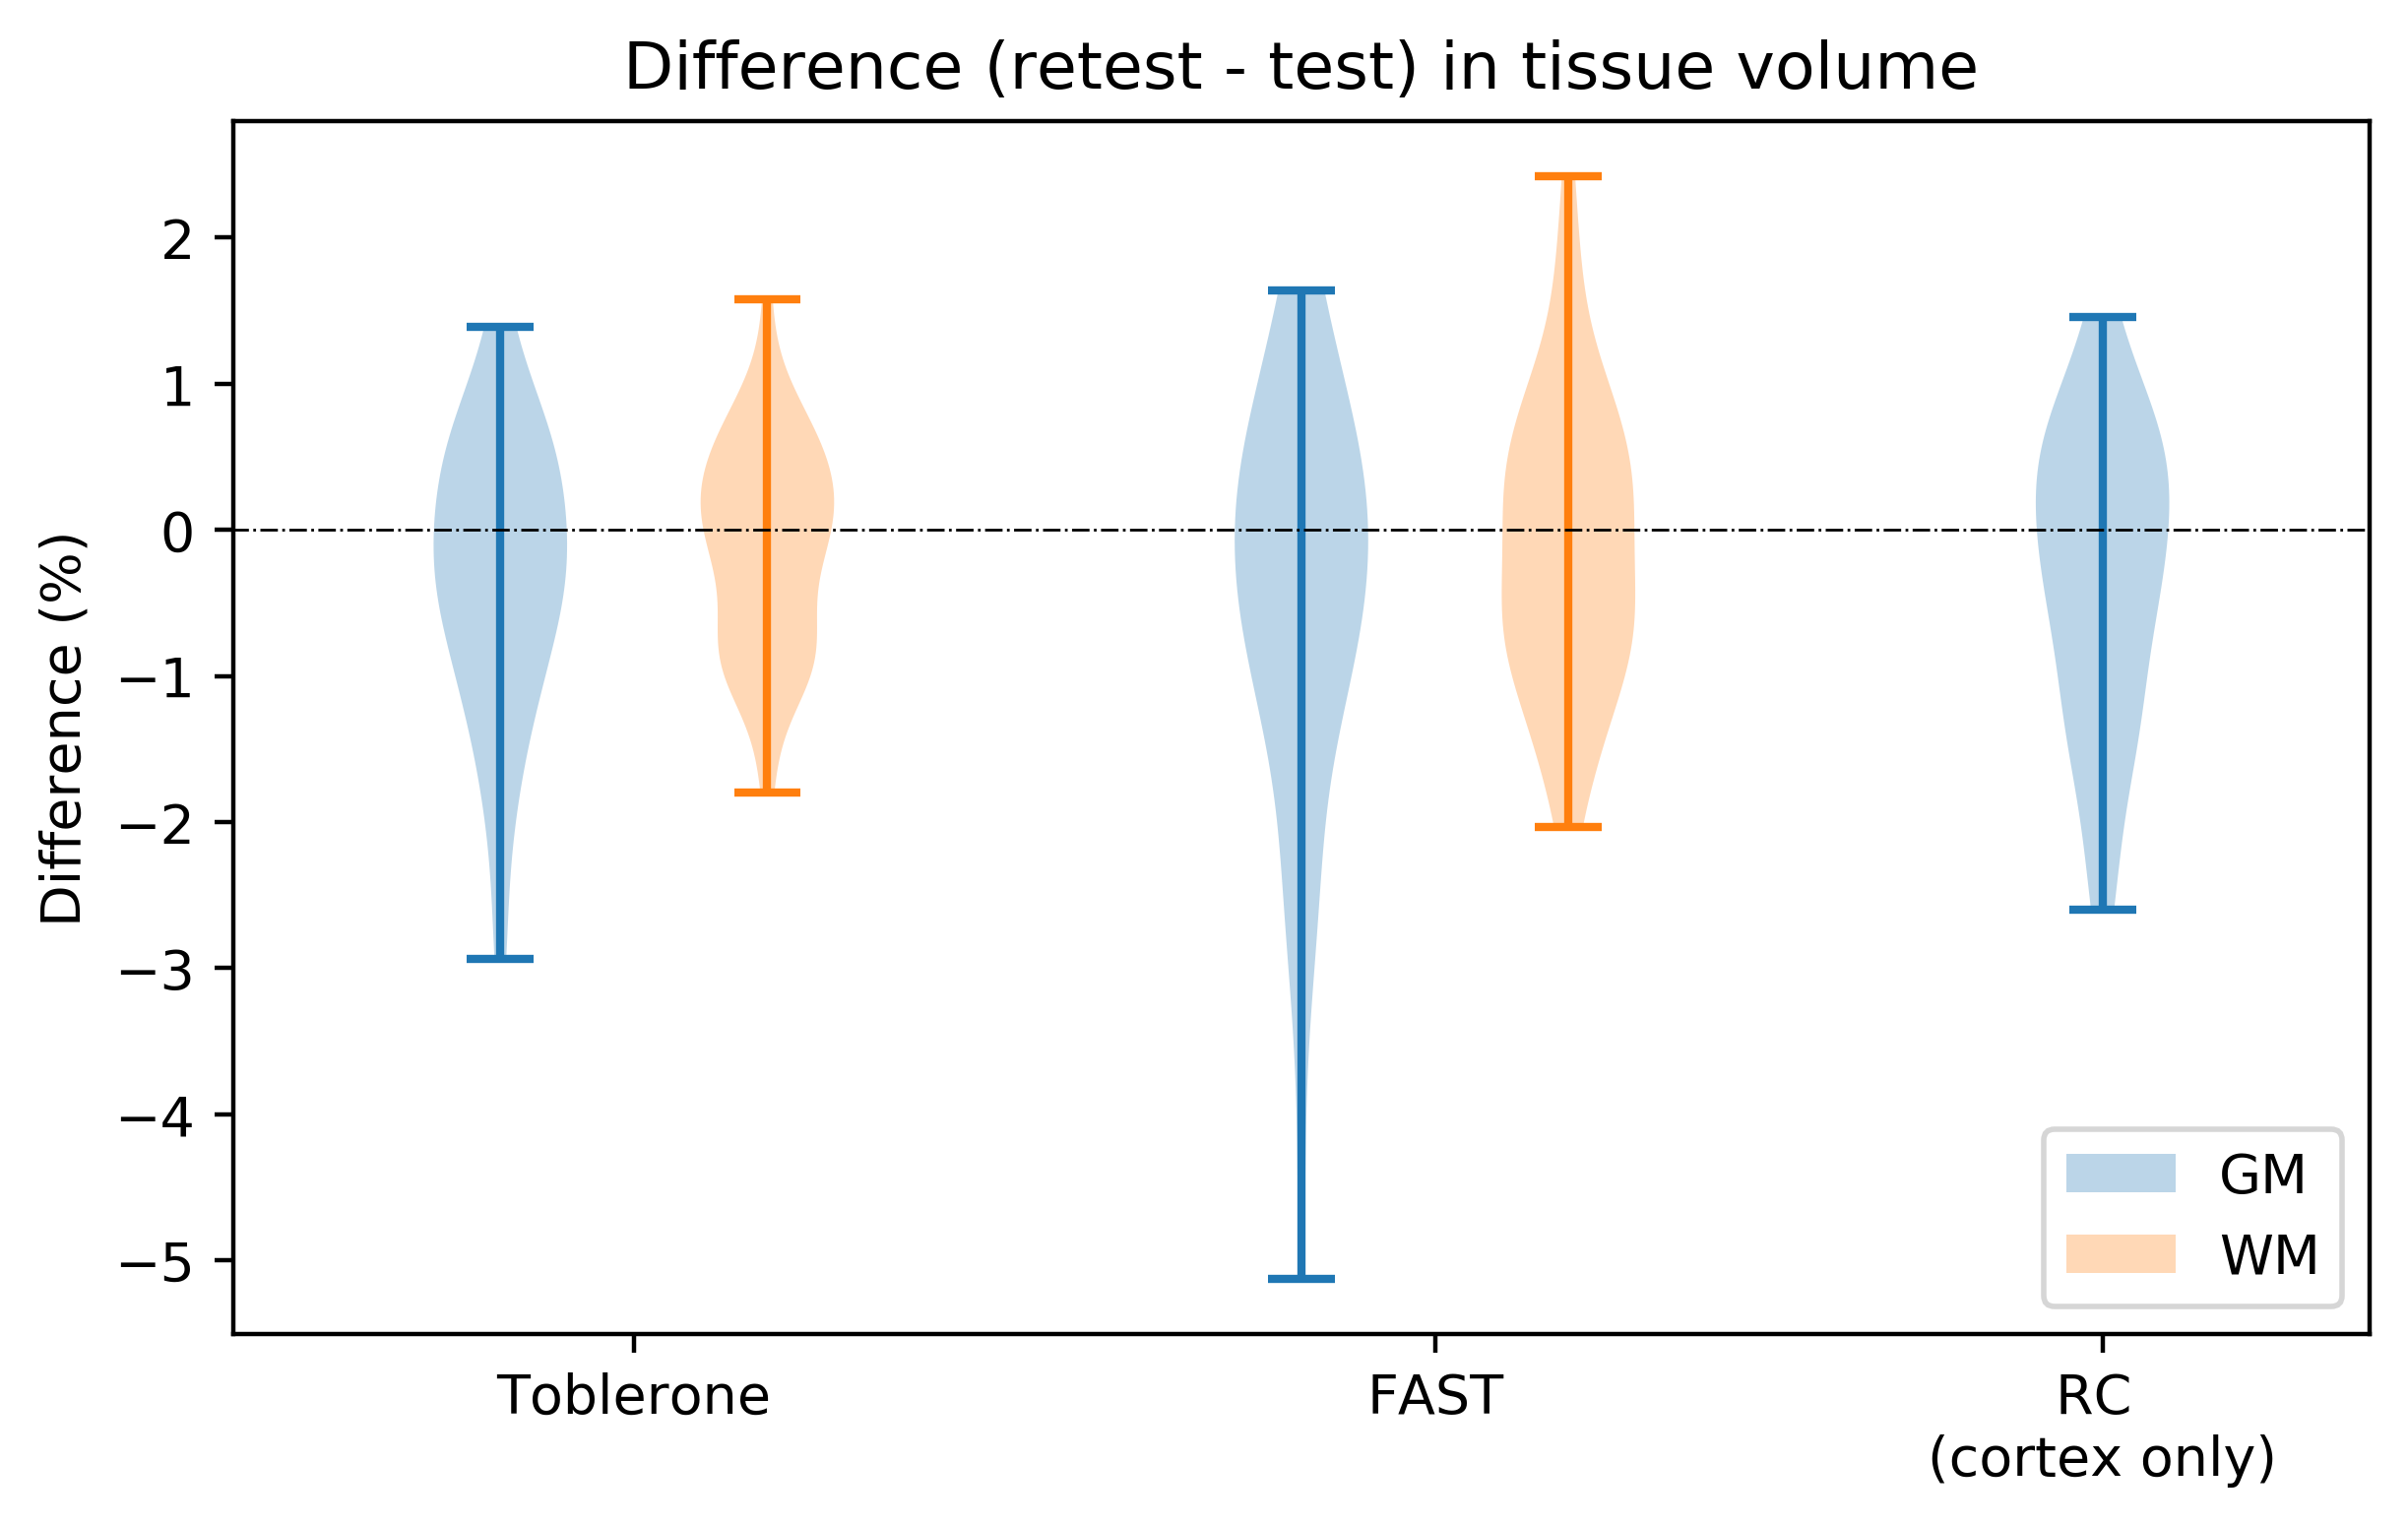
\includegraphics[width = 0.7\textwidth]{hcp_total.png}
\caption{HCP test-retest: inter-session (retest minus test) difference in total tissue volume. PVs were estimated in the native 0.7mm isotropic space of the structural images. RC’s result is for the cortex only. Both surface methods show a tighter distribution than FAST.}
\label{hcp_total}
\end{figure}

Figure \ref{hcp_total} shows violin plots of inter-session difference (retest - test) in tissue volume across the 45 subjects of the HCP dataset. PV estimates at 0.7mm isotropic voxel size were used for this analysis. RC’s GM result was for the cortex only. Both surface methods gave a tighter distribution than FAST, suggesting greater repeatability between sessions. All methods showed greater variability in GM than WM.

\begin{figure}[H]
\centering
\includegraphics[width = 0.7\textwidth]{hcp_difference.png}
\caption{HCP test-retest: mean difference between Toblerone and FAST GM PVs, sorted into 5\% width bins according to Toblerone’s GM PV. As Toblerone’s GM PV estimate in a given voxel increased, FAST was more likely to assign a smaller value, and vice-versa. The strength of this relationship decreased with increasing voxel size. An inverse, but weaker, effect was seen for WM (figure \ref{hcp_difference_wm_supp} in the appendix).}
\label{hcp_difference}
\end{figure}

Figure \ref{hcp_difference} shows the mean per-voxel difference between Toblerone and FAST’s GM PV estimates as a function of Toblerone’s GM PV estimate. Excepting the 0.7mm result, the positive slope of each line shows that in voxels with a low Toblerone GM PV estimate, FAST was more likely to assign a higher value, and vice-versa at high Toblerone GM PV estimates. The strength of this relationship decreased with increasing voxel size. It should be noted that the 0.7mm result was the only one not to make use of resampling (for all others, FAST’s 0.7mm estimates were resampled onto the target voxel grid).

\subsection{\textit{In-vivo} ASL data}

\begin{figure}[H]
\centering
\includegraphics[width = 0.8\textwidth]{tob_vs_fast_cbf_correlation.png}
\caption{\textit{In-vivo} ASL data: correlation coefficients ($R$) of uncorrected CBF vs GM PV for FAST and Toblerone. Left: correlation against both cortical and subcortical GM. Right: correlation against cortical GM only. In almost all cases, Toblerone's estimates returned higher correlation coefficients compared to FAST, with the difference in results smaller when considering the cortex only. Significance values for a paired $t$-test comparing $R$ values are shown on each plot. }
\label{tob_vs_fast_cbf_correlation}
\end{figure}

Figure \ref{tob_vs_fast_cbf_correlation} shows correlation coefficients arising from linear regressions of uncorrected CBF against GM PV for the \textit{in-vivo} ASL data. In almost all cases, Toblerone's GM PV estimates yielded a higher $R$ value than FAST, with the difference greater when considering both the subcortex and cortex together. The variation within subjects was substantially smaller than the variation between subjects. A paired $t$-test comparison was performed by averaging $R$-values within each subject to yield four samples per method; the comparison did not meet a $p <$ 5\% significance threshold (likely due to the low number of subjects considered). 

\section{Discussion}

Results from the simulated surfaces showed that Toblerone produced estimates with a comparatively low and consistent error. Although the RC method was able to perform similarly for GM, there was a clear advantage for Toblerone in WM. Results from the BrainWeb dataset suggested that a surface-based approach (the combination of FreeSurfer/FIRST and Toblerone) was more robust to random noise and field non-uniformity than FAST’s volumetric approach. In particular, the BrainWeb results showed that the consistency of FAST’s WM estimates suffered in the presence of these real-world imperfections. Results from the HCP test-retest dataset showed that the surface-based approach provided better inter-session repeatability in estimates of total tissue volume. Finally, results from the \textit{in-vivo} ASL data demonstrated a positive trend (albeit below statistical significance) that Toblerone's PV estimates correlated better than FAST's with PVE-corrupted CBF. The difference in performance was greater when considering both the subcortex and cortex together versus the cortex only; it is known that FIRST and FAST take different views regarding the tissue composition of subcortical structures. Whilst this result does not imply that Toblerone's estimates are more `correct' than FAST's, it does suggest that a surface-based approach is better able to explain PVE-induced variation within physiological imaging data, which in turn could enable improved PVEc. 

In its native form, the RC method is unable to correctly handle voxels in which all three tissue types are present (due to the fact that it estimates only GM and then leaves the user to assign the remainder as WM or CSF based on some heuristic). The impact of this was seen in the positive relationship between per-voxel error in WM and voxel size in figure \ref{tob_sim_voxel}. Resampling can help to minimise this error: at small voxel sizes, the probability of voxels containing three tissue types is smaller and so the error is minimised, but this does not hold true at larger voxel sizes. Accordingly, as output voxel size increases, it is increasingly beneficial to obtain PV estimates by resampling those from a smaller voxel size. Set against this, however, are the aforementioned problems introduced by resampling: when the ratio of output to input voxel size is small, subvoxel effects are significant and high per-voxel errors result (as seen in figure \ref{tob_sim_voxel}). A threshold voxel value above which resampling is beneficial therefore results (at around 2mm in the figure). The exact value of this threshold would be difficult to predict in the general case (in particular, the use of aligned voxel grids in this work is both highly significant and extremely unrealistic). By contrast, Toblerone is able to produce consistent estimates in all tissue classes at arbitrary voxel sizes without the use of resampling. 

\DIFaddbegin \DIFadd{Figure \ref{hcp_difference} suggested that FAST's PV estimates were biased towards the centre of the unit interval (at least, when compared Toblerone's). For example, in a voxel that Toblerone estimated to have a low GM PV, FAST estimated a higher value, and vice-versa: in both cases, FAST's estimate was closer to the mid-point of 50\% than Toblerone's. This is possibly explained by the fact FAST uses a probability-based approach, and values in the mid-point of the interval are more likely than those at the extremes. By contrast, Toblerone's approach is purely geometric and has no knowledge of which values are more probable than others. 
}

\DIFaddend It was not possible to further analyse the HCP test-retest dataset in order to establish where in the brain the differences between Toblerone’s and FAST’s estimates arise. To do so would require extensive use of non-linear registrations and resampling to transform all subjects onto a common template, and it is likely that the artefacts imposed by this process would obscure the true methodological differences of interest. Furthermore, an analysis on the BrainWeb database would be of limited use as it only represents the cortical anatomy of a single subject and would therefore ignore population variability.

\section{Conclusion}

A new method (Toblerone) has been presented for estimating PVs using surface segmentations. Unlike existing surface-based tools, it is not closely tied to any specific modality or structure and can therefore be adapted to multiple use cases (notably, providing PV estimates for the whole brain). It is able to operate at arbitrary resolutions without recourse to resampling, thereby avoiding the highly localised degradation of image quality that this process entails. Four datasets have been used for evaluation of the method. Results from simulated surfaces show consistently low errors at both the voxel and aggregate level, either matching or surpassing other surface-based methods. Results from simulated T1 images from the BrainWeb database show that a FreeSurfer/FIRST/Toblerone surface-based pipeline used as an alternative to FAST is more robust in the presence of random noise and field non-uniformity. Results from the HCP test-retest dataset of 45 subjects show that the surface-based pipeline produces a tighter distribution of inter-session tissue volumes than FAST, suggesting the surface approach has greater repeatability. Finally, a preliminary investigation using \textit{in-vivo} ASL data offers a promising hint that surface-derived estimates are better able to explain PVE-induced variation within physiological imaging data. Further analysis with a larger dataset will be required to confirm the latter result. 
 \newpage 
 \newpage % Activate the following line by filling in the right side. If for example the name of the root file is Main.tex, write
% "...root = Main.tex" if the chapter file is in the same directory, and "...root = ../Main.tex" if the chapter is in a subdirectory.

% !TEX root = ../thesis.tex 

\chapter{Cortical surface projection of volumetric data}
\label{projection_chapter}

\section{Introduction}

Surface-based methods can offer advantages for the analysis of physiological imaging data from particular anatomical structures. As applied to the cortex, previous work has shown that they can facilitate improved localisation of functional areas within subjects and better registration between subjects compared to conventional volumetric methods \cite{Glasser2016, Coalson2017}. Whilst some modalities lend themselves naturally to surface-based analysis (notably EEG), those that acquire volumetric data require an extra processing step to transform the data into the surface space. This is true of all MRI based methods, including BOLD fMRI (for which a number of projection methods exist), and ASL (for which little prior work exists that is specific to the modality). 

The projection framework that is developed in this chapter (incorporated into the Toblerone package and hereafter referred to by that name) is intimately tied to the combined surface and volumetric inference framework that will be introduced in chapter \ref{svb_chapter}. Whilst it can be used as a standalone tool in a manner comparable to existing methods, the principles on which it is built (in particular, hybrid space) are best understood in the context of the analysis framework that will follow. 


\subsection{Objectives}

Three existing projection methods for BOLD fMRI were introduced in section \ref{lit_projection_methods}. Whilst any of these could in principle be made to operate with other modalities, such as ASL, they all share the common property of encoding assumptions about the BOLD signal within their formulations. This is of vital importance as the assumptions cannot necessarily be carried across to other modalities. Considering ASL, for example, the point of divergence is signal from WM. In BOLD, it is assumed that little signal originates in WM, and that which does is often treated as noise. For a modality such as ASL, WM does generate a signal of interest (albeit weaker and therefore more difficult to analyse than GM), and it should therefore not be neglected or discarded. Furthermore, the space in which analysis is performed is of vital importance: though it  makes sense to analyse cortical signal in a surface-based manner, this is not true of WM signal, and so what is ultimately required is projection framework that both acknowledges the existence of signals arising from multiple tissues, \textit{and} allows for the analysis of these signals in the space that is best suited for them (cortical on the surface, subcortical in the volume).  

Whilst the core of this framework shares many features in common with the HCP's ribbon-constrained (RC) method, a number of important changes have been made. The end result can be used in two different ways. Firstly, it can be used in a narrow sense to perform volume-surface projection in a manner comparable to RC (and offering small improvements in performance). Secondly, it can be used in its novel form to project data to and from a hybrid space as part of a process of parameter estimation. Used in this manner, significant improvements in performance compared to the RC method are observed, though it is acknowledged that the comparison is imperfect as the RC method is not designed for this purpose. \DIFaddbegin \DIFadd{The respect in which this framework differs most from existing projection methods is in its application to parameter estimation. Conventional methods emphasise the projection of volumetric timeseries data onto the surface, after which some modality-specific analysis is performed (independently of the projection). By contrast, this framework emphasises the }\textit{\DIFadd{reverse}} \DIFadd{projection, from surface back to volume, which is incorporated into a modality-specific parameter estimation framework (in fact, the estimation }\textit{\DIFadd{requires}} \DIFadd{the reverse projection to function). This will be expanded upon in the following chapter. 
}\DIFaddend 

\subsection{Hybrid space}

The terms \textit{volume}, \textit{surface} and \textit{hybrid} space will be used throughout this chapter. These are used to refer to the space of representation of data. For example, voxel-wise data is in volume space; vertex-wise data on the cortical surface is in surface space; and data that has both a voxel- and vertex-wise representation is in hybrid space. 

The concept of hybrid space is of fundamental importance to this projection framework. It follows directly from the aforementioned use case for this method, which is to perform physiological parameter estimation for both the cortex and subcortex simultaneously, hereafter referred to as \textit{hybrid inference}. The spatial locations within the brain at which estimation is to be performed are termed \textit{nodes}, hence, within hybrid space the set of all nodes is defined as all surface vertices ($\vec{p}_L$ and $\vec{p}_R$ for the left/right hemispheres of the cortex) and all voxels ($\vec{v}$) of interest. 

\begin{equation}
\vec{n} = [\ \vec{p}_L \ | \ \vec{p}_R \ | \ \vec{v} \ ] 
\end{equation} 

Hybrid space permits parameter estimation in the space most suited to the structure in question: cortical parameters are estimated on the surface and subcortical parameters are estimated within voxel space. As far as is permitted by the available anatomical information (surface segmentations and volumetric masks), the defining principle of hybrid space is that each node should only correspond to one tissue. Voxels that contain both cortical and subcortical partial volumes will therefore contain \textit{multiple} nodes: one for each surface vertex and one for the voxel centre itself. This is an embodiment of the partial volume effect (the presence of multiple sources in a single voxel) and is illustrated in figure \ref{voxel_node}. The CIFTI file format \cite{cifti} embodies a similar principle to this definition of hybrid space, whereby cortical data is stored in a vertex-wise manner on the surface and subcortical data is stored in a voxel-wise manner, all within the same structure.

\begin{figure}
\centering
\includegraphics[width=0.5\textwidth]{voxel_node.png}
\caption{Schematic representation of voxels and nodes. The primitives comprising the cortical ribbon are denoted with brown boundaries. Voxel boundaries and centres are in black, labelled $v_1$ to $v_4$. Nodes are in red; $n_1$ to $n_6$ are cortical (corresponding to surface vertices), $n_7$ to $n_{10}$ are subcortical (corresponding to voxels). Individual voxels may contain multiple nodes, which is an explicit representation of PVE.}
\label{voxel_node} 
\end{figure}

As nodes in hybrid space correspond to only one tissue, the signals associated with them must also respect this distinction. Signal on cortical nodes is considered as being purely cortical (i.e., GM) in origin, and signal on subcortical nodes is considered as purely subcortical in origin (i.e., WM or a subcortical GM structure). \textit{How} these separate signals are derived from data that contains PVE is beyond the scope of this chapter (and is in fact the objective of PVEc)\footnote{Though many projection methods acknowledge the existence of PVE within data, there is little that can be done to rectify this during the narrow operation of projection. To do so would require a basis on which to separate cortical and subcortical contributions, which is the purpose of PVEc itself and therefore a non-trivial operation.}. For the purposes of this work, it is only necessary to posit that the separate signals exist and that their representation respects their separation. When projecting from hybrid to volume space, the process of PVE must therefore be recreated to mix the separate signals within each voxel. It is this specific projection, incorporating PVE, which facilitates the performance of surface-aware parameter estimation as it allows for the reconstruction of volumetric data from a set of cortical and subcortical parameter estimates. This will be addressed in chapter \ref{svb_chapter}. 

Whilst projection to and from hybrid space, for the purpose of performing hybrid inference, is the intended use case of the work presented in this chapter, Toblerone's projection can be made to operate in a conventional surface-volume sense. In this form, a projection that is directly comparable to existing surface-volume methods is recovered. 

\section{Construction of the projection}

The projections described herein can be performed with either one or both cortical hemispheres at a time. The forward and reverse projections are constructed from the same two matrices. Conceptually, these perform a transformation between voxels and surface triangles, and then between surface triangles and surface vertices. The cortical midsurface (exactly halfway in between the white and pial surfaces) is used by default, though this could be modified for other use cases (such as laminar fMRI). A set of PV estimates for the cortex is also used; these are produced using Toblerone's PV estimation function operating on the cortical surfaces, as detailed in chapter \ref{tob_pv_chapter}.

\subsection{Voxel-triangle matrix}
The voxel-triangle matrix records the intersection between individual voxels and the volume primitives that comprise the cortex. The problem is approached in a triangle-wise manner, as opposed to vertex-wise, as this allows for the construction of extremely simple primitives. Triangle correspondence between the inner (white) and outer (pial) surfaces of the cortex is assumed. For each pair of triangles, their corresponding vertices are connected to form a triangular prism\footnote{Or, even better, a Toblerone bar, hence the name.} which is then subdivided into three non-overlapping tetrahedra \cite{Dompierre1999}. For example, for triangles with vertices $\triangle ABC$ and $\triangle abc$ on the pial and white surfaces respectively, the prism may be split as $ABCa$, $Cabc$ and $BCab$. As a consequence of this subdivision, each rectangular face of the prism will be split along the diagonal into two triangles. It is important to ensure that the orientation of this face diagonal is consistent between neighbouring prisms so as to avoid producing overlapping tetrahedra. This is achieved by fixing the direction of subdivision according to the ordering of vertex numbers: `positive' if $A < B$, $B < C$ or $C < A$, and `negative' otherwise. 

Subsequently, for each voxel in the neighbourhood of the prism, an isotropic grid of sample points is initialised. Figure \ref{prism} shows one such prism and the sample points from one neighbourhood voxel. These points are tested to determine if they lie within each tetrahedra (via the Delaunay triangulation \cite{Barber:1996:QAC:235815.235821}) and the fraction that do are recorded in $\mat{VT}$, a matrix sized (voxels x triangles). 

\begin{equation}
\mat{VT} = 
\begin{bmatrix}
vt_{11} & \ldots & vt_{1t} \\
\vdots & \ddots & \vdots \\
vt_{v1} & \ldots & vt_{vt}
\end{bmatrix}
\end{equation}

The elements $vt_{vt}$ are continuous values in the range [0,1] recording the fraction of sample points from voxel $v$ that lie inside triangular prism $t$. This matrix is highly sparse: for a voxel size of 2.2mm isotropic and a surface resolution of 32k vertices, each triangular prism intersects around 10 voxels on average.

\begin{figure}[H]
\centering
\subcaptionbox{\label{prism1}}[0.45\textwidth]
{\includegraphics[width=0.45\textwidth]{prism4}}
\subcaptionbox{\label{prism2}}[0.45\textwidth]
{\includegraphics[width=0.45\textwidth]{prism1}}
\caption{Two alternative views of the triangular prism (purple) formed by connecting one pair of corresponding triangles on the inner and outer surfaces (grey) of the cortex. The subdivision into three tetrahedra is not shown. A $5^3$ grid of sample points are tested to determine the volume of intersection between the voxel and prism, which is recorded in the voxel-triangle matrix.} 
\label{prism}
\end{figure}

This approach is very similar to that of Toblerone's PV estimation algorithm from chapter \ref{tob_pv_chapter}, which uses convex hulls to determine the volume of intersection between a patch of surface and a voxel. There is however a subtle but important distinction. Toblerone's PV estimation estimates the total amount of cortical tissue per \textit{voxel}. This is a reduction operation that sums together all of the contributions of the surface primitives within a given voxel. By contrast, this process estimates the contributions of neighbourhood voxels per \textit{surface primitive}, which is the other way around and does not involve a reduction operation. 

\subsection{Points-triangle matrix}
The points triangle matrix records the area of each triangle on the cortical midsurface that `belongs' to its individual vertices (though vertices are now referred to as points to avoid re-using the letter $v$). These values are calculated using the Voronoi region approach, extended to arbitrary meshes by Meyer \textit{et al.} \cite{Meyer2003}, and are recorded in the matrix denoted $\mat{PT}$, sized (points x triangles). 

\begin{equation}
\mat{PT} = 
\begin{bmatrix}
pt_{11} & \ldots & pt_{1t} \\
\vdots & \ddots & \vdots \\
pt_{p1} & \ldots & pt_{pt}
\end{bmatrix}
\end{equation}

The element $pt_{pt}$ denotes the area of triangle $t$ that belongs to point $p$. Once again, this matrix is highly sparse as each point is associated to only a few triangles. 

\subsection{Forward projection}

\subsubsection{Volume to surface}
To form the volume to surface projection, the voxel-triangle matrix and point-triangle matrices are first normalised in a row or column-wise sense. This operation is denoted with the $\left\Vert \cdot \right\Vert_{row}$ operator defined below and rescales all rows or columns with non-zero sum such that they sum to unity. 

\begin{eqnarray}
\left\Vert \cdot \right\Vert_{row} &:& \mathrm{A}^{n \times m} \rightarrow \mathrm{A}^{n \times m} \nonumber \\
(\left\Vert \mathrm{A}^{n \times m} \right\Vert_{row})_{ij} &=&
\begin{cases}
a_{ij} / \sum^m_{k=0} a_{ik} & \text{if } \sum^m_{k=0} a_{ik} > 0 \\ 
0 & \text{if } \sum^m_{k=0} a_{ik} = 0 
\end{cases}
\end{eqnarray}

For the $\mat{VT}$ matrix, this is equivalent to ensuring that the sum of voxel weights for each triangle is unity, and for the $\mat{PT}$ matrix, that the sum of triangle areas for each point is unity. The effect of this is to turn these individual projections into weighted-averaging operations that preserve signal intensity. The overall projection is then defined by the multiplication

\begin{equation}
\mathrm{VS} = \left\Vert\mathrm{PT}\right\Vert_{row} \left\Vert \mathrm{VT} \right\Vert_{col}^T
\end{equation}

\subsubsection{Volume to hybrid}

In order to extend the forward projection into hybrid space, it is necessary to include the mapping between voxels and subcortical nodes (the $\mat{VS}$ matrix accounts only for cortical nodes). This is achieved by concatenating the $\mat{VS}$ matrix with the identity $\mat{I}_v$ matrix of size (number of voxels) to yield $\mat{VH}$, as illustrated in figure \ref{v2n_mat}. This implies a one-to-one mapping for all voxels to their hybrid space counterpart. 

\begin{equation}
\mathrm{VH} =  \begin{bmatrix}
    \begin{array}{c}
  \mathrm{VS}  \\
  \hline
  \mathrm{I}_v \\
    \end{array}
  \end{bmatrix}
\end{equation}

\subsubsection{Edge up-scaling}

Depending on the nature of the data that is to be projected, edge up-scaling is an optional extra step that can be incorporated into the forward projection. For signals that scale directly with the amount of tissue in a voxel, signal magnitude will be artificially low in any edge voxels that are less than 100\% brain (for example, those that contain some CSF which does not contribute any signal). In this case, it may be advantageous to up-scale the signal to account for the `lost' intensity. This is performed by calculating the voxel-wise brain PV (the sum of GM and WM PVs), taking the inverse of this quantity, and finally taking the outer product with the volume to surface projection matrix. The $\otimes$ operator denotes the outer product of a matrix and vector, in this case multiplying the \textit{j}th column of a matrix by the \textit{j}th value in a vector (referred to as `broadcasting' in NumPy or MATLAB). 

\begin{equation}
u_{i} = 
\begin{cases}
(\vec{pv}_{gm,i} + \vec{pv}_{wm,i})^{-1} & \text{if } \vec{pv}_{gm,i} + \vec{pv}_{wm,i} > 0 \\ 
0 & \text{if } \vec{pv}_{gm,i} + \vec{pv}_{wm,i} = 0 
\end{cases}
\end{equation}

\begin{equation}
\begin{aligned}
\otimes : \vec{b}^m, \mathrm{A}^{n \times m} \rightarrow \mathrm{A}^{n \times m} \\
(\vec{b} \otimes \mathrm{A})_{ij} = b_{j} a_{ij} 
\end{aligned}
\end{equation}

\begin{equation}
\mathrm{VH}_{edge} =  \begin{bmatrix}
    \begin{array}{c}
  \vec{u} \otimes \mathrm{VS}  \\
  \hline
  \vec{u} \otimes \mathrm{I}_v \\
    \end{array}
  \end{bmatrix}
\end{equation}

The purpose of this step is to perform a very simple correction for signal lost due to PVE\DIFdelbegin \DIFdel{. It is however }\DIFdelend \DIFaddbegin \DIFadd{, with the important caveat that it will be poorly-conditioned in voxels that contain a low GM and WM PV. Hence, this correction may not be appropriate for noisy data, but may be useful for data that has already undergone some form of processing. Up-scaling is }\DIFaddend \textit{not} the same as performing PVEc: \DIFdelbegin \DIFdel{that }\DIFdelend \DIFaddbegin \DIFadd{the latter }\DIFaddend operation attempts to separate out different signal contributions, whereas this operation up-scales the aggregate signal (therefore maintaining the ratio of signal contributions equal). An example of where this step could be applied is projection of ASL \DIFdelbegin \DIFdel{or BOLD }\DIFdelend data (signal scales with tissue PV); an example of where it would not be appropriate is projection of a timing volume (such as voxel-wise inversion time data, which are independent of tissue PV). 

\subsection{Reverse projection}

\subsubsection{Surface to volume}
To form the surface to volume projection, the voxel-triangle and point-triangle matrices are normalised in the opposite sense to before. For the voxel-triangle, this is equivalent to ensuring that the sum of triangle weights for each voxel is unity, and for the point-triangle matrix, that the sum of vertex areas for each triangle is unity. The surface to volume projection is then defined by the multiplication of the two.  

\begin{equation}
\mathrm{SV} =  \left\Vert \mat{VT} \right\Vert_{row} \left\Vert \mat{PT} \right\Vert_{col}^T
\end{equation}

\subsubsection{Hybrid to volume}

In order to form the reverse projection from hybrid space, PVE must be recreated. This follows from the fact that nodes in hybrid space enforce the separation of signals from different tissues. Each row of the hybrid to volume projection matrix corresponds to a voxel, and the column values record the weights in which both cortical and subcortical nodes contribute to that voxel. A set of voxel-wise GM and WM PV estimates are then used to scale the overall contribution of cortical and subcortical nodes within each voxel\footnote{Note the double-scaling here, which reflects the slightly different types PVE at work. Firstly, there is the question of determining the relative contributions of the different cortical nodes within the voxel; secondly, there is the question of determining the relative contributions of the cortical versus subcortical components of signal.}. In particular, each row of the surface-to-volume matrix is scaled by the GM PV of the corresponding voxel, and each row of the identity by the WM PV of the corresponding voxel. 

\begin{equation}
\mathrm{HV} = [\ \vec{pv}_{gm} \otimes \mat{SV} \ | \ \vec{pv}_{wm} \otimes \mat{I}_v \ ]
\end{equation}

\subsubsection{Edge down-scaling}

Edge down-scaling may optionally be applied for the reverse projection depending on the nature of the data in question. The same principles as for the forward case apply: if the signal is expected to scale with tissue PV, then edge scaling reduces the projected signal in voxels that are less than 100\% brain. In this situation, there is a subtle distinction between PVE caused by \textit{mixed} signal and PVE caused by \textit{missing} signal, though both originate in the same manner (the presence, or absence, of multiple tissues in a voxel). Edge down-scaling is achieved by calculating the total brain PV $\vec{b}$ in each voxel and then taking the outer product with the relevant projection matrix. 

\begin{equation}
\vec{b} = \vec{pv}_{gm} + \vec{pv}_{wm}
\end{equation}
\begin{equation}
\mathrm{HV}_{edge} = \vec{b} \otimes \mat{HV}
\end{equation}

\begin{figure}[H]
\centering
\subcaptionbox{\label{v2n_mat}}[0.45\textwidth]
{\includegraphics[width=0.45\textwidth]{v2n}}
\subcaptionbox{\label{n2v_mat}}[0.45\textwidth]
{\includegraphics[width=0.45\textwidth]{n2v}}
\caption{Sparsity structure of the (a) volume to hybrid without edge up-scaling and (b) hybrid to volume with edge down-scaling projection matrices. The portions of each corresponding to cortex and subcortex are labelled.} 
\label{sparsity}
\end{figure}

All of the projection matrices here described are highly sparse (illustrated in figure \ref{sparsity}). Accordingly, the implementation of these within the Toblerone software package makes extensive use of the NumPy and SciPy sparse matrix packages \cite{Walt2011, Virtanen2020}.


\section{Methods}
Evaluation of Toblerone's projection has been performed using cortical surfaces drawn from the HCP database \cite{HCP_data, Glasser2013} and simulated physiological data. Left cortical hemispheres at 32k mesh resolution for 45 subjects from the test-retest dataset were used. A 2.2mm isotropic voxel grid was used to approximate physiological imaging \DIFdelbegin \DIFdel{resoltion }\DIFdelend \DIFaddbegin \DIFadd{resolution }\DIFaddend for all subjects. The HCP's RC method was used as a comparator. By using the \textit{-output-weights-text} option with the \textit{wb\_command -volume-to-surface-mapping} tool, the projection weights used by the RC method were saved to file and the corresponding matrices reconstructed. Comparisons between Toblerone and RC were performed using a paired $t$-test with significance threshold p $<$ 0.001. 

Although Toblerone and the RC method allow both the forward and reverse projections to be constructed directly, these matrices are not true inverses of each other. This arises due to the non-square dimensionality of the system: at typical functional resolution, there are multiple surface vertices present in each voxel and so the system is over-determined in one direction and under-determined in the other. Previous work in the field (notably, the inverse surface approach of \cite{Lonjaret2017}) has formulated the over-determined system directly (surface to volume) and then attempted to invert it to obtain a volume to surface projection. Accordingly, such an approach was used as an extra comparator for both Toblerone and RC. The least-squares QR solver (lsQR, \cite{10.1145/355984.355989}) implemented in SciPy's sparse linear algebra package is able to solve both under- and over-determined matrix equations of the form $\mathrm{A}\vec{x} = \vec{b}$ given the sparse matrix $\mat{A}$ and a vector of values $\vec{b}$. lsQR does not attempt to find the inverse matrix $\mat{A}^{-1}$ explicitly but instead seeks to approximate the solution via QR factorisation. Because of this, it is not possible to use lsQR to find a reverse projection matrix in the general case; it can only be used in specific cases to obtain $\vec{x}$ given a vector $\vec{b}$ of forward-projected values. 

\section{Datasets}
\subsection{Local signal tests}
The objective of this experiment was to investigate the localisation and intensity of signals following projection. Due to the lack of a ground truth projection method to use as a gold standard, round-trip projections were instead performed to assess the self-consistency of each method. A ground truth signal peak (approximating an activation) was generated for each subject by selecting a random vertex $N$ from areas of cortex with local thickness greater than 1mm (to exclude very high levels of PVE) and finding its connected neighbours (denoted $N_1$ and $N_2$ for the first- and second-order neighbourhoods respectively). These vertices were then assigned the values 1, 0.8 and 0.6 for $N$, $N_1$ and $N_2$ respectively. All other vertices had zero signal. An example activation is shown in figure \ref{activation_example}. 

\begin{figure}
\centering
\includegraphics[width=0.6\textwidth]{activation}
\caption{Example activation for subject 103818 from the HCP dataset, left cortical hemisphere. A random vertex has value 1; the 1-neighbours have value 0.8; and the 2-neighbours have value 0.6. All other values are zero. Note that the signal peak was defined on the cortical midsurface but is illustrated here on the inflated surface.}
\label{activation_example} 
\end{figure}

The ground truth surface activation was projected into the 2.2mm isotropic voxel grid, and then back onto the surface, using both Toblerone's surface-volume projection and the RC method. Peak signal intensity in both volume space (after one projection) and surface space (after both projections) was recorded. The desired outcome of this analysis is that an activation should map to a maximal voxel signal in volume space; when the projection is reversed, the original signal value should be recovered (in the ideal case). Spreading out of signal on the surface was also investigated using the count ratio of non-zero vertices between the twice-projected data and ground truth. In the ideal case this ratio would be unity as the round-trip of projection would not lead to smoothing of signal (a consequence of the averaging that is incorporated into both projection methods). 

\subsection{Global signal tests}
The objective of this experiment was to investigate the fidelity with which globally distributed signals are projected. Round-trip projections were performed in both a volume-surface-volume and surface-volume-surface sense; a schematic for the latter is shown in figure \ref{SVS_schematic}. Three variants of Toblerone's projection were investigated, as shown in table \ref{projection_variants}. All variants incorporated edge down-scaling in the surface (or hybrid) to volume direction, which is equivalent to the behaviour of RC. By contrast, RC does not provide edge up-scaling in the volume to surface direction. Note that in the case of hybrid projection, the corresponding data by definition contains both cortical and subcortical signal. 

\begin{table}[H]
\centering
\def\arraystretch{1.5}
\begin{tabular}{p{3cm}|p{11cm}}
\textit{variant} & \textit{meaning}                                                                                                                                             \\ \hline
surface          & Volume-surface projection, directly comparable to RC. Data contains only cortical signal.                                                                                                         \\
surface + edge & Volume-surface projection, with edge up-scaling in the volume to surface direction. Data contains only cortical signal. 
\\
hybrid + edge  & Volume-hybrid projection, with edge up-scaling in the volume to hybrid direction. Data contains cortical and subcortical signal.                                                                                \end{tabular}
\caption{The different variants of Toblerone's projection investigated. The hybrid variant requires data that contains both cortical and subcortical signal.}
\label{projection_variants}
\end{table}

For each variant of projection, three signal distributions were tested: flat, sinusoidally varying and randomly distributed, the properties of which are given in table \ref{signaltable}. This resulted in nine combinations of (projection variant, signal distribution) pairs. 

\begin{table}[H]
\centering
\def\arraystretch{1.5}
\newcommand{\wrap}[1]{\parbox{\linewidth}{\vspace{1.5mm}#1\vspace{1mm}}}
\begin{tabular}{p{4cm}|p{1.5cm}p{5cm}p{3cm}}
& \textit{flat}  & \textit{sine} & \textit{random} \\ \hline
cortical GM ($\vec{f}_{gm}$) & 60 & \wrap{60 $\pm$ 18 \\ peak-peak separation \mytilde36mm} & 60 + 10 $N$(0,4) \\
subcortical WM ($\vec{f}_{wm}$) & 20 & \wrap{20 $\pm$ 6 \\ peak-peak separation \mytilde36mm} & 20 + 5 $N$(0,2) \\
\end{tabular}
\caption{Signal distribution properties. The cortex was assumed to be GM and all other tissue WM.}
\label{signaltable}
\end{table}


\begin{figure}[H]
\centering
\includegraphics[width=\textwidth]{SVS_schematic}
\caption{Schematic of the surface-volume-surface global signal projection test. Two forward projections are used for surface-volume and four reverse projections are used (each method's self-inverse, alongside the lsQR-inverse of each). The volume-surface-volume test had a similar layout, with the surface and volume spaces swapped.}
\label{SVS_schematic} 
\end{figure}

\begin{figure}[H]
\centering
\includegraphics[width=\textwidth]{vtruths}
\caption{Volumetric ground truths for subject 103818 of the HCP dataset. Top row: signal distribution fields (GM). Bottom row: volumetric data produced by multiplying GM PV maps for this subject with each field.}
\label{vol_truth} 
\end{figure}

Ground truth volume data were produced by evaluating volumetric fields of values\DIFaddbegin \footnote{\DIFadd{Though it would be more physiologically realistic to define the signal ground truth on the surface (for example, a sinusoidal distribution) and then generate the corresponding volumetric data, the simpler approach used here of generating volumetric ground truths is acceptable because the purpose of the test is to investigate round-trip consistency. Ultimately, it is not claimed that these signal distributions are wholly realistic, merely that they convey some of the challenges of working with acquisition data.}} \DIFaddend for each of the signal distributions (illustrated in the top row of figure \ref{vol_truth}) and then modulating these using subject-specific PV maps (produced by Toblerone's PV estimation algorithm). This is represented by the following equation, where $\vec{g}_v$ denotes volumetric ground truth, $\vec{f}_{gm}$ denotes the vector of field values (flat, sine, random) for GM and $\vec{pv}_{gm}$ the vector of GM PV estimates.

\begin{equation}
\vec{g}_v = \vec{f}_{gm} \cdot \vec{pv}_{gm} + \vec{f}_{wm} \cdot \vec{pv}_{wm}
\end{equation}

In order to produce cortex-only signals (i.e, neglecting subcortical signal contributions), the WM portion of this equation was omitted. Example volumetric ground truths for a single subject are given in the bottom row of figure \ref{vol_truth}. 

Ground truth surface data was produced by interpolating from the respective field values onto the vertices of each subject's cortical midsurface using trilinear interpolation. An example surface ground truth is given in figure \ref{surf_truth}. For projection to and from hybrid space, it is necessary to provide signal values for the nodes that represent the subcortex. This was achieved by the concatenating the volumetric WM signal for each field onto the vector of interpolated surface values, where $S(\vec{f}_{gm})$ denotes the interpolated field values $\vec{f}_{gm}$ on the surface, and $\vec{f}_{wm} \cdot \vec{pv}_{wm}$ represents the volumetric signal for the subcortex. This step is justified on the basis that the projection assumes subcortical nodes to have a one-to-one mapping with their corresponding voxels. As the RC method has no concept of hybrid space, in this comparison it operated only on the surface component of the data. 

\begin{equation}
\vec{g}_s =  [\ S(\vec{f}_{gm}) \ | \ \vec{f}_{wm} \cdot \vec{pv}_{wm} \  ]
\end{equation}

\begin{figure}
\centering
\includegraphics[width=0.7\textwidth]{struth}
\caption{Sinusoidally varying surface ground truth for subject 103818 of the HCP dataset (plotted on inflated surface).}
\label{surf_truth} 
\end{figure}

The metrics of interest for this experiment were global error and minimum/maximum signal intensity. Global error was measured using the RMS of differences, either measured in voxel-wise or in a vertex-wise manner. Volumetric projected output was masked to consider only voxels intersecting the cortex (defined by $\vec{pv}_{gm} >$ 0). Surface projected output was masked to consider only vertices with a cortical thickness greater than 1mm (avoiding excessive signal loss for all methods due to very high PVE in the surface-volume direction). Maximum signal intensity was measured as a fraction of the ground truth maximum value. In the ideal case, the round-trip projection would preserve signal intensity, but in practice signal is irreversibly lost due to PVE. Finally, the minimum value following each projection was recorded; in the ideal case, this should always be zero as no negative values were present in the ground truth data. Minimum and maximum projected values are indicative of the numerical stability of each projection method. 

\section{Results}

\subsection{Local signal tests}

\begin{figure}[H]
\centering
\includegraphics[width=\textwidth]{activation_results}
\caption{Local signal projection results. Left: peak voxel signal for each method. Centre: peak surface signal for each method (projected from volume), Right: ratio of non-zero vertices compared to ground truth. The means of each distribution are denoted with a central horizontal line for clarity. * denotes a paired $t$-test result with $p\leq $ 0.001.}
\label{local_results} 
\end{figure}

Figure \ref{local_results} shows the results of the local signal projection test. The leftmost plot shows peak voxel signal following surface-volume projection. The centre plot shows peak surface signal following surface-volume-surface projection. The rightmost plot shows the ratio of surface vertices that are activated following the second projection as a ratio of the ground truth value. In both volume and surface spaces, projection with Toblerone led to marginally higher peak signals compared to RC. Both methods displayed spreading out of signal across the surface, as evidenced by the count ratio $>$ 1, and Toblerone demonstrated marginally higher variability in this metric across subjects. All comparisons between Toblerone and RC met the significance threshold. 

\subsection{Global signal tests}

\begin{figure}[H]
\centering
\includegraphics[width=\textwidth]{VSV_violins}
\caption{RMS error, volume-surface-volume projection. Errors for Toblerone's surface projection were somewhat lower than RC; when using edge scaling and/or the hybrid projection further significant reductions were observed. lsQR returned extremely low errors. * denotes a paired $t$-test result with $p\leq $ 0.001.}
\label{VSV_rms} 
\end{figure}

Figure \ref{VSV_rms} shows RMS voxel error for the volume-surface-volume global signal projection test. The errors for Toblerone's surface projection were somewhat lower than those of RC in all three signal distributions (flat, sine, random). With Toblerone's hybrid projection, further reductions in error were observed. The largest differences arose in the hybrid projection (RMS error of around 20\% for RC and around 5\% for Toblerone). The lsQR methods returned low errors (in many cases the error being essentially zero). All comparisons  between Toblerone and RC met the significance threshold. 

\begin{figure}[H]
\centering
\includegraphics[width=\textwidth]{VSV_minmax}
\caption{Maximum and minimum values, volume-surface-volume projection. Toblerone's surface projection performed similarly to the RC method in preserving signal intensity (both methods around 80\%). Signal intensity increased when using edge scaling and/or the hybrid projection. lsQR methods occasionally returned values above 100\% or below zero. * denotes a paired $t$-test result with $p\leq $ 0.001.}
\label{VSV_minmax} 
\end{figure}

Figure \ref{VSV_minmax} shows maximum and minimum values for the volume-surface-volume projection test. Looking at the left hand scale on each plot, Toblerone's surface projection returned similar maximum signal intensities as RC. With the use of edge scaling, and the hybrid projection, higher maximum signal intensities were observed (around 95\% in the hybrid sine case, for example). The lsQR methods were able to almost perfectly preserve signal in most cases, though in some examples the signal overshot to around 110\% of reference value. The right hand scale of each plot shows mean minimum signal value for each method, with points in red denoting negative values. Whilst the minimum for the Toblerone and RC methods always remained at zero, for the lsQR methods it was occasionally negative (for example, around -15 for the RC-lsQR method, hybrid data, random distribution). All comparisons  between Toblerone and RC met the significance threshold. 

\begin{figure}[H]
\centering
\includegraphics[width=\textwidth]{SVS_violins}
\caption{RMS error, surface-volume-surface projection. Surface projection with Toblerone produced marginally smaller errors than RC; with edge scaling and hybrid projection, error was further reduced. The lsQR method performed better with Toblerone's surface projection than the hybrid projection. * denotes a paired $t$-test result with $p\leq $ 0.001.}
\label{SVS_rms} 
\end{figure}

Figure \ref{SVS_rms} shows RMS error for the surface-volume-surface projection test. Toblerone's surface projection produced marginally lower errors than RC, and with the introduction of edge scaling and the hybrid projection, error was further reduced (from around 25\% to around 15\% in all three signal distributions). The lsQR methods again produced lower RMS errors overall, though they did not produce errors as low as they did on the volume-surface-volume test and the margin between Toblerone's hybrid projection and the lsQR equivalent was small (around 5\% at most). All comparisons  between Toblerone and RC met the significance threshold. 

\begin{figure}[H]
\centering
\includegraphics[width=\textwidth]{SVS_minmax}
\caption{Maximum and minimum values, surface-volume-surface projection. Greater variability in these metrics were observed for all methods than in the corresponding volume-surface-volume analysis. Peak signal intensity was marginally higher with Toblerone's surface projection than RC; the difference in performance increased for Toblerone's edge scaling or hybrid projection cases. The lsQR methods did not produce negative values, though their maximum values did exceed reference. * denotes a paired $t$-test result with $p\leq $ 0.001.}
\label{SVS_minmax} 
\end{figure}

Figure \ref{SVS_minmax} shows maximum and minimum signal values for the surface-volume-surface projection test. Referring to the left hand scale on each plot, peak signal values were marginally higher with Toblerone's surface projection than with RC. The use of edge scaling or the hybrid projection, further increased peak signal values for that method. The lsQR methods exhibited some instability, sometimes producing peak signal values greater than 100\% of reference. All comparisons  between Toblerone and RC met the significance threshold. 

\section{Discussion}
Toblerone's surface projection (between volume and surface space only) produced broadly similar results to the RC method in all experiments, with a small and statistically significant improvement in performance (lower RMS error, higher peak signal values). These findings provide reassurance that the principles on which Toblerone's projection have been built are appropriate and confirm that the surface projection could be used as a like-for-like replacement for the RC method. 

Notwithstanding the fact that a comparison between Toblerone's hybrid projection and the RC method is not on like-for-like terms, the results of said comparison showed large and significant advantages for the former. The difference in performance was especially notable  when projecting data that had been simulated with both cortical and subcortical components, as would be the case with ASL data for example (an intended use case). The greatest differences in performance were observed when comparing the RC method to Toblerone's hybrid projection in volume-surface-volume sense: a reduction in RMS errors in the range of 15\% was obtained. Furthermore, Toblerone's distribution across subjects of all metrics (RMS error, maximum value) was often tighter than the equivalent RC distribution, suggesting that the method is consistent and robust. 

All variants of Toblerone and the RC method exhibited high numerical stability compared to the lsQR method, as evidenced by the minimum and maximum values of round-trip projected data which were often outside of the range of ground truth for the latter. Although lsQR often performed extremely well in an aggregate sense (RMS error), particularly when solving the over-determined case of surface to volume projection, the penalty for this was regions of high local instability in which erroneous values were returned. These findings are noteworthy in light of the findings of Lonjaret \textit{et al.} \cite{Lonjaret2017}, who noted that an inverse approach for volume to surface projection is challenging due to the highly under-determined nature of the system. For neuroimaging applications, the potential for such numerical instability within an analysis pipeline would likely be unacceptable. 

\section{Conclusion}

A new framework (Toblerone) for the projection of volumetric data onto the cortical surface has been presented. The core of this makes use of a geometric approach that is similar to that adopted by the ribbon-constrained method used by the HCP, and an evaluation of the two methods on this basis using simulated data found that they performed similarly (with a small and statistically significant advantage in Toblerone's favour). As such, Toblerone could feasibly be used to perform surface-volume projection of arbitrary data. 

Nevertheless, the more important contribution made in this chapter is in providing a foundation for the combined surface and volumetric inference framework that will be introduced in chapter \ref{svb_chapter}. In preparation for this, the concept of hybrid space has been introduced: a space of inference that treats the cortex and subcortex differently and enforces signal separation between the two. In light of this, the novel value of Toblerone's projection framework is that it permits projection of data between the volume and hybrid spaces. 




 \newpage 
 \newpage % Activate the following line by filling in the right side. If for example the name of the root file is Main.tex, write
% "...root = Main.tex" if the chapter file is in the same directory, and "...root = ../Main.tex" if the chapter is in a subdirectory.

% !TEX root = ../thesis.tex 

\chapter{Combined surface and volumetric Bayesian inference}
\label{svb_chapter}

\section{Introduction}

There are two dominant strategies for analysing volumetric data in a surface-based manner. One strategy is to process the data in volume space to obtain parameters of interest and then project these onto the cortical surface, whereas the other is to project the data itself onto the surface and then obtain the parameters of interest in that space. The appropriateness of each strategy is in part determined by the nature of the data in question. If the subcortex is assumed to contribute only noise signal, then projection onto the surface followed by noise reduction to remove said contribution is logical. This is the strategy adopted by the HCP for BOLD data in the \textit{fMRISurface} pipeline \cite{Glasser2013}. Conversely, if the subcortex does contribute a signal of interest in its own right, then it is more appropriate to attempt to separate out the different contributions in volume space before projecting only the cortical component onto the surface. For ASL data, this implies volumetric PVEc followed by surface projection, a strategy demonstrated by \cite{Verclytte2015}. Nevertheless, as was established in chapters \ref{lit_review_chapter} and \ref{pvec_chapter}, the drawback of this route is that volumetric processing may be fundamentally ill-suited to the anatomy of the cortex. 

The subject of this chapter is the development of a new approach that enables simultaneous surface and volumetric inference on data that contains both cortical and subcortical components. The motivation of this approach, named \textit{hybrid inference}, is to overcome the inherent limitations of volumetric approaches by estimating parameters of interest in the space to which they are most suited: cortical parameters are estimated in a surface-based manner and subcortical parameters in a volumetric manner. The result of this is a set of parameter maps in their respective spaces; unlike the volumetric approach, no further processing is required to project the results onto the surface. This approach has been implemented using an alternative formulation of variational Bayes to that embodied by FSL FABBER. 

\section{Stochastic variational Bayesian inference}

\subsection{Mathematical formulation}

As was previously set out in section \ref{lit_vb}, the objective of VB inference is to derive an optimal approximation to a posterior\footnote{The formulation of stochastic variational Bayesian inference presented in this section was originally published as M. Chappell, M. Craig and M. Woolrich, ``Stochastic Variational Bayesian Inference for a Nonlinear Forward Model", arXiv e-prints, 2020, doi: arXiv:2007.01675. What follows in the remainder of this chapter are the modifications and extensions that were made to that work to enable surface and hybrid inference, all of which are original.}. FABBER's implementation of VB uses an analytic approach to perform optimisation. In particular, application of the calculus of variations to the objective function, given the parametric form of the likelihood and priors, yields a set of update equations that are iteratively applied until convergence is reached. This approach means that the update equations are specific to the parametric form of model and priors in question; if any of these are modified, then the updates must be re-derived from scratch. This property explains the importance of the conjugate-prior restriction, for example, which greatly simplifies the derivation of updates. 

VB need not be tied to this specific optimisation method and could in fact be made to operate under any suitable framework. In turn, this would allow some of the restrictions that facilitate the calculus of variations to be relaxed; for example the linearisation of non-linear models or the requirement of conjugate-prior distributions \cite{Chappell2009}. The implementation presented in this chapter starts by considering the expression for free energy, which is the objective measure of approximation quality that is sought to be optimised. 

\begin{equation}
\label{free_energy}
F(\theta) = \int q(\theta) \log \left( p(y|\theta) \frac{p(\theta)}{q(\theta)} \right) d\theta
\end{equation}

In the above equation, $p(y|\theta)$ is the likelihood, a property of the generative model $g(\vec{\theta})$ that is being fit to the data, $p(\theta)$ is the prior, and $q(\theta)$ is the approximation to the true posterior. Conceptually, there are two separate contributions to the free energy. The first of these is a reconstruction loss, which describes how well the parameter estimates reconstruct the observed data; the second is a latent cost that describes how far the parameter estimates deviate from the prior. The VB strategy is to parameterise $q$ in terms of some hyper-parameters $\psi$, which leads to $q(\theta; \psi)$. Whereas analytic VB would at this point use the calculus of variations to derive a series of update equations on $\psi$ to perform the optimisation, the stochastic approach takes the more direct approach of gradient descent. To do so, the gradients with respect to the hyper-parameters are required: 

\begin{equation}
\nabla_{\psi} F(\theta) = \nabla_{\psi} \left[ \int q(\theta) \log \left( p(y|\theta) \frac{p(\theta)}{q(\theta)} \right) d\theta \right]
\end{equation}

Direct evaluation of the gradients is generally infeasible in practice, but a sampling approach may instead be used. For example, a Monte Carlo approximation for the free energy (equation \ref{free_energy}) yields: 

\begin{equation}
\label{free_energy_approx}
F \approx \frac{1}{L} \sum^{L}_{l} \left[ \log( p(y|\theta^{*l}) ) - \log \left( \frac{q(\theta^{*l})}{p(\theta^{*l})} \right) \right]
\end{equation}

In this approximation, the integral is constructed as the average across $L$ samples of $\theta$. Each sample $\theta^{*l}$ is drawn from the approximate posterior $q(\theta)$. The gradient can then be calculated on this approximation. 

\begin{equation}
\nabla_{\psi} F \approx \frac{1}{L} \sum^{L}_{l} \nabla_{\psi} \left[ \log( p(y|\theta^{*l}) ) - \log \left( \frac{q(\theta^{*l})}{p(\theta^{*l})} \right) \right]
\end{equation}

This equation represents the basis for performing VB via \textit{stochastic} gradient descent, an approach hereafter referred to as stochastic variational Bayes (SVB). Note that although the gradient is calculated on an \textit{approximation} of the free energy, the calculation of the gradient itself is performed analytically. This is made possible via automatic differentiation across a computational graph. 

The inherent risk of a sampling-based approach is that the gradient estimates may be noisy, which in turn could frustrate convergence of the optimisation. In some regards, this could be seen as advantageous as some level of stochasticity may help explore the parameter space and avoid local minima. However, it may also lead to poor convergence as the gradient estimates are highly variable, in particular due to the fact the samples themselves are a function of the \textit{current} value of $\psi$. If $\psi$ is far from optimality, then it is possible that the samples drawn from $q(\theta)$ will produce a poor approximation of the true gradient in $\psi$-space. 

Within the field of machine learning, this challenge has been addressed via the use the \textit{reparameterisation trick} \cite{Kingma2013}. In this formulation, $\theta$ is expressed as a function of a random variable $\epsilon$ with a distribution that does not depend on $\psi$. The motivation is to ensure the distribution of samples of $\theta$ can be decoupled from $\psi$; hence with a suitable choice of distribution, samples of $\theta$ are more likely to cover parameter space resulting in more accurate gradient estimates. 

A general means of implementing reparameterisation is to exploit the probability integral transform. Samples of a random variable from an arbitrary probability density function will be uniformly distributed when transformed by the cumulative density function (CDF). Thus, a sample of $\epsilon$ can be converted into a sample of $\theta$ via

\begin{equation} 
\theta^* = \mathrm{CDF}^{-1}_{\psi} \left( \Phi(\epsilon) \right)
\end{equation}

where $\Phi(\epsilon)$ is the CDF for the standard normal and $\mathrm{CDF}^{-1}_{\psi}$ is the inverse CDF for $\psi$. In this expression, the standard normal (zero mean and unit variance) has been chosen as the distribution for $\epsilon$ as it is convenient to sample. Similarly, if $q(\theta)$ is taken to be a multivariate normal (MVN) distribution, then the inverse CDF is readily obtained. 

The final two components that are required for SVB are expressions for the model likelihood $p(y|\theta)$ and prior $p(\theta)$. The former will be dealt with here, and the latter will be discussed separately in section \ref{svb_spatial_prior}. The inference problem for a nonlinear model $g$ can be written as 

\begin{equation}
\vec{y} = g(\vec{\theta}) + \vec{e} 
\end{equation}

where $\vec{y}$ is a vector of acquired data of length $N$, with $N$ the number of samples acquired, $g$ is a non-linear generative model with parameters $\theta$, and $\vec{e}$ is a vector of noise contributions of length $N$. Under the assumption of white Gaussian noise $\vec{e} 
\sim N(0, \rho)$, the log-likelihood across $N$ observations is 

\begin{equation}
\log p(\vec{y} | \Theta) = \frac{N}{2} \log \rho - \frac{\rho}{2} (\vec{y} - g(\theta))^T (\vec{y} - g(\theta))
\end{equation}

where $\Theta = \{ \theta, \rho \}$ is the set of all model and noise parameters. In this work, an MVN distribution over $\Theta$ is used to approximate the true posterior. Accordingly,  

\begin{equation}
q(\Theta) = q \left( \begin{bmatrix} \theta \\ -\log(\rho) \end{bmatrix} \right) = N(\Theta; \vec{m}, \mat{C})
\end{equation}

where the noise precision (inverse variance) is inferred on a log-scale to restrict it to positive values only. This formulation allows for covariance between model parameters, something which was not possible under the analytic formulation of VB. The use of an MVN also lends itself readily to the incorporation of reparameterisation gradients, namely via

\begin{equation}
\Theta^* = \vec{m} + \mat{S}\epsilon^* 
\end{equation}

where $\epsilon \sim N(0,\mat{I})$ and S is the Cholesky decomposition of $\mat{C} = \mat{SS^T}$. For the work presented here relating to inference on ASL data, independence of the kinetic model parameters $\theta$ has been assumed. This means the covariance matrix $\mat{C}$ contains only diagonal entries. 

\subsection{Implementation}

SVB has been implemented using TensorFlow, a machine learning and optimisation library that uses a computational graph model \cite{abadi2016}. The expression for free energy is constructed as a network of discrete mathematical operations and edges that represent the flow of data between them. Efficient calculation of gradients across the network is made possible due to the use of automatic differentiation (also referred to as back-propagation in the machine learning literature). Within TensorFlow, the optimisation itself is performed using the Adam algorithm, a variant of stochastic gradient descent that is suited to high dimensional data and that incorporates a number of features that improve robustness to local minima \cite{Bottou2010, adam_optimisation}. 

Prior to this work, SVB had been developed and published for volumetric inference only \cite{chappellSVB, chappell2020fmrib}; broadly speaking, this may be regarded as equivalent to FABBER except in the means by which optimisation is performed. What follows in the remainder of this chapter are the set of modifications that were made to volumetric SVB in order to enable hybrid inference. 

\section{Spaces of inference}

SVB has been extended to perform inference in a number of different spaces. The term \textit{nodes} is used to refer to the spatial locations within each space at which parameter estimation is performed. A space of inference is defined by the following characteristics: a set of nodes at which inference is to be performed, a projection from nodes to voxels that allows volumetric data to be reconstructed from node values, and an implementation of the spatial prior within node space. The form of the spatial prior within each space will be discussed separately in the following section. 

\subsubsection{Volume}

This space provides conventional voxel-wise inference in a manner equivalent to FABBER. The set of nodes is simply the set of all voxels and the projection to volume space is the identity transform.  

\subsubsection{Surface}

This space provides inference for the cortex in a manner that does not acknowledge the potential existence of subcortical contributions within the data. This would be appropriate for a modality for which the subcortex does not contribute substantial signal (notably, BOLD). In this case, the set of nodes contains the vertices of each cortical hemisphere and the projection to volume space is made using Toblerone's framework. 

\subsubsection{Region of interest}

This space provides inference for regions of interest (ROI) that are known to cover multiple contiguous voxels. The specific use case in mind are the subcortical structures identified by FSL FIRST (\textit{e.g.}, putamen, caudate and thalamus) though in principle any arbitrary ROI could be used. Regions of interest are defined by a volumetric PV estimate mask, which may optionally be generated directly using the method presented in chapter \ref{tob_pv_chapter} if suitable surface segmentations are available (for example, from FIRST). ROIs are treated in an averaging manner: all voxels within the ROI map onto a \textit{single} node representing the entire region, in proportion to their respective PVs. Projection to and from this space is achieved within the Toblerone framework by concatenating a row or column to the appropriate surface or hybrid projection matrix. 

\subsubsection{Hybrid}

This space represents the union of the volumetric, ROI and surface spaces, resulting in \textit{simultaneous} inference for all of them. In keeping with the convention adopted by the HCP within the CIFTI file format \cite{Glasser2013}, the set of all nodes is defined (in order) as left hemisphere vertices, right hemisphere vertices, subcortical voxel centres, and ROIs sorted in alphabetical name order. The projection to volume space is made using Toblerone's framework. 

The defining characteristic of hybrid space is that each node represents only a single tissue (\textit{i.e.}, a region of cortex, a subcortical ROI, or subcortical WM). This is different to volume space in which a single node (corresponding to a single voxel) may contain and therefore represent multiple tissues. In hybrid space, a voxel that contains multiple tissues will by definition map onto multiple nodes (vertices for the cortex, voxel centres for the subcortex) that represent exactly one tissue class each. The overall schematic for the optimisation performed by SVB in hybrid space is shown in figure \ref{svb_schematic}.

\begin{figure}
\centering
\includegraphics[width=\textwidth]{svb_schematic.png}
\caption{The optimisation loop that is the heart of SVB hybrid inference. Each iteration starts at the box shaded in green and terminates at the box shaded orange; the gradient in cost is then calculated and the parameter estimates updated in light of this for the next iteration. The ASL data is constant and external to the loop. For hybrid inference, the two key stages are i) model reconstruction, which involves a projection from nodes to volume space, and ii) noise estimation in the \textit{volume} space only.}
\label{svb_schematic} 
\end{figure}

Volumetric PVEc under BASIL is performed as an optional post-processing step that attempts to fit a kinetic model with GM and WM components in every voxel, regardless of whether a voxel actually contains the tissue in question. This leads to the slightly paradoxical outcome of estimating GM CBF deep in the subcortex, for example, even though GM may not locally be present (the paradox is resolved by assigning the GM estimate zero weight in the reconstruction step). By contrast, such redundancy does not arise within hybrid space because it is known ahead of time that each node represents a single tissue, and combined with Toblerone's PV-aware projection framework, this means PVEc is intrinsic to the inference process. In fact, it would be impossible to perform inference in hybrid space via the Toblerone projection framework \textit{without} also performing PVEc.

\subsubsection{The Toblerone projector}
\label{tob_projector_paragraph}

The surface, ROI and hybrid spaces use Toblerone's projection framework in order to reconstruct volumetric data from their respective node-wise parameter estimates. From an implementation point of view, this is embodied in the concept of a \textit{projector}, a software object that encapsulates all of the matrices and PV estimates required to project from the space of inference back into an arbitrary voxel grid. \textit{Initialising a projector} is done using a set of cortical and subcortical surfaces, ROI definitions, a registration that maps these into alignment with the data at hand, and the voxel grid of the data itself. This operation may be regarded as roughly equivalent to a PV estimation step within a conventional volumetric analysis pipeline. For the remainder of this chapter, any reference to performing SVB inference in the surface or hybrid space also implies the use of a Toblerone projector. 


\section{Incorporation of the spatial prior}
\label{svb_spatial_prior}

The role of the spatial prior within VB is to enforce similarity of parameter estimates between spatially proximate nodes\footnote{This is separate and distinct to a distributional prior that considers individual parameter values in isolation (for example, with respect to a normal distribution of known mean and standard deviation). At the time of writing, this means that one must choose between a spatial or distributional prior within the VB framework, and though attempts have been made to unify the two types together, implementation of such a combined spatial and distributional prior remains challenging \cite{Groves2009a}.}. This serves two related but distinct purposes: noise rejection and conditioning for PVEc. The first is desirable due to the intrinsically low SNR of ASL data. The second is obligatory to enable PVEc: as estimation of kinetic curves for both GM and WM using a single voxel timeseries of data is inherently under-determined, the spatial prior allows for the incorporation of neighbourhood data to better condition the problem. Within the VB framework, the prior is expressed as a latent cost that measures the degree of dissimilarity between neighbouring nodes. The logarithm of latent cost associated with the application of the spatial prior over a \textit{single} model parameter $\theta_i$ may be expressed as follows.  

\begin{equation}
\log{P} = \frac{1}{2}\log{\phi} - \frac{\phi}{2}\theta_i^T\mat{D}\theta_i + \log{Ga(\phi)}
\end{equation}

\begin{equation}
\log{Ga(\phi)} = (q_1 - 1) \log{\phi} - \frac{\phi}{q_2} 
\end{equation}

In the above expressions, $\theta_i$ is a vector of node-wise parameter estimates, $\mat{D}$ is a matrix operator that encodes neighbourhood information, and $\phi$ is the spatial precision, the weight that is given to the spatial prior. The spatial precision $\phi$ is a target of the optimisation itself (sitting one level above the physiological parameters in the Bayesian hierarchy); larger values represent increased levels of smoothing. Both FABBER and SVB use the Laplacian matrix for $\mat{D}$. The two key quantities of interest in these expressions are $\frac{\phi}{2}\theta_i^T\mat{D}\theta_i$, which evaluates the sum of squared differences (SSD) across each neighbourhood of nodes, and $\log{Ga(\phi)}$, which represents a prior on the value of $\phi$ itself. The SSD term measures the extent of dissimilarity in $\theta_i$: any vector that does not contain perfectly homogenous values will produce a strictly positive SSD if $\mat{D}$ is positive semi-definite. The contribution of this to the overall latent cost scales linearly with $\phi$. The prior on $\phi$ itself, represented by a Gamma distribution $Ga(\phi)$, leads the optimisation to prefer minimal levels of smoothing. Without this prior, it is possible to set up a positive feedback loop whereby the optimal response to a large $\phi$ value is to reduce variance in the parameter estimates, which in turn supports further increases in $\phi$, et cetera. 

The Gamma distribution on $\phi$ is parameterised by location $q_1$ and scale $q_2$ constants. With $q_1$ = 1, the distribution has a peak at $\phi$ = 0 and exhibits monotonic exponential decay; it is this property that causes the optimisation to prefer small values of $\phi$. Varying $q_2$ can be used to increase the width of the distribution (illustrated in figure \ref{gamma_q2_plot}), tolerating increased levels of smoothing without introducing bias. 

\begin{figure}
\centering
\includegraphics[width=0.6\textwidth]{gamma_q2_plot.png}
\caption{Probability density functions (normalised) for the Gamma distribution with $q_1$ = 1 and varying $q_2$. As $q_2$ increases, the width of the distribution increases, meaning higher values are relatively more probable.}
\label{gamma_q2_plot} 
\end{figure}

Within FABBER, the parameters of the Gamma distribution on $\phi$ are set at $q_1$ = 1 and $q_2$ = 10. These values were originally proposed by Penny \textit{et al.} when introducing the spatial prior to the VB framework, and were chosen to be relatively uninformative due to a lack of knowledge about what values $\phi$ might take. In fact, the authors stated that ``as we gather more experience applying such priors to fMRI data, we envisage, in the future, choosing $q_1$ and $q_2$ to reflect this knowledge" \cite{Penny2005}. During the development of hybrid SVB, it was found that using the same combination of Laplacian matrix and Gamma distribution as FABBER did not give good performance, so the modifications detailed in the following paragraphs were duly made. Note that in the case of subcortical ROIs, the spatial prior is not applied: as each ROI contains multiple voxels that are aggregated to yield a single parameter estimate, in effect a strong prior is already imposed in the inference process within said region.  

\subsection{Volume space}

In keeping with FABBER, the spatial prior in the volumetric space is encoded using a discrete Laplacian matrix. Whereas FABBER uses unity edge weights regardless of the true distances between voxels, inverse distance weighting was used for SVB to better handle the anisotropic voxel grids commonly found in ASL imaging. The matrix $\mat{D}$ was therefore defined as follows: 

\begin{equation}
  D_{i,j} =
  \begin{cases}
    0 & \text{for } j \notin N(i) \\
    d^{-n} & \text{for } j \in N(i) \\
    -\sum\limits_{k \in N(i)} D_{i,k} & \text{for } j = i 
  \end{cases}
\end{equation}

where $N(i)$ is the neighbourhood function for voxel $i$ that includes the six cardinal neighbours ($\pm$1 along each axis), and $d^{-n}$ is the geometric distance between voxels $i$ and $j$ weighted to the power $n =$ 1. Finally, the weight of a voxel to itself ($D_{i,i}$) is simply the negative sum of its weights to all other voxels, which ensures that the sum of weights for any voxel is zero. If extremely high noise rejection were required, it would be possible to extend the neighbourhood function to include other neighbours (diagonals, second-neighbours \textit{etc}); the \DIFdelbegin \DIFdel{six }\DIFdelend immediate neighbours along each axis have \DIFaddbegin \DIFadd{previously }\DIFaddend been found to give good performance for \DIFdelbegin \DIFdel{typical ASL data }\DIFdelend \DIFaddbegin \DIFadd{physiological data \mbox{%DIFAUXCMD
\cite{Chappell2011, Penny2005, Groves2009a}}\hspace{0pt}%DIFAUXCMD
}\DIFaddend . 

\subsection{Surface and hybrid space}

Multiple variants of the Laplacian operator for surface meshes (summarised in table \ref{laplacian_table}) were investigated during development. The simplest of these, the mesh Laplacian, assigns unity weight to vertices directly connected by an edge, and assigns the weight of a vertex to itself as the negative sum of all other weights. This formulation can be extended to include inverse distance weighting in the same manner as for the volumetric case, which again will better account for the non-constant edge lengths found on cortical surface reconstructions. The matrix is constructed as for the volumetric case, except that the neighbourhood function instead records the existence of edges between vertices. If increased noise rejection were required, it would be possible to include second neighbours in the matrix, though care would need to be taken to ensure the distance weighting was performed using geodesic (along the surface) rather than geometric (straight-line) distance. To do otherwise would negate one of the key assumptions underpinning surface-based analysis, namely that areas of cortex will correlate better with geodesic distance than geometric. 

The Laplace-Beltrami operator (LBO) is a more sophisticated formulation that attempts to account for the area around each vertex that `belongs' to the respective edges \cite{Meyer2003}. As is the case with edge lengths, the angle around any vertex cannot be assumed to split equally amongst the triangles that contain that vertex; the LBO will assign a greater weight to those that account for a greater angle. Though the LBO is in common use within the field of computational geometry, it was deemed unsuitable for use in this application as it is not guaranteed to produce a semi-definite matrix. This means that the quantity $\theta_i^T \mat{D} \theta_i$ may not be of fixed sign for all $\theta_i$, which in turn can result in a positive feedback loop during optimisation. It may be possible to modify the LBO in future to overcome these issues. 

One of the original objectives for hybrid inference was to unify all locations (nodes) at which inference was to be performed (ROIs, voxels and surface vertices) such that they could all be processed simultaneously in a single operation. This is in contrast to, for example, performing inference in one space and then the other in series. The logical implication of adopting a unified approach is that the spatial prior should also cover all nodes simultaneously. The direct approach to achieving this is to concatenate in block-diagonal form the individual Laplacian matrices for the surface and volume spaces respectively. Importantly, such a formulation does not permit the mixing of signals between the volumetric and surface spaces. This approach is referred to as the \textit{joint} Laplacian, though as will shortly be seen, it did not give satisfactory performance. 

Ultimately, it was found that a modified form of the mesh Laplacian hereafter referred to as the \textit{discriminated} Laplacian was extremely beneficial for the purpose of obtaining reasonable levels of smoothing on the surface (evidence to support this will be presented in section \ref{prior_calibration}). As originally conceived within FABBER, the spatial prior represents the belief that neighbouring voxels are expected to have broadly similar parameter values. More specifically, for each physiological parameter in volume space, there is a one-to-one correspondence between the nodes of inference and the data-points themselves (\textit{i.e.}, voxels). Each node's neighbours therefore correspond to other \textit{voxels}. 

The same does not hold true in the surface case. When operating on the reduced 32k surface resolution that has been adopted as convention for the analysis of functional data by the HCP, the operation of surface inference remains under-determined (as illustrated in figure \ref{disc_lap_edges}). For example, at a typical ASL resolution of 3mm isotropic, each voxel that intersects the cortex will contain an average of four surface vertices. Hence, it is no longer the case that each node's neighbours will correspond to nodes in \textit{other} voxels, but instead they are likely to correspond to nodes within the \textit{same} voxel. The objective of inference is to obtain the individual parameter values for each vertex that together reconstruct the data that has been obtained for their corresponding voxel. The spatial prior plays a key role in ensuring convergent configurations of vertex values are preferred over divergent ones (for example, large positive and negative values that cancel each other out). 

\begin{figure}
\centering
\includegraphics[width=0.6\textwidth]{disc_lap_edges.png}
\caption{Two-dimensional illustration of a cortical surface within a voxel. The vertices and edges that lie wholly within the voxel are coloured red, all other edges are blue. The principle of the discriminated Laplacian is that these edges should carry more weight because their connected vertices are in the same voxel. In contrast, difference is to be expected between voxels and therefore those edges should carry less weight.}
\label{disc_lap_edges} 
\end{figure}

In light of this, one can consider the existence of two related but distinct spatial priors. Firstly, a prior that applies between vertices contained in the \textit{same} voxel. It is expected that these should take very similar values as the resolution of the  data is not sufficient to support any other outcome (we cannot fit the data with sub-voxel resolution). Secondly, a prior that applies between vertices contained in \textit{different} voxels. It is expected that these will take somewhat similar values, and the resolution of the data is sufficient to support such an outcome: the vertices are in different voxels, so they are fitted to different data. 

The volumetric spatial prior implemented in FABBER can be considered as a special case of these two general priors: because all node connections are between-voxels as opposed to within, the former prior can be discounted entirely and only the latter holds. In contrast, in the surface case it has been observed that applying both priors with equal weight leads to suboptimal outcomes. The problem arises because the mesh Laplacian matrix does not distinguish between within-voxel connections (high similarity) and between-voxel (low similarity). It is hypothesised that this causes the optimisation to prefer excessively high values of $\phi$, for which it finds support from the numerous within-voxel connections that are fundamentally smooth to begin with, to the detriment of excessively smoothing across between-voxel connections. 

The solution that has been adopted is to discriminate between the two different types of connections, as illustrated in figure \ref{disc_lap_edges}. In particular, by assigning an extra multiplicative weight $\beta$ to within-voxel connections, they account for a greater overall contribution to the latent cost of the spatial prior and hence experience an increase in effective smoothing for the same value of $\phi$. Alternatively, one can regard the value of $\beta$ as reflecting a stronger belief in similarity for these connections. In either case, the resultant matrix may be considered as representing the union of two separate and distinct priors within a single operator. The construction of this matrix remains the same as for the mesh Laplacian with inverse distance weighting $n =$ 1, with the extra step that edges within the same voxel are multiplied by $\beta$. With $\beta = 1$ the conventional mesh Laplacian is recovered. The various forms of Laplacian discussed here are summarised in table \ref{laplacian_table}. 

\begin{table}[h]
\centering
\def\arraystretch{1.5}
\begin{tabular}{p{3cm}|p{11cm}}
\textit{name} & \textit{meaning}                                                                                                                                             \\ \hline
mesh          & Inverse distance weighting to neighbours                                                                                                                     \\
discriminated & Inverse distance weighting, with extra multiplicative weight $\beta$ on within-voxel connections. For $\beta$ = 1, this is equivalent to the mesh Laplacian.
\\
split         & Separate Laplacians for surface and volume spaces, with separate $\phi$ values                                                                               \\
joint         & Block diagonal concatenation of surface and volumetric Laplacians with single $\phi$ value                                                                   
\end{tabular}
\caption{Summary of different variants of the Laplacian matrix in surface and hybrid space.}
\label{laplacian_table}
\end{table}

It is possible to draw a comparison between this and the HCP approach to surface analysis of volumetric data. The same fundamental challenges of under-determinacy remain, though to a lesser extent (the resolution of HCP BOLD data is 2mm isotropic, which means there will be fewer surface vertices per voxel). The bigger difference between the methods, however, is that the HCP uses a purely analytic method to perform the \textit{forward} projection (volume to surface), whereas hybrid SVB uses the \textit{reverse} projection (surface to volume) as part of the inference. The forward projection used by the HCP is exactly determined: the value of any surface vertex is computed as an average of its surrounding voxels, weighted according to geometric quantities that are calculated independently of the data. All further analysis is then performed on the surface, without recourse to the volumetric space, so the challenge of under-determinacy does not arise: from the point of view of surface analysis, the data already exists in the same space as the analysis space thanks to the initial forward projection step. The penalty paid for this convenience is a reduction in the effective resolution of the data due to the averaging performed by the projection. These conditions do not hold true for surface SVB: the space of inference is \textit{not} the same as the data space, hence the under-determinacy of inference whereby multiple nodes are fitted to a single voxel remains a challenge. 

\section{Inclusion of acquisition noise}

The final change to volumetric SVB that was necessary to enable surface inference concerns the inclusion of acquisition noise within the generative model. A key attribute of VB is that \DIFaddbegin \DIFadd{it }\DIFaddend allows for a principled treatment of noise that is specific to the system under investigation. The distributional properties of noise are therefore included as another parameter to be estimated alongside physiological parameters (in the case of ASL, a Gaussian distribution of zero mean and some variance). Under hybrid inference, this must be caveated: though it is possible to conceptualise physiological parameters existing `on the surface' or `in the volume', theoretical understanding of noise implies that it arises only in the volumetric space. This is because it is a consequence of the data acquisition process which is itself is volumetric. In practical terms, this means that noise is accounted for in volume space after model reconstruction: starting from a set of node-wise parameter estimates, model evaluation followed by projection into volume space yields a reconstruction of the data against which noise properties may be estimated. 

\section{Calibration of the spatial prior}
\label{prior_calibration}

\DIFdelbegin \DIFdel{In the }\DIFdelend \DIFaddbegin \DIFadd{A key advantage of the VB framework for parameter estimation is that it allows for the application of smoothing (a common operation for the analysis of noisy data) via a spatial prior in a principled manner. In particular, as was discussed in section \ref{vb_spatial_prior}, the VB framework enables the optimum level of smoothing to be determined from the data itself. The alternative, of user-determined levels of smoothing, can have a substantial impact on analysis results and observed effect sizes. In the }\DIFaddend course of development, it was observed that SVB applied a different level of smoothing to ASL data than would be obtained with FABBER. In order to further investigate these differences and determine a reasonable set of smoothing parameters, a series of calibration experiments were performed. This motivation should be considered in light of Penny \textit{et al.}'s statement in their earlier work on the spatial prior: ``as we gather more experience applying [the spatial prior] to fMRI data, we envisage, in the future, choosing $q_1$ and $q_2$ to reflect this knowledge" \cite{Penny2005}. 

\subsection{Datasets}

ASL data was simulated using similar parameters as in section \ref{pvec_simulation_data_section}, namely: pCASL of 1.8s label duration, 6 PLDs of 0.75, 1.0, 1.25, 1.5, 1.75, 2.0s with \DIFdelbegin \DIFdel{4 }\DIFdelend \DIFaddbegin \DIFadd{8 }\DIFaddend repeats at each PLD. Three variants of data were used to investigate different scenarios. Structural pre-processed data, including cortical surface reconstructions, from subject 103818 of the HCP were used to define subject anatomy. 

\subsubsection{Volumetric smoothing}

The following two datasets were used to investigate the performance of the spatial prior in the volumetric space. Under SVB, only WM parameters are estimated in volume space and so the analysis was restricted to this tissue only\DIFaddbegin \footnote{\DIFadd{Whilst it might be desirable to perform a volumetric analysis of subcortical structures (for example, variance of CBF within the hippocampus), at the time of writing SVB treats such structures as ROIs, which is akin to averaging across all relevant voxels. This could however be changed in the course of future development.}}\DIFaddend .  

To simulate the impact of acquisition noise, data was simulated with constant parameter values of 60, 20 \cbf of CBF and 1.3, 1.6s ATT in GM and WM respectively. Using the definition of SNR established earlier in equation \ref{snr_defn}, SNR was set at 27, a favourable level compared to the representative level of 9 previously established. In the ideal case, SVB would smooth over the noise in the data and return low variance parameter estimates.

To simulate the impact of variance in parameters, data was simulated with parameters drawn from normal distributions. For CBF, these were $N(60,\ 8^2)$ and $N(20,\ 3^2)$ \cbf; for ATT $N(1.3,\ 0.15^2)$ and $N(1.6,\ 0.25^2)$ s; for GM and WM respectively. Low levels of noise were added to the data to yield an SNR of 90. Superficially, this dataset is similar to the acquisition noise case (there is significant variation in signal values between neighbouring voxels at any point in time) but mathematically they are quite different: in the former case, the variation is without meaning, whereas in the latter case the variation is meaningful as it is driven by underlying parameter variation. Equivalently, variation between voxels in the former case can be considered as noise of low bias and high variance, whereas in the latter it can be considered as noise of high bias and low variance. In the ideal case, SVB would not smooth over this variation between voxels and return variable parameter maps.

\subsubsection{Surface smoothing}

To investigate the performance of the spatial prior on the surface, a single dataset simulating areas of hypo- and hyper-perfusion was produced. The particular focus for this experiment was on the preservation of spatial detail on the cortical surface and as such the analysis considered cortical GM CBF only. Data was produced by evaluating a sinusoidally varying field of 60 \cbf\ CBF with maximum variation of $\pm$ 25 and then interpolating these values onto the inflated cortical surface. All other physiological parameters were held constant with the same values as in the acquisition noise dataset and SNR was set at 18. The ground truth CBF map on the surface is illustrated in figure \ref{lap_comparison}. In the ideal case, SVB would preserve the detail of the activation map on the surface and not apply excessive smoothing. 

\subsection{Methods}

All data was processed using hybrid SVB with the learning rate held constant at 0.5 for 750 epochs. Five gradient samples were taken at each optimisation step and the batch size was equal to the number of PLDs. Values of $q_2$ and $\beta$ = 1, 10, 100, 1000 were investigated (where $\beta$ \DIFdelbegin \DIFdel{implies }\DIFdelend \DIFaddbegin \DIFadd{pertains to }\DIFaddend the discriminated Laplacian), as was the joint Laplacian (a concatenation of the standard Laplacians \DIFdelbegin \DIFdel{in }\DIFdelend \DIFaddbegin \DIFadd{for }\DIFaddend each space). 

For a comparison of smoothing in the volumetric space only, BASIL was used as a comparator method operating in PVEc mode. The spatial prior was enabled on GM and WM CBF but not ATT, which is default behaviour. For PVEc, BASIL uses a two-step approach that first fits a single-tissue model to all voxels, which is used as an initialisation for a two-tissue fit in GM and WM separately. By contrast, hybrid inference directly estimates GM and WM parameters without initialisation. 

\subsection{Results}

\begin{figure}[H]
\centering
\includegraphics[width=\textwidth]{acquisition_noise.png}
\caption{Volumetric smoothing in the presence of high acquisition noise. Left: for CBF, varying $q_2$ levels demonstrated a trade-off in bias and variance, values \DIFdelbeginFL \DIFdelFL{of 10-100 }\DIFdelendFL \DIFaddbeginFL \DIFaddFL{$\geq$ 100 }\DIFaddendFL were closest to ground truth. BASIL displayed \DIFaddbeginFL \DIFaddFL{somewhat }\DIFaddendFL low bias but higher variance. Right: for ATT, the lowest value of $q_2$ resulted in significant negative bias; values \DIFdelbeginFL \DIFdelFL{around 10-100 }\DIFdelendFL \DIFaddbeginFL \DIFaddFL{$\geq$ 100 }\DIFaddendFL gave results closer to ground truth and to those of BASIL.}
\label{acquisition_noise} 
\end{figure}

Figure \ref{acquisition_noise} shows the effect of the volumetric spatial prior in the presence of high acquisition noise. In CBF, varying $q_2$ revealed a trade-off between bias and variance; high values resulted in lower variance but \DIFdelbegin \DIFdel{positive }\DIFdelend \DIFaddbegin \DIFadd{negative }\DIFaddend bias. BASIL demonstrated \DIFaddbegin \DIFadd{somewhat }\DIFaddend low bias but higher variance. In ATT, $q_2$ = 1 resulted in substantial negative bias, demonstrating that at least a small amount of smoothing was important for successful recovery of ground truth. Across both parameters, values of \DIFdelbegin \DIFdel{$q_2$ = 10-100 }\DIFdelend \DIFaddbegin \DIFadd{$q_2 \geq$ 100 }\DIFaddend gave the best performance. 

\begin{figure}[H]
\centering
\includegraphics[width=\textwidth]{parameter_noise.png}
\caption{Volumetric smoothing in the presence of parameter variation. Left: for CBF, all values of $q_2$ resulted in excessively low variance compared to ground truth, though higher values also resulted in a smaller bias. BASIL was much closer to ground truth. Right: for ATT, \DIFdelbeginFL \DIFdelFL{higher }\DIFdelendFL values of \DIFdelbeginFL \DIFdelFL{$q_2 >$ 10 }\DIFdelendFL \DIFaddbeginFL \DIFaddFL{$q_2 \geq$ 100 }\DIFaddendFL significantly improved recovery of ground truth, and \DIFdelbeginFL \DIFdelFL{values }\DIFdelendFL \DIFaddbeginFL \DIFaddFL{produced estimates }\DIFaddendFL closer to BASIL.}
\label{parameter_noise} 
\end{figure}

Figure \ref{parameter_noise} shows the effect of the volumetric spatial prior in the presence of parameter variation. In CBF, all values of $q_2$ led to excessively low variance compared to ground truth, though increased values did also reduce bias. In ATT, higher values of $q_2$ led to much better recovery of ground truth. BASIL performed extremely well in relative terms for both CBF and ATT. Across both parameters, values of \DIFdelbegin \DIFdel{$q_2$ = 10-100 }\DIFdelend \DIFaddbegin \DIFadd{$q_2 \geq$ 100 }\DIFaddend again gave the best performance. 

\begin{figure}[H]
\centering
\includegraphics[width=\textwidth]{lap_comparison.png}
\caption{Surface smoothing under different formulations of the Laplacian\DIFdelbeginFL \DIFdelFL{. The true }\DIFdelendFL \DIFaddbeginFL \DIFaddFL{; the ground truth }\DIFaddendFL CBF map is shown top left\DIFdelbeginFL \DIFdelFL{, the blue star denotes an area of substantial hypo-perfusion}\DIFdelendFL . The joint Laplacian returned a CBF map that \DIFdelbeginFL \DIFdelFL{correctly }\DIFdelendFL \DIFaddbeginFL \DIFaddFL{superficially }\DIFaddendFL preserved relative differences between high and low areas, but with a \DIFdelbeginFL \DIFdelFL{substantial }\DIFdelendFL \DIFaddbeginFL \DIFaddFL{global }\DIFaddendFL positive bias, resulting in the elimination of \DIFdelbeginFL \DIFdelFL{all }\DIFdelendFL areas of hypo-perfusion and peak values \DIFdelbeginFL \DIFdelFL{20\% greater }\DIFdelendFL \DIFaddbeginFL \DIFaddFL{higher }\DIFaddendFL than \DIFaddbeginFL \DIFaddFL{the }\DIFaddendFL ground truth. †[The fit in WM was also \DIFdelbeginFL \DIFdelFL{extremely }\DIFdelendFL poor in this case, returning negative values \DIFaddbeginFL \DIFaddFL{for ATT and high variation }\DIFaddendFL in \DIFdelbeginFL \DIFdelFL{both }\DIFdelendFL CBF\DIFdelbeginFL \DIFdelFL{and ATT}\DIFdelendFL .] \DIFdelbeginFL \DIFdelFL{Various formulations }\DIFdelendFL \DIFaddbeginFL \DIFaddFL{Formulations }\DIFaddendFL of the split and discriminated Laplacian showed \DIFdelbeginFL \DIFdelFL{a good }\DIFdelendFL \DIFaddbeginFL \DIFaddFL{an improving }\DIFaddendFL ability to preserve relative differences on the surface without introducing as great a bias \DIFdelbeginFL \DIFdelFL{; }\DIFdelendFL \DIFaddbeginFL \DIFaddFL{as }\DIFaddendFL $\beta$ \DIFdelbeginFL \DIFdelFL{= 100 was empirically determined to offer the best compromise}\DIFdelendFL \DIFaddbeginFL \DIFaddFL{increased}\DIFaddendFL .}
\label{lap_comparison} 
\end{figure}

Figure \ref{lap_comparison} shows the effect of the surface spatial prior under different formulations of the Laplacian. Although the joint Laplacian returned a map that superficially preserved the relative differences between areas of hyper- and hypo-perfusion, there was also \DIFaddbegin \DIFadd{a }\DIFaddend substantial positive bias that resulted in the elimination of \DIFdelbegin \DIFdel{all }\DIFdelend areas of hypo-perfusion in absolute terms. \DIFdelbegin \DIFdel{All formulations }\DIFdelend \DIFaddbegin \DIFadd{Formulations }\DIFaddend of the split and discriminated Laplacian showed \DIFdelbegin \DIFdel{the }\DIFdelend \DIFaddbegin \DIFadd{an improving }\DIFaddend ability to preserve detail without introducing as severe a bias \DIFdelbegin \DIFdel{; }\DIFdelend \DIFaddbegin \DIFadd{with increasing values of }\DIFaddend $\beta$\DIFdelbegin \DIFdel{= 100 }\DIFdelend \DIFaddbegin \DIFadd{; a value of 1000 }\DIFaddend was empirically determined to offer the best trade-off between preserving ground detail and rejecting noise. 

\subsection{Discussion}

In the volumetric space, SVB was observed to produce CBF estimates of much lower variance than the corresponding ATT estimates (standard deviation of around \DIFdelbegin \DIFdel{1-5}\DIFdelend \DIFaddbegin \DIFadd{1}\DIFaddend \% of baseline for CBF, versus \DIFdelbegin \DIFdel{10-20}\DIFdelend \DIFaddbegin \DIFadd{around 10}\DIFaddend \% for ATT). For ATT, a relationship between $q_2$ and mean estimate (\textit{i.e.}, bias in the estimates) was observed: in both the acquisition noise and parameter variance scenarios, \DIFdelbegin \DIFdel{values of $q_2 <$ 10 }\DIFdelend \DIFaddbegin \DIFadd{smaller values of $q_2$ }\DIFaddend yielded mean ATT estimates substantially below ground truth. \DIFdelbegin \DIFdel{This behaviour was also observed to a lesser extent on CBF. }\DIFdelend Such a result indicates at least some amount of smoothing is required to attain a plausible fit \DIFdelbegin \DIFdel{, especially }\DIFdelend in ATT. This may \DIFdelbegin \DIFdel{in part }\DIFdelend be related to the \DIFdelbegin \DIFdel{challenges }\DIFdelend \DIFaddbegin \DIFadd{analysis challenge }\DIFaddend of estimating WM \DIFdelbegin \DIFdel{parameter values for ASL data. With }\DIFdelend \DIFaddbegin \DIFadd{parameters from ASL data: with }\DIFaddend a notably lower CBF and longer ATT, the SNR in WM is reduced compared to that \DIFdelbegin \DIFdel{of GM, which presents a challenge for parameter estimation}\DIFdelend \DIFaddbegin \DIFadd{in GM}\DIFaddend . On the basis of these results, a value of 100 for $q_2$ was deemed to be optimal for the analysis of representative ASL data and all further work was performed using this value. 

In general, BASIL returned estimates closer to the ground truth value, with the exception of standard deviation of CBF in the acquisition noise scenario, which was somewhat higher than ground truth. Nevertheless, the contrast in BASIL's CBF estimates between the acquisition noise and parameter variance scenarios was clear: standard deviation in the former was notably lower than it was in the latter, which is the ideal outcome of \textit{data-driven} smoothing. It should also be noted that BASIL did not use a spatial prior on ATT whereas SVB did. This is default behaviour for BASIL and a normal distribution prior centred on 1.6s was instead used. BASIL yielded around 10\% standard deviation in ATT on \textit{both} the acquisition noise and parameter variance datasets, which suggests that the variability of \DIFdelbegin \DIFdel{estimates produced }\DIFdelend \DIFaddbegin \DIFadd{ATT estimates }\DIFaddend was more a function of the distributional prior than of the data itself, \textit{i.e.}, somewhat less data-driven. 

Estimating ATT via hybrid SVB using the same normal distribution prior as for BASIL was investigated but discounted due to poor performance. This was because, in the presence of high acquisition noise, negative ATT values were occasionally returned. Inferring the logarithm of ATT (a restriction to positive values) was also investigated, but this merely treated the symptom of the problem rather than the cause: a tendency towards negligibly small ATT, which corresponds to very low signal being present in the voxel at later PLDs. In contrast, BASIL did not demonstrate this behaviour which suggests that the normal prior is more effective in constraining that inference than it is for SVB. This is a notable point of divergence between volumetric SVB and BASIL, and, given that their performance in this space should be approximately equivalent, merits further investigation. 

In surface space, the different formulations of Laplacian were observed to have a substantial impact on the mean and spatial distribution of the parameter estimates returned. Starting with the base case of the joint Laplacian covering both the surface and volumetric spaces, the large positive bias in estimates (particularly evident in areas of hypo-perfusion) was deemed too problematic for continued use. The joint Laplacian also resulted in \DIFdelbegin \DIFdel{extremely poor performance in the WM }\DIFdelend \DIFaddbegin \DIFadd{poor performance for WM in the volume }\DIFaddend space, which, as the volumetric results show, required a minimum level of smoothing to obtain plausible estimates. 

\DIFdelbegin \DIFdel{In contrast, all variants }\DIFdelend \DIFaddbegin \DIFadd{Variants }\DIFaddend of the split and discriminated Laplacian \DIFaddbegin \DIFadd{with $\beta \geq$ 100 }\DIFaddend allowed for the preservation of spatial detail without the substantial positive bias demonstrated by the joint form. \DIFdelbegin \DIFdel{With $\beta$ = 1 (no difference in within- and between-voxel weighting), the conventional distance-weighted mesh Laplacian was recovered and this yielded a desirably smooth map, though the CBF range (difference between maximum and minimum) was substantially reduced compared to the ground truth. Increasing values of $\beta$ yielded improvements in range, particularly in respect of preserving areas of hypo-perfusion. Accordingly, a }\DIFdelend \DIFaddbegin \DIFadd{A }\DIFaddend value of $\beta$ = \DIFdelbegin \DIFdel{100 }\DIFdelend \DIFaddbegin \DIFadd{1000 }\DIFaddend was selected as giving optimal performance for the analysis of representative ASL data and used for all subsequent work presented herein. 

The poor performance of the joint Laplacian may be understood in terms of the two inference spaces requiring fundamentally different levels of smoothing in order to obtain optimal fits. Under the application of the joint Laplacian, the optimisation was forced to choose a single value of $\phi$ for \DIFdelbegin \DIFdel{both spaces. In the results presented here, the more optimal value for the surface was generally selected, resulting in poor WM performance, but sometimes the opposite outcome would be attained: an optimal smoothing value for volume space, which resulted in the near total elimination of detail on the surface (illustrated in figure \ref{smooth_surface}). Concerningly, this alternation in smoothing levels was a transient behvaiour that could not reliably be reproduced, further emphasising the challenges of using the joint Laplacian. 
}%DIFDELCMD < 

%DIFDELCMD < \begin{figure}[H]
%DIFDELCMD < \centering
%DIFDELCMD < \includegraphics[width=0.8\textwidth]{smooth_surface.png}
%DIFDELCMD < %%%
%DIFDELCMD < \caption{%
{%DIFAUXCMD
\DIFdelFL{Example cortical CBF estimates under application of the joint Laplacian, in a scenario where the amount of smoothing selected was more optimal for volume space. This resulted in the elimination of almost all detail on the surface.}}
%DIFAUXCMD
%DIFDELCMD < \label{smooth_surface} 
%DIFDELCMD < \end{figure}
%DIFDELCMD < 

%DIFDELCMD < %%%
\DIFdelend \DIFaddbegin \textit{\DIFadd{both}} \DIFadd{spaces. }\DIFaddend By contrast, application of the prior separately to each space, with separate $\phi$ values, allowed a more optimal fit to be attained in both simultaneously. This is \DIFdelbegin \DIFdel{confirmed }\DIFdelend \DIFaddbegin \DIFadd{demonstrated }\DIFaddend by the different values of $\phi$ selected during the course of optimisation that are illustrated in figure \ref{ak_values}: the value selected for volume space was \DIFaddbegin \DIFadd{almost }\DIFaddend an order of magnitude greater than that selected for the surface. 

\begin{figure}[H]
\centering
\includegraphics[width=0.75\textwidth]{ak_values.png}
\caption{Evolution of $\phi$ for the volumetric and surface spaces during optimisation, using a split but not discriminated Laplacian (\textit{i.e.}, $\beta$ = 1). The value in volume space was \DIFaddbeginFL \DIFaddFL{almost }\DIFaddendFL an order of magnitude higher than for surface space, demonstrating the fact that \DIFdelbeginFL \DIFdelFL{they }\DIFdelendFL \DIFaddbeginFL \DIFaddFL{these spaces }\DIFaddendFL require different levels of smoothing. By contrast, under the joint Laplacian $\phi$ was restricted to small values, suggestive of a local minimum in that parameter space \DIFaddbeginFL \DIFaddFL{of that optimisation}\DIFaddendFL .}
\label{ak_values} 
\end{figure}

There are many possible explanations as to why this difference arises. Firstly, it was observed for both BASIL and SVB that $\phi$ is not magnitude-invariant (its value varied inversely with the magnitude of the parameter to which it pertained). For example, PVEc under BASIL applies a volumetric spatial prior to both GM and WM CBF; the value of $\phi$ obtained for the former tissue was smaller than for the latter. As CBF values are expected to be higher in the cortex than for the subcortex, it is also expected that $\phi$ will be smaller. One implication of this is that the existing Gamma prior on $\phi$ used by BASIL may actually be effectively tighter for WM than it is for GM (because values of $\phi$ for WM will naturally be higher, and therefore closer to the edge of the distribution). 

Also as a result of this property, figure \ref{ak_values} reveals one of the drawbacks of using the discriminated Laplacian with parameter $\beta$: a substantially reduced value of $\phi$ for surface space. Because the discriminated Laplacian increases the weight associated with within-voxel connections, the SSD quantity $\frac{\phi}{2}\theta_i^T\mat{D}\theta_i$ is increased for a given $\theta_i$, which leads to smaller values of $\phi$ being selected. This renders the Gamma prior with $q_2$ = 10 or 100 on $\phi$ extremely uninformative: the value of $\phi$ is so small compared to the bounds of the distribution that the prior plays no role whatsoever. In effect, by using the discriminated Laplacian, one swaps control of smoothing in surface space via $q_2$ for control via $\beta$\DIFdelbegin \DIFdel{(and, to boot, note that values of 100 were found to be approximately optimal for both of them)}\DIFdelend . This merits further investigation. 

A second possible explanation is the differing magnitude of edge weights contained within the Laplacian matrix of each space. Under FABBER's existing framework, a Laplacian with unity edge weighting is used, but this was not carried over into SVB. This was partly to allow for better treatment of anisotropic voxel grids and partly to enable the creation of a joint Laplacian covering both the surface and volume spaces. On a 32k cortical surface, the mean distance between vertices (around 1mm) is much smaller than the mean distance between ASL voxel centres (around 3mm); it was therefore deemed appropriate to apply inverse distance weighting to the Laplacian so as to respect this difference in neighbour distances. The consequence of this, however, is to make the individual elements of the surface Laplacian larger than those of the volumetric, which therefore means the SSD quantity $\frac{\phi}{2}\theta_i^T\mat{D}\theta_i$ also becomes larger due to the linear scaling in $\mat{D}$. This means that for a given $\theta_i$, the same latent cost can be achieved with a smaller $\phi$. Note also that this mechanism explains why a calibration of the Gamma parameter $q_2$ for the volumetric space was necessary in the first place: compared to FABBER's unity edge weighting, SVB's volumetric Laplacian has much smaller elements (1/3 for a 3mm voxel grid). In order to obtain the same value of $\frac{\phi}{2}\theta_i^T\mat{D}\theta_i$ as for BASIL's Laplacian, the value of $\phi$ must \textit{increase} by a corresponding amount, but this is not possible unless the Gamma prior is relaxed, \textit{i.e.}, a higher value of $q_2$ is used. In this regard, the improved volumetric performance obtained with $q_2$ = 100 was entirely as expected. 

Finally, and most importantly in the context of physiological imaging, the difference in optimal smoothing levels may potentially be explained in terms of the different underlying physiology of the anatomies represented by the two spaces. Although such an argument cannot be justified using the simulations presented here (they are not claimed to be entirely realistic), it may be that the length scale of parameter variation in the two spaces is fundamentally different, and therefore they will always require different levels of smoothing. Allowing separate application of the spatial prior in both spaces allows for this difference to be respected. 

\section{Evaluation on ASL data}

Following calibration of the spatial prior, an evaluation of SVB hybrid inference was performed using representative ASL data. The particular focus was ability to resolve areas of hypo- and hyper-perfusion on the cortical surface, as such a surface-based analysis is a key motivation for the hybrid approach. 

\subsection{Datasets}

\subsubsection{Simulated ASL hyper/hypo-perfusion}

Simulated ASL data with areas of hyper- and hypo-perfusion on the cortical surface (distinct to the earlier case of sinusoidal variation) was produced using anatomical data from subject 103818 of the HCP. Four repeat ASL timeseries in differing alignments were generated. The ASL signal was generated in hybrid space (\textit{i.e.}, separate cortical and subcortical contributions) and then projected into volume space using Toblerone's framework. White Gaussian noise was added in volume space. ASL sequence parameters were the same as used in section \ref{pvec_chapter_sim_data}, namely: multi-PLD pCASL of 1.8s label duration; 6 PLDs of 0.75, 1.0, 1.25, 1.5, 1.75, 2.0s, and 8 repeats per PLD. Using the same definition of SNR as presented in equation \ref{snr_defn}, data was simulated with SNR levels of 9 (realistic) and 27 (favourable). Runtime on a desktop computer with 8 CPU cores at 2.6GHz was around 15 minutes per acquisition; this could likely be reduced by an order of magnitude using the GPU hardware for which TensorFlow is optimised. 

The cortex as a whole was assigned a constant CBF value of 60 \cbf. ROIs were then generated from seven bilateral seed points on both hemispheres, as illustrated in figure \ref{roi_cbf_truth}. Twelve rounds of dilation were applied to each seed point to identify the first order, second order, ... $n$\textsuperscript{th} order neighbours; the vertices in these neighbourhoods were assigned an intensity of $\pm25 \cdot (1 - (\frac{n-1}{12})^3)$ to produce a broad signal peak that decayed with radial distance. The end result of this process was a surface ground truth CBF map containing areas of hypo- and hyper-perfusion of maximal difference relative to baseline of $\pm$25 \cbf. 

\begin{figure}[H]
\centering
\includegraphics[width=\textwidth]{roi_cbf_truth.png}
\caption{Simulated areas of hypo-/hyper-perfusion on the cortex. Areas A - \DIFdelbeginFL \DIFdelFL{E }\DIFdelendFL \DIFaddbeginFL \DIFaddFL{C }\DIFaddendFL have hyper-perfusion of +25 units; \DIFaddbeginFL \DIFaddFL{D and E have baseline perfusion; and }\DIFaddendFL F and G have hypo-perfusion of -25 units. These areas were defined bilaterally on both hemispheres, though only the left is illustrated here.}
\label{roi_cbf_truth} 
\end{figure}


\subsection{Methods}

The data was analysed using the three strategies presented below, ranging from a fully surface-aware approach (SVB hybrid) to an entirely volumetric approach. 

\subsubsection{SVB hybrid}

SVB was run in hybrid mode to infer CBF and ATT for both cortical hemispheres and subcortical WM. For all runs, the learning rate was held constant at 0.5, five gradient samples were taken at each step, the data was divided into batches equal to the number PLDs, and fitting was run for 1000 epochs. Following the results of the spatial prior calibration, the $q_2$ scale term on the Gamma prior for spatial precision was set at 100, split spatial priors for the surface and volume spaces were used, and the discriminated Laplacian with $\beta =$ \DIFdelbegin \DIFdel{100 }\DIFdelend \DIFaddbegin \DIFadd{1000 }\DIFaddend was used for surface space. The spatial prior was enabled for both CBF and ATT. All estimation was performed in native acquisition space, resulting in surface parameter estimates that could be freely compared across repeats without registration (referring back to section \ref{tob_projector_paragraph}, the surfaces are registered to the data when initialising a Toblerone projector instead of the other way round). 

\subsubsection{BASIL projected}

This method comprises volumetric parameter estimation with PVEc followed by projection onto the cortical surface. BASIL was used for all analyses; Toblerone's volume to surface projection was used to project the PVEc GM CBF output maps onto the cortical surface. The spatial prior was enabled for CBF only (the default behaviour). All estimation was performed in native acquisition space and once again the surface parameter estimates could be compared across repeats without further registration. When comparing volumetric WM parameter estimates from this method, BASIL's output pre-projection was used and this variant is referred to as \textit{BASIL native} to emphasise the fact that no surface projection was required. 

\subsubsection{BASIL common}

This method represents an entirely volumetric analysis pipeline. The individual ASL repeats were transformed from their native alignments into common alignment, along with their corresponding PV estimates, using trilinear interpolation. All subsequent parameter estimation was performed in common space using BASIL, configured identically as for the BASIL projection method, and finally the results were left in common-aligned volumetric space. Although this meant that they were not directly comparable with the surface methods due to being in a different analysis space, this method was included to reflect the fact that volumetric analysis remains the dominant paradigm for ASL. 

\subsubsection{CBF analysis} 

CBF estimates produced by these methods were analysed in a number of different ways. Firstly, within ROIs, both the mean CBF and mean $Z$-score (number of standard deviations from the mean) were calculated. The latter was calculated across CBF estimates for the entire cortex and then the mean within each ROI extracted (when establishing mean CBF, no effort was made to exclude values from ROIs other than the one in question). The former metric gives an indication of absolute accuracy of CBF estimates within ROIs, whereas the latter gives an indication of relative differences between ROIs and baseline CBF. Finally, histograms of CBF estimates for the cortex and subcortex were used to evaluate distributional properties, in particular to investigate the presence of bias. 

In order to map the cortical ROIs into volume space for the analysis of BASIL common's results, binary masks representing the ROIs on the surface were projected using Toblerone's surface to volume projection. These were then thresholded to include only voxels for which each ROI contributed at least 75\% of the cortical PV (note that this is subtly different to saying that the voxel contains at least 75\% ROI PV; instead, of the voxel's cortical PV, at least 75\% of \textit{that} is within the ROI).

\subsection{Results}

\begin{figure}[H]
\centering
\includegraphics[width=\textwidth]{roi_cbf_comparison.png}
\caption{Cortical CBF maps, low SNR data. The timeseries-mean of the ASL data projected onto the surface demonstrates the substantial confound caused by high noise. In absolute terms, SVB hybrid was better able to recover the maximum signal values of ground truth than BASIL projected, though it also displayed positive bias \DIFdelbeginFL \DIFdelFL{in areas of hypo-perfusion where CBF was over-estimated}\DIFdelendFL \DIFaddbeginFL \DIFaddFL{more generally}\DIFaddendFL . BASIL preserved the relative differences between ROIs, at the cost of reduced CBF range (difference between maximum and minimum).}
\label{roi_cbf_comparison} 
\end{figure}

Figure \ref{roi_cbf_comparison} shows estimated cortical CBF maps for a single repeat of the low SNR data. In absolute terms, SVB better reproduced areas of high perfusion, but did demonstrate some positive bias that led to over-estimation in areas of hypo-perfusion. BASIL projected was able to reproduce the relative differences between cortical areas, at the cost of a reduction in parameter range. Visually, the extent of smoothing appeared higher on the SVB estimates. 

\begin{figure}[H]
\centering
\includegraphics[width=\textwidth]{roi_cbf.png}
\caption{Mean CBF values within ROIs. With high SNR, SVB showed an excellent ability to estimate hyper-perfusion, though it struggled with low SNR. Further, there was a clear positive bias for areas of \DIFaddbeginFL \DIFaddFL{baseline or }\DIFaddendFL hypo-perfusion, sufficient to entirely eliminate \DIFdelbeginFL \DIFdelFL{these }\DIFdelendFL \DIFaddbeginFL \DIFaddFL{the latter }\DIFaddendFL ROIs at low SNR. BASIL projected demonstrated good consistency at both noise levels. BASIL common was able to reproduce areas of hypo-perfusion but under-estimated areas of hyper-perfusion.}
\label{roi_cbf} 
\end{figure}

Figure \ref{roi_cbf} shows mean CBF within cortical ROIs. At high SNR, SVB was able to closely reproduce ground truth in areas of hyper-perfusion, though the presence of a positive bias for \DIFaddbegin \DIFadd{areas of baseline or }\DIFaddend hypo-perfusion could clearly be seen. This was exacerbated in the low SNR data. BASIL projected demonstrated marginally higher errors relative to ground truth for both hyper- and hypo-perfusion, but, crucially, performance was relatively consistent at both noise levels. BASIL common was better able to estimate hypo-perfusion than hyper-perfusion at both noise levels. 

\begin{figure}[H]
\centering
\includegraphics[width=\textwidth]{roi_zscores.png}
\caption{Mean $Z$-scores within ROIs. At high SNR, SVB was able to closely match ground truth, though again there was a positive bias in areas of hypo-perfusion. This was emphasised at low SNR, where in areas of hypo-perfusion the score was above -1. BASIL projected again showed good consistency across noise levels, which resulted in better performance than SVB at low SNR. Relative to BASIL projected, BASIL common suffered a reduced ability to estimate the full magnitude of ground truth scores.}
\label{roi_zscores} 
\end{figure}

Figure \ref{roi_zscores} shows mean $Z$-scores within cortical ROIs; ground truth values were approximately $\pm$3 for hypo/hyper-perfusion. At high SNR, SVB was able to reproduce positive scores almost exactly, but the presence of positive bias resulted in a substantially weaker score compared to ground truth in areas of hypo-perfusion. This effect was increased at low SNR, resulting in the near elimination of $Z$ in these areas. BASIL projected reproduced scores of around 1 smaller magnitude than truth (\textit{i.e.}, $\pm$2) and showed good consistency across noise levels; BASIL common showed a marginal further reduction in the ability to obtain the full magnitude of scores. 

\begin{figure}[H]
\centering
\includegraphics[width=\textwidth]{cortex_cbf_hist.png}
\caption{Histograms of cortical CBF. At both noise levels, the existence of a positive bias in SVB's estimates can be observed; at low SNR there was also a positive skew in the distribution (annotated with a star). Note that the data for BASIL common is volumetric in nature, not surface-based, which changes the total number of values in the histogram.}
\label{cortex_cbf_hist} 
\end{figure}

Figure \ref{cortex_cbf_hist} shows histograms of cortical CBF, aggregated across all repeats. The positive bias of SVB could be observed at both noise levels (the peak of the distribution was above ground truth in either case). By contrast, both variants of BASIL were essentially centred at the correct value. Furthermore, SVB's distribution at low SNR produced a positive skew. At high SNR, the strength of SVB's surface smoothing can be inferred from the low variance of the distribution. BASIL's common space result yielded the highest variance of all methods. 

\begin{figure}[H]
\centering
\includegraphics[width=\textwidth]{wm_cbf_dist.png}
\caption{Histograms of WM CBF (in volume space). SVB returned extremely tight distributions at both noise levels (the correct result); whereas there was no bias in the low SNR results, there was a negative bias in the high SNR case. BASIL native showed low bias in both cases, but also higher variance than SVB. BASIL common returned low bias and high variance in either case.}
\label{wm_cbf_dist} 
\end{figure}

Figure \ref{wm_cbf_dist} shows histograms of WM CBF (a volumetric quantity for all methods). SVB returned tight distributions at both noise levels, demonstrating high levels of volumetric smoothing in this parameter, and there was a small negative bias at high SNR. Both variants of BASIL demonstrated a small positive bias at low SNR; their variance was also substantially higher in either case. This indicates weaker volumetric smoothing of this parameter under BASIL than SVB. 

\subsection{Discussion}

The results presented here demonstrate both the promise and challenges of hybrid inference under SVB. Starting with the favourable case of high SNR data, SVB displayed the ability to reproduce areas of hyper- and hypo-perfusion with reasonable accuracy, whilst also returning close-to-correct estimates for other parameters of interest (\textit{i.e.}, constant WM CBF in the subcortex, though such a scenario may not be physiologically realistic). In this scenario, the main obstacle would seem to be the existence of low levels of bias in the estimates: referring to figure \ref{cortex_cbf_hist}, GM CBF was positively biased, whereas in figure \ref{wm_cbf_dist} WM CBF was negatively biased. On the cortical surface, this resulted in over-estimation in areas of hypo-perfusion. 

Moving onto the challenging case of low SNR data, the chief weaknesses of hybrid SVB observed here were the existence of substantial positive bias in cortical CBF and excessive levels of smoothing. Referring to the plots generated for the calibration of the volumetric spatial prior (figures \ref{parameter_noise} and \ref{acquisition_noise}), which demonstrated the existence of a relationship between the level of smoothing and bias in parameter estimates, it is likely that these two behaviours are linked and that the spatial prior is ultimately responsible. The presence of a positive skew in SVB's cortical CBF histogram (shown in figure \ref{cortex_cbf_hist}) will also have had a detrimental impact on its ability to obtain correct $Z$-scores in areas of hyper-perfusion (despite the \textit{absolute} estimates of CBF in these regions being approximately correct). 

Inference of CBF and ATT from noisy ASL data is a fundamentally challenging problem. The general kinetic model \DIFdelbegin \DIFdel{it }\DIFdelend \DIFaddbegin \DIFadd{is }\DIFaddend itself symmetric in these two parameters: from an optimisation point of view, it is easy to trade off high CBF and long ATT for a lower CBF and shorter ATT if one has not sampled all regions of the kinetic curve (the two configurations are aliases of each other). Such behaviour was often observed in the course of development and is an argument in favour of returning to the use of a distributional prior on ATT\footnote{Though it was noted earlier that such an approach gave poor performance during development, so this should be regarded as an area of future work.}, as is used by BASIL. Further to this, the problem is only weakly determined in the case of multi-PLD data: two parameters must be estimated from $N$ PLDs of data-points; if volumetric PVEc under BASIL is to be performed then this becomes four parameters. In many regards, hybrid SVB exacerbates this problem. Though the definition of nodes in hybrid space does eliminate the redundancy inherent to BASIL of estimating GM and WM parameters in all voxels, regardless of whether the tissue in question is actually present there, in mixed cortical/subcortical voxels hybrid inference actually introduces \textit{more} nodes than BASIL. Recalling that the mean number of vertices enclosed within a cortical voxel for a 32k surface and 3mm isotropic voxel grid is around four, this implies that in the typical mixed voxel, ten total parameters will be estimated: eight from the surface and two for the subcortex. Hybrid inference therefore reduces the determinacy of the inference problem compared to volumetric. 

In light of this, it is easy to understand why the spatial prior should play such a vital role in surface inference. With infinitely many possible configurations of ten parameters, for example, that successfully reconstruct the data acquired in a given voxel, the prior plays a key role in ensuring that only plausible solutions are selected. In quantitative terms, this could readily be observed in the evolution of different components of the optimisation cost throughout the inference process, shown in figure \ref{optimisation_cost} for a single repeat of low SNR data (note that the spatial prior was enabled on all parameters, and therefore represents the only contribution to latent cost). 

\begin{figure}[H]
\centering
\includegraphics[width=0.8\textwidth]{optimisation_cost.png}
\caption{Evolution of optimisation cost throughout inference on a single repeat of low SNR data. Reconstruction cost attained its final value within 200 epochs, whereas latent cost (a function of smoothing) continued to fall throughout, while $\phi$ increased monotonically. The annotated region denotes epochs where reconstruction cost was already minimal but latent cost continued to fall; it is suspected this is where excessive smoothing takes place.}
\label{optimisation_cost} 
\end{figure}

The objective of optimisation is to maximise the free energy, which itself may be separated into reconstruction and latent cost terms. Figure \ref{optimisation_cost} shows that reconstruction cost quickly fell to its ultimate value within around 200 epochs, whereas latent cost continued to fall throughout optimisation (whilst the smoothing parameter $\phi$ increased continually). It is argued that this behaviour represents `shuffling signal around': the optimisation is quickly able to find a configuration of parameters that accurately reconstructs the data, but then spends the remaining epochs shuffling these values between neighbouring nodes. Given the corresponding increases in $\phi$, the optimiser has tended towards fundamentally smooth parameter configurations. 

A final discussion point regarding the differences between BASIL's and SVB results concerns the nature in which they perform optimisation. For BASIL, a series of analytic update equations are derived using the calculus of variations and many assumptions or simplifications can be `baked in' during this process (for example, linearisation of the generative model). SVB does not make any similar assumptions or modifications and as a result it is reasonable to question whether its optimisation is more unconstrained as a result. Especially at higher learning rates, SVB exhibited a willingness to visit negative regions of parameter space and the use of distributional priors was not sufficient to preclude this. As a result, the spatial prior was used on both CBF and ATT, with the clear drawback of applying excessive amounts of smoothing in most scenarios. It would be beneficial to further investigate this topic and to determine to what extent the differences between BASIL and SVB are fundamental in nature. 

The drawbacks of searching for surface-oriented features (areas of hypo- and hyper-perfusion) in a volumetric manner were demonstrated by the results produced by BASIL common. Though subtle, they were nevertheless clear: a reduced ability to obtain the full parameter range of the ground truth data (difference between maximum and minimum) and reduced magnitude of $Z$-scores. These can be attributed in part to the drawbacks inherent to the volumetric approach (though difficult to quantify), and in part to the drawbacks of performing analysis in a common aligned space. For the former, such topics have been investigated in much greater detail by proponents of the surface-based approach (for example, \cite{Coalson2017}), whereas for the latter the results presented earlier in chapter \ref{pvec_chapter} serve as justification for this assertion. In particular, registration of ASL data before parameter estimation serves to increase PVE in an unpredictable manner that cannot be fully accounted for in later processing. This in turn increases the variance of parameter estimates, which in the course of the experiments presented in this chapter, led to reductions in the magnitude of $Z$-scores. 

\section{Future work}
\label{svb_future}

In light of the results presented in this chapter, it is suggested that future work should question whether the spatial prior is in fact necessary in surface space. This argument is constructed in two parts. 

Firstly, recall the assertion that the prior solves the inherently under-determined problem of parameter estimation in voxels that contain multiple tissues. In doing so, the spatial prior provides a form of \textit{spatial regularisation} \cite{Groves2009a}, and it is the latter mechanism that actually resolves the under-determinacy. The linear regression method for PVEc provides an explicit formulation of the fact that data from multiple voxels is required in such a situation. Further, it is noted that the role of the prior in volume space is to link a node of estimation (a voxel centre) to multiple \textit{data points} (other voxels). Simply linking nodes to other nodes in and of itself is of no consequence to the determinacy of the overall problem; the conditioning provided by the prior follows from the fact that nodes are linked to multiple data points (and it so happens that there is a one-to-one correspondence between nodes and voxels in volume space). This ties into the reasoning behind the discriminated Laplacian in surface space: node connections within voxels are of different utility to node connections between voxels. 

Secondly, analysis of the surface to volume projection matrix for a typical 32k cortical surface and 3mm isotropic voxel grid reveals that this operation is in fact comfortably over-determined. Each element within the projection matrix denotes the contribution that vertex $i$ makes to voxel $j$. Counting the number of voxels that each vertex contributes to yields the histogram presented in figure \ref{vox_per_vtx}. 

\begin{figure}[H]
\centering
\includegraphics[width=0.7\textwidth]{vox_per_vtx.png}
\caption{Histogram of the number of voxels associated to each surface vertex. The vast majority of vertices are associated to two or more voxels; the small number associated to one or fewer are highlighted in red. It is suspected that only these vertices suffer from the issues of being under-determined.}
\label{vox_per_vtx} 
\end{figure}

The mean number of voxels associated to each vertex is just over eight, and the overwhelming majority of vertices are associated to at least two voxels. In effect, what the histogram reveals is that a high degree of \DIFdelbegin \DIFdel{smoothing }\DIFdelend \DIFaddbegin \DIFadd{regularisation }\DIFaddend is already factored into the projection: a given vertex contributes to multiple different voxels, which in turn means its overall weight to any individual voxel within the data reconstruction is diffuse. 

From the point of view of determinacy, it is argued that the only vertices that pose a challenge are those associated to one or fewer voxels\footnote{Note that an association to zero voxels arises when the GM PV in the voxel is negligible, for example around the corpus callosum where the cortex has no defined thickness.}. This can be understood by considering the alternative situation: a vertex that is associated to many voxels cannot plausibly be assigned an extreme value because it must successfully reconstruct many data points. In contrast, a vertex that is associated to only a single voxel can freely be assigned an extreme value with little consequence. Other vertices in the neighbourhood will see their values change by a corresponding amount to offset this, but when this is spread over multiple vertices the individual changes will be small, and therefore of little consequence to the voxels that those vertices are further associated to. Hence, even with an extreme vertex value in the neighbourhood, a plausible reconstruction of the data may be obtained in that individual voxel. 

Thus, it is argued that figure \ref{vox_per_vtx} demonstrates that a degree of spatial regularisation is in fact already incorporated into the surface to volume projection that forms part of SVB hybrid inference. Though this is not the same as a spatial prior \textit{per se}, the consequence (regularisation) is nevertheless similar: to mitigate the under-determined nature of inference, the key metric is the number of data points to which each node is linked; the histogram shows that most vertices are in fact already linked to a high number of voxels before application of the prior. Following this chain of reasoning, the underwhelming results and excessive smoothing observed with application of the prior on the surface make sense: the prior adds minimal information and serves only to artificially increase the level of smoothing that is already intrinsic to the projection. 

The hypothesis that a high level of smoothing is already inherent to the surface to volume projection may be investigated by running SVB inference without the spatial prior on the surface. Simulated multi-PLD ASL data of very high SNR (properties as set out in section \ref{pvec_chapter_sim_data}) was used; constant parameter values for CBF and ATT were assumed. Alongside parameter estimates, SVB returns posterior variances at all nodes, which may be regarded as a measure of uncertainty (and in turn as a rough proxy for under-determinacy). Variance in CBF estimates on the surface is shown in figure \ref{var_at_vtx}. 

\begin{figure}[H]
\centering
\includegraphics[width=0.7\textwidth]{var_at_vtx.png}
\caption{CBF posterior variance at surface vertices, sorted by number of associated voxels. The mean variance across vertices in each bin is shown. Posterior variance may be interpreted as parameter uncertainty, and in turn as a proxy for the extent of under-determinacy at that vertex. Vertices with one or fewer associated voxels (highlighted in red) accounted for almost all variance; voxels that are comfortably over-determined returned comparatively low variance.}
\label{var_at_vtx} 
\end{figure}

Figure \ref{var_at_vtx} was generated by sorting surface vertices into bins according to the number of voxels to which they are associated (the same basis as for the histogram in figure \ref{vox_per_vtx}). The mean variance across vertices was then taken within bins. The plot demonstrates that the overwhelming majority of parameter uncertainty is concentrated on vertices with one or fewer voxel associations. It is suspected that this is a direct consequence of their under-determined nature: in effect, the optimisation has acknowledged that it could assign them almost any value with little penalty for doing so. 

In light of this analysis, the suggested solution for the application of the spatial prior on the surface is to restrict it to only those vertices that are actually under-determined. This could be achieved by modifying the Laplacian operator to ignore all connections between vertices with $n$ or more associated voxels. At a cursory inspection, it may be that vertices with two associated voxels are only weakly determined and also require the prior (they show some uncertainty on figure \ref{var_at_vtx}); but it is equally possible that second-order effects may take care of this. For example, once the vertices with one or fewer voxel associations are properly conditioned, this may have a beneficial spillover effect for all other vertices associated to the same voxel. 

\section{Conclusion} 

An implementation of simultaneous and combined surface and volumetric inference under a stochastic VB framework (hybrid SVB) has been presented. Adaptations to existing volumetric implementations of VB were required to enable hybrid inference, most notably to the spatial prior; the inclusion of a projection from the space of inference into the data (volumetric) space; and the inclusion of acquisition noise as a purely volumetric parameter. In order to implement said projection, hybrid SVB is intimately tied to the Toblerone projection framework introduced in chapter \ref{projection_chapter}. 

Substantial changes have been made to the spatial prior within hybrid SVB because a direct transplant of FABBER's implementation was found to give suboptimal performance. Though these changes can be justified in theoretical terms (for instance, the different strength of belief regarding similarity for within- or between-voxel connections), their implementation and inclusion thus far has been undeniably empirical in nature. A simple calibration involving representative ASL data has yielded a configuration that gives plausible parameter estimates, but the presence of bias and excessive smoothing at low SNR shows that further work on this front is required. Nevertheless, such a process is not entirely out of step with the previous literature on the spatial prior within VB: Penny \textit{et al.} did envisage this topic being revisited as experience in applying the prior to physiological data accumulates \cite{Penny2005}. 

In a broad sense, hybrid SVB inference can be said to work on ASL data. Given data of favourable SNR, it was able to reproduce areas of hyper- and hypo-perfusion, not withstanding the aforementioned existence of low levels of bias. In particular, the fact that it was better able to recover absolute values of hyper-perfusion compared to BASIL is promising, given that the high PVE inherent to imaging the cortex is one of the key weakness of a volumetric approach. With the introduction of increasing levels of noise, however, performance degraded such that volumetric approaches were found to function better. Given the metrics on which performance suffered (increasing bias, a skew in the distribution of estimates, excessive smoothing) it is suspected that the spatial prior is ultimately responsible. This assertion is made in light of the fact that the calibration experiments revealed a bias-variance relationship, where variance represents a proxy measure of smoothing. As such, future work should investigate the extent of spatial regularisation and conditioning required for successful inference, and whether modifications to the spatial prior in surface space may help achieve this. 
 \DIFdelbegin %DIFDELCMD < 

%DIFDELCMD <  %%%
\DIFdelend \newpage 
 \newpage % Activate the following line by filling in the right side. If for example the name of the root file is Main.tex, write
% "...root = Main.tex" if the chapter file is in the same directory, and "...root = ../Main.tex" if the chapter is in a subdirectory.

% !TEX root = ../thesis.tex 

\chapter{Conclusions and future work}
\label{future_work_chapter}

\section{Conclusions}

The work presented in this thesis investigated the interaction between anatomy, image acquisition and parameter estimation. It was argued that PVE are a common thread that may be drawn between these disparate topics. PVE arise when the space of acquisition and analysis is ill-suited to the anatomy of interest, which negatively impacts subsequent parameter estimation. 

Correction techniques have hitherto addressed the problem by seeking explicitly volumetric representations of anatomy. A more fundamental solution would be to address the root cause by instead operating in a space better suited to the anatomy, and this has been achieved by drawing inspiration from surface-based analysis techniques for the cortex. Though this does not preclude the existence of PVE within imaging data (which are inevitable given low spatial resolution), the convergence with surface techniques nevertheless represents a shift in thinking. In essence, PVE become part of the generative model that maps parameters of interest, in their respective spaces and anatomies, to the volumetric data they are expected to produce. Unlike existing volumetric approaches, PVEc is no longer regarded as an optional post-processing step; instead it is an intrinsic and defining feature of the estimation process itself. 

Chapter \ref{pvec_chapter} investigated the origin of PVE and the efficacy of different correction strategies in the context of ASL data. It was shown that PVE interact with resampling, a key step in almost all processing pipelines, in an unpredictable manner that cannot fully be accounted for by subsequent correction. As such, a number of simple guiding principles were drawn (with the caveat that other issues besides PVE may be more important in a particular situation). Firstly, wherever possible, it is preferable to perform data analysis and PVEc in native acquisition space as this offers the greatest chance of successful correction. If analysis in a non-native space is required - for example, on some common template - then a \textit{double-resampling} strategy offers the best chance of successful correction. Within the context of within-session repeat acquisitions, it was found that PVEc can improve repeatability, though it is uncertain if this would hold between sessions or between subjects. 

Chapter \ref{tob_pv_chapter} detailed the development of a new method for estimating PVs from surface segmentations. Evaluation and comparison against existing methods (both surface-based and volumetric) demonstrated that a surface-based approach can offer improved repeatability and robustness. Though the work in this chapter is useful in a standalone sense, it also comprises one of the building blocks of hybrid SVB inference. 

Chapter \ref{projection_chapter} detailed the development of a framework for performing projection of volumetric data onto the cortical surface and vice-versa. In origin, this method is similar to the approach used by the HCP and a comparison showed that the two yield similar results, with some marginal benefits in favour of the new framework. The more important contribution of this chapter, however, was to introduce the key concepts underpinning hybrid SVB inference, in particular hybrid space. This is the mechanism by which signal separation between different anatomies is enforced, and hence the means by which PVE are incorporated into the generative model used by SVB. Accordingly, the work in this chapter may be best described as a specialised approach to projection designed for use within hybrid SVB, that can also be made to operate in a more general-purpose manner. 

Chapter \ref{svb_chapter} introduced combined surface and volumetric (hybrid) SVB inference for ASL data. Using the work introduced in chapters \ref{tob_pv_chapter} and \ref{projection_chapter}, hybrid SVB offers a principled approach to obtaining parameter estimates directly in anatomies of interest, in the space that is most appropriate, which in turn implies the intrinsic application of PVEc. A substantial number of changes to an existing implementation of volumetric VB were required to enable surface inference; a subsequent calibration experiment revealed that the spatial prior is a particularly sensitive parameter that exhibits a bias-variance tradeoff. Evaluation on simulated ASL data revealed that hybrid inference is a viable approach, particularly when SNR is favourable, but numerous real-world challenges remain. In particular, in the presence of high noise, excessive levels of smoothing were applied on the surface and bias was observed in the subcortex. 


\section{Future work}

\subsubsection{The utility of surface-derived PV estimates for (conventional) PVEc}

Chapter \ref{tob_pv_chapter} presented a limited analysis investigating the relationship between PV estimates and data known to contain PVE. In particular, it was found that uncorrected CBF derived from ASL data had a stronger correlation coefficient with surface-derived PV estimates than those from a volumetric method. This suggests that using surface-derived PV estimates could enable improved PVEc. This analysis would need to be repeated with a larger dataset to confirm this result. 

\subsubsection{The use of a distributional prior on ATT}

It was observed in the course of preparing the work of chapter \ref{svb_chapter} that a distributional, as opposed to spatial, prior on ATT did not sufficiently constrain hybrid SVB inference in the presence of high noise. Such behaviour was not observed with FABBER, which suggests the impact of the distributional prior is different under the two frameworks. It would be beneficial to investigate this further, with a view to re-introducing the distributional prior on ATT within SVB as it can more readily be justified in biophysical terms. 

\subsubsection{Factors affecting spatial precision} 

The work in chapter \ref{svb_chapter} revealed that numerous factors influence the weight given to the spatial prior (spatial precision $\phi$) that is deemed optimal by SVB or BASIL. Briefly, these can include the magnitude of the parameter to which the prior pertains (for example, WM CBF vs GM CBF); the relative distance between nodes (distance between voxel centres or surface vertices); and sampling density (the different number of neighbours for a given voxel versus a given vertex). Each of these can influence the magnitude of the sum of squared differences value obtained by applying the Laplacian matrix to a given parameter vector. In light of this, it is perhaps surprising that the prior on $\phi$ itself, a Gamma distribution, makes no allowance for these various factors (though Penny \textit{et al.} explicitly noted that knowledge of this topic at the time of their publication was limited \cite{Penny2005}). 

It would be beneficial to investigate these factors further. Not only would they be of interest for improving the application of the spatial prior in SVB, they would also be of relevance for FABBER itself. Possible actions could include attempting to account for these factors adaptively; for example scaling $\phi$ with signal magnitude, mean node-to-node distance and sampling density. 

\subsubsection{The relevance of the spatial prior for the surface}

The final suggested area of future work concerns the necessity of the spatial prior in surface space. The analysis presented in section \ref{svb_future} demonstrated that the surface to volume projection between a typical 32k surface and 3mm isotropic voxel grid is in fact comfortably over-determined, with an average of eight voxels associated to each vertex. This implies that a high level of smoothing is already incorporated into the projection, and hence the separate application of the spatial prior may be redundant or indeed detrimental. It would be beneficial to continue this line of inquiry, most notably investigating whether the prior can be restricted to consider only the minority of vertices that are weakly determined. 
 \newpage 

% appendices and references 
\singlespacing
 \newpage % Activate the following line by filling in the right side. If for example the name of the root file is Main.tex, write
% "...root = Main.tex" if the chapter file is in the same directory, and "...root = ../Main.tex" if the chapter is in a subdirectory.

% !TEX root = ../thesis.tex 

\begin{appendices}
\addtocontents{toc}{\protect\setcounter{tocdepth}{0}}
\chapter{Data use statement}

Data was provided by the Human Connectome Project, WU-Minn Consortium (Principal Investigators: David Van Essen and Kamil Ugurbil; 1U54MH091657) funded by the 16 NIH Institutes and Centers that support the NIH Blueprint for Neuroscience Research; and by the McDonnell Center for Systems Neuroscience at Washington University.


\addtocontents{toc}{\protect\setcounter{tocdepth}{1}}
\DIFaddbegin \chapter{\DIFadd{7T data acquisition}}
\label{7T_appendix}

\DIFadd{Data was acquired by Sriranga Kashyap and Dimo Ivanov at the Department of Cognitive Neuroscience, Faculty of Psychology and Neuroscience, Maastricht University, the Netherlands. A Siemens Magnetom 7T research scanner was used with a single channel transmit coil and 32 channel receive phased array head coil }[\DIFadd{both Nova Medical, USA}]\DIFadd{. 
}


\addtocontents{toc}{\protect\setcounter{tocdepth}{2}}
  \DIFaddend \chapter{Appendix to chapter \ref{tob_pv_chapter}}
  \section{Evaluation of surface-based PV estimation methods}
The following figures contain the results from all comparator methods for the evaluation of surface-based PV estimation performed in section \ref{tob_pv_evaluation}. 

\begin{figure}
\centering
\includegraphics[width = 0.8\textwidth]{tob_sim_total_supp.png}
\caption{Simulated surfaces: error in total tissue volume, all methods. The notch in the Neuro method at 2mm is thought to arise due to an interplay between the number of expanded surfaces created (five) and the voxel size. }
\label{tob_sim_total_supp}
\end{figure}

\begin{figure}
\centering
\includegraphics[width = 0.8\textwidth]{tob_sim_voxel_supp.png}
\caption{Simulated surfaces: RMS per-voxel error. Neuro’s results were significantly worse than all other methods at all other resolutions, though the resampled version (Neuro2) performed better. }
\label{tob_sim_voxel_supp}
\end{figure}

\begin{figure}
\centering
\includegraphics[width = 0.65\textwidth]{brainweb_voxel_supp.png}
\caption{BrainWeb: RMS per-voxel differences at voxel sizes of 1 to 4mm isotropic, referenced to each method’s 1mm 0\% noise 0\% NU results. Toblerone’s differences were smaller at almost all levels of noise and NU, the exception being 0\% noise.  }
\label{brainweb_voxel_supp}
\end{figure}

\begin{figure}
\centering
\includegraphics[width = 0.7\textwidth]{hcp_difference_wm_supp.png}
\caption{HCP test-retest: mean difference between Toblerone and FAST WM PVs, sorted into 5\% width bins according to Toblerone’s GM PV. This is the analogue of figure \ref{hcp_difference}, showing a weaker and inverse relationship.}
\label{hcp_difference_wm_supp}
\end{figure}

\end{appendices} \newpage 
\bibliographystyle{unsrtnat}
\DIFdelbegin %DIFDELCMD < \bibliography{library.bib}
%DIFDELCMD < %%%
\DIFdelend \DIFaddbegin \begin{thebibliography}{84}
\providecommand{\natexlab}[1]{#1}
\providecommand{\url}[1]{\texttt{#1}}
\expandafter\ifx\csname \DIFadd{urlstyle}\endcsname\relax
  \providecommand{\doi}[1]{doi: #1}\else
  \providecommand{\doi}{doi: \begingroup \urlstyle{rm}\Url}\fi

\bibitem[Glasser et~al.(2016{\natexlab{a}})Glasser, Coalson, Robinson, Hacker,
  Harwell, Yacoub, Ugurbil, Andersson, Beckmann, Jenkinson, Smith, and {Van
  Essen}]{Glasser2016}
\DIFadd{Matthew~F. Glasser, Timothy~S. Coalson, Emma~C. Robinson, Carl~D. Hacker, John
  Harwell, Essa Yacoub, Kamil Ugurbil, Jesper Andersson, Christian~F. Beckmann,
  Mark Jenkinson, Stephen~M. Smith, and David~C. }{\DIFadd{Van Essen}}\DIFadd{.
}\newblock {\DIFadd{A multi-modal parcellation of human cerebral cortex}}\DIFadd{.
}\newblock \emph{\DIFadd{Nature}}\DIFadd{, 536}\penalty0 \DIFadd{(7615):}\penalty0 \DIFadd{171--178,
  2016}{\natexlab{a}}\DIFadd{.
}\newblock \DIFadd{ISSN 14764687.
}\newblock \doi{10.1038/nature18933}\DIFadd{.
}\newblock \DIFadd{URL }\url{http://dx.doi.org/10.1038/nature18933}\DIFadd{.
}

\bibitem[Jenkinson et~al.(2017)Jenkinson, Bijsterbosch, Beckmann, and
  Chappell]{Jenkinson2017a}
\DIFadd{Mark Jenkinson, Janine Bijsterbosch, Christian Beckmann, and Michael Chappell.
}\newblock \emph{{\DIFadd{Introduction to Neuroimaging Analysis Introduction to Resting
  State fMRI Functional Connectivity Arterial Spin Labeling}}}\DIFadd{.
}\newblock \DIFadd{Oxford University Press, 2017.
}\newblock \DIFadd{ISBN 9780198816300.
}

\bibitem[Bohnen et~al.(2013)Bohnen, Djang, Herholz, Anzai, and
  Minoshima]{Bohnen2013}
\DIFadd{Nicolaas~I Bohnen, David S~W Djang, Karl Herholz, Yoshimi Anzai, and Satoshi
  Minoshima.
}\newblock {\DIFadd{Effectiveness and Safety of 18 F-FDG PET in the Evaluation of
  Dementia : A Review of the Recent Literature}}\DIFadd{.
}\newblock \DIFadd{pages 59--71, 2013.
}\newblock \doi{10.2967/jnumed.111.096578}\DIFadd{.
}

\bibitem[Alsop et~al.(2015)Alsop, Detre, Golay, G{\"{u}}nther, Hendrikse,
  Hernandez-Garcia, Lu, Macintosh, Parkes, Smits, {Van Osch}, Wang, Wong, and
  Zaharchuk]{Alsop2015}
\DIFadd{David~C. Alsop, John~A. Detre, Xavier Golay, Matthias G}{\DIFadd{\"{u}}}\DIFadd{nther, Jeroen
  Hendrikse, Luis Hernandez-Garcia, Hanzhang Lu, Bradley~J. Macintosh, Laura~M.
  Parkes, Marion Smits, Matthias~J.P. }{\DIFadd{Van Osch}}\DIFadd{, Danny~J.J. Wang, Eric~C.
  Wong, and Greg Zaharchuk.
}\newblock {\DIFadd{Recommended implementation of arterial spin-labeled Perfusion mri
  for clinical applications: A consensus of the ISMRM Perfusion Study group and
  the European consortium for ASL in dementia}}\DIFadd{.
}\newblock \emph{\DIFadd{Magnetic Resonance in Medicine}}\DIFadd{, 2015.
}\newblock \DIFadd{ISSN 15222594.
}\newblock \doi{10.1002/mrm.25197}\DIFadd{.
}

\bibitem[Glasser et~al.()Glasser, Coalson, Robinson, Hacker, Harwell, Yacoub,
  Ugurbil, Andersson, Beckmann, Jenkinson, Smith, and {Van Essen}]{hcp_mmp}
\DIFadd{MF~Glasser, TS~Coalson, EC~Robinson, CD~Hacker, J~Harwell, E~Yacoub, K~Ugurbil,
  J~Andersson, CF~Beckmann, M~Jenkinson, SM~Smith, and DC~}{\DIFadd{Van Essen}}\DIFadd{.
}\newblock {\DIFadd{Human HCP S1200 Structural + fMRI Atlas}}\DIFadd{.
}\newblock \DIFadd{URL }\url{https://balsa.wustl.edu/reference/show/pkXDZ}\DIFadd{.
}

\bibitem[Sporns et~al.(2005)Sporns, Tononi, and K{\"{o}}tter]{Sporns2005}
\DIFadd{Olaf Sporns, Giulio Tononi, and Rolf K}{\DIFadd{\"{o}}}\DIFadd{tter.
}\newblock {\DIFadd{The Human Connectome: A Structural Description of the Human Brain}}\DIFadd{.
}\newblock \emph{\DIFadd{PLOS Computational Biology}}\DIFadd{, 1}\penalty0 \DIFadd{(4):}\penalty0 \DIFadd{e42, sep
  2005.
}\newblock \DIFadd{URL }\url{https://doi.org/10.1371/journal.pcbi.0010042}\DIFadd{.
}

\bibitem[Shafee et~al.(2015)Shafee, Buckner, and Fischl]{Shafee2015}
\DIFadd{Rebecca Shafee, Randy~L. Buckner, and Bruce Fischl.
}\newblock {\DIFadd{Gray matter myelination of 1555 human brains using partial volume
  corrected MRI images}}\DIFadd{.
}\newblock \emph{\DIFadd{NeuroImage}}\DIFadd{, 105:}\penalty0 \DIFadd{473--485, jan 2015.
}\newblock \DIFadd{ISSN 10959572.
}\newblock \doi{10.1016/j.neuroimage.2014.10.054}\DIFadd{.
}\newblock \DIFadd{URL }\url{https://www.ncbi.nlm.nih.gov/pubmed/25449739
  https://www.ncbi.nlm.nih.gov/pmc/PMC4262571/}\DIFadd{.
}

\bibitem[Bushberg and Boone(2011)]{bushberg2011}
\DIFadd{Jerrold~T Bushberg and John~M Boone.
}\newblock \emph{{\DIFadd{The essential physics of medical imaging}}}\DIFadd{.
}\newblock \DIFadd{Lippincott Williams }{\DIFadd{\&}} \DIFadd{Wilkins, 2011.
}

\bibitem[Buxton(2009)]{Buxton2009}
\DIFadd{R~B Buxton.
}\newblock \emph{{\DIFadd{Introduction to Functional Magnetic Resonance Imaging:
  Principles and Techniques}}}\DIFadd{.
}\newblock \DIFadd{Introduction to Functional Magnetic Resonance Imaging: Principles and
  Techniques. Cambridge University Press, 2009.
}\newblock \DIFadd{ISBN 9780521899956.
}\newblock \DIFadd{URL }\url{https://books.google.co.uk/books?id=U7X6nDAtA-MC}\DIFadd{.
}

\bibitem[Chappell et~al.(2017)Chappell, Jenkinson, and Beckmann]{asl_primer}
\DIFadd{Michael Chappell, Mark Jenkinson, and Christian Beckmann.
}\newblock \emph{{\DIFadd{Introduction to Perfusion Quantification using Arterial Spin
  Labeling}}}\DIFadd{.
}\newblock \DIFadd{Oxford University Press, 2017.
}\newblock \DIFadd{ISBN 9780198793816.
}

\bibitem[Li et~al.(2018)Li, Mao, Li, Sch{\"{a}}r, Pillai, Pipe, and Lu]{Li2018}
\DIFadd{Yang Li, Deng Mao, Zhiqiang Li, Michael Sch}{\DIFadd{\"{a}}}\DIFadd{r, Jay~J. Pillai, James~G.
  Pipe, and Hanzhang Lu.
}\newblock {\DIFadd{Cardiac-triggered pseudo-continuous arterial-spin-labeling: A
  cost-effective scheme to further enhance the reliability of
  arterial-spin-labeling MRI}}\DIFadd{.
}\newblock \emph{\DIFadd{Magnetic Resonance in Medicine}}\DIFadd{, 80}\penalty0 \DIFadd{(3):}\penalty0
  \DIFadd{969--975, 2018.
}\newblock \DIFadd{ISSN 15222594.
}\newblock \doi{10.1002/mrm.27090}\DIFadd{.
}

\bibitem[Buxton et~al.(1998)Buxton, Frank, Wong, Siewert, Warach, and
  Edelman]{Buxton1998}
\DIFadd{Richard~B. Buxton, Lawrence~R. Frank, Eric~C. Wong, Bettina Siewert, Steven
  Warach, and Robert~R. Edelman.
}\newblock {\DIFadd{A general kinetic model for quantitative perfusion imaging with
  arterial spin labeling}}\DIFadd{.
}\newblock \emph{\DIFadd{Magnetic Resonance in Medicine}}\DIFadd{, 40}\penalty0 \DIFadd{(3):}\penalty0
  \DIFadd{383--396, 1998.
}\newblock \DIFadd{ISSN 07403194.
}\newblock \doi{10.1002/mrm.1910400308}\DIFadd{.
}

\bibitem[Chappell et~al.(2009)Chappell, Groves, Whitcher, and
  Woolrich]{Chappell2009}
\DIFadd{M.A. Chappell, A.R. Groves, B.~Whitcher, and M.W. Woolrich.
}\newblock {\DIFadd{Variational Bayesian Inference for a Nonlinear Forward Model}}\DIFadd{.
}\newblock \emph{\DIFadd{IEEE Transactions on Signal Processing}}\DIFadd{, 57}\penalty0
  \DIFadd{(1):}\penalty0 \DIFadd{223--236, 2009.
}\newblock \DIFadd{ISSN 1053-587X.
}\newblock \doi{10.1109/TSP.2008.2005752}\DIFadd{.
}

\bibitem[Wani et~al.(2020)Wani, Bhat, Afzal, and Khan]{Wani2020}
\DIFadd{M.~Arif Wani, Farooq~Ahmad Bhat, Saduf Afzal, and Asif~Iqbal Khan.
}\newblock \emph{{\DIFadd{Introduction to Deep Learning}}}\DIFadd{.
}\newblock \DIFadd{2020.
}\newblock \DIFadd{ISBN 9783319730035.
}\newblock \doi{10.1007/978-981-13-6794-6_1}\DIFadd{.
}

\bibitem[Attias(2000)]{Attias2000}
\DIFadd{Hagai Attias.
}\newblock {\DIFadd{A variational Bayesian framework for graphical models}}\DIFadd{.
}\newblock \emph{\DIFadd{Advances in Neural Information Processing Systems}}\DIFadd{, pages
  209--215, 2000.
}\newblock \DIFadd{ISSN 10495258.
}

\bibitem[Woolrich and Behrens(2006)]{Woolrich2006}
\DIFadd{Mark~W. Woolrich and Timothy~E. Behrens.
}\newblock {\DIFadd{Variational bayes inference of spatial mixture models for
  segmentation}}\DIFadd{.
}\newblock \emph{\DIFadd{IEEE Transactions on Medical Imaging}}\DIFadd{, 25}\penalty0
  \DIFadd{(10):}\penalty0 \DIFadd{1380--1391, 2006.
}\newblock \DIFadd{ISSN 02780062.
}\newblock \doi{10.1109/TMI.2006.880682}\DIFadd{.
}

\bibitem[Friston et~al.(2007)Friston, Mattout, Trujillo-Barreto, Ashburner, and
  Penny]{Friston2007}
\DIFadd{Karl Friston, J}{\DIFadd{\'{e}}}\DIFadd{r}{\DIFadd{\'{e}}}\DIFadd{mie Mattout, Nelson Trujillo-Barreto, John
  Ashburner, and Will Penny.
}\newblock {\DIFadd{Variational free energy and the Laplace approximation}}\DIFadd{.
}\newblock \emph{\DIFadd{NeuroImage}}\DIFadd{, 34}\penalty0 \DIFadd{(1):}\penalty0 \DIFadd{220--234, 2007.
}\newblock \DIFadd{ISSN 10538119.
}\newblock \doi{10.1016/j.neuroimage.2006.08.035}\DIFadd{.
}

\bibitem[Chappell et~al.(2011)Chappell, Groves, MacIntosh, Donahue, Jezzard,
  and Woolrich]{Chappell2011}
\DIFadd{M.~A. Chappell, A.~R. Groves, B.~J. MacIntosh, M.~J. Donahue, P.~Jezzard, and
  M.~W. Woolrich.
}\newblock {\DIFadd{Partial volume correction of multiple inversion time arterial spin
  labeling MRI data}}\DIFadd{.
}\newblock \emph{\DIFadd{Magnetic Resonance in Medicine}}\DIFadd{, 65}\penalty0 \DIFadd{(4):}\penalty0
  \DIFadd{1173--1183, 2011.
}\newblock \DIFadd{ISSN 07403194.
}\newblock \doi{10.1002/mrm.22641}\DIFadd{.
}

\bibitem[Penny et~al.(2005)Penny, Trujillo-Barreto, and Friston]{Penny2005}
\DIFadd{William~D. Penny, Nelson~J. Trujillo-Barreto, and Karl~J. Friston.
}\newblock {\DIFadd{Bayesian fMRI time series analysis with spatial priors}}\DIFadd{.
}\newblock \emph{\DIFadd{NeuroImage}}\DIFadd{, 24}\penalty0 \DIFadd{(2):}\penalty0 \DIFadd{350--362, 2005.
}\newblock \DIFadd{ISSN 10538119.
}\newblock \doi{10.1016/j.neuroimage.2004.08.034}\DIFadd{.
}

\bibitem[Fischl and Dale(1999)]{Fischl1999a}
\DIFadd{B.~Fischl and A.~M. Dale.
}\newblock {\DIFadd{Measuring the thickness of the human cerebral cortex}}\DIFadd{.
}\newblock \emph{\DIFadd{NeuroImage}}\DIFadd{, 9}\penalty0 \DIFadd{(6 PART II), 1999.
}\newblock \DIFadd{ISSN 10538119.
}

\bibitem[Thompson et~al.(2003)Thompson, Hayashi, {De Zubicaray}, Janke, Rose,
  Semple, Herman, Hong, Dittmer, Doddrell, and Toga]{Thompson2003}
\DIFadd{Paul~M. Thompson, Kiralee~M. Hayashi, Greig }{\DIFadd{De Zubicaray}}\DIFadd{, Andrew~L. Janke,
  Stephen~E. Rose, James Semple, David Herman, Michael~S. Hong, Stephanie~S.
  Dittmer, David~M. Doddrell, and Arthur~W. Toga.
}\newblock {\DIFadd{Dynamics of gray matter loss in Alzheimer's disease}}\DIFadd{.
}\newblock \emph{\DIFadd{Journal of Neuroscience}}\DIFadd{, 23}\penalty0 \DIFadd{(3):}\penalty0 \DIFadd{994--1005,
  2003.
}\newblock \DIFadd{ISSN 02706474.
}\newblock \doi{10.1523/jneurosci.23-03-00994.2003}\DIFadd{.
}

\bibitem[Thomas et~al.(2011)Thomas, Erlandsson, Modat, Thurfjell, Vandenberghe,
  Ourselin, and Hutton]{Thomas2011}
\DIFadd{Benjamin~A Thomas, Kjell Erlandsson, Marc Modat, Lennart Thurfjell, Rik
  Vandenberghe, Sebastien Ourselin, and Brian~F Hutton.
}\newblock {\DIFadd{The importance of appropriate partial volume correction for PET
  quantification in Alzheimer's disease}}\DIFadd{.
}\newblock \emph{\DIFadd{European Journal of Nuclear Medicine and Molecular Imaging}}\DIFadd{,
  38}\penalty0 \DIFadd{(6):}\penalty0 \DIFadd{1104--1119, 2011.
}\newblock \DIFadd{ISSN 1619-7089.
}\newblock \doi{10.1007/s00259-011-1745-9}\DIFadd{.
}\newblock \DIFadd{URL }\url{https://doi.org/10.1007/s00259-011-1745-9}\DIFadd{.
}

\bibitem[Santago and Gage(1993)]{Santago1993}
\DIFadd{P~Santago and H~D Gage.
}\newblock {\DIFadd{Quantification of MR brain images by mixture density and partial
  volume modeling}}\DIFadd{.
}\newblock \emph{\DIFadd{IEEE Transactions on Medical Imaging}}\DIFadd{, 12}\penalty0
  \DIFadd{(3):}\penalty0 \DIFadd{566--574, 1993.
}\newblock \DIFadd{ISSN 0278-0062 VO - 12.
}\newblock \doi{10.1109/42.241885}\DIFadd{.
}

\bibitem[Zhang et~al.(2001)Zhang, Brady, and Smith]{Zhang2001}
\DIFadd{Y.~Zhang, M.~Brady, and S.~Smith.
}\newblock {\DIFadd{Segmentation of brain MR images through a hidden Markov random field
  model and the expectation-maximization algorithm}}\DIFadd{.
}\newblock \emph{\DIFadd{IEEE Transactions on Medical Imaging}}\DIFadd{, 20}\penalty0
  \DIFadd{(1):}\penalty0 \DIFadd{45--57, 2001.
}\newblock \DIFadd{ISSN 02780062.
}\newblock \doi{10.1109/42.906424}\DIFadd{.
}\newblock \DIFadd{URL
  }\url{http://www.scopus.com/inward/record.url?eid=2-s2.0-0034745001{\&}partnerID=tZOtx3y1}\DIFadd{.
}

\bibitem[Andersson et~al.(2010)Andersson, Jenkinson, and Smith]{Andersson2010}
\DIFadd{J~L~R Andersson, M~Jenkinson, and S~Smith.
}\newblock {\DIFadd{Non-linear registration, aka spatial normalization (FMRIB technical
  report TR07JA2)}}\DIFadd{.
}\newblock \penalty0 \DIFadd{(June), 2010.
}

\bibitem[Greve et~al.(2016)Greve, Salat, Bowen, Izquierdo-Garcia, Schultz,
  Catana, Becker, Svarer, Knudsen, Sperling, and Johnson]{Greve2016}
\DIFadd{Douglas~N Greve, David~H Salat, Spencer~L Bowen, David Izquierdo-Garcia,
  Aaron~P Schultz, Ciprian Catana, J~Alex Becker, Claus Svarer, Gitte~M
  Knudsen, Reisa~A Sperling, and Keith~A Johnson.
}\newblock {\DIFadd{Different partial volume correction methods lead to different
  conclusions: An (18)F-FDG-PET study of aging}}\DIFadd{.
}\newblock \emph{\DIFadd{NeuroImage}}\DIFadd{, 132:}\penalty0 \DIFadd{334--343, may 2016.
}\newblock \DIFadd{ISSN 1095-9572.
}\newblock \doi{10.1016/j.neuroimage.2016.02.042}\DIFadd{.
}\newblock \DIFadd{URL }\url{https://www.ncbi.nlm.nih.gov/pubmed/26915497
  https://www.ncbi.nlm.nih.gov/pmc/PMC4851886/}\DIFadd{.
}

\bibitem[Ahlgren et~al.(2014)Ahlgren, Wirestam, Petersen, Stahlberg, and
  Knutsson]{Ahlgren2014}
\DIFadd{Andre Ahlgren, Ronnie Wirestam, Esben~Thade Petersen, Freddy Stahlberg, and
  Linda Knutsson.
}\newblock {\DIFadd{Partial volume correction of brain perfusion estimates using the
  inherent signal data of time-resolved arterial spin labeling}}\DIFadd{.
}\newblock \emph{\DIFadd{NMR in Biomedicine}}\DIFadd{, 2014.
}\newblock \DIFadd{ISSN 10991492.
}\newblock \doi{10.1002/nbm.3164}\DIFadd{.
}

\bibitem[Asllani et~al.(2008)Asllani, Borogovac, and Brown]{Asllani2008}
\DIFadd{Iris Asllani, Ajna Borogovac, and Truman~R Brown.
}\newblock {\DIFadd{Regression algorithm correcting for partial volume effects in
  arterial spin labeling MRI}}\DIFadd{.
}\newblock \emph{\DIFadd{Magnetic Resonance in Medicine}}\DIFadd{, 60}\penalty0 \DIFadd{(6):}\penalty0
  \DIFadd{1362--1371, sep 2008.
}\newblock \DIFadd{ISSN 0740-3194.
}\newblock \doi{10.1002/mrm.21670}\DIFadd{.
}\newblock \DIFadd{URL }\url{https://doi.org/10.1002/mrm.21670}\DIFadd{.
}

\bibitem[Petr et~al.(2010)Petr, Ferre, Gauvrit, and Barillot]{Petr2010}
\DIFadd{Jan Petr, Jean-Christophe Ferre, Jean-Yves Gauvrit, and Christian Barillot.
}\newblock {\DIFadd{Denoising arterial spin labeling MRI using tissue partial volume}}\DIFadd{.
}\newblock \DIFadd{In }\emph{\DIFadd{Proc. SPIE}}\DIFadd{, volume 7623, mar 2010.
}\newblock \DIFadd{URL }\url{https://doi.org/10.1117/12.844443}\DIFadd{.
}

\bibitem[Liang et~al.(2013)Liang, Connelly, and Calamante]{Liang2013}
\DIFadd{Xiaoyun Liang, Alan Connelly, and Fernando Calamante.
}\newblock {\DIFadd{Improved partial volume correction for single inversion time
  arterial spin labeling data}}\DIFadd{.
}\newblock \emph{\DIFadd{Magnetic Resonance in Medicine}}\DIFadd{, 69}\penalty0 \DIFadd{(2):}\penalty0
  \DIFadd{531--537, 2013.
}\newblock \DIFadd{ISSN 15222594.
}\newblock \doi{10.1002/mrm.24279}\DIFadd{.
}

\bibitem[Erlandsson et~al.(2012)Erlandsson, Buvat, Pretorius, Thomas, and
  Hutton]{Erlandsson2012}
\DIFadd{Kjell Erlandsson, Ir}{\DIFadd{\`{e}}}\DIFadd{ne Buvat, P.~Hendrik Pretorius, Benjamin~A. Thomas,
  and Brian~F. Hutton.
}\newblock {\DIFadd{A review of partial volume correction techniques for emission
  tomography and their applications in neurology, cardiology and oncology}}\DIFadd{.
}\newblock \emph{\DIFadd{Physics in Medicine and Biology}}\DIFadd{, 57}\penalty0 \DIFadd{(21), 2012.
}\newblock \DIFadd{ISSN 00319155.
}\newblock \doi{10.1088/0031-9155/57/21/R119}\DIFadd{.
}

\bibitem[Meltzer et~al.(1990)Meltzer, Leal, Mayberg, Wagner, and
  Frost]{Meltzer1990}
\DIFadd{C~C Meltzer, J~P Leal, H~S Mayberg, H~N Wagner, and J~J Frost.
}\newblock {\DIFadd{Correction of PET data for partial volume effects in human cerebral
  cortex by MR imaging}}\DIFadd{.
}\newblock \emph{\DIFadd{Journal of computer assisted tomography}}\DIFadd{, 14}\penalty0
  \DIFadd{(4):}\penalty0 \DIFadd{561--570, 1990.
}\newblock \DIFadd{ISSN 0363-8715.
}\newblock \doi{10.1097/00004728-199007000-00011}\DIFadd{.
}\newblock \DIFadd{URL }\url{https://doi.org/10.1097/00004728-199007000-00011}\DIFadd{.
}

\bibitem[M{\"{u}}ller-G{\"{a}}rtner et~al.(1992)M{\"{u}}ller-G{\"{a}}rtner,
  Links, Prince, Bryan, McVeigh, Leal, Davatzikos, and
  Frost]{Muller-Gartner1992a}
\DIFadd{Hans~W. M}{\DIFadd{\"{u}}}\DIFadd{ller-G}{\DIFadd{\"{a}}}\DIFadd{rtner, Jonathan~M. Links, Jerry~L. Prince, R.~Nick
  Bryan, Elliot McVeigh, Jeffrey~P. Leal, Christos Davatzikos, and J.~James
  Frost.
}\newblock {\DIFadd{Measurement of radiotracer concentration in brain gray matter using
  positron emission tomography: MRI-based correction for partial volume
  effects}}\DIFadd{.
}\newblock \emph{\DIFadd{Journal of Cerebral Blood Flow and Metabolism}}\DIFadd{, 12}\penalty0
  \DIFadd{(4):}\penalty0 \DIFadd{571--583, 1992.
}\newblock \DIFadd{ISSN 0271678X.
}\newblock \doi{10.1038/jcbfm.1992.81}\DIFadd{.
}

\bibitem[Labbe et~al.(1998)Labbe, Koepp, Ashburner, Spinks, Richardson, Duncan,
  and Cunningham]{Labbe1998}
\DIFadd{C~Labbe, M~Koepp, J~Ashburner, T~Spinks, M~Richardson, J~S Duncan, and
  V~Cunningham.
}\newblock {\DIFadd{Absolute PET quantification with correction for partial volume
  effects within cerebral structures}}\DIFadd{.
}\newblock \emph{\DIFadd{Quantitative functional brain imaging with positron emission
  tomography}}\DIFadd{, pages 59--66, 1998.
}\newblock \doi{10.1016/B978-0-12-161340-2.50011-1}\DIFadd{.
}

\bibitem[Petr et~al.(2018)Petr, Mutsaerts, {De Vita}, Steketee, Smits,
  Nederveen, Hofheinz, van~den Hoff, and Asllani]{Petr2018}
\DIFadd{Jan Petr, Henri~J.M.M. Mutsaerts, Enrico }{\DIFadd{De Vita}}\DIFadd{, Rebecca~M.E. Steketee,
  Marion Smits, Aart~J. Nederveen, Frank Hofheinz, J}{\DIFadd{\"{o}}}\DIFadd{rg van~den Hoff, and
  Iris Asllani.
}\newblock {\DIFadd{Effects of systematic partial volume errors on the estimation of
  gray matter cerebral blood flow with arterial spin labeling MRI}}\DIFadd{.
}\newblock \emph{\DIFadd{Magnetic Resonance Materials in Physics, Biology and Medicine}}\DIFadd{,
  31}\penalty0 \DIFadd{(6):}\penalty0 \DIFadd{725--734, 2018.
}\newblock \DIFadd{ISSN 13528661.
}\newblock \doi{10.1007/s10334-018-0691-y}\DIFadd{.
}\newblock \DIFadd{URL }\url{https://doi.org/10.1007/s10334-018-0691-y}\DIFadd{.
}

\bibitem[Zhao et~al.(2017)Zhao, Mezue, Segerdahl, Okell, Tracey, Xiao, and
  Chappell]{Zhao2017a}
\DIFadd{Moss~Y. Zhao, Melvin Mezue, Andrew~R. Segerdahl, Thomas~W. Okell, Irene Tracey,
  Yingyi Xiao, and Michael~A. Chappell.
}\newblock {\DIFadd{A systematic study of the sensitivity of partial volume correction
  methods for the quantification of perfusion from pseudo-continuous arterial
  spin labeling MRI}}\DIFadd{.
}\newblock \emph{\DIFadd{NeuroImage}}\DIFadd{, 162:}\penalty0 \DIFadd{384--397, nov 2017.
}\newblock \DIFadd{ISSN 1053-8119.
}\newblock \doi{10.1016/J.NEUROIMAGE.2017.08.072}\DIFadd{.
}\newblock \DIFadd{URL
  }\url{https://www.sciencedirect.com/science/article/pii/S1053811917307103}\DIFadd{.
}

\bibitem[Fischl(2012)]{Fischl2012}
\DIFadd{Bruce Fischl.
}\newblock {\DIFadd{FreeSurfer}}\DIFadd{.
}\newblock \emph{\DIFadd{Neuroimage}}\DIFadd{, 62}\penalty0 \DIFadd{(2):}\penalty0 \DIFadd{774--781, 2012.
}\newblock \DIFadd{ISSN 10538119.
}\newblock \doi{10.1016/j.neuroimage.2012.01.021.FreeSurfer}\DIFadd{.
}

\bibitem[Patenaude et~al.(2011)Patenaude, Smith, Kennedy, and
  Jenkinson]{Patenaude2011}
\DIFadd{Brian Patenaude, Stephen~M. Smith, David~N. Kennedy, and Mark Jenkinson.
}\newblock {\DIFadd{A Bayesian model of shape and appearance for subcortical brain
  segmentation}}\DIFadd{.
}\newblock \emph{\DIFadd{NeuroImage}}\DIFadd{, 56}\penalty0 \DIFadd{(3):}\penalty0 \DIFadd{907--922, jun 2011.
}\newblock \DIFadd{ISSN 1053-8119.
}\newblock \doi{10.1016/J.NEUROIMAGE.2011.02.046}\DIFadd{.
}\newblock \DIFadd{URL
  }\url{https://www.sciencedirect.com/science/article/pii/S1053811911002023}\DIFadd{.
}

\bibitem[Dale et~al.(1999)Dale, Fischl, and Sereno]{Dale1999}
\DIFadd{Anders~M. Dale, Bruce Fischl, and Martin~I. Sereno.
}\newblock {\DIFadd{Cortical Surface-Based Analysis}}\DIFadd{.
}\newblock \emph{\DIFadd{NeuroImage}}\DIFadd{, 9}\penalty0 \DIFadd{(2):}\penalty0 \DIFadd{179--194, 1999.
}\newblock \DIFadd{ISSN 10538119.
}\newblock \doi{10.1006/nimg.1998.0395}\DIFadd{.
}\newblock \DIFadd{URL
  }\url{http://linkinghub.elsevier.com/retrieve/pii/S1053811998903950}\DIFadd{.
}

\bibitem[Shattuck et~al.(2009)Shattuck, Prasad, Mirza, Narr, and
  Toga]{Shattuck2009}
\DIFadd{David~W. Shattuck, Gautam Prasad, Mubeena Mirza, Katherine~L. Narr, and
  Arthur~W. Toga.
}\newblock {\DIFadd{Online resource for validation of brain segmentation methods}}\DIFadd{.
}\newblock \emph{\DIFadd{NeuroImage}}\DIFadd{, 45}\penalty0 \DIFadd{(2):}\penalty0 \DIFadd{431--439, 2009.
}\newblock \DIFadd{ISSN 10538119.
}\newblock \doi{10.1016/j.neuroimage.2008.10.066}\DIFadd{.
}

\bibitem[Grova et~al.(2006)Grova, Makni, Flandin, Ciuciu, Gotman, and
  Poline]{Grova2006}
\DIFadd{C.~Grova, S.~Makni, G.~Flandin, P.~Ciuciu, J.~Gotman, and J.~B. Poline.
}\newblock {\DIFadd{Anatomically informed interpolation of fMRI data on the cortical
  surface}}\DIFadd{.
}\newblock \emph{\DIFadd{NeuroImage}}\DIFadd{, 31}\penalty0 \DIFadd{(4):}\penalty0 \DIFadd{1475--1486, 2006.
}\newblock \DIFadd{ISSN 10538119.
}\newblock \doi{10.1016/j.neuroimage.2006.02.049}\DIFadd{.
}

\bibitem[Lonjaret et~al.(2017)Lonjaret, Bakhous, Boutelier, Takerkart, and
  Coulon]{Lonjaret2017}
\DIFadd{Lucie~Thiebaut Lonjaret, Christine Bakhous, Timoth}{\DIFadd{\'{e}}} \DIFadd{Boutelier, Sylvain
  Takerkart, and Olivier Coulon.
}\newblock {\DIFadd{ISA - an inverse surface-based approach for cortical fMRI data
  projection}}\DIFadd{.
}\newblock \DIFadd{In }\emph{\DIFadd{14th IEEE International Symposium on Biomedical Imaging,
  ISBI 2017, Melbourne, Australia, April 18-21, 2017}}\DIFadd{, pages 1104--1107. IEEE,
  2017.
}\newblock \DIFadd{ISBN 978-1-5090-1172-8.
}\newblock \doi{10.1109/ISBI.2017.7950709}\DIFadd{.
}\newblock \DIFadd{URL }\url{https://doi.org/10.1109/ISBI.2017.7950709}\DIFadd{.
}

\bibitem[Glasser et~al.(2013)Glasser, Sotiropoulos, Wilson, Coalson, Fischl,
  Andersson, Xu, Jbabdi, Webster, Polimeni, {Van Essen}, and
  Jenkinson]{Glasser2013}
\DIFadd{Matthew~F. Glasser, Stamatios~N. Sotiropoulos, J.~Anthony Wilson, Timothy~S.
  Coalson, Bruce Fischl, Jesper~L. Andersson, Junqian Xu, Saad Jbabdi, Matthew
  Webster, Jonathan~R. Polimeni, David~C. }{\DIFadd{Van Essen}}\DIFadd{, and Mark Jenkinson.
}\newblock {\DIFadd{The minimal preprocessing pipelines for the Human Connectome
  Project}}\DIFadd{.
}\newblock \emph{\DIFadd{NeuroImage}}\DIFadd{, 80:}\penalty0 \DIFadd{105--124, 2013.
}\newblock \DIFadd{ISSN 10538119.
}\newblock \doi{10.1016/j.neuroimage.2013.04.127}\DIFadd{.
}\newblock \DIFadd{URL }\url{http://dx.doi.org/10.1016/j.neuroimage.2013.04.127}\DIFadd{.
}

\bibitem[Harvey et~al.(1993)Harvey, Boulay, Wicks, and Lfwis]{Harvey1993}
\DIFadd{I.~Harvey, G.~D. Boulay, D.~Wicks, and S.~W. Lfwis.
}\newblock {\DIFadd{Reduction of cortical volume in schizophrenia on magnetic resonance
  imaging}}\DIFadd{.
}\newblock \emph{\DIFadd{Psychological Medicine}}\DIFadd{, 23}\penalty0 \DIFadd{(3):}\penalty0 \DIFadd{591--604,
  1993.
}\newblock \DIFadd{ISSN 14698978.
}\newblock \doi{10.1017/S003329170002537X}\DIFadd{.
}

\bibitem[Rimol et~al.(2012)Rimol, Nesv{\aa}g, Hagler, Bergmann,
  Fennema-Notestine, Hartberg, Haukvik, Lange, Pung, Server, Melle, Andreassen,
  Agartz, and Dale]{Rimol2012}
\DIFadd{Lars~M. Rimol, Ragnar Nesv}{\DIFadd{\aa}}\DIFadd{g, Don~J. Hagler, }{\DIFadd{\O}}\DIFadd{rjan Bergmann, Christine
  Fennema-Notestine, Cecilie~B. Hartberg, Unn~K. Haukvik, Elisabeth Lange,
  Chris~J. Pung, Andres Server, Ingrid Melle, Ole~A. Andreassen, Ingrid Agartz,
  and Anders~M. Dale.
}\newblock {\DIFadd{Cortical volume, surface area, and thickness in schizophrenia and
  bipolar disorder}}\DIFadd{.
}\newblock \emph{\DIFadd{Biological Psychiatry}}\DIFadd{, 71}\penalty0 \DIFadd{(6):}\penalty0 \DIFadd{552--560,
  2012.
}\newblock \DIFadd{ISSN 00063223.
}\newblock \doi{10.1016/j.biopsych.2011.11.026}\DIFadd{.
}\newblock \DIFadd{URL }\url{http://dx.doi.org/10.1016/j.biopsych.2011.11.026}\DIFadd{.
}

\bibitem[Knopman et~al.(2016)Knopman, Jack, Wiste, Weigand, Vemuri, Lowe,
  Kantarci, Gunter, Senjem, Mielke, Machulda, Roberts, Boeve, Jones, and
  Petersen]{Knopman2016}
\DIFadd{David~S. Knopman, Clifford~R. Jack, Heather~J. Wiste, Stephen~D. Weigand,
  Prashanthi Vemuri, Val~J. Lowe, Kejal Kantarci, Jeffrey~L. Gunter, Matthew~L.
  Senjem, Michelle~M. Mielke, Mary~M. Machulda, Rosebud~O. Roberts, Bradley~F.
  Boeve, David~T. Jones, and Ronald~C. Petersen.
}\newblock {\DIFadd{Age and neurodegeneration imaging biomarkers in persons with
  Alzheimer disease dementia}}\DIFadd{.
}\newblock \emph{\DIFadd{Neurology}}\DIFadd{, 87}\penalty0 \DIFadd{(7):}\penalty0 \DIFadd{691--698, 2016.
}\newblock \DIFadd{ISSN 1526632X.
}\newblock \doi{10.1212/WNL.0000000000002979}\DIFadd{.
}

\bibitem[Lin et~al.(2017)Lin, Ren, Wang, Anthony, Tadin, and Heffner]{Lin2017}
\DIFadd{Feng Lin, Ping Ren, Xixi Wang, Mia Anthony, Duje Tadin, and Kathi~L. Heffner.
}\newblock {\DIFadd{Cortical thickness is associated with altered autonomic function in
  cognitively impaired and non-impaired older adults}}\DIFadd{.
}\newblock \emph{\DIFadd{Journal of Physiology}}\DIFadd{, 595}\penalty0 \DIFadd{(22):}\penalty0 \DIFadd{6969--6978,
  2017.
}\newblock \DIFadd{ISSN 14697793.
}\newblock \doi{10.1113/JP274714}\DIFadd{.
}

\bibitem[Tamnes et~al.(2017)Tamnes, Herting, Goddings, Meuwese, Blakemore,
  Dahl, G{\"{u}}roğlu, Raznahan, Sowell, Crone, and Mills]{Tamnes2017}
\DIFadd{Christian~K. Tamnes, Megan~M. Herting, Anne~Lise Goddings, Rosa Meuwese,
  Sarah~Jayne Blakemore, Ronald~E. Dahl, Berna G}{\DIFadd{\"{u}}}\DIFadd{roğlu, Armin Raznahan,
  Elizabeth~R. Sowell, Eveline~A. Crone, and Kathryn~L. Mills.
}\newblock {\DIFadd{Development of the cerebral cortex across adolescence: A multisample
  study of inter-related longitudinal changes in cortical volume, surface area,
  and thickness}}\DIFadd{.
}\newblock \emph{\DIFadd{Journal of Neuroscience}}\DIFadd{, 37}\penalty0 \DIFadd{(12):}\penalty0
  \DIFadd{3402--3412, 2017.
}\newblock \DIFadd{ISSN 15292401.
}\newblock \doi{10.1523/JNEUROSCI.3302-16.2017}\DIFadd{.
}

\bibitem[Garcia et~al.(2018)Garcia, Robinson, Alexopoulos, Dierker, Glasser,
  Coalson, Ortinau, Rueckert, Taber, {Van Essen}, Rogers, Smysere, and
  Bayly]{Garcia2018}
\DIFadd{Kara~E. Garcia, Emma~C. Robinson, Dimitrios Alexopoulos, Donna~L. Dierker,
  Matthew~F. Glasser, Timothy~S. Coalson, Cynthia~M. Ortinau, Daniel Rueckert,
  Larry~A. Taber, David~C. }{\DIFadd{Van Essen}}\DIFadd{, Cynthia~E. Rogers, Christopher~D.
  Smysere, and Philip~V. Bayly.
}\newblock {\DIFadd{Dynamic patterns of cortical expansion during folding of the preterm
  human brain}}\DIFadd{.
}\newblock \emph{\DIFadd{Proceedings of the National Academy of Sciences of the United
  States of America}}\DIFadd{, 115}\penalty0 \DIFadd{(12):}\penalty0 \DIFadd{3156--3161, 2018.
}\newblock \DIFadd{ISSN 10916490.
}\newblock \doi{10.1073/pnas.1715451115}\DIFadd{.
}

\bibitem[Fischl et~al.(2008)Fischl, Rajendran, Busa, Augustinack, Hinds, Yeo,
  Mohlberg, Amunts, and Zilles]{Fischl2008}
\DIFadd{Bruce Fischl, Niranjini Rajendran, Evelina Busa, Jean Augustinack, Oliver
  Hinds, B.~T.Thomas Yeo, Hartmut Mohlberg, Katrin Amunts, and Karl Zilles.
}\newblock {\DIFadd{Cortical folding patterns and predicting cytoarchitecture}}\DIFadd{.
}\newblock \emph{\DIFadd{Cerebral Cortex}}\DIFadd{, 18}\penalty0 \DIFadd{(8):}\penalty0 \DIFadd{1973--1980, 2008.
}\newblock \DIFadd{ISSN 10473211.
}\newblock \doi{10.1093/cercor/bhm225}\DIFadd{.
}

\bibitem[Lyttelton et~al.(2007)Lyttelton, Boucher, Robbins, and
  Evans]{Lyttelton2007}
\DIFadd{Oliver Lyttelton, Maxime Boucher, Steven Robbins, and Alan Evans.
}\newblock {\DIFadd{An unbiased iterative group registration template for cortical
  surface analysis}}\DIFadd{.
}\newblock \emph{\DIFadd{NeuroImage}}\DIFadd{, 34}\penalty0 \DIFadd{(4):}\penalty0 \DIFadd{1535--1544, 2007.
}\newblock \DIFadd{ISSN 10538119.
}\newblock \doi{10.1016/j.neuroimage.2006.10.041}\DIFadd{.
}

\bibitem[Robinson et~al.(2013)Robinson, Jbabdi, Andersson, Smith, Glasser, {Van
  Essen}, Burgess, Harms, Barch, and Jenkinson]{Robinson2013}
\DIFadd{Emma~C. Robinson, Saad Jbabdi, Jesper Andersson, Stephen Smith, Matthew~F.
  Glasser, David~C. }{\DIFadd{Van Essen}}\DIFadd{, Greg Burgess, Michael~P. Harms, Deanna~M.
  Barch, and Mark Jenkinson.
}\newblock {\DIFadd{Multimodal surface matching: Fast and generalisable cortical
  registration using discrete optimisation}}\DIFadd{.
}\newblock \emph{\DIFadd{Lecture Notes in Computer Science (including subseries Lecture
  Notes in Artificial Intelligence and Lecture Notes in Bioinformatics)}}\DIFadd{, 7917
  LNCS:}\penalty0 \DIFadd{475--486, 2013.
}\newblock \DIFadd{ISSN 03029743.
}\newblock \doi{10.1007/978-3-642-38868-2_40}\DIFadd{.
}

\bibitem[Greve et~al.(2014)Greve, Svarer, Fisher, Feng, Hansen, Baare, Rosen,
  Fischl, and Knudsen]{Greve2014}
\DIFadd{Douglas~N. Greve, Claus Svarer, Patrick~M. Fisher, Ling Feng, Adam~E. Hansen,
  William Baare, Bruce Rosen, Bruce Fischl, and Gitte~M. Knudsen.
}\newblock {\DIFadd{Cortical surface-based analysis reduces bias and variance in kinetic
  modeling of brain PET data}}\DIFadd{.
}\newblock \emph{\DIFadd{NeuroImage}}\DIFadd{, 92:}\penalty0 \DIFadd{225--236, 2014.
}\newblock \DIFadd{ISSN 10959572.
}\newblock \doi{10.1016/j.neuroimage.2013.12.021}\DIFadd{.
}\newblock \DIFadd{URL }\url{http://dx.doi.org/10.1016/j.neuroimage.2013.12.021}\DIFadd{.
}

\bibitem[Verclytte et~al.(2015)Verclytte, Lopes, Delmaire, Ferre, Pasquier, and
  Leclerc]{Verclytte2015}
\DIFadd{Sebastien Verclytte, Renaud Lopes, Christine Delmaire, Jean~Christophe Ferre,
  Florence Pasquier, and Xavier Leclerc.
}\newblock {\DIFadd{Optimization of brain perfusion image quality by cortical
  surface-based projection of arterial spin labeling maps in early-onset
  Alzheimer's disease patients}}\DIFadd{.
}\newblock \emph{\DIFadd{European Radiology}}\DIFadd{, 25}\penalty0 \DIFadd{(8):}\penalty0 \DIFadd{2479--2484,
  2015.
}\newblock \DIFadd{ISSN 14321084.
}\newblock \doi{10.1007/s00330-015-3652-0}\DIFadd{.
}

\bibitem[Coalson et~al.(2017)Coalson, Essen, and Glasser]{Coalson2017}
\DIFadd{Timothy~S. Coalson, David C.~Van Essen, and Matthew~F. Glasser.
}\newblock {\DIFadd{Lost in Space: The Impact of Traditional Neuroimaging Methods on the
  Spatial Localization of Cortical Areas}}\DIFadd{.
}\newblock \penalty0 \DIFadd{(September):}\penalty0 \DIFadd{1--31, 2017.
}\newblock
  \doi{10.1093/molbev/msx230/4097631/Natural-selection-drives-rapid-functional}\DIFadd{.
}

\bibitem[Glasser et~al.(2016{\natexlab{b}})Glasser, Smith, Marcus, Andersson,
  Auerbach, Behrens, Coalson, Harms, Jenkinson, Moeller, Robinson,
  Sotiropoulos, Xu, Yacoub, Ugurbil, and {Van Essen}]{Glasser2016a}
\DIFadd{Matthew~F Glasser, Stephen~M Smith, Daniel~S Marcus, Jesper L~R Andersson,
  Edward~J Auerbach, Timothy E~J Behrens, Timothy~S Coalson, Michael~P Harms,
  Mark Jenkinson, Steen Moeller, Emma~C Robinson, Stamatios~N Sotiropoulos,
  Junqian Xu, Essa Yacoub, Kamil Ugurbil, and David~C }{\DIFadd{Van Essen}}\DIFadd{.
}\newblock {\DIFadd{The Human Connectome Project's neuroimaging approach}}\DIFadd{.
}\newblock \emph{\DIFadd{Nature neuroscience}}\DIFadd{, 19}\penalty0 \DIFadd{(9):}\penalty0 \DIFadd{1175--1187, aug
  2016}{\natexlab{b}}\DIFadd{.
}\newblock \DIFadd{ISSN 1546-1726.
}\newblock \doi{10.1038/nn.4361}\DIFadd{.
}\newblock \DIFadd{URL }\url{https://pubmed.ncbi.nlm.nih.gov/27571196
  https://www.ncbi.nlm.nih.gov/pmc/articles/PMC6172654/}\DIFadd{.
}

\bibitem[Robinson et~al.(2014)Robinson, Jbabdi, Glasser, Andersson, Burgess,
  Harms, Smith, {Van Essen}, and Jenkinson]{Robinson2014}
\DIFadd{Emma~C. Robinson, Saad Jbabdi, Matthew~F. Glasser, Jesper Andersson, Gregory~C.
  Burgess, Michael~P. Harms, Stephen~M. Smith, David~C. }{\DIFadd{Van Essen}}\DIFadd{, and Mark
  Jenkinson.
}\newblock {\DIFadd{MSM: A new flexible framework for multimodal surface matching}}\DIFadd{.
}\newblock \emph{\DIFadd{NeuroImage}}\DIFadd{, 100:}\penalty0 \DIFadd{414--426, 2014.
}\newblock \DIFadd{ISSN 10959572.
}\newblock \doi{10.1016/j.neuroimage.2014.05.069}\DIFadd{.
}

\bibitem[Robinson et~al.(2018)Robinson, Garcia, Glasser, Chen, Coalson,
  Makropoulos, Bozek, Wright, Schuh, Webster, Hutter, Price, {Cordero Grande},
  Hughes, Tusor, Bayly, {Van Essen}, Smith, Edwards, Hajnal, Jenkinson,
  Glocker, and Rueckert]{Robinson2018}
\DIFadd{Emma~C. Robinson, Kara Garcia, Matthew~F. Glasser, Zhengdao Chen, Timothy~S.
  Coalson, Antonios Makropoulos, Jelena Bozek, Robert Wright, Andreas Schuh,
  Matthew Webster, Jana Hutter, Anthony Price, Lucilio }{\DIFadd{Cordero Grande}}\DIFadd{, Emer
  Hughes, Nora Tusor, Philip~V. Bayly, David~C. }{\DIFadd{Van Essen}}\DIFadd{, Stephen~M. Smith,
  A.~David Edwards, Joseph Hajnal, Mark Jenkinson, Ben Glocker, and Daniel
  Rueckert.
}\newblock {\DIFadd{Multimodal surface matching with higher-order smoothness
  constraints}}\DIFadd{.
}\newblock \emph{\DIFadd{NeuroImage}}\DIFadd{, 167}\penalty0 \DIFadd{(September 2017):}\penalty0 \DIFadd{453--465,
  2018.
}\newblock \DIFadd{ISSN 10959572.
}\newblock \doi{10.1016/j.neuroimage.2017.10.037}\DIFadd{.
}\newblock \DIFadd{URL }\url{https://doi.org/10.1016/j.neuroimage.2017.10.037}\DIFadd{.
}

\bibitem[Friston(2003)]{Friston2003a}
\DIFadd{Karl Friston.
}\newblock {\DIFadd{Experimental Design and Statistical Parametric Mapping}}\DIFadd{.
}\newblock \emph{\DIFadd{Human Brain Function: Second Edition}}\DIFadd{, pages 599--632, 2003.
}\newblock \doi{10.1016/B978-012264841-0/50033-0}\DIFadd{.
}

\bibitem[Jenkinson et~al.(2002)Jenkinson, Bannister, Brady, and Smith]{flirt}
\DIFadd{Mark Jenkinson, Peter Bannister, Michael Brady, and Stephen Smith.
}\newblock {\DIFadd{Improved optimization for the robust and accurate linear
  registration and motion correction of brain images}}\DIFadd{.
}\newblock \emph{\DIFadd{Neuroimage}}\DIFadd{, 17}\penalty0 \DIFadd{(2):}\penalty0 \DIFadd{825--841, 2002.
}

\bibitem[Zhang et~al.(2013)Zhang, Petersen, Ghariq, {De Vis}, Webb, Teeuwisse,
  Hendrikse, and {Van Osch}]{Zhang2013}
\DIFadd{X.~Zhang, E.~T. Petersen, E.~Ghariq, J.~B. }{\DIFadd{De Vis}}\DIFadd{, A.~G. Webb, W.~M.
  Teeuwisse, J.~Hendrikse, and M.~J.P. }{\DIFadd{Van Osch}}\DIFadd{.
}\newblock {\DIFadd{In vivo blood T1 measurements at 1.5 T, 3 T, and 7 T}}\DIFadd{.
}\newblock \emph{\DIFadd{Magnetic Resonance in Medicine}}\DIFadd{, 70}\penalty0 \DIFadd{(4):}\penalty0
  \DIFadd{1082--1086, 2013.
}\newblock \DIFadd{ISSN 15222594.
}\newblock \doi{10.1002/mrm.24550}\DIFadd{.
}

\bibitem[Kirk(2020)]{regtricks}
\DIFadd{Thomas~F Kirk.
}\newblock {\DIFadd{Regtricks: tools for manipulating, combining and applying image
  transformations}}\DIFadd{, 2020.
}\newblock \DIFadd{URL }\url{https://github.com/tomfrankkirk/regtricks}\DIFadd{.
}

\bibitem[Assel et~al.(2017)Assel, Mangeat, Leener, Stikov, Mainero, and
  Cohen]{NeuropolyPVE}
\DIFadd{Camille~Van Assel, Gabriel Mangeat, Benjamin~De Leener, Nikola Stikov, Caterina
  Mainero, and Julien Cohen.
}\newblock {\DIFadd{Partial volume effect correction for surface-based cortical
  mapping}}\DIFadd{.
}\newblock \emph{\DIFadd{Proceedings of the International Society for Magnetic Resonance
  in Medicine annual meeting, Paris}}\DIFadd{, 2017.
}

\bibitem[Nooruddin and Turk(2003)]{Nooruddin2003}
\DIFadd{Fakir~S. Nooruddin and Greg Turk.
}\newblock {\DIFadd{Simplification and repair of polygonal models using volumetric
  techniques}}\DIFadd{.
}\newblock \emph{\DIFadd{IEEE Transactions on Visualization and Computer Graphics}}\DIFadd{,
  9}\penalty0 \DIFadd{(2):}\penalty0 \DIFadd{191--205, 2003.
}\newblock \DIFadd{ISSN 10772626.
}\newblock \doi{10.1109/TVCG.2003.1196006}\DIFadd{.
}

\bibitem[{De Berg} et~al.(2008){De Berg}, Cheong, {Van Kreveld}, and
  Overmars]{DeBerg2008}
\DIFadd{Mark }{\DIFadd{De Berg}}\DIFadd{, Otfried Cheong, Marc }{\DIFadd{Van Kreveld}}\DIFadd{, and Mark Overmars.
}\newblock \emph{{\DIFadd{Computational geometry: Algorithms and applications}}}\DIFadd{.
}\newblock \DIFadd{2008.
}\newblock \DIFadd{ISBN 9783540779735.
}\newblock \doi{10.1007/978-3-540-77974-2}\DIFadd{.
}

\bibitem[Akenine-M{\"{o}}ller(2001)]{Akenine-Moller2001}
\DIFadd{Tomas Akenine-M}{\DIFadd{\"{o}}}\DIFadd{ller.
}\newblock {\DIFadd{Fast 3D Triangle-Box Overlap Testing}}\DIFadd{.
}\newblock \emph{\DIFadd{Journal of Graphics Tools}}\DIFadd{, 6}\penalty0 \DIFadd{(1):}\penalty0 \DIFadd{29--33,
  2001.
}\newblock \DIFadd{ISSN 1086-7651.
}\newblock \doi{10.1080/10867651.2001.10487535}\DIFadd{.
}

\bibitem[Barber et~al.(1996)Barber, Dobkin, and
  Huhdanpaa]{Barber:1996:QAC:235815.235821}
\DIFadd{C~Bradford Barber, David~P Dobkin, and Hannu Huhdanpaa.
}\newblock {\DIFadd{The Quickhull Algorithm for Convex Hulls}}\DIFadd{.
}\newblock \emph{\DIFadd{ACM Trans. Math. Softw.}}\DIFadd{, 22}\penalty0 \DIFadd{(4):}\penalty0 \DIFadd{469--483,
  dec 1996.
}\newblock \DIFadd{ISSN 0098-3500.
}\newblock \doi{10.1145/235815.235821}\DIFadd{.
}\newblock \DIFadd{URL }\url{http://doi.acm.org/10.1145/235815.235821}\DIFadd{.
}

\bibitem[Collins et~al.(1998)Collins, Zijdenbos, Kollokian, Sled, Kabani,
  Holmes, and Evans]{Collins1998}
\DIFadd{D~L Collins, A~P Zijdenbos, V~Kollokian, J~G Sled, N~J Kabani, C~J Holmes, and
  A~C Evans.
}\newblock {\DIFadd{Design and Construction of a Realistic Digital Brain Phantom}}\DIFadd{.
}\newblock \emph{\DIFadd{IEEE Transactions on Medical Imaging}}\DIFadd{, 17}\penalty0
  \DIFadd{(3):}\penalty0 \DIFadd{463--468, 1998.
}

\bibitem[Cocosco et~al.(1997)Cocosco, Kollokian, Kwan, Pike, and
  Evans]{Cocosco1997}
\DIFadd{Chris Cocosco, Vasken Kollokian, Remi~K Kwan, G~Bruce Pike, and Alan~C Evans.
}\newblock {\DIFadd{BrainWeb : Online Interface to a 3D MRI Simulated Brain Database}}\DIFadd{.
}\newblock \emph{\DIFadd{Third International Conference on Functional Mapping of the
  Human Brain}}\DIFadd{, 5}\penalty0 \DIFadd{(4):}\penalty0 \DIFadd{S425, 1997.
}\newblock \DIFadd{ISSN 1053--8119.
}\newblock \doi{10.1.1.51.3917}\DIFadd{.
}

\bibitem[Chappell et~al.(2015)Chappell, Craig, Groves, Whitcher, and
  Woolrich]{oxford-asl}
\DIFadd{Michael~A. Chappell, Martin~S Craig, Adrian~R. Groves, B.~Whitcher, and Mark~W.
  Woolrich.
}\newblock {\DIFadd{Oxford}{\DIFadd{\_}}\DIFadd{asl: A command line tool for quantification of perfusion
  from ASL data}}\DIFadd{, 2015.
}\newblock \DIFadd{URL }\url{https://fsl.fmrib.ox.ac.uk/fsl/fslwiki/oxford{\_}asl}\DIFadd{.
}

\bibitem[Coalson et~al.(2014)Coalson, Glasser, Harwell, Essen, Jenkinson, and
  Oostenveld]{cifti}
\DIFadd{Tim Coalson, Matt Glasser, John Harwell, David~Van Essen, Mark Jenkinson, and
  Robert Oostenveld.
}\newblock {\DIFadd{CIFTI-2 Connectivity File Formats Documentation CIFTI working
  group}}\DIFadd{.
}\newblock \DIFadd{Technical report, CIFTI working group, 2014.
}\newblock \DIFadd{URL }\url{https://www.nitrc.org/projects/cifti/}\DIFadd{.
}

\bibitem[Dompierre et~al.(1999)Dompierre, Labbe, Vallet, and
  Camarero]{Dompierre1999}
\DIFadd{Julien Dompierre, Paul Labbe, Marie-Gabrielle Vallet, and Ricardo Camarero.
}\newblock {\DIFadd{How to Subdivide Pyramids, Prisms, and Hexahedra into Tetrahedra}}\DIFadd{.
}\newblock \DIFadd{In }\emph{\DIFadd{Proceedings, 8th International Meshing Roundtable}}\DIFadd{, pages
  pp.195--204, 1999.
}

\bibitem[Meyer et~al.(2003)Meyer, Desbrun, Schr{\"{o}}der, and Barr]{Meyer2003}
\DIFadd{Mark Meyer, Mathieu Desbrun, Peter Schr}{\DIFadd{\"{o}}}\DIFadd{der, and Alan~H Barr.
}\newblock {\DIFadd{Discrete Differential-Geometry Operators for Triangulated
  2-Manifolds BT - Visualization and Mathematics III}}\DIFadd{.
}\newblock \DIFadd{pages 35--57, Berlin, Heidelberg, 2003. Springer Berlin Heidelberg.
}\newblock \DIFadd{ISBN 978-3-662-05105-4.
}

\bibitem[van~der Walt et~al.(2011)van~der Walt, Colbert, and
  Varoquaux]{Walt2011}
\DIFadd{S~van~der Walt, S~C Colbert, and G~Varoquaux.
}\newblock {\DIFadd{The NumPy Array: A Structure for Efficient Numerical Computation}}\DIFadd{.
}\newblock \emph{\DIFadd{Computing in Science }{\DIFadd{\&}} \DIFadd{Engineering}}\DIFadd{, 13}\penalty0
  \DIFadd{(2):}\penalty0 \DIFadd{22--30, 2011.
}\newblock \DIFadd{ISSN 1558-366X VO - 13.
}\newblock \doi{10.1109/MCSE.2011.37}\DIFadd{.
}

\bibitem[Virtanen et~al.(2020)Virtanen, Gommers, Oliphant, and
  Haberland]{Virtanen2020}
\DIFadd{Pauli Virtanen, Ralf Gommers, Travis~E Oliphant, and Matt Haberland.
}\newblock {\DIFadd{SciPy 1.0: fundamental algorithms for scientific computing in
  Python}}\DIFadd{.
}\newblock \emph{\DIFadd{Nature Methods}}\DIFadd{, 2020.
}\newblock \DIFadd{ISSN 1548-7105.
}\newblock \doi{10.1038/s41592-019-0686-2}\DIFadd{.
}\newblock \DIFadd{URL }\url{https://doi.org/10.1038/s41592-019-0686-2}\DIFadd{.
}

\bibitem[{Van Essen} et~al.(2012){Van Essen}, Ugurbil, Auerbach, Barch,
  Behrens, Bucholz, Chang, Chen, Corbetta, Curtiss, {Della Penna}, Feinberg,
  Glasser, Harel, Heath, Larson-Prior, Marcus, Michalareas, Moeller,
  Oostenveld, Petersen, Prior, Schlaggar, Smith, Snyder, Xu, Yacoub, and
  Consortium]{HCP_data}
\DIFadd{D~C }{\DIFadd{Van Essen}}\DIFadd{, K~Ugurbil, E~Auerbach, D~Barch, T~E~J Behrens, R~Bucholz,
  A~Chang, L~Chen, M~Corbetta, S~W Curtiss, S~}{\DIFadd{Della Penna}}\DIFadd{, D~Feinberg, M~F
  Glasser, N~Harel, A~C Heath, L~Larson-Prior, D~Marcus, G~Michalareas,
  S~Moeller, R~Oostenveld, S~E Petersen, F~Prior, B~L Schlaggar, S~M Smith, A~Z
  Snyder, J~Xu, E~Yacoub, and WU-Minn H C~P Consortium.
}\newblock {\DIFadd{The Human Connectome Project: a data acquisition perspective}}\DIFadd{.
}\newblock \emph{\DIFadd{NeuroImage}}\DIFadd{, 62}\penalty0 \DIFadd{(4):}\penalty0 \DIFadd{2222--2231, oct 2012.
}\newblock \DIFadd{ISSN 1095-9572.
}\newblock \doi{10.1016/j.neuroimage.2012.02.018}\DIFadd{.
}\newblock \DIFadd{URL }\url{https://pubmed.ncbi.nlm.nih.gov/22366334
  https://www.ncbi.nlm.nih.gov/pmc/articles/PMC3606888/}\DIFadd{.
}

\bibitem[Paige and Saunders(1982)]{10.1145/355984.355989}
\DIFadd{Christopher~C Paige and Michael~A Saunders.
}\newblock {\DIFadd{LSQR: An Algorithm for Sparse Linear Equations and Sparse Least
  Squares}}\DIFadd{.
}\newblock \emph{\DIFadd{ACM Trans. Math. Softw.}}\DIFadd{, 8}\penalty0 \DIFadd{(1):}\penalty0 \DIFadd{43--71, mar
  1982.
}\newblock \DIFadd{ISSN 0098-3500.
}\newblock \doi{10.1145/355984.355989}\DIFadd{.
}\newblock \DIFadd{URL }\url{https://doi.org/10.1145/355984.355989}\DIFadd{.
}

\bibitem[Kingma and Welling(2013)]{Kingma2013}
\DIFadd{Diederik~P Kingma and Max Welling.
}\newblock {\DIFadd{Auto-Encoding Variational Bayes}}\DIFadd{.
}\newblock \DIFadd{dec 2013.
}\newblock \DIFadd{URL }\url{http://arxiv.org/abs/1312.6114}\DIFadd{.
}

\bibitem[Abadi et~al.(2016)Abadi, Agarwal, Barham, Brevdo, Chen, Citro,
  Corrado, Davis, Dean, Devin, and Others]{abadi2016}
\DIFadd{Martin Abadi, Ashish Agarwal, Paul Barham, Eugene Brevdo, Zhifeng Chen, Craig
  Citro, Greg~S Corrado, Andy Davis, Jeffrey Dean, Matthieu Devin, and Others.
}\newblock {\DIFadd{Tensorflow: Large-scale machine learning on heterogeneous
  distributed systems}}\DIFadd{.
}\newblock \emph{\DIFadd{arXiv preprint arXiv:1603.04467}}\DIFadd{, 2016.
}

\bibitem[Bottou(2010)]{Bottou2010}
\DIFadd{L}{\DIFadd{\'{e}}}\DIFadd{on Bottou.
}\newblock {\DIFadd{Large-Scale Machine Learning with Stochastic Gradient Descent BT -
  Proceedings of COMPSTAT'2010}}\DIFadd{.
}\newblock \DIFadd{pages 177--186, Heidelberg, 2010. Physica-Verlag HD.
}\newblock \DIFadd{ISBN 978-3-7908-2604-3.
}

\bibitem[Kingma and Ba(2014)]{adam_optimisation}
\DIFadd{Diederik~P. Kingma and Jimmy Ba.
}\newblock {\DIFadd{Adam: A Method for Stochastic Optimization}}\DIFadd{.
}\newblock \DIFadd{dec 2014.
}\newblock \DIFadd{URL }\url{http://arxiv.org/abs/1412.6980}\DIFadd{.
}

\bibitem[Chappell et~al.(2020)Chappell, Craig, and Woolrich]{chappellSVB}
\DIFadd{Michael~A Chappell, Martin~S Craig, and Mark~W Woolrich.
}\newblock {\DIFadd{Stochastic Variational Bayesian Inference for a Nonlinear Forward
  Model}}\DIFadd{.
}\newblock \emph{\DIFadd{arXiv e-prints}}\DIFadd{, page arXiv:2007.01675, jul 2020.
}

\bibitem[Chappell and Woolrich(2020)]{chappell2020fmrib}
\DIFadd{Michael~A Chappell and Mark~W Woolrich.
}\newblock {\DIFadd{The FMRIB Variational Bayesian Inference Tutorial II: Stochastic
  Variational Bayes}}\DIFadd{.
}\newblock \emph{\DIFadd{arXiv preprint arXiv:2007.02725}}\DIFadd{, 2020.
}

\bibitem[Groves et~al.(2009)Groves, Chappell, and Woolrich]{Groves2009a}
\DIFadd{Adrian~R. Groves, Michael~A. Chappell, and Mark~W. Woolrich.
}\newblock {\DIFadd{Combined spatial and non-spatial prior for inference on MRI
  time-series}}\DIFadd{.
}\newblock \emph{\DIFadd{NeuroImage}}\DIFadd{, 2009.
}\newblock \DIFadd{ISSN 10538119.
}\newblock \doi{10.1016/j.neuroimage.2008.12.027}\DIFadd{.
}

\end{thebibliography}
\DIFaddend 


\end{document}
\end

